\documentclass[11pt]{article}
\ifdefined\pdftrailerid\pdftrailerid{}\fi
\ifdefined\pdfinfoomitdate\pdfinfoomitdate=1\fi
\ifdefined\pdfsuppressptexinfo\pdfsuppressptexinfo=-1\fi
\usepackage[T1]{fontenc}
\usepackage[utf8]{inputenc}
\usepackage{lmodern}
\usepackage[a4paper,margin=29mm,headheight=14pt]{geometry}
\usepackage{amsmath,amssymb,amsthm,mathtools,bm,mathrsfs}
\usepackage{microtype}
\usepackage{enumitem,booktabs,array,longtable,needspace,flafter}
\usepackage{xcolor,tikz}
\usetikzlibrary{arrows.meta,positioning,calc,fit}
\PassOptionsToPackage{hyphens}{url}
\usepackage[colorlinks=true,linkcolor=blue!45!black,citecolor=blue!45!black,urlcolor=blue!45!black,breaklinks=true,hypertexnames=false]{hyperref}
\hypersetup{bookmarksdepth=2,pdftitle={The low-temperature Sherrington--Kirkpatrick free-energy limiting law},pdfauthor={OpenAI}}
\usepackage[capitalise,noabbrev]{cleveref}
\usepackage{url}
\urlstyle{same}
\setlength{\emergencystretch}{2em}
\setlist{topsep=5pt,itemsep=3pt,parsep=0pt,leftmargin=*}
\numberwithin{equation}{section}
\newtheorem{theorem}{Theorem}[section]
\newtheorem{proposition}[theorem]{Proposition}
\newtheorem{lemma}[theorem]{Lemma}
\newtheorem{corollary}[theorem]{Corollary}
\theoremstyle{definition}
\newtheorem{definition}[theorem]{Definition}
\newtheorem{notation}[theorem]{Notation}
\theoremstyle{remark}
\newtheorem{remark}[theorem]{Remark}
\DeclareMathOperator{\Var}{Var}
\DeclareMathOperator{\Cov}{Cov}
\DeclareMathOperator{\supp}{supp}
\DeclareMathOperator{\tr}{tr}
\DeclareMathOperator{\dist}{dist}
\DeclareMathOperator{\Lip}{Lip}
\DeclareMathOperator{\osc}{osc}
\DeclareMathOperator{\diag}{diag}
\DeclareMathOperator{\Id}{Id}
\allowdisplaybreaks[2]
\title{The low-temperature Sherrington--Kirkpatrick\\free-energy limiting law}
\author{OpenAI}
\date{September 24, 2026}
\begin{document}
\maketitle
\begin{abstract}
For every fixed inverse temperature $\beta>1$, we prove that the zero-field Gaussian Ising Sherrington--Kirkpatrick free energy, centered by its expectation and divided by its standard deviation, converges in distribution to a nondegenerate law as the system size tends to infinity through all integers. We also prove that its variance divided by $n^{1/3}$ converges to a finite positive constant.
\end{abstract}
\setcounter{tocdepth}{1}
\tableofcontents
\clearpage
\section{Introduction}\label{sec:introduction}

At a fixed temperature below the transition, how large are the
sample-to-sample fluctuations of the Sherrington--Kirkpatrick free
energy, and do they approach a law after centering and rescaling?
We prove a limiting law for every fixed inverse temperature $\beta>1$
in the zero-field Gaussian Ising model. The result includes a positive
variance prefactor at scale $n^{1/3}$ and a characterization of the
law by finite-system moments.

Let $(g_{ij})_{1\le i<j\le n}$ be independent standard Gaussian variables. For $\sigma\in\{-1,1\}^n$ and $\beta>1$, put
\begin{equation}\label{eq:model}
 H_n(\sigma)=\frac1{\sqrt n}\sum_{i<j}g_{ij}\sigma_i\sigma_j,
 \qquad Z_n(\beta)=\sum_{\sigma\in\{-1,1\}^n}e^{\beta H_n(\sigma)},
 \qquad F_n(\beta)=\log Z_n(\beta).
\end{equation}
All expectations concern the Gaussian disorder unless another probability law is explicitly specified. There is no external field. Write
\[
 s_n(\beta)^2=\Var F_n(\beta),
 \qquad X_n(\beta)=\frac{F_n(\beta)-\mathbb E F_n(\beta)}{s_n(\beta)}.
\]
The variance is positive for every $n\ge2$: with all couplings except $g_{12}$ set to zero, the free energy is $n\log2+\log\cosh(\beta g_{12}/\sqrt n)$, a nonconstant continuous function. Full support of the Gaussian law excludes almost-sure constancy. Standard Gaussian moment bounds give finite variance.

\subsection{The fluctuation problem and its history}

The model \eqref{eq:model} was introduced by Sherrington and
Kirkpatrick~\cite{SK1975}. Their symmetric replica calculation gave
an unphysical negative entropy at zero temperature. Parisi's
hierarchy~\cite{Parisi1979} replaced a single overlap parameter by
successive levels, encoded in the infinite-level limit by a function.
This development led to a variational formula for the thermodynamic
free energy.
Gaussian interpolation established the thermodynamic limit
\cite{GuerraToninelli2002}, the variational bound of
Guerra~\cite{Guerra2003}, and ultimately the matching formula proved by
Talagrand~\cite{Talagrand2006}. Panchenko's extension treats general
mixed $p$-spin models, including odd interactions~\cite{Panchenko2014}. These results identify the
leading order of the mean free energy. They leave the smaller,
sample-dependent fluctuations studied here.

The one-sixth fluctuation prediction has a separate physics history.
Kondor's replica expansion~\cite{Kondor1983} and the finite-size
prediction of Crisanti, Paladin, Sommers, and Vulpiani~\cite{CPSV1992}
preceded the low-temperature large-deviation calculations of Parisi
and Rizzo~\cite{ParisiRizzo2008,ParisiRizzo2009}. The predicted
$n^{-5/6}$ scale for the physical free-energy density becomes
$n^{1/6}$ for $\log Z_n$ at fixed $\beta$. To pass from rare
free energies to the width of typical fluctuations, Parisi and Rizzo
assume that the large-deviation tail matches smoothly onto the
central part of the distribution~\cite[Section~VI]{ParisiRizzo2009}.
They distinguish the two orders of the replica-number and system-size
limits. This matching argument is heuristic: it does not itself
provide a variance asymptotic or a limiting law.

Rigorous fluctuation results depend strongly on the regime.
Aizenman, Lebowitz, and Ruelle proved order-one Gaussian fluctuations
at high temperature~\cite{AizenmanLebowitzRuelle1987}.
Chatterjee obtained superconcentration and its relation to disorder
chaos~\cite{Chatterjee2009}, as well as a constant-scale
nonconcentration bound~\cite{Chatterjee2019LowerBounds}.
Chen and Lam's critical and near-critical bounds concern temperatures
approaching the transition~\cite{ChenLam2019Critical}.
For each fixed $\beta>1$, Aronow and Lopatto prove
\[
 c_\beta n^{4/15}\le \Var F_n(\beta)\le C_\beta n^{7/15}
\]
in \cite[Theorem~1.4]{AL2026}, and quantitative tail estimates in a
separate deviation window in \cite[Theorem~1.5]{AL2026}.
These bounds allow, but do not establish, variance of order $n^{1/3}$.
Recent critical-window limits~\cite[Theorem~2.1]{ChengLiuShaoXu2026CriticalWindow}
concern $\beta_n\to1$, while the all-temperature results of
Chen, Dey, and Panchenko require a nonzero field~\cite{ChenDeyPanchenko2017}.
Neither hypothesis covers the fixed zero-field model here.

Our companion \emph{The low-temperature Sherrington--Kirkpatrick
fluctuation scale}~\cite{PE}, abbreviated \emph{PE}, supplies both its
finite-tree comparison toolkit and the fixed-temperature exponent
\begin{equation}\label{eq:PE-exponent}
 s_n(\beta)=n^{1/6+o(1)}.
\end{equation}
The exponent alone does not identify a limiting distribution or prove
convergence of the variance divided by $n^{1/3}$. The additional work
here is a quantitative comparison of different sizes, with a summable
error. Appendix~\ref{sec:companion-interface} lists the precise PE
inputs and their hypotheses.

\subsection{The limiting law}

\begin{theorem}[Limiting law]\label{thm:main}
For every fixed real $\beta>1$, there is a nondegenerate Borel probability measure $\nu_\beta$ such that
\[
 X_n(\beta)\ \Longrightarrow\ \nu_\beta
 \qquad\text{as }n\to\infty\text{ through all integers}.
\]
The measure $\nu_\beta$ has mean zero, variance one, and a finite exponential moment in a neighborhood of the origin. It is the unique probability measure with the moments specified in Proposition~\ref{def:law} below.
\end{theorem}

The centering and variance are the exact finite-size quantities. The
formula below specifies the moments of $\nu_\beta$; no identification with a named
distribution is made. The quantitative statement
below proves that the variance has a positive limiting prefactor and
provides the rate needed for the moment characterization.

For the quantitative result, we use a Gaussian completion convenient for interpolation. Let $\zeta_n$ be a centered Gaussian of variance $\beta^2/2$, independent of the couplings, and define
\begin{equation}\label{eq:completed-free-energy}
 F_n^c=F_n(\beta)-n\log2+\zeta_n,
 \qquad Y_n=n^{-1/6}(F_n^c-\mathbb E F_n^c).
\end{equation}
Different copies below include independent couplings and independent completion variables. The subtraction of $n\log2$ changes the counting spin prior into the uniform probability prior. The completion changes the covariance into the homogeneous quadratic-overlap covariance used later.

\begin{theorem}[Moment convergence at the fluctuation scale]\label{thm:moments}
For each fixed $\beta>1$, there are real numbers $a_k=a_k(\beta)$, $k\ge1$, with the following property. For every integer $k\ge1$, there are constants $c_k>0$ and $C_k<\infty$ such that
\begin{equation}\label{eq:moment-rate}
 \big|\mathbb E Y_n^k-a_k\big|\le C_k n^{-c_k},\qquad n\ge2.
\end{equation}
There are also constants $c>0$ and $C<\infty$, depending on $\beta$, for which
\begin{equation}\label{eq:exponential-moments}
 \sup_{n\ge2}\mathbb E e^{c|Y_n|}\le C.
\end{equation}
The limits satisfy $a_1=0$ and $0<a_2<\infty$.
\end{theorem}

Theorem~\ref{thm:main} follows from Theorem~\ref{thm:moments} by moment determinacy and removal of the completion. Indeed,
\[
 n^{-1/3}\Var F_n(\beta)
 =\Var Y_n-\frac{\beta^2}{2n^{1/3}}\longrightarrow a_2>0,
\]
and the centered completion vanishes in $L^2$ after multiplication by $n^{-1/6}$. The exact finite-size standardization is then justified by Slutsky's theorem. We give the complete deduction, including nondegeneracy, in Section~\ref{sec:reduction}.
For the physical total free energy $-\beta^{-1}F_n$, the variance
constant is $a_2/\beta^2$ and its standardized limit is the reflection
of $\nu_\beta$. For its density $-(\beta n)^{-1}F_n$, the variance is
asymptotic to $(a_2/\beta^2)n^{-5/3}$.

\subsection{A finite-system characterization of the law}

The power rate in Theorem~\ref{thm:moments} allows each limiting
moment to be recovered from a convergent series of finite-size averages.
The following random-size experiment expresses this characterization
using independent copies of the finite SK model.

\begin{proposition}[Moment specification]\label{def:law}
Fix $\beta>1$ and let $C=\sum_{l=2}^{\infty}l^{-2}$. For an integer $k\ge1$, draw an integer $J\ge2$ with
\[
 \mathbb P(J=l)=\frac{l^{-2}}C.
\]
Conditional on $J$, draw $k+1$ independent copies $F_J^{c,0},\ldots,F_J^{c,k}$ of the completed free energy in \eqref{eq:completed-free-energy}. Set
\[
 t=\log J,
 \qquad P_k=\prod_{i=1}^k J^{-1/6}(F_J^{c,0}-F_J^{c,i}).
\]
Conditional averaging over the independent comparison copies gives
$\mathbb E[P_k\mid J=l]=\mathbb E Y_l^k$.
The constants in Theorem~\ref{thm:moments} satisfy
\begin{equation}\label{eq:law-moments}
 a_k=C\sum_{h=0}^{\infty}
 \mathbb E\!\left[P_k\left(\frac{t^h}{h!}
       -\mathbf1_{\{h\ge1\}}\frac{t^{h-1}}{(h-1)!}\right)\right],
\end{equation}
where the second term is absent for $h=0$. Each expectation is taken before the series is summed. The series of these scalar expectations is absolutely convergent. We have $a_2>0$, and the law in Theorem~\ref{thm:main} is uniquely determined by
\[
 \int z^k\,\nu_\beta(dz)=\frac{a_k}{a_2^{k/2}},\qquad k\ge1.
\]
\end{proposition}

Section~\ref{sec:reduction} proves the formula and its absolute convergence from the moment rate in Theorem~\ref{thm:moments}.

This characterization involves only a fixed prior on finite system sizes and finite Gaussian experiments. It does not require the choice of a subsequence or knowledge of an asymptotic variance. The order in \eqref{eq:law-moments} is essential: it is not permissible to interchange the unaveraged pointwise series with expectation. Section~\ref{sec:reduction} also realizes each $a_k$ as the expectation of a single integrable random variable obtained from an almost surely finite experiment.

\subsection{The size comparison and its main ingredients}

The new estimate compares centered log Laplace transforms at different
system sizes with a summable error. For a large dyadic size $N$, put
$x=N^{-1/6}$. The comparison gives, for every integer $N'\in[N,2N]$,
\[
 \left|\log\mathbb E e^{q x^\varepsilon Y_{N'}}
       -\log\mathbb E e^{q x^\varepsilon Y_N}\right|
 \le C_q x^{\varepsilon+c'},
\]
where $c'>0$, $q>0$ is fixed, and $\varepsilon>0$ is sufficiently
small and fixed. The saving $c'$ is independent of sufficiently small
$\varepsilon$. Estimates for positive Laplace tests, together with
preliminary exponential-tail bounds, recover comparisons of each fixed
moment. Their errors can then be summed over dyadic intervals. This is the reduction
proved in Section~\ref{sec:reduction}.

To obtain the transform estimate, we interpolate through hierarchical
Gaussian systems. At each level, a normalized transition kernel
specifies the law of the next Gaussian increments; paths can share an
initial history and then branch independently. Overlaps are normalized
scalar products of the terminal spin configurations. The hierarchy is
indexed by an averaging parameter, called mass; its matrix and field
clocks record the cumulative variances along this index. A one-site
scalar model built from the Parisi minimizer supplies reference overlaps
along these clocks.

The scalar input has its own development. Auffinger and Chen proved
structural properties of Parisi measures and uniqueness of the Parisi minimizer
\cite{AuffingerChenProperties2015,AuffingerChenUniqueness2015};
Jagannath and Tobasco gave variational support conditions
\cite{JagannathTobasco2017}. Zhou established interval support near the
critical temperature~\cite{Zhou2025}. We use Lopatto's full-support
result for every fixed $\beta>1$~\cite[Theorem~1.1 and Lemma~2.2]{Lopatto2026},
in the form developed in PE. The positive initial density needed here
is proved in that companion from the scalar identities and full
support.

The direct antecedent for our pinned-field and optimized-path
comparisons is Aronow and Lopatto~\cite{AL2026}. Hierarchical positive
laws, interpolation, and cavity calculations also have an established
lineage through Ruelle's cascade construction~\cite{Ruelle1987} and
the cavity variational principle of Aizenman, Sims, and
Starr~\cite{AizenmanSimsStarr2003}. Here we work with finite normalized
transition kernels and prove the quantitative larger-tree and
higher-moment estimates required by the size comparison.

These comparisons use normalized probability laws. An extra future
branch can be integrated out because its conditional law has mass one;
conditioning on an observation from that branch can instead change the
law retained in the calculation. PE's appendix ``Companion interfaces''
proves the polynomial-observation bound and permits an auxiliary common
temperature to vary with size; we recall these arguments when verifying
their use here. The changed-constraint estimates require the additional
local arguments developed in this article.
Appendix~\ref{sec:companion-interface} lists the imported estimates
and the hypotheses retained in their use.

Along a hierarchy we retain the initial disorder as a random input
and average over the later Gaussian increments. Ordinary averaging of
the resulting continuation gives one pressure; exponential averaging
with a small positive parameter $s$ gives the other. Their difference,
multiplied by $s$ times the number of sites, is the centered log Laplace
transform. We vary the covariance clocks and take finite differences
in the number of spins. Proposition~\ref{prop:increment} bounds their
combined effect with a power saving beyond the per-site scale $x^5$.
With $s=q x^{1+\varepsilon}$ and $N=x^{-6}$, multiplication by $Ns$
converts this into the saving in the displayed transform estimate.

The route from $N$ to $N'$ first changes the covariance data at fixed
size, then varies the size, and finally reverses the initial changes.
Writing $n=N e^\theta$ and $\ell=e^{\theta/6}$ keeps the endpoint
normalization equal to $n^{-1/6}$. Figure~\ref{fig:comparison-path}
shows these three stages.

\begin{figure}[htbp]
\centering
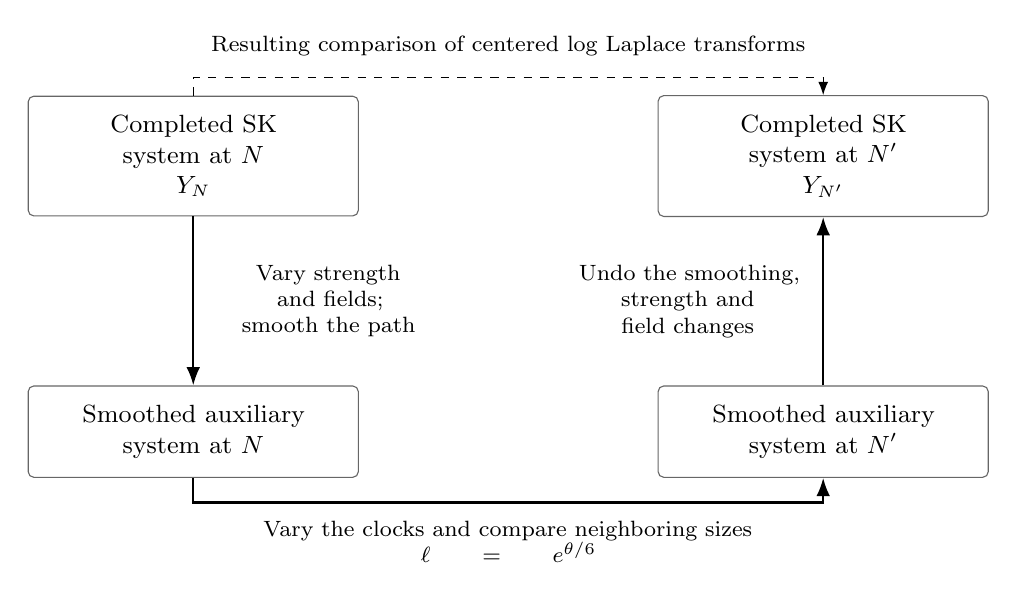
\begin{tikzpicture}[>=Latex,node distance=14mm,
 box/.style={draw=black!60,rounded corners=2pt,align=center,inner sep=7pt,text width=37mm,font=\small},
 lab/.style={font=\footnotesize,align=center,fill=white,inner sep=3pt}]
\node[box] (a) at (0,3.5) {Completed SK system at $N$\\$Y_N$};
\node[box] (b) at (8,3.5) {Completed SK system at $N'$\\$Y_{N'}$};
\node[box] (c) at (0,0) {Smoothed auxiliary\\system at $N$};
\node[box] (d) at (8,0) {Smoothed auxiliary\\system at $N'$};
\draw[->,thick] (a)--(c) node[midway,right,lab,text width=32mm] {Vary strength\\and fields;\\smooth the path};
\draw[->,thick] (c.south)--(0,-.9)--(8,-.9)--(d.south);
\node[lab,text width=105mm] at (4,-1.4) {Vary the clocks and compare neighboring sizes\\$\ell=e^{\theta/6}$};
\draw[->,thick] (d)--(b) node[midway,left,lab,text width=32mm] {Undo the smoothing,\\strength and field changes};
\draw[->,dashed] (a.north)--(0,4.5)--(8,4.5)--(b.north);
\node[lab,text width=105mm] at (4,4.9) {Resulting comparison of centered log Laplace transforms};
\end{tikzpicture}
\caption{The route from $N$ to an arbitrary $N'\in[N,2N]$. The displayed endpoints are the centered, rescaled bare systems. The proof bounds the changes along the route and the errors from the small regularizations at its ends. One parameter vector is selected for each finite route and each Laplace test.}
\label{fig:comparison-path}
\end{figure}


The comparison rests on four estimates.
\begin{enumerate}
\item We solve the linear equations for covariances of overlap errors.
The inverse bound remains uniform when the hierarchy is refined or its
masses become small. Summation by parts cancels the small-mass
denominators. Contributions from branching at an already specified
vertex are retained in the bound.
\item We vary the matrix and field covariances to turn pressure
comparisons into bounds on mean squared overlap errors. The constrained
minimization requires estimates in both the mass coordinate and the
quantile's value. A derivative of the minimum controls every minimizer,
so the argument does not need to select a minimizer measurably.
\item We obtain higher moments for the actual comparison paths by
projecting spin observations onto their revealed Gaussian histories and
integrating squared martingale increments. Before integrating a centered
quantity over a moving branch point, we show that the paths retained in
the calculation have a law independent of that point.
\item We sum the signed pressure coefficients before taking absolute
values. Summing the scalar contributions above a fixed cut, combining
the quadratic correction, and rescaling size cancel the leading terms
of degrees two, three, and four. The remaining increments are summable.
\end{enumerate}

\subsection{Consequences}

Theorem~\ref{thm:main} and the variance asymptotic above instantiate
the ferromagnetic comparison of Dey and Kang
\cite[Proposition~1.5]{DeyKang2026}. The comparison does not establish
the zero-field law, but it gives the following consequence once that
law and its positive variance prefactor are available.

\begin{corollary}[SK--Curie--Weiss fluctuations below unit coupling]
\label{cor:skcw}
Fix $\beta>1$ and $0\le\gamma<1$. Using the same independent standard
Gaussian couplings as in \eqref{eq:model}, define the exponent and log
partition function
\[
 \begin{gathered}
 \mathcal H_n^{\mathrm{CW}}(\sigma;\beta,\gamma)
 =
 \frac{\beta}{\sqrt n}\sum_{1\le i<j\le n}g_{ij}\sigma_i\sigma_j
 +\frac{\gamma}{2n}\left(\sum_{i=1}^n\sigma_i\right)^2,\\
 F_n^{\mathrm{CW}}(\beta,\gamma)
 =\log\sum_{\sigma\in\{-1,1\}^n}
 e^{\mathcal H_n^{\mathrm{CW}}(\sigma;\beta,\gamma)}.
 \end{gathered}
\]
Here $\gamma$ is the ferromagnetic coupling already in the exponent.
As $n\to\infty$ through all integers,
\[
 \begin{gathered}
 \Var F_n^{\mathrm{CW}}(\beta,\gamma)
 \sim a_2(\beta)n^{1/3},\\
 \frac{F_n^{\mathrm{CW}}(\beta,\gamma)
       -\mathbb E F_n^{\mathrm{CW}}(\beta,\gamma)}
      {\sqrt{\Var F_n^{\mathrm{CW}}(\beta,\gamma)}}
 \Longrightarrow\nu_\beta.
 \end{gathered}
\]
Here $a_2(\beta)>0$ is the constant $a_2$ above at the same $\beta$.
The centering and standard deviation are the perturbed model's own
exact finite-size quantities.
\end{corollary}

The comparison controls the added free energy in $L^2$ uniformly in
$n$. Since the unperturbed standard deviation grows like $n^{1/6}$,
this error disappears after either model's exact standardization.
The full argument is in Section~\ref{sec:consequences}.

This consequence is confined to the displayed zero-field ordered
Gaussian model at fixed $\beta>1$ and $0\le\gamma<1$; it does not cover
$\gamma=1$ or a coupling varying with $n$.

For the original zero-field model, the variance asymptotic also gives
the following consequence of Chatterjee's general Gaussian and
replacement inequalities.

\begin{corollary}[Upper disorder-chaos scales in zero-field SK]
\label{cor:disorder-chaos}
Fix $\beta>1$ and $n\ge2$. Put $E_n=\{(i,j):1\le i<j\le n\}$ and
$M=|E_n|=n(n-1)/2$, and let $g'$ be an independent copy of
$g=(g_{ij})_{(i,j)\in E_n}$ in \eqref{eq:model}. Write
$\langle\cdot\rangle_{g,h}$ for expectation under the product of that
model's Gibbs laws with disorders $g,h$, and
$R=n^{-1}\sum_i\sigma_i\tau_i$ for the overlap. Thus the replicas are
independent conditional on their disorders; $\mathbb E$ below also
averages the disorder and any replacement set.

For $t>0$, set $g^t=e^{-t}g+\sqrt{1-e^{-2t}}\,g'$. For an integer
$0\le k\le M$, let $A$ be independent of $g,g'$ and uniform over the
$k$-element subsets of $E_n$. Set $g^A_{ij}=g'_{ij}$ on $A$ and
$g^A_{ij}=g_{ij}$ otherwise. Then
\begin{align}
 \mathbb E\langle R^2\rangle_{g,g^t}
 &\le \frac1n+\frac{2\Var F_n(\beta)}
                 {\beta^2n(1-e^{-t})},\label{eq:chaos-ou}\\
 \mathbb E\langle R^2\rangle_{g,g^A}
 &\le \frac1n+\frac{2(M+1)\Var F_n(\beta)}
                 {\beta^2n(k+1)}+C_\beta n^{-1/2},\label{eq:chaos-replacement}
\end{align}
for a finite constant $C_\beta$ depending only on $\beta$. As $n\to\infty$, for
$t_n\ge0$ and integers $0\le k_n\le M$, these bounds imply
\[
 \begin{aligned}
 t_n n^{2/3}\to\infty
 &\quad\Longrightarrow\quad
 \mathbb E\langle R^2\rangle_{g,g^{t_n}}\to0,\\
 (k_n/M)n^{2/3}\to\infty
 &\quad\Longrightarrow\quad
 \mathbb E\langle R^2\rangle_{g,g^{A_n}}\to0,
 \end{aligned}
\]
where $A_n$ has size $k_n$ as above.
\end{corollary}

Chatterjee's variance identity and replacement inequality bound the
mean squared overlap by the free-energy variance. Substitution of the
$n^{1/3}$ variance asymptotic gives the displayed sufficient scales;
Section~\ref{sec:consequences} checks both normalizations.

These are sufficient annealed perturbation scales, not a sharp
transition or a quenched statement. No overlap conclusion is asserted
for the SK--Curie--Weiss model in Corollary~\ref{cor:skcw}.

\subsection{Organization and order of limits}

Sections~\ref{sec:foundations}--\ref{sec:paths} develop the finite-tree
calculus and admissible comparison paths. The pair inverse in
Section~\ref{sec:inverse} first supplies the global trial accuracy of
Section~\ref{sec:global}; that accuracy and the local auxiliary comparisons
give the genuine-path budgets of Section~\ref{sec:budgets}. The analytic
inputs for the modified optimizers are proved within that section before
their use. Section~\ref{sec:statistics} derives genuine-path statistics
from the budgets and uses the pair inverse again in its high-mass
covariance equation. Scalar compression in Section~\ref{sec:expansion}
and the common parameter order in Section~\ref{sec:parameters} complete
Proposition~\ref{prop:increment}. The conditional deduction in
Section~\ref{sec:reduction} then gives full-sequence moment convergence,
positive limiting variance, moment determinacy, the finite-system law
specification, and exact finite-size standardization. Section~\ref{sec:consequences}
contains the proofs of the two corollaries stated above.

All conclusions are for a fixed $\beta>1$. Moment orders, expansion orders, and propagation depths are finite and fixed before $N\to\infty$. Their values may depend on the desired estimate. The exponent used for the small Laplace test is chosen only after the power saving in the increment estimate is established.

\section{Hierarchical Gaussian calculus}
\label{sec:foundations}

The size comparison uses two kinds of calculation: expectations under
hierarchical probability laws, and signed sums of such expectations produced
by covariance differentiation. We define these separately. The resulting
finite-order cavity and size expansions express pressure changes in terms
of overlap errors relative to a one-site scalar model.

\subsection{Normalization and positive tree laws}

We refer to \cite{PE} as PE; references explicitly marked PE concern that
paper. Fix \(T=\beta^2>1\). As in \eqref{eq:completed-free-energy}, we
add an independent spin-constant Gaussian of variance \(T/2\) and use the
uniform probability prior on spins. The resulting matrix covariance is
\(mTQ^2/2\), where \(Q\) is the overlap defined below. The added Gaussian
has bounded moments, and replacing the counting prior by the probability
prior shifts only the mean.

We work in dyads \(N\le m\lesssim 2N\) (with small enlargements), \(m\) the integer number of sites, and put \(x=N^{-1/6}\). All exponents below, including any order of a Taylor expansion, are fixed as \(N\to\infty\); constants can depend on these choices and on \(T\). We use ``with subpower loss'' or \(\lesssim_\circ\) to allow \(C_\epsilon x^{-\epsilon}\) for \emph{every} sufficiently small fixed \(\epsilon>0\). ``Power small'' means \(O(x^c)\) for some fixed \(c>0\); for assertions in every fixed \(L^p\) a power saving not indexed by \(p\) means the exponent is independent of the fixed finite moment order (constant and threshold need not be). Power slack choices in estimates with an indicated hierarchy of exponents are made before using subpower losses.

Estimates in this dyadic notation apply with \(N/2\le m\le3N\); changing comparison scales by bounded factors from this convention is immaterial. Several pieces have local variables (including error majorants and truncation orders) redefined in each calculation. In particular the path martingale \(X_v\) below is unrelated to the notation for the standardized free energy, and in Section~\ref{sec:budgets} the letter \(X\) without a path subscript is also used for a scale ratio.

Fix a terminal mass \(a\in[1,4]\). The coordinate \(v\in(0,a)\)
is the replica mass, and the deterministic nonnegative nondecreasing
functions \(b,h\) are the matrix and spin-field clocks. Jumps are allowed.
Their cumulative Gaussian covariance at mass \(v\) is
\[
 m(b(v)Q^2/2+h(v)Q),\qquad
 Q=m^{-1}\sum_{i\le m}\sigma_i\sigma'_i.
\]
For step clocks, construct independent Gaussian increments with these
covariance increases, including any initial increment at mass zero.
If \(H\) is their sum, the terminal continuation is
\(a^{-1}\log\int e^{aH}\), with the integral taken against the uniform
probability prior. Compute earlier continuations backwards: for an
increment at mass \(v>0\), set
\[
 F_{\rm before}=v^{-1}\log\mathbf E\exp(vF_{\rm after}),
\]
where this expectation averages only that increment. At mass zero use
ordinary expectation. Divide the resulting deterministic value by \(m\)
and subtract \(a(b(a-)/4+h(a-)/2)\); this defines the self-corrected
pressure \(f_m(b,h)\). Its interval length \(a\) will be implicit.

The same continuations define a forward probability law. Reveal each
Gaussian increment with its original Gaussian density multiplied by
\(\exp(v(F_{\rm after}-F_{\rm before}))\), and then draw the terminal
spin from the Gibbs law of exponent \(a\). The backward recursion makes
each transition integrate to one. On a fixed finite rooted tree, branches
share the increments before their fork and use conditionally independent
forward transitions afterwards. We call this the \emph{positive tree law}
and write \(\nu[P]\) for its expectation of \(P\), including both fields
and terminal spins. The tree topology and clocks are fixed in this
expectation. Bounded monotone clocks are obtained by the fixed-site step
limits from PE stated below.

A specified observation may lie on either side of a jump or at an
intermediate clock value. At a simultaneous jump we use the joint filling
\[
 (b_t,h_t)=(b_-,h_-)+t(\Delta b,\Delta h),\qquad 0\le t\le1,
\]
with mass held fixed, and preserve this filling in step approximations.
Endpoint tree laws and mass-integrated identities do not depend on the
order of revelation within a same-mass jump. The separate matrix and
field contributions to quadratic variation, and observations at
intermediate cuts, do use the prescribed filling.

For a single path let \(y=\sigma/\sqrt m\),
\[
\begin{gathered}
 X_v=\mathbf E_v y,\qquad C_v=\mathbf E_v(y-X_v)(y-X_v)^{\mathsf T},\\
 S_v=\mathbf E|X_v|^2,\qquad
 B_v=\mathbf E\|\mathbf E_v yy^{\mathsf T}\|_{\rm HS}^2,\qquad D_v^2=B_v-S_v^2.
\end{gathered}
\]
Here \(\mathbf E_v\) is conditional expectation given the fields revealed
through the specified cut, and \(\mathbf E\) averages the full single-path
positive law. Thus \(X_v,C_v\) are functions of the random prefix, whereas
\(S_v,B_v,D_v\) are deterministic statistics of that law. Write \(H_v\)
for the Hessian of the continuation with respect to a source coupled to
\(y\) in the downstream Hamiltonian, with the revealed prefix held fixed. Put
\(L_v=y\cdot X_v-|X_v|^2/2\) and
\(W_v=(y-X_v)^{\mathsf T}H_v(y-X_v)\). These last two observables also
retain the terminal spin.

\subsection{Pinned moments and projection}

The next estimates distinguish a variation of the deterministic clocks
from movement along one fixed revealed path. In the pressure formula,
\(db(v),dh(v)\) are clock variations in an external parameter. In
the susceptibility inequality, \(dS_v\) and \(dh\) are instead
Stieltjes increments along the fixed path, including its prescribed
filling at a jump. The source Hessian \(H_v\) always keeps the
revealed prefix fixed.

\begin{lemma}[Pressure, source, and single-path estimates]
\label{found:estimates}
For the positive laws just defined, the following identities and
inequalities hold at every fixed size. The moment bounds in
\eqref{eq:A1}--\eqref{eq:A2} hold for every fixed real \(2\le p<\infty\),
with deterministic \(k\in L^2(0,a)\) and zero deterministic external
field.
\[
\begin{split}
 df_m&=-\tfrac14\int B_v\,db(v)\,dv-\tfrac12\int S_v\,dh(v)\,dv,\\
 vC_v\preceq H_v\preceq a C_v,\qquad
 d S_v&\ge m\,\mathbf E\operatorname{tr}H_v^2\,dh,\qquad
 \mathbf EW_v=\mathbf E\operatorname{tr}C_v H_v,\\
 \left\|\int k_v(L_v-\mathbf EL_v)dv\right\|_p^2&\le c_p\left\|\int k_v^2 W_v\,dv\right\|_{p/2}.
\end{split}                                                    \tag{A1}\label{eq:A1}
\]
The last line is a moment estimate under the full single-path law, with
deterministic weights \(k_v\) and zero deterministic external field.
More generally, for
polynomials \(P_v\) of fixed degree with bounded deterministic coefficients,
\[
 \left\|\int k_v(P_v(L_v)-\mathbf E P_v(L_v))dv\right\|_p^2
 \le c_p\left\|\int k_v^2 P'_v(L_v)^2 W_v\,dv\right\|_{p/2}.
                                                               \tag{A2}\label{eq:A2}
\]

For the projection bound only, assume that the total clocks are at most
a fixed power of \(\log N\), and that the positive mass and field
length are bounded below by inverse powers of \(N\). If a branch
has traversed a pure or mixed clock interval with field length
\(\Delta h>0\) after separating from the data determining an anchor
vector \(V\), and its mass is at least \(v>0\) throughout that
interval, then for every fixed even \(p\ge2\),
\[
 \|V\cdot(y-X_{\rm end})\|_p
 \lesssim_p \frac{\log^2 N}{v\sqrt{m\Delta h}}\,\|V\|_p                       \tag{A3}\label{eq:A3}
\]

where the vector norm inside \(L^p\) is Euclidean. The branch must
retain its normalized future kernel conditional on the prefix and outside
data; in particular, the bound applies to conditionally independent
resamplings.
\end{lemma}

\begin{proof}
Equations \eqref{eq:A1} and \eqref{eq:A3} are the pressure, source,
pinned-moment, and projection estimates of \cite[Lemmas~2.1--2.3
and~3.5, equations~(1) and~(13)]{PE}. To match the terminal-mass-one
normalization there, put
\[
 u=v/a,\qquad \widetilde b(u)=a^2b(au),\qquad
 \widetilde h(u)=a^2h(au),\qquad \widetilde F=aF.
\]
The conditional spin means and covariances are unchanged, while
\(H_{au}=a\widetilde H_u\). The projection denominator is unchanged
as well, since \((v/a)\sqrt{m a^2\Delta h}=v\sqrt{m\Delta h}\).
Appendix~\ref{sec:companion-interface} records the pressure and moment
conversions. The fixed-size path-limit result is PE, Proposition~2.14.

For \eqref{eq:A2}, we include the polynomial argument of PE,
Appendix, paragraph ``Source and pressure calculus; the scope of pinned
moments.'' Pin the terminal spin and write the Gaussian increments in
terms of standard Gaussian drivers, as in the proof of PE, Lemma~2.3. Let \(\mathsf A_v\) be the Hessian of the continuation
in these drivers and \(\mathsf B_v\) its mixed Hessian with the
normalized spin source. After the transition densities telescope, the
negative logarithm of the pinned driver density is the Gaussian
quadratic potential minus \(aH_\sigma\), which is linear, plus
\(\int_0^a F_v\,dv\), where \(F_v\) is the continuation at the cut
\(v\). Consequently
\[
 \begin{pmatrix}\mathsf A_v&\mathsf B_v\\
 \mathsf B_v^{\mathsf T}&H_v\end{pmatrix}\succeq0,
 \qquad
 \mathsf Q=I+\int_0^a\mathsf A_v\,dv,
\]
where \(\mathsf Q\) is the Hessian of the negative logarithm of the
pinned driver density. The driver gradient of \(L_v\) is
\(g_v=\mathsf B_v(y-X_v)\). Thus, for every driver direction \(z\),
\( |z\cdot g_v|^2\le(z^{\mathsf T}\mathsf A_vz)W_v\).
For the polynomial observable set
\[
 G_P=\int_0^a k_vP'_v(L_v)g_v\,dv,
 \qquad R_P=\int_0^a k_v^2P'_v(L_v)^2W_v\,dv.
\]
Cauchy--Schwarz in \(v\) gives
\( |z\cdot G_P|^2\le(z^{\mathsf T}\mathsf Qz)R_P\), hence
\(G_P^{\mathsf T}\mathsf Q^{-1}G_P\le R_P\).
The inverse-Hessian Brascamp--Lieb inequality~\cite[Theorem~4.1]{BL1976}
therefore gives \eqref{eq:A2} for \(p=2\). Applying the same variance
inequality to the \(p/2\)-th absolute power of the centered integral,
as in PE, Lemma~2.3, gives the assertion for every fixed \(p>2\).

The zero-field spin gauge transformations act transitively on terminal
spins and preserve both \(L_v\) and \(W_v\). Because the coefficients of \(P_v\) and the weights \(k_v\)
are deterministic, they also preserve the polynomial integral and
\(R_P\). Their conditional laws are consequently independent of the
pinned spin, including the mean used for centering. Averaging over that
spin yields the full single-path estimate. Bounded-weight approximation
and then the fixed-\(m\) path limit give the stated range of clocks
and weights.

Clocks are bounded for each \(N\), possibly by a power of \(\log N\); \eqref{eq:A1} is clock independent. For \eqref{eq:A3}, we apply PE, equation~(13), only in this bounded or polylogarithmic clock regime; together with the polynomial mass and field-length bounds, this gives the polynomial coefficient-ratio bounds needed in its moment iteration, as detailed in Appendix~\ref{sec:companion-interface}. Our estimates can always be passed from affine finite-step interpolations, or from inserted fixed cuts, by the fixed-\(m\) limit assertion, keeping chosen revelation sides and the joint filling at observed intermediate jump cuts, and using the corresponding integrated inequalities. In particular no discretization \emph{rate} in \(m\) is used.

The pinned inequalities in this lemma concern the full single-path law. When a tree contains additional branches, we first marginalize the branches not used by the test. Random factors retained on other branches are subsequently handled by unconditional H\"older inequalities; they are not made into random weights in \eqref{eq:A2}.
\end{proof}

\subsection{Signed allocation of replica labels}

Covariance derivatives introduce additional replica labels. For a simple
example, start with one observed leaf above a cut \(v\), and divide its
edge at a level \(u\in(v,a)\). An extra label may coincide with that
leaf, with coefficient \(a\), or split from it along either edge
interval, with coefficient minus the interval length. On a constant
summand the total is \(a-(a-u)-(u-v)=v\). In a larger tree, attachment
to a fork also contributes an atom. We sum all these placements by the
signed rule of PE, Section~2,
Proposition~2.5, equation~(2), and Lemmas~2.6, 2.8, and~2.9. A new
label coinciding with an observed leaf has coefficient \(a\); a new
split on an occupied edge has coefficient \(-dv\); attachment at an
existing mass-\(v\) fork with \(d\) children has coefficient
\(-(d-1)v\). These coefficients multiply expectations under the
positive laws just defined. They are not probabilities.

The row-sum rule sums one free label whose summand is constant over all
its attachments in a block above a cut \(v\). The result is that constant
times \(v\), as in the example. A row whose summand depends
on its attachment cannot be collapsed this way. Empty levels can be
inserted continuously without changing the calculation. Different
infinitesimal fork variables specify different tree vertices even when
the covariance clocks have the same value at those vertices.

A sum \emph{per root mass}, denoted by \((\cdot)_\#\), begins without
specified old labels. Its first label is an ordinary observation with
weight 1, and all subsequent labels use the signed rule. This is the
limit of normalized summation as the incoming mass tends to zero. Sums
without \(\#\) extend whatever old labels are already present.
Products of symbolic slot polynomials concatenate all their labels;
a coefficient involving only some labels is evaluated on the restriction
of the final topology to those labels. The labeled product rules in PE,
Proposition~2.5 make this convention associative, commutative, and
independent of allocation order. In a per-root product we concatenate first and apply the root
normalization only once.

Constant diagonal covariance changes contribute only to the self
correction. Thus pressure insertions after that correction use ordered
off-diagonal pairs and a factor \(1/2\) per insertion. The first
insertion gives \eqref{eq:A1}; for subsequent insertions the constant
diagonal terms cancel by the row-sum rule in PE, equation~(2). The same
rule applies to any affine positive semidefinite interpolation between
finite feature models with constant diagonal and fixed \(a\), after
subtracting \(a/2\) times the terminal diagonal. For total pressures,
the inserted covariance change is the total covariance change, rather
than its per-site value. Deterministic additive terms common to the two
ensembles cancel when we take their pressure difference.

Enlarging a positive-law tree preserves its original marginals. For any
fixed number of inserted labels, the total variation of the signed
allocation coefficients is uniformly bounded. Taking absolute values
in placement order leaves finitely many integrals over new fork masses,
existing-fork atoms with bounded multiplicities times their masses,
and terminal coincidences. We may therefore reorder the exact signed
sum with its topology restrictions first, and then estimate with this
absolute allocation measure. This order of operations is essential
when a later argument uses cancellation.

\subsection{Scalar references and Laplace tests}

The signed calculus will compare the matrix model with independent
one-site scalar systems. For the reference model take one spin and only a deterministic spin clock
\(K(v)\). Its continuation can be parametrized by cumulative variance
\(t\) instead of mass. The mass already reached by time \(t\) is
\(\alpha(t)=|\{v\in(0,a):K(v)\le t\}|\). Write \(V(t,z)\) for
the scalar continuation at field \(z\), and \(Z_t\) for its field under
the forward positive law. They satisfy
\[
 V_t=-\tfrac12(V_{zz}+\alpha V_z^2),\qquad dZ_t=\alpha V_z(t,Z_t)dt+dB_t ,
 \qquad V_{\rm term}=a^{-1}\log\cosh(a z).
\]
Set \(\Gamma(t)=\mathbf E V_z(t,Z_t)^2\), with zero starting field
unless otherwise stated. A terminal mass-\(a\) extension in scalar time
changes earlier continuation values only by a spatial constant. In
particular it leaves their derivatives in \(z\) unchanged. On a fixed
tree let \(\tau_i\) be the scalar spin at leaf \(i\), and let
\(v_{ij}\) be the mass where distinct leaves \(i,j\) separate.
Their positive-law moment is
\(\nu_K[\tau_i\tau_j]=\Gamma(K(v_{ij}))\). Common covariance insertions and source derivatives of these moments again use the tree calculus. In particular any fixed spatial derivative of positive order of \(V\) is bounded uniformly (even with long but finite clocks). Below put
\[
 q(v)=\Gamma(K(v)),\qquad h_*(v)=K(v)-b(v)q(v),\qquad d(v)=h(v)-h_*(v).
\]

The physical paths used below have \(b(v)=b(0+)\) and \(h(v)=0\)
for \(v<x\). For \(0<s<x\), move the initial matrix revelation
from mass zero to mass \(s\). This gives the tilted pressure
\(f_m^s=f_m(b\,{\bf1}_{v\ge s},h)\); the untilted pressure is
\(f_m^0=f_m(b,h)\). Put \(\psi_m(s)=f_m^s-f_m^0\). The factor
\({\bf1}_{v_{ij}\ge s}\) records whether two tilted branches share
the matrix revelation. Accordingly define \(Q^*_{ij}=Q_{ij}\) in
the untilted ensemble and
\(Q^*_{ij}={\bf1}_{v_{ij}\ge s}Q_{ij}\) in the tilted ensemble.
The mass-\(s\) power mean then gives
\[
 {\cal K}_m(s)=s\,m\psi_m(s)=\log\mathbf E\exp\{s(G_m-\mathbf E G_m)\},
                                                               \tag{A4}\label{eq:A4}
\]
where \(G_m\) is the random total continuation just after the initial matrix revelation in the untilted path. Each connected subtree with internal splits at \(v\ge s\) in a tilted positive law has its untilted marginal reweighted by \(\exp(sG_m)/\mathbf E\exp(sG_m)\). Distinct such components have independent roots. Products using active branches from more than one component can therefore be bounded by their active-subtree marginal norms without interpreting the forest as sharing an untilted root. Set
\[
 \Delta=Q^*-q,\qquad J=h+b Q^*-K=b\Delta+d
\]
on off-diagonal pairs. Scalar paths used as references are \emph{unshifted} in both ensembles. Tests involving matrix-model overlaps only through \(Q^*\) are invariant under simultaneous sign flip of all spins on a component (with its high ordinary fields negated); consequently at every pair \(ij\), including below \(s\) in the tilted case, \(\nu[P Q_{ij}]=\nu[P Q^*_{ij}]\) for these spin tests.

\subsection{Finite row and size expansions}

We now encode fixed finite Taylor expansions in the row mismatch \(J\).
A \emph{jet} means that the series is retained only through a specified
finite degree; no convergence of an infinite series is being asserted.
In all inserted pairs, the two ends must be different leaves, although
labels from different pairs may coincide. Define the symbolic series
\[
 \Psi_K(J)=\left\langle\exp\{\tfrac12\sum J_{cd}\tau_c\tau_d\}\right\rangle_K,
 \qquad N_{ij,K}(J)=\left\langle\tau_i\tau_j
                \exp\{\tfrac12\sum J_{cd}\tau_c\tau_d\}\right\rangle_K .         \tag{A5}\label{eq:A5}
\]
To read \eqref{eq:A5}, first expand the exponential to the required
finite degree and allocate its pair labels. For each final topology,
the brackets are the positive scalar moment of the labels in that
coefficient. Multiply coefficients on their respective restricted
topologies before carrying out the signed allocation sum. Thus
\(\log\Psi\) has the ordinary joint scalar cumulants at each fixed
topology as its coefficients. Products, differentiation, and inversion
of the series with constant term 1 are all finite-degree polynomial
operations under this convention.

For example, in the product of two
scalar coefficients \(\nu_K[\tau_i\tau_j]\nu_K[\tau_c\tau_d]\), allocate
all four labels on one final topology, then evaluate the first moment
on its \(ij\) restriction and the second on its \(cd\) restriction.
Their product is not the four-spin moment, even when some labels
coincide. The clock derivative and the coefficient linear in the number
of added sites will be expressed through the same pressure symbol,
namely
\[
 {\cal I}=\log\Psi_K(J)-\tfrac14\sum b_{ij}(Q^*_{ij})^2 .
                                                               \tag{A6}\label{eq:A6}
\]
Independent additive deterministic per-root terms in this symbol will always cancel.

The following Taylor rules require a monotone reference \(K\) and
bounded \(h-K\) and \(b\). A remainder with \(k\) insertions is a
finite sum over boundedly many allocated labels, possibly integrated
over interpolation parameters. Its integrand is a bounded factor times
\(k\) specified overlap insertions on off-diagonal pairs. We estimate
such terms using the absolute allocation measure and a positive
probability law.

The intermediate law may still contain one interpolated scalar row.
For a nonnegative spin test of the other rows, PE, Lemma~2.9 compares
this law to the actual law up to a constant: its Gr\"onwall bound uses
the bounded total covariance change of that row. Deleted sites are
omitted from an overlap without changing its denominator \(m\).
Restoring those sites changes a bounded Lipschitz polynomial of fixed
degree by \(O(m^{-1})\). Any deterministic topology coefficient or
weight multiplying the test also multiplies this error bound. Throughout
this interpolation the spin test is fixed, so it contributes no
additional derivative.

\begin{lemma}[Finite cavity quotient]
\label{found:cavity-quotient}
For overlap-polynomial \(P\) invariant as after \eqref{eq:A4}, on any fixed finite-label tree including \(ij\), one has through order \(k-1\)
\[
 \nu[P Q^*_{ij}]=\nu[P(N_{ij,K}/\Psi_K)_{<k}]
          +{\rm Rem}_k+O(m^{-1}),                                      \tag{A7}\label{eq:A7}
\]
where \({\rm Rem}_k\) has at least \(k\) insertions \(J\), times \(P\).
\end{lemma}

\begin{proof}
By exchangeability, the observed overlap may be represented using one
chosen site. Delete that site's contribution from the other tested
overlaps, retaining the denominator \(m\), and interpolate its Gaussian
kernels to those of an independent one-site scalar model with clock
\(K\). All other covariance kernels remain fixed. Both endpoints are
positive semidefinite, as is their affine interpolation. In the expansion
back from the independent endpoint, the covariance insertion is
\(J_{cd}\tau_c\tau_d\), where \(J\) uses the remaining-row overlap
and the mask of the actual matrix clock. The omitted terms are
\(O(m^{-1})\) and constant diagonals. The row covariance change is
bounded, so Taylor's integral remainder has the form described above.

At the independent endpoint, averaging the removed spin gives
\(\Psi_K\) when it is unobserved, and \(N_{ij,K}\) when its product
on leaves \(i,j\) is observed. Expanding the former against the
truncated quotient \(N_{ij,K}/\Psi_K\) cancels its factor \(\Psi_K\)
to the retained order. Allocation order symmetry identifies the terms
on each final topology and gives \eqref{eq:A7}. Products here multiply
separately averaged scalar coefficients; they do not couple their
scalar spins. In particular the linear cavity kernel on a pair \(cd\) is
\[
 {\bf M}_{ij,cd}=\tfrac12
 (\nu_K[\tau_i\tau_j\tau_c\tau_d]-\nu_K[\tau_i\tau_j]\nu_K[\tau_c\tau_d]).
                                                                    \tag{A8}\label{eq:A8}
\]
This proof also gives the unestimated remainder representation using one interacting scalar row (the removed site) along the affine interpolation, if symmetries must be used before taking absolute values.

\end{proof}

\begin{lemma}[Change of scalar reference]
\label{found:reference-change}
Apply \eqref{eq:A7} at a monotone reference \(K'\), then Taylor-expand
its deterministic scalar coefficients from \(K\) to \(K'\). At any
consistent total truncation, the result is the quotient with reference
\(K\) and combined argument
\(J=(h+bQ^*-K')+(K'-K)\).
\end{lemma}

\begin{proof}
PE covariance differentiation, equation~(2), represents a derivative
of a scalar coefficient by a new pair insertion
\((K'-K)_{cd}\tau_c\tau_d/2\). Allocation order symmetry permits us
to combine these with the insertions already present in the quotient.
The apparent extra factors \(\Psi_K(K'-K)\) have no effect on an
observed topology whose spin test is independent of the new labels:
after allocating these labels last, every positive-degree term is a
derivative of the unit scalar moment and sums to zero. For a standalone
per-root sum the same terms can remain, but they are deterministic.
Taylor's integral remainder has bounded scalar coefficients and powers
of \(K'-K\); it can also retain ordinary polynomial factors of the
original argument \(h+bQ^*-K'\).
\end{proof}

\begin{lemma}[Differentiated row identity]
\label{found:row-derivative}
Let a dot vary \(b,h,K,q\) at fixed interval length \(a\), and let
\({\cal D}\) differentiate \eqref{eq:A6} including its scalar coefficients,
with the formal rule \({\cal D}\Delta=-e\Delta\) for any fixed \(e\).
Thus \({\cal D}Q^*=\dot q-e\Delta\); this rule acts on the symbolic
polynomial and does not differentiate a random spin sample. Up to
deterministic terms common to the two ensembles and Taylor remainders,
\[
 \dot f_m^{\,s}\ \equiv\ (\nu[{\cal D}{\cal I}])_\#.                   \tag{A9}\label{eq:A9}
\]
The same formula applies with superscript \(s=0\). The error and its differentiated weights are as described in the proof below.
\end{lemma}

\begin{proof}
Differentiating a scalar coefficient inserts
\(\dot K_{ij}\tau_i\tau_j/2\). This cancels the \(-\dot K\)
part of \({\cal D}J\); terms with no previously attached labels
are deterministic. Thus the logarithm contributes
\[
 \frac12\sum\frac{N_{ij,K}}{\Psi_K}
       (\dot h+\dot b Q^*+b{\cal D}Q^*)_{ij}.
\]
Apply \eqref{eq:A7} to replace the quotient by \(Q^*\), with its
stated error. The term \(bQ^*{\cal D}Q^*/2\) then cancels the
corresponding derivative of the quadratic term in \eqref{eq:A6}.
In particular the choice of \(e\) disappears. The terms left are
\(\frac12\sum\dot h Q^*+\frac14\sum\dot b(Q^*)^2\), precisely
the off-diagonal pressure insertions in \eqref{eq:A1}.

For the error, all tests have bounded degree and at most one
differentiated weight. If \(\log\Psi\) is truncated after degree
\(k\), the residuals in the difference of the two pressure derivatives
have at least \(k\) insertion factors. They also have one weight at
a split, possibly on an additional pair, bounded by a constant times
\[
 1+|\dot h|+|\dot b|+|\dot K|+|\dot q|;
\]
the 1 is omitted when \(e=0\). The \(O(m^{-1})\) errors carry the
same weights. This follows from the product rule, since differentiating
one insertion can remove that factor, and from \eqref{eq:A7}. If a
second reference \(K'\) is used, expand the quotient in this gradient
first, then recombine by Lemma~\ref{found:reference-change}. This does
not require differentiating \(K'\).

There is one truncation convention to check. Differentiating an
insertion lowers its insertion degree by one, whereas differentiating
a scalar coefficient does not. Through degree \(k\) in the old
\(J\) factors, the coefficient part of \({\cal D}\Psi\) therefore
inserts \(\frac12\sum(N_{ij,K})_{\le k}\dot K_{ij}\), formally
including its degree-zero term. In a product with old labels independent
of the new placements, that term sums to zero when the new labels are
allocated last: it differentiates a unit scalar observation. Standalone
per root, its discrepancy is common and deterministic. Thus coefficient
differentiation of the logarithm uses the reciprocal jet through degree
\(k\), while differentiation of an insertion uses the quotient through
degree \(k-1\). All these cancellations take place in the unrestricted
signed sums, before imposing split-scale restrictions for estimates.

\end{proof}

\begin{lemma}[Finite increments in the number of sites]
\label{found:size-increment}
At fixed clocks and \(s\), assume that \(bq^2\) is nondecreasing. For every fixed positive integer \(j\), the change from \(m\psi_m\) to \((m+j)\psi_{m+j}\), expanded through total order \(k\), is a polynomial in \(j\) of degree at most \(k\) with zero constant term. Its linear coefficient is the difference of the per-root expectations of \eqref{eq:A6}, with \(\log\Psi\) truncated after degree \(k\). The remainder has the total-pressure bounds given below.
\end{lemma}

\begin{proof}
For size changes at fixed clocks and \(s\), compare \((m+j)\psi_{m+j}\) to \(m\psi_m\), with any fixed positive integer \(j\). Interpolate the enlarged kernel from that of \(m\) old spins plus \(j\) independent scalar rows at \(K\), to its actual value plus independent, spin-constant cumulative covariance \(j b q^2/2\) (assume \(b q^2\) nondecreasing). This addition gives the same pressure shift for both tests. The off-diagonal insertion before the factor \(1/2\) is
\[
 J\sum_{h'=1}^j\tau^{h'}\tau^{h'\prime}
       -\tfrac j2 b(Q^{*2}-q^2)+O_j(m^{-1}).
\]
Indeed the normalization of the matrix feature changes from \(m\) to \(m+j\) while field terms are additive. This difference is bounded. Taylor through order \(k\) in the total pressure now gives a polynomial in \(j\) of degree \(\le k\), constant term zero; its coefficient linear in \(j\) is the compared per-root expectation of \eqref{eq:A6}, \(\log\Psi\) truncated after degree \(k\). For the linear coefficient, group the labeled insertions by their
assigned scalar row. The scalar rows are independent on each fixed
topology, so their series is \(\Psi_K^j\). If \(C\) denotes the
matrix counterterm \(\frac14\sum b(Q^{*2}-q^2)\), the combined series
is \(\Psi_K^j e^{-jC}\). Its coefficient of \(j\) is
\[
 [j]\big(\Psi_K^j e^{-jC}\big)=\log\Psi_K-C.
\]
The deterministic \(q^2\) term cancels between the two tests, leaving
\eqref{eq:A6}. This identity is taken at the same finite total Taylor
order as the covariance expansion. Remainders after taking centered differences can be bounded by \(O(m^{-1})\) and products of \(k+1\) factors \(|\Delta|+|J|\) at the insertions, under the actual \(m\)-spin laws by the same Gr\"onwall comparison. No \((m+j)\) factor is to be put in front of this remainder.
\end{proof}

These rules are identities and bounds for fixed finite Taylor orders, not infinite replica expansions or analytic continuations in a replica count. Differentiation along absolutely continuous paths in \eqref{eq:A9} uses pointwise (or integrated) chain rules, with deterministic dotted clocks absolutely integrable including their bounded-density fork averages.


The clock derivative and the coefficient linear in the number of added
sites are thus expressed by the same finite pressure symbol
\eqref{eq:A6}. This shared expression permits the size comparison to
combine their signed coefficients before estimating the remainders.

\section{Scalar reference paths and admissible perturbations}
\label{sec:paths}

We construct the deterministic clocks used in the pressure comparison.
Their first requirement is that the reference field \(h_*=K-bq\)
be nonnegative and increasing. Since \(q(v)=\Gamma(K(v))\), its
increment along scalar time \(t=K(v)\) is
\[
 dh_*=(1-b\Gamma'(t))\,dt-q\,db.
\]
The construction first creates a positive margin in
\(1-b\Gamma'\), then chooses the matrix variation and the additional
field terms within that margin.

We use direct paths while varying the perturbation strength, and
smoothed paths while varying the size coordinate. The smoothing keeps
the terminal mass fixed and permits size differentiation; a final
comparison shows that its pressure cost is smaller than \(x^5\).
Put \(\ell=\exp(\theta/6)\),
\(0\le\theta\le\log2\). Direct paths have terminal mass \(a=\ell\),
and smoothed paths have terminal mass \(a=4\). The parameter \(\ell\)
is fixed except during a size change. In normalized scalar coordinates,
time is \(\xi=\ell^2t\) and mass is \(v/\ell\). Fix
\[
 \omega=x^{5+1/4},\quad M=\log^3(1/x),\quad
 x^{12}\le\lambda\le x^{p_*},\qquad
 U=\min(1,x\lambda^{-s_*/2}),\qquad \lambda_1=\lambda^{1+\eta}.
                                                               \tag{P1}\label{eq:P1}
\]
The final strength means \(\lambda=x^{p_*}\). Choose \(s_*<1/2\)
sufficiently close to \(1/2\), then \(\eta>0\) sufficiently small
also relative to \(1/2-s_*\), and \(p_*>0\) sufficiently small.
Later small exponents may be decreased subject to their stated order.
Logarithms and constants are absorbed with powers much smaller than
\(p_*\) times the available gaps between exponents of \(\lambda\).

\subsection{The fixed-temperature scalar reference}

For a one-site clock \(K\) of terminal mass 1, write
\(f_{\rm spin}(K)=f_1(0,K)\) for its self-corrected pressure. Let
\(z:(0,1)\to[0,1]\) be the deterministic nondecreasing quantile
minimizing the fixed-temperature scalar objective
\[
 f_{\rm spin}(Tz)+\frac T4\int_0^1z(w)^2\,dw.
\]
The corresponding variance-time quantile is \(Tz(w)\). Its distribution
function is
\(A_0(\xi)=|\{w\in(0,1):Tz(w)\le\xi\}|\), and \(\Gamma_0\)
is the scalar response of this clock as defined in
Section~\ref{sec:foundations}. These are the fixed base objects;
the reference clocks below will perturb them.

\begin{lemma}[Regular scalar profile and a strict top plateau]
\label{paths:base-profile}
At fixed \(T>1\), the scalar minimizing distribution has support \([0,\xi_*]\), satisfies \(\Gamma_0(\xi)=\xi/T\) there, and has a positive initial density. Its active-side distribution function has bounded one-sided derivatives of every fixed order. Moreover \(p_{\rm top}=A_0(\xi_*-)\) belongs to \((0,1)\).
\end{lemma}

\begin{proof}
We use PE, Lemma~5.8, whose full-support input is \cite[Theorem~1.1 and Lemma~2.2]{Lopatto2026}. Its measure has support \([0,\xi_*]\), \(\xi_*>0\); on this support \(\Gamma_0(\xi)=\xi/T\). Its hypotheses are precisely fixed \(T>1\), zero field, and the Ising
two-spin scalar objective above, with terminal mass 1. The lemma gives \(A_0(\xi)\sim \kappa_T\xi/T\) at 0, \(\kappa_T>0\), and continuity of the quantile on the open mass interval. The measure therefore has support down to 0 with no interior gap or atom at 0.

At the minimizing \(z\), vary \(z\) to \(z+tP_0(z)\) with smooth \(P_0\) supported in \((0,1)\) (both signs admissible for small \(t\)). By scalar \eqref{eq:A1} the derivative of the objective is \(T\int (z-\Gamma_0(Tz))P_0(z)/2=0\), giving self-consistency by continuity throughout the support. On \([0,\xi_*]\) viewed from the active side, \(A_0\) is smooth with bounded one-sided derivatives of all orders, \(A'_0\ge c>0\) near zero. Indeed \(\Gamma_0''=0\) in the interior gives
\(A_0=\mathbf E (V_{zzz})^2/(2\mathbf E(V_{zz})^3)\) almost everywhere by PE, Section~5, Lemma~5.3 (in variance time).

The numerator and denominator are continuous moment functions. The
positive-Hessian argument of the same lemma, restricted to a bounded
field interval of uniformly positive probability, bounds the denominator
away from zero throughout the compact active interval. Their ratio therefore
gives a continuous representative of \(A_0\), extending Lipschitzly
to both endpoints. Differentiation with the scalar PDE and It\^o
generator improves this representative one derivative at a time;
the positive denominator allows the iteration to every fixed order.
The positive initial slope is the initial-density conclusion of PE.

In fact \(p_{\rm top}=A_0(\xi_*-)\) belongs to \((0,1)\). Here is a useful argument. Extend by a mass-one annealed clock, and let \(\rho\) denote the law of \(Z_{\xi_*}\). The finite measure \(w(dz)=\rho(dz)/\cosh z\) is even and log-concave.
To see the sign of the potential, take a step approximation ending at
\(\xi_*\) and telescope its transition weights. After division by
\(\cosh z\), the joint density of the Gaussian increments is their
Gaussian density times the exponential of negative convex continuation
potentials. Each coefficient is a nonnegative mass increment; the
unused terminal mass similarly multiplies \(-\log\cosh z\).
Marginalizing the increments at fixed terminal field preserves
log-concavity~\cite{Prekopa1973}. Fixed-clock approximation, as in PE,
Proposition~2.14, passes it to \(w\). The limiting field law has a
density because its diffusion has bounded drift over positive time. At subsequent time \(\xi_*+d\), the derivative \(\mathbf E\chi^2\), \(\chi=V_{zz}\), is
\[
 e^{-d/2}\int\operatorname{sech}^3 z\,(w*G_d)(dz)
 \le e^{-d/2}\Gamma'_0(\xi_*),
\]
with \(G_d\) the centered Gaussian kernel. The inequality follows by even unimodality (translate overlaps of upper level intervals). At \(d=0\) the two sides agree, so the inequality makes the right
second derivative strictly negative. The left second derivative is
zero by \(\Gamma_0(\xi)=\xi/T\). The spatial moments in
\(\Gamma''=\mathbf E(V_{zzz}^2-2A_0\chi^3)\) agree across the
endpoint; only the mass changes. Consequently
\[
 \Gamma_0''(\xi_*+)-\Gamma_0''(\xi_*-)
 =-2(1-p_{\rm top})\mathbf E\chi^3<0,
\]
which gives \(p_{\rm top}<1\). Its positivity follows from the
positive initial density and monotonicity of \(A_0\). Thus the base
quantile is constant on a nonempty terminal mass interval.

\end{proof}

\subsection{Creating a positive scalar gap}

The minimizing scalar reference is marginal: \(\Gamma'_0=1/T\)
on its active support, so in these normalized coordinates the choice
\(b=T\) leaves no margin for \(-q\,db\). We perturb its density
near zero to create a gap of order \(\lambda t^2\). The matrix
construction will add a second margin of order \(\lambda U^2\).

Choose \(z_0>0\) small fixed with \(A'_0\ge c>0\) up to \(2z_0\), and let \(P(\xi)\) be smooth nonnegative, bounded by \(\xi\), equal to \(\xi\) on \([0,z_0/2]\) and zero after \(z_0\). Adding \(\lambda P\) gives the distribution
\(A_\lambda=A_0+\lambda P\), which is admissible for sufficiently
small \(\lambda\). Its direct physical clock is
\(K(v)=t(v)=\ell^{-2}A_\lambda^{-1}(v/\ell)\); it is constant
on the top plateau \(v/\ell\in[p_{\rm top},1]\).

For the smoothed clock, fix the final strength. Spread the jump
\(1-p_{\rm top}\) linearly over \([\xi_*,\xi_*+\omega]\), add
\(\omega\xi\) to this mass profile for \(0\le\xi<M\), and at
\(M\) jump to total normalized mass \(4/\ell\). Denote the resulting
profile by \(\widehat A\). Below \(M\) it is independent of
\(\ell\), has no support gaps, and satisfies
\(\omega\le\widehat A'\le C/\omega\) almost everywhere.
The physical smoothed clock is
\(K(v)=\ell^{-2}\widehat A^{-1}(v/\ell)\). It may have a terminal
interval on which its normalized quantile equals \(M\). The positive
density below that interval permits the size differentiations used later.

For either reference, changing from normalized to physical coordinates gives
\[
 V(t,z)=\ell^{-1}\widehat V(\xi,\ell z),\qquad
 \Gamma(t)=\widehat\Gamma(\xi),
\]
where the normalized mass profile was just given, with terminal mass \(j=1\) or \(j=4/\ell\). Define \(b_\circ=1/V_{zz}(0,0)^2\). Since the starting field is zero,
\(\Gamma'(0)=V_{zz}(0,0)^2\), so this choice sets the initial gap
\(1-b_\circ\Gamma'(0)\) to zero. The lift below makes that gap
positive at every positive time.

\begin{lemma}[Quantitative scalar lift]
\label{paths:lift}
Uniformly (extending by a terminal annealed clock),
\[
 \begin{array}{ll}
 b_\circ\asymp1,\quad
 1-b_\circ\Gamma'(t)\ \ge c\lambda\min(t^2,1)
     & (t\ge0),\\
 1-b_\circ\Gamma'(t)\ \le C\lambda t^2
     & (0\le \xi\le \xi_*;\ \text{active side}),\\
 t(v)\asymp v,\quad q(v)\asymp v
     & \text{near }0,\quad q(v)\asymp v\text{ throughout}.
 \end{array}                                                       \tag{P2}\label{eq:P2}
\]
\end{lemma}

\Needspace{6\baselineskip}
\begin{proof}\leavevmode\par
\paragraph{The direct lift.} Work in normalized coordinates. Up to \(\xi_*\), positive-order derivatives of continuations change by \(O(\rho_1)\), \(\rho_1=\lambda\int P\). Indeed the PDE for their undifferentiated difference has linear drift with bounded smooth spatial coefficients on a fixed time interval and source bounded with derivatives by \(C\lambda P\); differentiate its diffusion representation (bounded drift derivatives). Coupling \(Z\)'s by common Brownian noise gives \(L^k\) change \(O_k(\rho_1\sqrt{\xi})\) for \(\xi\le z_0\), using oddness of the gradients, then \(O_k(\rho_1\sqrt{z_0})\) for \(\xi\in[z_0,\xi_*]\); continuation derivatives are unchanged on the latter interval. All constants here are uniform as \(z_0\) is decreased. Thus on \([0,z_0]\),
\[
 \widehat\Gamma''(\xi)=-2\lambda P(\xi)\mathbf E\widehat\chi^3+O(\xi\rho_1)
\]
by oddness of third derivatives; \(\mathbf E\widehat\chi^3\) stays strictly bounded below. Near zero, \(P(\xi)=\xi\), so integration gives a drop of order
\(\lambda\xi^2\) from \(\widehat\Gamma'(0)\). By time \(z_0\)
the accumulated drop is of order \(\rho_1\), while the integrated
error is \(O(\rho_1z_0^2)\). On \([z_0,\xi_*]\) the continuation
itself is unchanged, and
\(\widehat\Gamma'=1/T+O(\rho_1\sqrt{z_0})\). Choosing \(z_0\)
small first makes this error smaller than the accumulated drop. This
proves both the near-zero order and persistence of the gap. Beyond \(\xi_*\) use the annealed inequality just proved (valid also for \(A_\lambda\)). This argument differentiated once in \(\log\lambda\) gives \(O(\lambda\xi^2)\) for the derivative at fixed small \(\xi\) of the normalized gap (the linearized PDE and diffusion estimates are identical). Also \(\ell^2 b_\circ=T+O(\lambda)\).

\paragraph{Smoothing.} On any fixed compact time interval, continuing the direct PDE annealed to \(M\) with terminal mass \(j\) instead of 1 changes values, modulo spatial constants, by \(O(e^{-cM})\). Indeed at a fixed time above the support the expectation of \(\cosh^ {1/j}(j(z+B))\), over the remaining variance, lies between the sum of the two individual exponential contributions and the same sum times \(1-O(e^{-cM})\) (with the common factor \(2^{-1/j}\)), by subadditivity and restriction to disjoint half-lines for \(B\). Earlier nonlinear heat transitions preserve uniform additive comparison. Changing the normalized mass to the smoothed one now costs \(O(\omega M^2)\) in values, by PDE comparison and bounded gradients. Spatial derivatives on the compact interval thus change by \(O_\epsilon(\omega^{1-\epsilon})\), any fixed finite orders, via higher-order difference quotients and uniform spatial derivative bounds; diffusions couple there with the same power accuracy. Consequently the error in the active \(\widehat\Gamma''\) bound above is \(o(\lambda)\xi\) even at small \(\xi\) (use oddness, the added mass \(\omega\xi\), and Brownian coupling at small time with factor \(\sqrt{\xi}\)).

Beyond the support compare \(\widehat\Gamma'\) to the direct annealed case on a sufficiently long fixed interval. Thereafter use \(\widehat\chi\) between \(c(1-\widehat V_z^2)\) and \(C(1-\widehat V_z^2)\), by the scalar case of \eqref{eq:A1} since all remaining masses are bounded and bounded below. The martingale diffusion coefficient of \(\widehat V_z\) is \(\widehat\chi\); It\^o's formula for \(\sqrt{1-\widehat V_z^2}\) gives exponential decay of its expectation (localize inside \((-1,1)\) and use nonnegativity), so \(\mathbf E\widehat\chi^2\) eventually stays small. This proves \eqref{eq:P2} also with smoothing.

More explicitly, for the scalar conditional mean \(m_t\) and \(f(m)=\sqrt{1-m^2}\), localization gives
\[
 \frac{d}{dt}\mathbf E f(m_t)
 =-\frac12\mathbf E\frac{\chi_t^2}{(1-m_t^2)^{3/2}}
 \le -c\,\mathbf E f(m_t)
\]
once the remaining masses are bounded below. The initial value is at most one, so this bound is uniform in the starting field. It also applies conditionally at the beginning of the long interval and supplies the exponential terminal-datum bound used next.

\end{proof}

The lift provides the gap needed for admissibility. To differentiate
pressures later, we also need regularity in the path parameters.
There are two different requirements: near zero, derivatives must retain
the quadratic vanishing of the scalar gap; over all masses, their
absolute integrals must remain controlled despite the small smoothing
density \(\omega\).

\subsection{Regularity in strength and size}

\begin{lemma}[Parameter derivatives of the scalar references]
\label{paths:parameter-regularity}
Let the direct and smoothed scalar references have the parameters in
\eqref{eq:P1}, with \(1\le\ell\le2^{1/6}\); the smoothed reference
is at final strength. The following bounds hold uniformly for sufficiently
large \(N\). Every derivative order and compact time interval is fixed
before \(N\to\infty\).

For the direct reference, the normalized inverse near zero has uniformly
bounded one-sided derivatives of every fixed order. Their
\(\log\lambda\) derivatives are \(O(\lambda)\), and
\[
 \partial_{\log\lambda}q(v)=O(\lambda\min(v,1)).
\]
At fixed sufficiently small normalized time \(\xi\), the
\(\log\lambda\) derivative of
\(1-\widehat\Gamma'(\xi)/\widehat\Gamma'(0)\) is
\(O(\lambda\xi^2)\).

For the smoothed reference, write \(\widehat V_j\) and
\(\widehat\Gamma_j\) to display the terminal mass \(j=4/\ell\).
On each fixed compact scalar-time interval \([0,R]\), and for every
fixed spatial order \(r\ge1\), there are constants \(C_r,c_r>0\)
such that
\[
 \sup_{0\le\xi\le R,\ z\in\mathbb R}
 \left|\partial_j\partial_z^r\widehat V_j(\xi,z)\right|
 \le C_r e^{-c_rM}.
\]
For a fixed sufficiently small \(\xi_0>0\), this implies the more
precise cancellation
\[
 \left|\partial_j\bigl(
       \widehat\Gamma'_j(\xi)-\widehat\Gamma'_j(0)\bigr)\right|
 \le C e^{-cM}\xi^2,
 \qquad 0\le\xi\le\xi_0.                              \tag{P2a}\label{eq:P2a}
\]
For a fixed sufficiently small mass \(v_0>0\), the smoothed reference
also satisfies, for each fixed \(r\ge0\),
\[
 \sup_{0\le v\le v_0}
 \bigl(|\partial_v^r t|+|\partial_v^r q|
       +|\partial_\theta\partial_v^r t|
       +|\partial_\theta\partial_v^r q|\bigr)\le C_r,
\]
with one-sided derivatives at zero. The physical initial spatial
derivatives obey the rescaling bound, for each fixed \(r\ge1\),
\[
 \left|\partial_\theta\left(
     \ell^{1-r}\partial_z^r V(0,0)\right)\right|
 \le C_r e^{-c_rM}.
\]

Over the full mass interval \((0,4)\), the smoothed clocks \(t,q\)
are absolutely continuous in \(\theta\), with
\[
 \int_0^4\bigl(|\partial_\theta t(v)|
                  +|\partial_\theta q(v)|\bigr)\,dv
 \le C M^C.                                            \tag{P2b}\label{eq:P2b}
\]
The constants in this integrated bound contain no inverse power of
\(\omega\).
\end{lemma}

\begin{proof}
For the direct reference, \(A_0'(0)>0\) gives the inverse bounds.
The perturbation of its inverse is confined to the initial interval,
and differentiating its inverse relation gives the stated
\(O(\lambda)\) bounds. The linearized PDE and coupled diffusion in
the proof of Lemma~\ref{paths:lift} give the bound on
\(\partial_{\log\lambda}q\). That proof also differentiates the
scalar gap only after subtracting its value at zero, which preserves
the factor \(\xi^2\).

For size variations, the normalized smoothed profile below \(M\) is
independent of \(\ell\); only its terminal datum changes through
\(j=4/\ell\). The diffusion representation of
\(\partial_j\widehat V_j\) has terminal datum
\(\partial_j[j^{-1}\log\cosh(jz)]\). It differs from the constant
\(\log2/j^2\) by at most
\(C\sqrt{1-\tanh^2(jz)}\). The conditional martingale estimate in
the preceding proof therefore makes its expectation exponentially
small, uniformly in the starting field on a fixed compact time interval.
Higher spatial derivatives are uniformly bounded by the step power rules with one
bounded smooth terminal insertion and its bounded derivatives; the
remaining slots are bounded spin derivatives controlled by PE,
Corollary~2.10. If the uniform value error is \(\varepsilon\), global
finite-difference interpolation between orders zero and any fixed
\(k>r\) bounds the derivative of order \(r\) by
\(C_{r,k}\varepsilon^{1-r/k}\). This proves the asserted exponential
bound uniformly over all starting fields. The calculation differentiates
only the terminal datum while the mass profile below \(M\) stays fixed.

To obtain \eqref{eq:P2a}, differentiate the scalar second-derivative
identity at fixed normalized time. The spatial derivatives just bounded
are exponentially small, \(\widehat V_z\) and
\(\widehat V_{zzz}\) are odd, and the normalized mass is \(O(\xi)\)
near zero. Differentiating the Brownian coupling gives a field change
\(O_p(e^{-cM}\sqrt\xi)\). Hence
\(\partial_j\widehat\Gamma''_j(\xi)=O(e^{-cM}\xi)\), and
integration from zero proves \eqref{eq:P2a}.
Repeated PDE and generator differentiation bounds the response time
derivatives near zero, where the normalized mass profile is smooth with
bounded derivatives. Applying the same calculation to the equations
linearized in \(j\) bounds the mixed derivatives
\(\partial_j\partial_\xi^r\widehat\Gamma_j\) there. Since
\(A_0'(0)>0\), composition with the
normalized inverse and the exact rescalings
\(\xi=\ell^2t\), \(\widehat A(\xi)=v/\ell\) gives the stated
one-sided mass derivatives and their size derivatives. Finally,
\(\ell^{1-r}\partial_z^r V(0,0)=\partial_z^r\widehat V_j(0,0)\),
and \(\partial_\theta j=-j/6\). Thus treating the normalized initial
spatial derivatives as constants during a size differentiation incurs
only exponentially small errors.

It remains to control these derivatives after integration over all
masses. Off the terminal plateau, the inverse relation is
\(\widehat A(\xi)=v/\ell\), with \(\xi=\ell^2t(v)\). Since
\(\partial_\theta\ell=\ell/6\), differentiation at fixed \(v\) gives
\[
 \partial_\theta t(v)
 =-\frac{t(v)}3-
   \frac{v}{6\ell^3\widehat A'(\ell^2t(v))}.
\]
The second term can be large pointwise, but under
\(dv=\ell\widehat A'(\xi)\,d\xi\) its inverse density cancels.
Both resulting integrals are \(O(M)\). On the terminal plateau,
\(t=M/\ell^2\) and \(\partial_\theta t=-t/3\). Its moving boundary
creates no jump term because the clock is continuous there. In
particular \(\int|\partial_\theta t(v)|\,dv\lesssim M^C\), with
no inverse power of \(\omega\).

For \(q(v)=\widehat\Gamma_j(\xi)\), there is also dependence on the
terminal mass \(j=4/\ell\). We bound it at fixed normalized time
\(\xi\) by representing \(\widehat\Gamma_j(\xi)\) as the expectation
of the product of two terminal spins whose branches separate at that
time. This test is bounded by 1 and does not depend on \(j\). In a
step approximation, differentiate the logarithm of its positive tree
density, telescoped as in PE, Proposition~2.14. Below \(M\) all
normalized masses are fixed. The derivative
\(\partial_j[j^{-1}\log\cosh(jz)]\) is uniformly bounded, and the
diffusion representation gives the same bound for interior continuation
derivatives. Their coefficients have total variation bounded by the
number of observed leaves times the terminal mass, independently of
the number of steps. The remaining terminal terms are bounded by
\(C(1+|Z_M^1|+|Z_M^2|)\). Hence the logarithmic density derivative
has \(L^1\) norm at most \(C(1+M)\), because bounded scalar drift
gives \(\mathbf E|Z_M^i|\lesssim1+M\). It follows that
\[
 |\partial_j\widehat\Gamma_j(\xi)|\le C(1+M),
 \qquad 0\le\xi\le M,
\]
uniformly in the step resolution and in \(\omega\). The resulting
uniform Lipschitz bound passes to continuous clocks by PE,
Proposition~2.14; it supplies absolute continuity and the same derivative
bound almost everywhere without requiring convergence of derivatives.

Off the plateau, the chain rule now reads
\[
 \partial_\theta q(v)
 =-\frac{v\,\widehat\Gamma_j'(\xi)}
          {6\ell\widehat A'(\xi)}
   -\frac j6\partial_j\widehat\Gamma_j(\xi).
\]
After integration in \(v\), the first term again loses its inverse
density. Its integral is bounded by
\(C\int_0^M\widehat\Gamma_j'(\xi)\,d\xi\le C\), since
\(\widehat\Gamma_j\) is increasing and lies in \([0,1]\). The
second term has integral \(O(1+M)\). On the plateau only this second
term remains. Thus \(q\), like \(t\), has an absolutely integrable
size derivative of norm \(O(M^C)\).

\end{proof}

\subsection{Constructing admissible matrix and field clocks}

We now use the scalar gap to allow a varying matrix clock. The positive
term from the lift pays for its increase, while a negative constant
offset supplies a further margin at the smallest masses. We then add
field increments, checking separately the single ramp that can decrease.

Choose a small fixed mass \(v_b>0\), such that inverse densities are regular with bounded derivatives and bounded above and below up to \(8v_b\). Take a smooth nondecreasing \(G(v)\) equal to zero on \([0,x]\), \(v^2\) on \([8x,v_b]\) and constant positive above \(2v_b\), \(0\le G'\le C v\). Use dyadic masses \(u=2^{-h}\) in \([16x,v_b/16]\), a fixed smooth nonnegative \(\phi\) supported on \([1/2,4]\), positive on \([1,2]\), and parameters \(\gamma=(\gamma_0,\gamma_u)\). These cutoffs are common across path segments on the dyad and independent of \(\ell\). Take
\[
 b(v)=b_\circ+c_b\lambda\left(G(v)-U^2-c_1\gamma_0(G(v)+U^2)
                     -c_1\sum_u\gamma_u u^2\phi(v/u)\right),              \tag{P3}\label{eq:P3}
\]
with sufficiently small fixed \(c_1,c_b>0\). The parameters \(\gamma\) may range in \([-4,4]\). They are held fixed
when taking a positive-law expectation; later we average their coordinates
independently over \([1/3,2/3]\). By bounded overlap, \(0\le b'(v)\le Cc_b\lambda v\), \(b\asymp1\), \(c_g=-\partial_{\gamma_0}b\asymp\lambda(v^2+U^2)\) throughout this bounded mass interval. Also \(h_*=K-bq\) is nonnegative nondecreasing, with
\[
 dh_*\ \ge c\lambda(v^2+U^2)\,dt,\qquad
 h_*(v)\lesssim\lambda(v^3+vU^2)\quad\text{for small }v .              \tag{P4}\label{eq:P4}
\]
Indeed, along the inverse clock, including constant pieces,
\[
 dh_*=(1-b\Gamma'(t))\,dt-q\,db.
\]
The lift \eqref{eq:P2} supplies the \(\lambda v^2\) gap near zero,
and the negative \(U^2\) offset in \eqref{eq:P3} supplies
\(\lambda U^2\). The term \(q\,db\) occurs only at small active
mass, where \(q\asymp v\) and the inverse density is regular; choosing
\(c_b\) small absorbs it in the positive gap. Outside that interval
\(db=0\). At large \(t\), \(\Gamma'\) is small and the gap is
bounded below by a constant. This proves the first bound in
\eqref{eq:P4}; integrating its small-time upper counterpart from zero
gives the second. We also have for every \(z\ge0\) (with either weight \(w(y)=1\) or \(1-y\))
\[
 \int_0^1 w(y)\,[1-b(v)\Gamma'(t(v)+y b(v)(z-q(v)))]\,dy
           \ge c\lambda(v^2+U^2).                                        \tag{P5}\label{eq:P5}
\]
Indeed the first half of the secant lies at time at least \(t(v)/2\) since \(h_*\ge0\), hence the base lift there dominates \(c\lambda v^2\). The subtracted \(U^2\) offset in \eqref{eq:P3} provides the \(U^2\) term unless \(\Gamma'\) itself is small; everywhere the loss relative to these bounds from \eqref{eq:P3} is at most \(C c_b\lambda v^2\).

Set \(h(v)=0\) for \(v<x\); above that cut use
\[
\begin{gathered}
 h=h_*+H_{\rm lo}+\chi_{\rm lin}H_{\rm lin}+\chi_e H_e,\\
 H_{\rm lo}=\lambda_1U^3\log\frac{\min(v,\ell)}x,\qquad
 H_{\rm lin}=x^3(\min(v,\ell)-4v_b)_+.
\end{gathered}                                                        \tag{P6}\label{eq:P6}
\]
Here \(H_{\rm lo}\) supplies additional field increase above the lower
cut. The multipliers \(\chi_{\rm lin},\chi_e\) lie in \([0,1]\).
The linear term is introduced only at final strength and remains during
the size comparison. The term \(H_e\) is used only on direct paths;
it supplies field increase along their top plateau and is removed
before switching to smoothed paths. To define it, we join an active-side
ramp to a profile on that plateau. Take a sufficiently small fixed \(U_0>0\), \(\widetilde U=\min(U_0,U)\), a smooth taper \(\Upsilon(U)\) equal to 1 on \([0,U_0/2]\), zero on \([U_0,1]\), with values in \([0,1]\). Define \(E_b>0\) by
\[
 p_{\rm top}-A_0(\xi_*-E_b)=\widetilde U^4/E_b^2=d_-,\qquad d_+=\widetilde U^4.
\]
It exists uniquely near zero by strict increase, with \(|dE_b/d\log\lambda|\lesssim E_b\). On the plateau \(w=v/\ell\in[p_{\rm top},1]\) set
\[
 H_e=\lambda_1\Upsilon(U)\,\widetilde U^2
       \left((1-w+d_+)^{-1/2}-(w-p_{\rm top}+d_-)^{-1/2}\right).
                                                                        \tag{P7}\label{eq:P7}
\]
On the active part ramp linearly in \(\xi=\ell^2 t(v)\) from zero at \(\xi_*-E_b\) to its value at the plateau; below the ramp set \(H_e=0\). Thus on each dyadic strip of distance \(\asymp d'\) from an edge of the plateau up to its midpoint (using also one capped strip of width \(\asymp d_\pm\) adjacent to each edge), the clock increase per unit mass due to \(H_e\), for small \(U\), is comparable to \(\lambda_1 U^2/(d')^{3/2}\). On the active-side ramp its derivative in \(t\) may be negative,
but its magnitude is \(O(\lambda_1)\). This ramp lies at a fixed
positive mass, where \eqref{eq:P4} gives an increase at least
\(c\lambda\,dt\). Since \(\lambda_1/\lambda=\lambda^\eta\),
the negative part is absorbed for large \(N\). Thus the total field
clock remains nonnegative and nondecreasing even where the added defect
is negative; all paths are admissible. Both \(H_e\) and its \(\log\lambda\) derivative are bounded, on the ramp by \(C\lambda_1 E_b\), on the plateau by \(C\lambda_1\widetilde U^2/\sqrt{d'}\), vanishing away from \(U\le U_0\). In differentiating, \(\ell\) is then fixed and the inverse reference near the ramp does not vary.

\subsection{Defect bounds, endpoint tests, and parameter monotonicity}

In particular the field defect \(d=h-h_*\) satisfies
\[
 \int d^2/c_g\,dv\ \lesssim_\circ\
   \lambda^{1+2\eta}U^5+\chi_e^2\lambda^{1+2\eta}U^4+\chi_{\rm lin}^2 x^6/\lambda.       \tag{P8}\label{eq:P8}
\]
To verify \eqref{eq:P8}, separate the part below the cut from the
three added field terms. Below \(x\), \(d=-h_*\), and
\eqref{eq:P4} gives
\[
 \int_0^x\frac{d^2}{c_g}\,dv
 \lesssim\lambda U^2x^3
 \lesssim\lambda^{1+2\eta}U^5.
\]
The last inequality uses \(x/U\lesssim\lambda^{1/12}\) and sufficiently
small \(\eta\). For \(H_{\rm lo}\), integration of
\((v^2+U^2)^{-1}\) contributes \(O(U^{-1})\); after squaring its
amplitude, the bound is \(\lambda^{1+2\eta}U^5\) with logarithmic
loss. On the active ramp for \(H_e\), the squared amplitude is at
most \(C\lambda_1^2E_b^2\), its mass length is \(\ell d_-\), and
\(c_g\asymp\lambda\). The identity
\(E_b^2d_-=\widetilde U^4\) therefore gives
\(O(\lambda^{1+2\eta}U^4)\). On the plateau, the squares of the two
reciprocal-square-root terms integrate with only logarithmic loss and
give the same bound. Finally, \(H_{\rm lin}\) is supported at mass
bounded away from zero, where \(c_g\gtrsim\lambda\), so its contribution
is \(O(x^6/\lambda)\). The inequality for the square of a sum combines
these contributions with the displayed multipliers.

\paragraph{Strength derivatives.}
During a direct strength sweep, \(\ell,\gamma\) are fixed,
\((\chi_{\rm lin},\chi_e)=(0,1)\), and a dot means
\(\partial_{\log\lambda}\). The differentiated defects obey the
same localized bounds. On the mask they are
\(O(\lambda(v^3+vU^2))\): differentiate the scalar gap only after
subtracting its value at zero. Above the mask, differentiating
\eqref{eq:P6}--\eqref{eq:P7} gives the claimed ramp and plateau bounds.
In this regime all dotted clocks, \(\dot q\), and \(\dot b\) are
bounded by \(O_\circ(\lambda)\).

\paragraph{Size derivatives.}
On the smoothed size segment, the strength is final,
\((\chi_{\rm lin},\chi_e)=(1,0)\), and a dot means
\(\partial_\theta\), with \(\gamma\) fixed. Exact scalar rescaling
and Lemma~\ref{paths:parameter-regularity} give the same small-mass
defect bounds for \(d\) and \(\dot d\). In particular,
\eqref{eq:P2a} retains the factor \(\xi^2\) after differentiating
the scalar gap relative to its time-zero value. Above small
mass, \(d,\dot d=O_\circ(x^3)\). The other dotted clocks are
absolutely integrable with \(O_\circ(1)\) norms by the global
parameter bounds proved above.

\paragraph{Direct comparison endpoints.}
Rescale a direct path to \([0,1]\) by \(w=v/\ell\). The PE comparison
hypotheses at every lower scale \(w\gtrsim x\), with
\(T_m=\ell^2b_\circ\to T\), take the form
\[
 \ell^2 b(\ell w)=T_m+o(w^2),\qquad \ell^2 h(\ell w)=o(w^3),\qquad w\gtrsim x,
                                                                        \tag{P9}\label{eq:P9}
\]
because \(\lambda U^j\le x^j\lambda^{1-js_*/2}\) for \(j=2,3\).
The gaps \(1-js_*/2>0\) make these errors vanish relative to the
required powers at the lower comparison scales.

In varying \(\gamma\) it is useful to subtract \(\int b q^2/4\) from \(f_m^0\). Its increasing derivative along any matrix decrease \(c=-\partial_\gamma b\ge0\) accompanied by the path prescription satisfies
\[
 \partial_\gamma(f_m^0-\int bq^2/4)
 \ \ge\ \tfrac14\int c\,(D_v^2+(S_v-q)^2)\,dv,                         \tag{P10}\label{eq:P10}
\]
To check the sign, note that \(q\) is fixed under the \(\gamma\)
variation. Above the mask the prescribed field satisfies
\(\partial_\gamma h=cq\), so \eqref{eq:A1} gives the integrand
\[
 \frac c4(B_v-2qS_v+q^2)
 =\frac c4\big(D_v^2+(S_v-q)^2\big).
\]
On the mask, \(h=0\) remains fixed and the actual integrand is
\(c(B_v+q^2)/4\). It exceeds the displayed square by
\(cqS_v/2\ge0\), proving \eqref{eq:P10}.

\subsection{Interchanging the direct and smoothed paths}

\begin{proposition}[Comparison of the two regularizations]
\label{paths:switch}
At final strength \(\lambda=x^{p_*}\), with
\((\chi_{\rm lin},\chi_e)=(1,0)\), the direct and smoothed systems
satisfy \eqref{eq:P11}, uniformly with the same parameters
\(\gamma,\ell\). Their scalar trial gaps
\[
 f_{\rm spin}(K)+\frac14\int b^{-1}(K-h)^2\,dv-f_m^0,
\]
where \(f_{\rm spin}\) is the self-corrected one-site pressure at
the corresponding terminal mass, also differ by \(O(x^{5+c})\).
The same fixed \(c>0\) works for these three comparisons, independently
of the site count.
\end{proposition}

\begin{proof}
Fix \(\lambda=x^{p_*}\), \(\chi_{\rm lin}=1\), and \(\chi_e=0\),
and keep \(\gamma,\ell\) the same in both systems. First extend the
direct system to length 4 by a single field jump at mass \(\ell\).
For \(v>\ell\), put \(K=K_{\rm post}=M/\ell^2,\ q=1,\ b=b_{\rm post}=b(\ell-),\ h=h_{\rm post}=K_{\rm post}-b_{\rm post}+H_{\rm lo}(\ell)+H_{\rm lin}(\ell)\). On this extension \(q=1\) is a deterministic comparison function,
rather than a claim about the finite-time scalar response. We first
compare these four extended functions to their smoothed counterparts.
For fixed \(0<\epsilon<1/21\), put
\[
 E_\epsilon=\omega M^2+\omega^{1-\epsilon}+e^{-c'M}.
\]
Then
\[
 \begin{split}
 &\|K_{\rm hard}-K_{\rm smoothed}\|_1
 +\|q_{\rm hard}-q_{\rm smoothed}\|_1\\
 &\qquad+\|b_{\rm hard}-b_{\rm smoothed}\|_1
 +\|h_{\rm hard}-h_{\rm smoothed}\|_1
 \lesssim E_\epsilon.
 \end{split}
\]
Here and below the norms integrate over \(v\in(0,4)\).
For the inverse clocks,
the area between monotone quantiles equals the area between their
mass profiles; the spread jump and density floor contribute
\(O(\omega M^2)\). Below mass \(\ell\), both scalar times remain
in a fixed compact interval, so the earlier
\(O_\epsilon(\omega^{1-\epsilon})\) moment and initial-derivative
comparisons control the response at a common scalar time and
\(b_\circ\). The remaining change in \(q\), caused by evaluating
the response at different scalar times, is bounded by
\(\sup|\Gamma'|\,|K_{\rm hard}-K_{\rm smoothed}|\). Its integral
is therefore controlled by the inverse-clock estimate.

Above \(\ell\), the portion before the smoothed terminal plateau has
mass length \(O(\omega M)\). Outside that strip, the martingale bound
gives \(q=1-O(e^{-c'M})\). Equations \eqref{eq:P3} and \eqref{eq:P6}
then give the asserted \(L^1\) estimates for \(b,h\) as well.
Since \(\omega=x^{5+1/4}\), the choice \(\epsilon<1/21\) gives
\((5+1/4)(1-\epsilon)>5\). With \(M=\log^3(1/x)\), this proves
\(E_\epsilon=O(x^{5+c})\) for a fixed \(c>0\).

We next compute the pressure of this extension, denoted by
\(f_{\rm hard}\). Condition on arbitrary earlier Hamiltonian values
\((H_\sigma)_{\sigma\in\{-1,1\}^m}\), and set
\(D=h_{\rm post}-h(\ell-)\), \(p=\ell/4\). If
\(z\) has independent standard Gaussian coordinates and \(\Phi\)
is the standard Gaussian distribution function, then
\[
 \begin{split}
 &\Phi(\ell\sqrt D)^m e^{m\ell^2D/2}
          \sum_\sigma e^{\ell H_\sigma}\\
 &\qquad\le
 \mathbf E_z\left(\sum_\sigma
       e^{4H_\sigma+4\sqrt D\,z\cdot\sigma}\right)^p
 \le e^{m\ell^2D/2}\sum_\sigma e^{\ell H_\sigma}.
 \end{split}
\]
The upper bound is subadditivity for \(0<p\le1\). For the lower
bound, retain the term indexed by \(\sigma\) on the orthant
\(\sigma_i z_i\ge0\) for every \(i\). These orthants are disjoint,
and exponential tilting of each Gaussian coordinate gives the factor
\(\Phi(\ell\sqrt D)\). Thus the bound is uniform in the conditioned
Hamiltonian. After logarithms and division by \(m\ell\), the error
lies between \(\ell^{-1}\log\Phi(\ell\sqrt D)\) and zero. Here
\(D=M/\ell^2-O(1)\), so the error is \(O(e^{-c'M})\), independently
of \(m\).

Restoring the normalized spin prior multiplies the quantity inside this
expectation by \(2^{-mp}\), whereas the direct partition uses
\(2^{-m}\). Their contribution to the per-site difference is
\(\log2(1/\ell-1/4)\). The Gaussian expectation contributes
\(\ell D/2\). Combining this with the direct and length-four self
corrections, and propagating the resulting uniform additive comparison
through the earlier continuations, gives
\[
 f_{\rm hard}= f_{\rm direct}
      +(\ell-4)(b_{\rm post}/4+h_{\rm post}/2)
      +\log2\,(1/\ell-1/4)+O(e^{-c'M}).
\]
The calculation also holds for the tilted initial revelation, so its
explicit constant cancels in \(\psi\). For the corrected untilted
pressure, subtract the added tail \((4-\ell)b_{\rm post}/4\) of
\(\int bq^2/4\). The non-logarithmic correction becomes
\[
 \frac{\ell-4}{2}(b_{\rm post}+h_{\rm post})
 =\frac{\ell-4}{2}
   (K_{\rm post}+H_{\rm lo}(\ell)+H_{\rm lin}(\ell)),
\]
which is independent of \(\gamma\), as is the \(\log2\) term.
Every earlier power mean preserves a uniform additive comparison,
including the tilted initial continuation. Finally, \eqref{eq:A1}
bounds a pressure change by the \(L^1\) change of its clocks.
Applying it to the hard and smoothed systems yields,
uniformly,
\[
\begin{split}
 \psi_{\rm smoothed}&=\psi_{\rm direct}+O(x^{5+c}),\\
 (f_m^0-\int bq^2/4)_{\rm smoothed}
   &=(f_m^0-\int bq^2/4)_{\rm direct}
       +\mathrm{const}_{\gamma\text{-indep.}}+O(x^{5+c}).
\end{split}                                                          \tag{P11}\label{eq:P11}
\]
For the scalar trial gap we also need stability of its quadratic
integral. Although the smoothed \(K,h\) can be of order \(M\),
their difference is uniformly bounded: above the mask,
\(K-h=bq-H_{\rm lo}-H_{\rm lin}\), while below it
\(K-h=K=O(x)\). The hard extension has the same bound.
Since \(b\asymp1\), the function \((K-h)^2/b\) is uniformly
Lipschitz on these paths. Thus its integral changes by
\(O(E_\epsilon)\) under smoothing, just as the scalar and matrix
pressures do.

It remains to compute the hard-extension change. The scalar trial gap
\(f_{\rm spin}(K)+\int b^{-1}(K-h)^2/4-f_m^0\), where \(f_{\rm spin}\) is the self-corrected one-site pressure, changes by
\[
 (4-\ell)b_{\rm post}\big((K_{\rm post}-h_{\rm post})/b_{\rm post}-1\big)^2/4
       +O(x^{5+c})=O(x^{5+c})
\]
by the same hard-jump computation applied to the scalar pressure.
Indeed \(K_{\rm post}-h_{\rm post}=b_{\rm post}
-H_{\rm lo}(\ell)-H_{\rm lin}(\ell)\), so the displayed term is
\[
 \frac{4-\ell}{4b_{\rm post}}
       (H_{\rm lo}(\ell)+H_{\rm lin}(\ell))^2=O(x^6).
\]
At final strength,
\[
 H_{\rm lo}(\ell)
 =O\!\left(x^3\lambda^{1+\eta-3s_*/2}\log(1/x)\right)=o(x^3),
\]
and
\(H_{\rm lin}(\ell)=O(x^3)\). Decreasing the fixed saving \(c\)
if necessary incorporates this term in \(O(x^{5+c})\). The parameters,
in particular \(\ell\), have been kept identical throughout.

\end{proof}

\section{Reduction to pressure increments}\label{sec:reduction}

The comparison estimates and finite pressure expansions will yield one
increment bound. We state it first and prove here that it implies both
moment convergence and the characterization in Proposition~\ref{def:law}.
The proof of the increment bound is completed in
Sections~\ref{sec:expansion} and~\ref{sec:parameters}.

Take the coordinates of \(\gamma\) independently and uniformly in
\([1/3,2/3]\), as in \eqref{eq:P3}, and let
\(\ell\in[1,2^{1/6}]\). A direct strength sweep varies
\(\log\lambda\) in \eqref{eq:P1}, initially with
\((\chi_{\rm lin},\chi_e)=(0,1)\). At final strength, two linear
multiplier sweeps pass successively to \((1,1)\) and \((1,0)\).
A dot denotes differentiation in the parameter of the current segment,
always at fixed integer site count \(m\). The size sweep uses the
smoothed path at final strength with multipliers \((1,0)\), and its dot
is \(\partial_\theta\). For a fixed order \(r\), let \(c_0,\ldots,c_r\)
be the interpolation-differentiation stencil characterized by
\[
 \sum_{j=0}^r c_j P(j)=P'(0)
 \qquad\text{for every polynomial \(P\) of degree at most \(r\)}.
\]

\begin{proposition}[Stopped pressure increments]\label{prop:increment}
There is a choice of the exponents in \eqref{eq:P1} and a constant
\(c>0\) with the following property. For every sufficiently small fixed
\(\varepsilon>0\), every fixed \(q>0\), and
\(s=q x^{1+\varepsilon}\), the following bounds hold for every
sufficiently large fixed stencil order:
\begin{enumerate}
\item On each direct segment,
\[
 \int \mathbf E_\gamma\!\left[
  {\bf1}_{\{\mathcal K_m(s)\le3x^\varepsilon\}}
       |\dot\psi_m(s)|\right]\,|d\vartheta|
 \lesssim x^{5+c},
\]
uniformly for \(N/2\le m\le3N\), where \(\vartheta\) is that
segment's parameter.
\item On the size segment the corresponding bound holds for
\begin{equation}
 \left|\dot\psi_m(s)+\sum_{j=0}^r
                   c_j(m+j)\psi_{m+j}(s)\right|.\tag{I}\label{eq:I}
\end{equation}
It also holds when \(m\) is a measurable function of \(\theta\) with
values in this integer range, or when the observables are averaged
with nonnegative probability weights on these integers depending
measurably on \(\theta\).
\end{enumerate}
All integrations use absolute path-parameter length. The saving \(c\)
can be chosen independently of sufficiently small \(\varepsilon\).
Constants may depend on the fixed test coefficient \(q\), stencil order,
and the fixed temperature.
\end{proposition}

\subsection{Exponential augmentation and the stopped change of measure}

To transfer moment estimates to the tilted law, we need fixed
\(L^p\) bounds for its density, which involve Laplace transforms at
larger fixed multiples of \(s\). Adding independent exponential
noise produces a log-concave law whose centered positive Laplace
transform controls its variance and both tails.

At fixed site count, path point, and parameters \(\gamma\), the
transform \(\mathcal K_m(s)\) is deterministic because its defining
disorder expectation has already been taken. Thus the stop
\(\mathcal K_m(s)\le3x^\varepsilon\) restricts path data. All density
norms below use the untilted initial Gaussian law.

\begin{lemma}[Augmentation along the physical paths]\label{red:lem-augmentation}
Let \(G_m\) be the continuation in \eqref{eq:A4}, and let
\(\mathcal E_{x/2}\) be an independent exponential random variable of
rate \(x/2\). Along every physical path used above,
\(G_m+\mathcal E_{x/2}\) has a log-concave density. On
\(\mathcal K_m(s)\le3x^\varepsilon\), the Radon--Nikodym density
\[
 R_m=\frac{e^{sG_m}}{\mathbf E e^{sG_m}}
\]
has bounded \(L^p\) norm for every fixed finite \(p\), uniformly in
the path and the allowed site counts for all sufficiently large \(N\).
\end{lemma}

\begin{proof}
First take a finite hierarchy and include all future Gaussian drivers
under the normalized positive law. Write the positive revelation masses
as \(v_1<\cdots<v_L\le a\), and put \(F_0=G_m\). Let \(F_i\)
be the continuation after the first \(i\) positive-mass revelations,
as a function of that Gaussian prefix. In particular \(F_L\) is the
terminal log partition function divided by \(a\). The transition at
\(v_i\) contributes \(\exp\{v_i(F_i-F_{i-1})\}\), and the terminal
Gibbs weight of a fixed spin \(\sigma\) contributes
\(\exp\{aH_\sigma-aF_L\}\). Multiplying these factors gives the
Gaussian driver density times
\[
 \exp\!\left\{
 aH_\sigma-v_1G_m
 -\sum_{i=1}^{L-1}(v_{i+1}-v_i)F_i-(a-v_L)F_L
 \right\}.
\]
Here \(H_\sigma\) is linear in the drivers and every continuation is
convex in the corresponding Gaussian prefix, hence also in the full
driver vector when extended independently of its later coordinates.
This is the telescoping
calculation in the proof of the single-spin pinned moment estimate in
\cite[Lemma~2.3]{PE}.
All physical clocks are constant between their initial revelation and
mass \(x\). Thus \(v_1\ge x\), or, if empty levels have been inserted,
the identical initial-continuation terms combine to a coefficient at
least \(x\). Rescaling mass length does not change this coefficient:
the product of a mass and its continuation is
\((v/a)(aF)=vF\). In particular the smoothed length-four path has the
same lower bound.

Before the pin, the future normalized transition kernels and terminal
Gibbs probabilities integrate to one. The initial driver therefore has
its original Gaussian law. The spin gauge transformations preserve
\(G_m\) and act transitively on terminal spins, so the law of \(G_m\)
is also unchanged by the pin. This uses the full joint positive law;
no inequality under an arbitrary conditioning is required.

For \(z=G_m+\mathcal E_{x/2}\), the independent exponential contributes
\(\exp\{(x/2)(G_m-z)\}\) on the epigraph \(G_m\le z\).
At least \(x/2\) of the negative convex-continuation coefficient
remains. The epigraph is convex, and the joint density in the drivers
and \(z\) is log-concave. Marginalization therefore gives a log-concave
density in \(z\), by the log-concave marginal theorem
\cite{Prekopa1973}. Fixed-size path approximation passes the claim to
the paths in use: the laws converge weakly, their log-concavity
inequalities pass on intervals, and the exponential convolution gives
a density and zero mass to interval endpoints.

Let
\[
 Z=G_m+\mathcal E_{x/2}
       -\mathbf E(G_m+\mathcal E_{x/2}),\qquad d_G^2=\mathbf E Z^2.
\]
The one-dimensional log-concave estimate of
\cite[Lemma~7.7]{PE}
gives two-sided exponential tails on scale \(d_G\), and constants
\(c_1>0\) such that \(\mathbf P(Z\ge c_1d_G)\ge c_1\).
On the stopped set,
\[
 \log\mathbf E e^{sZ}
 =\mathcal K_m(s)-\log(1-2s/x)-2s/x
 \le3x^\varepsilon+O(x^{2\varepsilon}).
\]
The function \(e^t-1-t\) is nonnegative, and on the displayed
right-hand event it is at least \((s c_1d_G)^2/2\). Since
\(\mathbf EZ=0\), it follows that
\[
 c_1(s c_1d_G)^2/2
 \le\mathbf E(e^{sZ}-1-sZ)
 =e^{\log\mathbf E e^{sZ}}-1
 \lesssim x^\varepsilon.
\]
Consequently \(s d_G\lesssim x^{\varepsilon/2}\). The two-sided
exponential tails now bound \(\mathbf E e^{p sZ}\) for every fixed
\(p\). Conditional Jensen over the independent centered exponential
transfers this bound to \(G_m-\mathbf E G_m\). Since
\(\mathcal K_m(s)\ge0\), this proves the asserted bound for \(R_m\).
\end{proof}

The active-component law in \eqref{eq:A4} may therefore be estimated by
H\"older from its untilted marginal, with an arbitrarily small power
loss when the required moment orders are fixed sufficiently large.
For a product involving several active components, apply these marginal
bounds and H\"older to the finite collection of density factors. Their
roots remain independent; no common untilted root is introduced.
Outside the stopped set no derivative estimate of this accuracy will
be used.

\subsection{Mollification in the number of sites}

The size path changes both the clocks and the number of sites.
At fixed integer \(m\), differentiation of
\(\mathcal K_m(s)=sm\psi_m(s)\) accounts only for the clock change.
We average over nearby integers to obtain a differentiable function
of a real size center. Differentiating the averaging weights then
produces the finite-difference term in \eqref{eq:I}; a neighboring-site
bound will let us remove the averaging at the endpoints.

Let \(\rho\) be a fixed nonnegative smooth compactly supported
probability density, and set
\[
 D=x^{-1/2},\qquad n=Ne^\theta,\qquad
 w_m(n)=D^{-1}\rho\bigl((m-n)/D\bigr).
\]
The real center \(n\) is frozen on direct segments. Smooth
sum--integral comparison gives, for every fixed \(k\),
\[
 \sum_m w_m(n)=1+O_k(D^{-k}).
\]
For example, repeated integration by parts in the Fourier series of
the periodization proves the estimate uniformly in \(n\).

\begin{lemma}[Stencil and neighboring-site errors]\label{red:lem-site-smoothing}
For any sequence \(Z_m\), supported or restricted to the relevant
neighborhood of the center,
\[
 \frac{d}{dn}\sum_m w_m(n)Z_m
 =\sum_m w_m(n)\sum_{j=0}^r c_j Z_{m+j}
       +O_r\!\left(D^{-r-1}\sup_m|Z_m|\right).
\]
At the same clock data, uniformly along the paths under consideration,
\begin{equation}\label{red:eq-neighbor}
 |\mathcal K_{m+1}(s)-\mathcal K_m(s)|\le Cs(1+M).
\end{equation}
\end{lemma}

\begin{proof}
Move the stencil from \(Z\) to the weights. The coefficient of
\(Z_m\) becomes \(\sum_jc_jw_{m-j}\). Taylor expansion of the shifted
weights, together with the defining polynomial identities of the
stencil, leaves the derivative in \(n\). Its remainder has size
\(O_r(D^{-r-2})\) for each weight and is summed over \(O(D)\) sites.

For \eqref{red:eq-neighbor}, append a zero-input independent spin and
interpolate to the completed \((m+1)\)-site model with the adjusted
matrix normalization. The change in total cumulative covariance is
\(O(1+M)\), and the affine interpolation is positive semidefinite.
Apply pressure differentiation to both tests in \eqref{eq:A4}.
The spin prior is a probability measure, so the unused spin contributes
no additional constant. This gives the displayed bound.
\end{proof}

\begin{proposition}[Dyadic transform comparison]\label{red:prop-dyadic}
Assume Proposition~\ref{prop:increment}. There is \(c'>0\), independent
of sufficiently small fixed \(\varepsilon\), such that for every fixed
positive test coefficient \(q\), every integer \(N'\in[N,2N]\), and
\(s=q x^{1+\varepsilon}\),
\[
 \left|\log\mathbb E e^{(s/x)Y_{N'}}
       -\log\mathbb E e^{(s/x)Y_N}\right|
 \lesssim x^{\varepsilon+c'},\qquad
 Y_m=m^{-1/6}(F_m^c-\mathbb EF_m^c).
\]
The constants are uniform in the integer \(N'\).
\end{proposition}

\begin{proof}
Use a direct sweep at center \(N\), the switch \eqref{eq:P11}, the size
sweep to \(\theta=\log(N'/N)\), the reverse switch, and the reverse
direct sweep at center \(N'\). At both ends the regularization strength
is \(x^{12}\); the clocks differ from the bare data
\((T/\ell^2,0)\) by \(O_\circ(x^{12})\). The self corrections cancel
in the centered transform.

Apply Fubini to the finite sum of the nonnegative stopped derivative
integrals, with the site weights above. Their total expectation in
\(\gamma\) is \(O(x^{5+c})\), so one choice of \(\gamma\) has this
bound up to a fixed constant. The weights can be normalized by their
sum, with an error smaller than any fixed power by increasing the
sum--integral order. The weighted form of \eqref{eq:I} expressly
permits their dependence on \(\theta\). The choice is made for this
one dyad comparison and one test \(s\); different tests may use
different paths because the bare endpoint laws do not depend on
\(\gamma\).

Write
\[
 \overline{\mathcal K}(\theta)=\sum_mw_m(n)\mathcal K_m(s).
\]
By \eqref{red:eq-neighbor}, its active site values have oscillation
\(O(sD(1+M))=x^{\varepsilon+1/2-o(1)}\). Since
\(\mathcal K_m\ge0\) and \(\sum_mw_m=1+O_k(D^{-k})\), whenever
\(\overline{\mathcal K}\le x^\varepsilon\), all contributing site
counts, and the boundedly many neighboring stencil counts, lie in
their individual stops \(\mathcal K_m\le3x^\varepsilon\).

On a size segment use \(Z_m=m\psi_m(s)\) in
Lemma~\ref{red:lem-site-smoothing}. The derivative is
\begin{align*}
 \frac{d}{d\theta}\overline{\mathcal K}
 ={}&sn\sum_mw_m
  \left(\dot\psi_m+\sum_{j=0}^r c_j(m+j)\psi_{m+j}\right)\\
 &+s\sum_mw_m(m-n)\dot\psi_m
   +O_\circ\bigl(sN^2D^{-r-1}\bigr).
\end{align*}
Indeed \(Z_m=O_\circ(N)\), by the pressure bounds in
\eqref{eq:A1}. The dotted-clock \(L^1\) bounds and
\eqref{eq:A1} make the middle term \(O_\circ(sD)\), after integration
as well. The two auxiliary errors have sizes
\[
 sD=x^{\varepsilon+1/2},\qquad
 sN^2D^{-r-1}=x^{\varepsilon-11+(r+1)/2}
\]
up to subpower losses. Choose the fixed stencil order large enough to
leave a positive saving. Multiplying the increment bounds by
\(sn=O(x^{-5+\varepsilon})\), and including the switches
\eqref{eq:P11}, gives total drift
\(O(x^{\varepsilon+c'})\). The bare endpoint approximation costs
\(O_\circ(sN x^{12})=O_\circ(x^{7+\varepsilon})\).
The savings can be decreased independently of \(\varepsilon\).

At the bare initial endpoint the fixed-temperature exponent theorem
of \cite[Theorem~1.1]{PE}, together with the augmented
log-concave estimate, gives
\(\mathcal K_m(s)=o(x^\varepsilon)\) uniformly in the active window.
Indeed the variance scale is \(x^{-2-o(1)}\) before multiplication
by \(x\), and the small-positive-parameter bound gives
\(O(x^{2\varepsilon-o(1)})\). Continuity on each segment, and the
small switch errors, exclude a first violation of
\(\overline{\mathcal K}\le x^\varepsilon\). Only stopped derivative
estimates have entered this argument.

Remove the endpoint weights using \eqref{red:eq-neighbor}; the cost
is again \(O(sD(1+M))\). At the final bare endpoint the terminal mass
is \(\ell=(N'/N)^{1/6}\), while the covariance is \(T/\ell^2\).
The terminal continuation is therefore distributed as
\(F_{N'}^c/\ell\), with the same physical inverse temperature.
Since \(x/\ell=N'^{-1/6}\), its \(x\)-scaled centered law is exactly
\(Y_{N'}\). The initial law is \(Y_N\). This proves the claim,
including its uniformity throughout the dyad.
\end{proof}

\subsection{Moments, positive variance, and full-sequence convergence}

\begin{proposition}[Consequences of the increment bound]\label{red:prop-moments}
Assume Proposition~\ref{prop:increment}. For every fixed integer
\(k\ge1\), the moments \(\mathbb EY_n^k\) converge at a positive
power rate. Their limiting second moment is finite and strictly
positive, and the centered variables \(Y_n\) have uniformly bounded
exponential moments on some constant neighborhood of the origin.
They converge weakly to a moment-determinate law. Removing the
completion and standardizing by the exact finite-size variance gives
the convergence asserted in Theorem~\ref{thm:main}.
\end{proposition}

\begin{proof}
Fix \(k\). The dyadic comparison gives values of the log Laplace
transform at positive arguments. We recover its derivatives at zero
by polynomial interpolation, choosing \(\varepsilon\) after \(k\)
so that the interpolation loss is smaller than the comparison saving.

At bare endpoints, the exponent theorem, the augmented tail bound,
and conditional Jensen give a scale \(L_n=x^{-o(1)}\), uniform in
the dyad, with \(\mathbb E e^{|Y_n|/L_n}\le C\). Hence, for a
sufficiently small constant \(a>0\),
\(M_n(z)=\mathbb E e^{zY_n}\) satisfies
\(|M_n(z)-1|\le1/2\) on
\(|z|\le r_n^{\mathrm{an}}:=a/L_n\), where its logarithm is analytic
and bounded by an absolute constant.
Cauchy's estimate on this disk gives
\[
 \left|\log M_n(z)-
   \sum_{j=0}^{k}\frac{(\log M_n)^{(j)}(0)}{j!}z^j\right|
 \le C_k(L_n|z|)^{k+1},
 \qquad |z|\le r_n^{\mathrm{an}}/2,
\]
which is \(x^{(k+1)\varepsilon-o(1)}\) at each fixed multiple of \(x^\varepsilon\) and uses
only the preliminary subpower scale.

Interpolate at the \(k+1\) nonnegative nodes
\(0,x^\varepsilon,\ldots,kx^\varepsilon\).
Proposition~\ref{red:prop-dyadic} bounds each nonzero-node difference;
at zero the difference is zero. Division by the interpolation scale
loses at most \(x^{-k\varepsilon}\). Thus every cumulant through
order \(k\) has dyadic difference bounded by
\[
 O\bigl(x^{c'-(k-1)\varepsilon}
              +x^{\varepsilon-o(1)}\bigr).
\]
Take \(\varepsilon\) sufficiently small after fixing \(k\), for
example with \(k\varepsilon<c'/2\). Both terms save a fixed positive
power. Summing a geometric series over adjacent dyads proves
convergence at a power rate on powers of two; the comparison with
every integer in the next dyad proves the same conclusion for all
integers. Moments are polynomials in finitely many cumulants, so they
also have power rates. Enlarge the constants over the finitely many
remaining sizes to obtain the bounds for every \(n\ge2\).

Let \(v_n=\operatorname{Var}(Y_n)\), and let its finite limit be
\(v\). If \(v=0\), its power rate would give
\(v_n=O(n^{-a})\) for some \(a>0\). The lower bound in the PE
exponent theorem gives \(v_n\ge n^{-2\eta}\) eventually for every
fixed \(\eta>0\), after a harmless adjustment of the exponent
notation. Choosing \(2\eta<a\) is a contradiction. Hence \(v>0\).

The bounded variances improve the tail scale to a uniform constant.
To see the normalization explicitly, put \(r_n=n^{-1/6}\) at a bare
system of size \(n\), and let \(E_n\) be independent exponential
noise of rate \(r_n/2\). The bare version of the pinning calculation
above gives a log-concave density for \(F_n^c+E_n\). At a bare path
the negative continuation coefficient in that calculation is the
terminal mass one, which exceeds \(r_n/2\). Thus
\[
 \widetilde Y_n=Y_n+r_n(E_n-\mathbb E E_n)
 \quad\hbox{has variance}\quad v_n+4.
\]
The log-concave tail estimate applies with a common constant scale.
Conditional Jensen, using the convex function
\(z\mapsto e^{t|z|}\), removes the centered independent noise.
Consequently, for some \(t_0>0\),
\[
 \sup_{n\ge2}\mathbb E e^{t_0|Y_n|}<\infty.
\]
Finitely many small sizes can be included by decreasing \(t_0\).
These bounds give tightness and uniform integrability of every fixed
power. They also imply moment determinacy, for example through the
resulting factorial moment bounds. Every weak subsequential limit
therefore has the same moments and is the same probability law.
Thus weak convergence holds along the full sequence.

The probability spin prior changes the original free energy only by
the deterministic \(n\log2\). The completion is an independent
centered Gaussian of variance \(T/2\), whose scaled \(L^2\) norm is
\(O(n^{-1/6})\) and whose scaled variance is \(T/(2n^{1/3})\).
It follows that the uncompleted scaled variance has the same positive
limit \(v\). Removing that Gaussian and dividing by the exact
finite-size standard deviation is now justified by Slutsky's theorem.
\end{proof}

\subsection{Identification by finite random-size experiments}

\begin{proposition}[Validity of the law specification]\label{red:prop-identification}
Under Proposition~\ref{prop:increment}, the constants in
Proposition~\ref{def:law} are well defined by an absolutely convergent
series after the indicated expectations. They are precisely the
limiting centered moments of \(Y_n\), with \(a_2>0\).
The standardized moments \(a_k/a_2^{k/2}\) determine one Borel
probability measure uniquely. Each \(a_k\) is also the expectation of
a single integrable random variable constructed from fixed priors and
finitely many Gaussian systems almost surely.
\end{proposition}

\begin{proof}
Fix \(k\), let \(m_k(l)=\mathbb EY_l^k\), and denote its power-rate
limit by \(m_k\). Recall
\(C=\sum_{l\ge2}l^{-2}\),
\(\mathbb P(J=l)=l^{-2}/C\), and
\[
 P_k=\prod_{i=1}^k J^{-1/6}(F^{c,0}-F^{c,i}),
 \qquad t=\log J,
\]
where the completed systems are conditionally independent given
\(J\). Conditional on \(J=l\) and copy zero, the other \(k\)
copies average the product to the \(k\)-th centered power of copy
zero. Thus
\[
 \mathbb E[P_k\mid J=l]=m_k(l).
\]
The uniform moment bounds proved above also control every fixed
absolute moment of \(P_k\) conditional on \(J=l\), uniformly in \(l\).

For \(\operatorname{Re}z>0\), put
\[
 B_k(z)=Cz\,\mathbb E[P_k e^{(1-z)t}]
       =z\sum_{l\ge2}m_k(l)l^{-1-z}.
\]
If \(|m_k(l)-m_k|\le C_k l^{-a}\) for some \(a>0\), the difference
series is holomorphic on \(\operatorname{Re}z>-a\), locally
absolutely convergent there. The constant part also extends across
zero. Indeed, for \(\operatorname{Re}z>0\), the difference between
the sum and its integral is
\[
 \sum_{l\ge2}\left(l^{-1-z}-\int_l^{l+1}r^{-1-z}\,dr\right)
       -\int_1^2 r^{-1-z}\,dr.
\]
On a compact subset of \(\operatorname{Re}z>-1\), each summand is
bounded by a constant times \(l^{-2-\operatorname{Re}z}\).
The discrepancy therefore converges locally uniformly and is
holomorphic there. Since
\(z\int_1^\infty r^{-1-z}\,dr=1\), multiplication by \(z\)
removes the integral's pole and gives value one at zero. Combining
this with the difference series, \(B_k\) extends to
\(\operatorname{Re}z>-c_k\) for some \(c_k>0\), with
\(B_k(0)=m_k\).

Its Taylor series about \(z=1\) has radius strictly greater than one.
To evaluate it at zero write \(z=1-w\). Near \(w=0\), differentiation
under the expectation is legitimate: for every fixed \(h\) and
\(0<\delta<1\), the conditional absolute-moment bound on \(P_k\)
and \(\sum_{l\ge2}l^{-2+\delta}(\log l)^h<\infty\) give a
dominating integrable function on \(|w|\le\delta\).
The coefficient of \(w^h\)
in \((1-w)e^{wt}\) is
\[
 \frac{t^h}{h!}
 -{\bf1}_{\{h\ge1\}}\frac{t^{h-1}}{(h-1)!},
\]
with the second term omitted at \(h=0\). Hence
\[
 B_k(0)=C\sum_{h=0}^\infty
 \mathbb E\!\left[P_k\left(
  \frac{t^h}{h!}
  -{\bf1}_{\{h\ge1\}}\frac{t^{h-1}}{(h-1)!}
 \right)\right]=a_k,
\]
and the scalar series is absolutely convergent. The expectation is
taken before the infinite sum. Indeed, at each fixed \(J\) the
bracket series equals \(e^t-e^t=0\); averaging that pointwise sum
would therefore fail to recover the positive second moment.
The limiting law from Proposition~\ref{red:prop-moments} proves
existence of the measure with these moments, its positive variance
proves \(a_2>0\), and its exponential moment bound proves uniqueness.

The final construction uses randomized single-term unbiased estimation
with replication conditional on the sampled level. For this method, see
\cite[Section~2, equation~(10), and Section~4]{RheeGlynn2015}.
Here the levels index Taylor coefficients; the integrability and
almost-sure finiteness proved below do not assert finite expected work
or import the SDE complexity guarantees of that reference.

For the final assertion, draw an independent integer \(H\ge0\) with
\(\mathbb P(H=h)=2^{-h-1}\). Conditional on \(H=h\), repeat the whole
random-size experiment independently \(256^h\) times, and let
\(\overline A_{k,h}\) be the sample average of
\[
 A_{k,h}=CP_k\left(
   \frac{t^h}{h!}
   -{\bf1}_{\{h\ge1\}}\frac{t^{h-1}}{(h-1)!}\right).
\]
Return \(W_k=2^{H+1}\overline A_{k,H}\).
The estimate \(t^h/h!\le4^h e^{t/4}\), the prior proportional to
\(l^{-2}\), and the uniform conditional moments of \(P_k\) give
\(\|A_{k,h}\|_2\le C_k4^h\), including the shifted term.
Independence of the repetitions yields
\[
 \mathbb E\left|
  \overline A_{k,h}-\mathbb EA_{k,h}\right|
 \le\frac{C_k4^h}{\sqrt{256^h}}=C_k4^{-h}.
\]
The means \(\mathbb EA_{k,h}\) are absolutely summable by the Taylor
argument. Consequently
\[
 \mathbb E|W_k|
 =\sum_{h\ge0}\mathbb E|\overline A_{k,h}|<\infty,
 \qquad
 \mathbb EW_k=\sum_{h\ge0}\mathbb EA_{k,h}=a_k.
\]
All priors are fixed and every experiment uses finitely many finite-size
Gaussian systems almost surely. Neither a limiting random input nor a
choice of subsequence enters the specification.
\end{proof}

\section{Inverting the scalar pair kernel}
\label{sec:inverse}

The cavity equations couple errors carried by different pairs of
leaves. To solve them, we need an inverse whose bound survives refinement
of the hierarchy and the small masses used in the comparison. The
proposition below provides that bound for arbitrary fixed old trees;
its proof keeps the signed cancellations before taking absolute values.

A pair function assigns a deterministic number to each pair and each
allowed extension of the fixed old-label tree. In the applications,
that number is a positive-law expectation of an overlap test. The
operator sums below vary the extended topology using signed allocation
coefficients; the scalar expectations in its kernel use the positive
law on each such topology.

For a finite resolution with terminal mass one, choose mass cuts
\(0<p_0<\cdots<p_{R+1}=1\). A \emph{sheet} \(r\) consists of
pairs in the same block at cut \(p_r\) and different child blocks
at cut \(p_{r+1}\); write \(K_r\) for their common scalar time.
The resolution records these relations to all fixed old labels, so a
pair function need not be constant on a sheet. The ordinary absolute
attachment rule means the signed rule of Section~\ref{sec:foundations}
with each coefficient replaced by its absolute value. In particular,
it retains both the density for a new fork and the atom at an existing
fork, as well as terminal coincidences.

\begin{proposition}[Pair inverse with absolute attachment domination]
\label{inv:pair-inverse}
The kernel \eqref{eq:A8} is considered on extensions of any \emph{fixed} finite list of old labels. A pair function \(u_{ab}\) may depend on the topology with those labels but ignores any unused extra labels (is pulled back by restriction). Indices in this section used as pair arguments are distinct leaves. Normalize terminal mass to 1; other bounded terminal masses reduce to this by mass rescaling, scaling cumulative covariances by the square of the mass. Take a monotone step scalar path \(K\), nonnegative bounded-variation step multiplier \(b\), and retain pair levels in a terminal interval of the hierarchy (the whole interval is allowed). Suppose at these levels
\[
 1-b_r\mathbf E\chi_r^2\ge e>0,\qquad \chi_r=V_{zz}(K_r,Z_{K_r}).
\]
Bounds called polynomial in this section are in \(1+K_{\rm top}+\|b\|_\infty+\operatorname{var}b+e^{-1}\), independent of the number of steps. On the retained levels
\[
 u_{ab}\ \longmapsto\ u_{ab}-\sum_{cd\ {\rm retained}}{\bf M}_{ab,cd} b_{cd}u_{cd}
                                                                     \tag{H1}\label{eq:H1}
\]
has an inverse on each finite step resolution. Each output is an integral of inputs over allocations of up to two more labels (some arguments can also be reused), with weights dominated by a polynomial times the ordinary \emph{absolute} unrestricted attachment rules to the old tree including \(ab\). Restrictions and bounded weights can depend on the topology. This formulation in particular controls new split densities, allowing coincidences and ties to existing forks. It applies with \(ab\) using old labels too. We only need symmetric arrays (on antisymmetric ones the subtracted sum is zero).

\end{proposition}

The proof separates the scalar calculation from the construction of the
inverse. We first resolve pair arrays into two sectors and state the
scalar response identities they require. With those identities in hand,
we construct the inverse and prove its attachment bound. The detailed
scalar verification follows afterward.

\subsection{Pair resolutions and scalar response}

Initially keep the incoming root power \(p_0>0\) and the clocks
strictly ordered. We will remove both restrictions after obtaining
bounds independent of the resolution.

The scalar time profile is \(\alpha=p_i\) on \((K_{i-1},K_i)\), where
\(K_{-1}=0\). Add a mass-one terminal interval ending at
\(K_{R+1}\); it leaves all earlier field derivatives unchanged.
For a function of a leaf, \(P_k\) replaces that leaf by a signed
allocation within its \(p_k\)-block and divides the result by \(p_k\).
The signed row-sum rule therefore gives \(P_k1=1\), and
\(P_{R+1}=I\). Put
\(E_0=P_0\) and \(E_k=P_k-P_{k-1}\) for \(k\ge1\).
These differences separate successive block resolutions. When a pair
lies on sheet \(t\), resolve each endpoint only within its own child:
the coarsest operator is then
\(\widetilde E^t_{t+1}=P_{t+1}\), followed by
\(\widetilde E^t_i=E_i\) for \(i>t+1\).

\paragraph{The additive and row-zero sectors}
For the counting calculation alone, treat the symbols \(p_i\) as integer
block sizes with sufficiently large integer ratios \(p_i/p_{i+1}\).
Thus this temporary integer tree has decreasing block sizes; the
increasing real masses are substituted only after the counting
identities have been proved. On the integer tree use symmetric
off-diagonal pair arrays, with inner product summed over unordered
pairs.

Nested block averages on this tree satisfy
\[
 P_iP_j=P_{\min(i,j)},\qquad
 E_kE_l=\mathbf1_{\{k=l\}}E_k,\qquad \sum_{k=0}^{R+1}E_k=I.
\]
The coefficient argument below transfers these identities to real masses.

Fix a leaf function \(\epsilon\) satisfying \(E_k\epsilon=\epsilon\).
A \emph{sheet-additive} array has value
\(f_t(\epsilon_a+\epsilon_b)\) when \(ab\) lies on sheet \(t\).
The coefficients \(f_t\) may vary with the sheet. Summing over the
second leaf in a row on sheet \(t\) gives
\(d_t^k f_t\epsilon_a\), where
\[
 d_t^k=p_t-p_{t+1}+p_t{\bf1}_{k\le t}-p_{t+1}{\bf1}_{k\le t+1},\qquad \mu_t^k=-d_t^k .
\]
On this integer tree, its squared norm divided by
\(\sum_a\epsilon_a^2\) is \(\sum_t d_t^k f_t^2\).
The kernel \({\bf M}\) preserves the arrays of this form and acts on
the level coefficients \(f_t\) by a matrix independent of
\(\epsilon\). To see this, fix the output pair \(ab\). Tree symmetry
makes the sum of a one-leaf input constant on each block away from the
paths to \(a\) and \(b\). The resulting leaf operators are block
projections along those two paths. On the range of \(E_k\), each such
projection is either zero or the identity, so the answer is a multiple
of \(\epsilon_a+\epsilon_b\).

For a general pair array, write
\((R_tu)_a=\sum_{b:\,ab\ {\rm on\ sheet}\ t}u_{ab}\).
The additive projection is explicitly
\[
 (\Pi_{\rm add}u)_{ab}\big|_t
 =\sum_k\frac{(E_kR_tu)_a+(E_kR_tu)_b}{d_t^k}.
\]
Subtracting this projection leaves an array whose row sum on each
sheet is zero. We call this the \emph{row-zero} part. For a
row based at a leaf in a \(p_t\)-block, the sum is over all other
children of that block together; it need not vanish separately in each
child.

\paragraph{Real masses and arbitrary old-label topologies}
The transfer to real masses concerns coefficients of moment expressions,
not Gaussian expectations as functions of an integer replica count.
Introduce a formal variable for each pair or four-leaf moment, recording
all leaf coincidences and overlap levels. Include products of pair
moments as separate expressions. Also leave every input value as a
formal variable indexed by its complete genealogy with the old labels.
After expanding a block projection or kernel action, the coefficient of
each such expression is a rational function of the \(p_i\).

The counts in these coefficients are falling powers: when adding a leaf,
one either uses an occupied child or chooses a new child. These are
exactly the coefficients in the real-power rule of PE, Section~2.
To verify a coefficient identity, clear denominators and regard the
branching ratios as independent variables. Integer counting shows that
the resulting polynomial vanishes for every sufficiently large integer
choice of these variables, also if even ratios are required. Applying
the one-variable polynomial identity successively in each variable
shows that the polynomial is identically zero. We may therefore
substitute the increasing real masses.

In particular, the additive projection is obtained by taking a row sum
on sheet \(t\), applying \(E_k\), dividing by \(d_t^k\), and adding
the result at the two endpoints. The denominators are nonzero for
strictly increasing real masses. Subtracting these projections gives
the stated row-zero remainder. Because the input variables retain
their entire old-label genealogy, these identities apply to arbitrary
pair functions in the proposition, not just sheet-constant functions.
The signed real-mass calculation uses these coefficient identities;
it makes no assertion about a vector space of negative dimension.

The decomposition reduces inversion to two scalar calculations. On the
row-zero sector, the kernel is diagonal in the two child resolutions.
On the additive sector, it is a diagonal operator minus a positive
Hessian kernel integrated against sheet masses. The next lemma gives
both actions and the estimates that will cancel block denominators.

\begin{lemma}[Scalar response on the two sectors]
\label{inv:sector-response}
Use the finite resolution above, and put
\(m_t=V_z(K_t,Z_{K_t})\), \(\chi_t=V_{zz}(K_t,Z_{K_t})\).
Let \(\mathbf E_t\) condition on the scalar prefix through \(K_t\).
On the row-zero sector, different sheets do not mix. On sheet \(r\),
the multiplier in the child resolutions
\(\widetilde E_i^r\otimes\widetilde E_l^r\), \(i,l\ge r+1\), is
\[
 g_r^{il}=\mathbf E[(\mathbf E_r\chi_{i-1})
                         (\mathbf E_r\chi_{l-1})].
\]
On the additive sector associated with \(E_k\), the action on
sheet coefficients is
\[
 ({\bf M}^k f)_r=g_r^k f_r-\sum_t B^k_{rt}\mu_t^k f_t,\qquad
 g_t^k=\mathbf E[\chi_t\chi_{\max(k-1,t)}].
 \tag{H2}\label{eq:H2}
\]
Here \(A=K_{k-1}\), with \(A=0\) for \(k=0\), and
\[
 B^k_{rt}=\mathbf E\left[
   \operatorname{Hess}_{z,\alpha}V(A,Z_A)[\beta_r,\beta_t]\right],
 \qquad
 \beta_t=\begin{cases}
 (m_t,0),&t<k,\\
 (0,\delta_{K_t}),&t\ge k.
 \end{cases}
\]
The Hessian varies the starting field and the subsequent mass profile.
The prefix values \(m_t\), \(t<k\), are held fixed during this
differentiation, and \(\delta_{K_t}\) denotes an impulse in the
subsequent profile. Expectation is taken after evaluating the Hessian.
The matrix \(B^k\) is positive semidefinite. Restricting either
action to retained levels discards the other input and output sheets.

The kernels \(B^k,g^k\) are bounded and Lipschitz in their evaluation
times with polynomial constants. Their changes with the resolution
index satisfy
\[
 \|B^{k+1}-B^k\|_\infty+\|g^{k+1}-g^k\|_\infty
 \lesssim_{\rm pol}p_k(K_k-K_{k-1}).
\]
A successive difference of \(g_r^{il}\) in index \(i\) is bounded
by \(Cp_i(K_i-K_{i-1})\); a mixed difference is bounded by the
product of the corresponding two bounds. Moreover
\(0\le g_r^k,g_r^{il}\le\mathbf E\chi_r^2\).
These formulas apply with arbitrary old-label topologies under the
coefficient convention just described. For \(k=0\), their Hessian
kernel also satisfies
\[
 |B^0_{rt}|\lesssim C(1+K_{R+1})^C K_{\min(r,t)}
\]
when the earlier evaluation time is small.
\end{lemma}

We prove the lemma after constructing the inverse. Its role is now
explicit: positivity controls the additive resolvent, while its weighted
differences cancel the normalizations of the block projections.

\subsection{Construction and attachment bound for the inverse}

\begin{proof}[Proof of Proposition~\ref{inv:pair-inverse}]
If there are no retained sheets, the assertion is immediate. Otherwise
use the decomposition above. By Lemma~\ref{inv:sector-response}, the
gap hypothesis implies
\[
 \ell_t^k=1-b_tg_t^k\ge e,\qquad
 \ell_t^{il}=1-b_tg_t^{il}\ge e
\]
on each retained sheet. We invert the two sectors, combine their block
projections, and only then estimate their attachment coefficients.

\paragraph{The additive resolvent}
Fix \(k\) and retain only the permitted rows and columns. Abbreviate
\(B=B^k\) and
\(w=\operatorname{diag}(\mu_t^k b_t/\ell_t^k)\).
The diagonal matrix \(w\) is nonnegative. Consequently
\(C=(I+B w)^{-1}B\) is symmetric and satisfies
\(0\preceq C\preceq B\), as is seen by writing it as
\(B^{1/2}(I+B^{1/2}wB^{1/2})^{-1}B^{1/2}\).
The additive-sector inverse is
\((\ell^k)^{-1}I+A^k\operatorname{diag}(\mu^k)\), where
\(A^k_{rt}=-C_{rt}b_t/(\ell_r^k\ell_t^k)\).
The bound \(C\preceq B\) controls the diagonal entries of \(C\), and
positivity gives \(|C_{rt}|\le\sqrt{C_{rr}C_{tt}}\). Thus all entries
are polynomially bounded. The identity \(C=B-BwC\), together with
\(\sum_t w_{tt}=O_{\rm pol}(1)\), transfers the evaluation-time
Lipschitz bounds for \(B\) to \(C\) and then to \(A\). For \(A\),
the relevant distance is \(|\Delta K|+|\Delta b|\).
Successive resolution indices satisfy the stronger estimate
\[
 \|A^{k+1}-A^k\|_\infty\lesssim_{\rm pol}
 p_k(K_k-K_{k-1}+|b_k-b_{k-1}|+{\bf1}_{k=\min(\mathrm{retained})})
\]
where \(b_{-1}=b_0\). To prove this, note that changing \(k\) to
\(k+1\) changes the sheet measure \(\mu\) by
\(p_k(\delta_k-\delta_{k-1})\), with unretained atoms omitted.
Use primes for the matrices at \(k+1\). Their resolvent identity is
\[
 C'-C=(I-C'w')(B'-B)(I-wC)-C'(w'-w)C .
\]
If both atoms are retained, their contributions to
\(C'(w'-w)C\) are subtracted before taking absolute values. The
evaluation Lipschitz estimates then supply
\(p_k(K_k-K_{k-1}+|b_k-b_{k-1}|)\). Changes in the kernel and in the
diagonal gaps use the preceding bound with the same factor \(p_k\).

At the first retained sheet, the lower atom is absent. Its partner has
mass exactly \(p_k\), which accounts for the indicator in the bound.
There is only one such boundary term. It still has the factor needed
to cancel the block-average denominator.

\paragraph{Absolute attachment domination}
Fix an output pair \(ab\) on a retained sheet \(r\). First apply the
diagonal multiplier \(1/\ell_r^{il}\) in the two child resolutions.
Then add the row correction
\[
 -\sum_{k,t}A^k_{rt}\{(E_k\,{\rm row}_t\,u)_a+(E_k\,{\rm row}_t\,u)_b\},
 \qquad ({\rm row}_t\,u)_c=\sum_{d:\,cd\ {\rm on\ sheet}\ t}u_{cd}.
\]
This is the inverse on both parts of the decomposition. On a row-zero
array, the correction vanishes. In each one-leaf summand of an additive
array, the other endpoint is constant within its child and therefore
has child index \(r+1\). The child multiplier on the summand is thus
\(1/\ell_r^k\). The row sum contributes
\(d_t^k=-\mu_t^k\), and the minus sign in the correction gives the
remaining \(A^k\operatorname{diag}(\mu^k)\) part of the inverse.

We now combine the block projections before estimating them. Since
\(E_0=P_0\), \(E_k=P_k-P_{k-1}\), and \(P_{R+1}=I\), the exact
one-variable Abel identity is
\[
 \sum_{k=0}^{R+1}A^k_{rt}E_k
  =A^{R+1}_{rt}I+\sum_{k=0}^{R}(A^k_{rt}-A^{k+1}_{rt})P_k .
\]
Thus the only terminal term is an identity operator. In every other
term, the coefficient difference has a factor \(p_k\), canceling the
denominator of \(P_k\).

Here is the corresponding pointwise comparison with attachment
densities. Write \(c\sim_k a\) if \(c\) belongs to the \(p_k\)-block
of \(a\), and let \(\mathcal S(dc)\) denote the ordinary signed
attachment of \(c\) to the old tree, including \(ab\). By definition,
\[
 (P_kF)_a=\frac1{p_k}\int {\bf1}_{\{c\sim_k a\}}F_c\,\mathcal S(dc).
\]
A subsequent row sum attaches \(d\) to the tree that now includes
\(c\); denote that signed rule by \(\mathcal S_c(dd)\).
Relative to these two successive attachment rules, the nonterminal
correction at the endpoint \(a\) has coefficient
\[
 \kappa_a(c,d)=
 -\sum_{k=0}^{R}\sum_{t\ {\rm retained}}
 \frac{A^k_{rt}-A^{k+1}_{rt}}{p_k}
 {\bf1}_{\{c\sim_k a\}}
 {\bf1}_{\{cd\ {\rm on\ sheet}\ t\}} .
\]
For a fixed allocation, the pair \(cd\) belongs to at most one sheet.
Put
\(\rho_k=K_k-K_{k-1}+|b_k-b_{k-1}|
 +{\bf1}_{k=\min(\mathrm{retained})}\).
The weighted difference estimate therefore gives
\[
 |\kappa_a(c,d)|\lesssim_{\rm pol}
 \sum_{k=0}^{R}\rho_k{\bf1}_{\{c\sim_k a\}}
 \le K_R+\operatorname{var}b+1 .
\]
This bounds the coefficient at each placement relative to the
unrestricted absolute rule
\(|\mathcal S|(dc)|\mathcal S_c|(dd)\).
The endpoint \(b\) has the same bound. The terminal identity term
requires just the row attachment of \(d\), with a polynomially bounded
coefficient.

For the child multiplier, abbreviate \(D_{il}=1/\ell_r^{il}\),
\(i,l=r+1,\ldots,R+1\). Set
\(\Delta_iD_{il}=D_{il}-D_{i+1,l}\) and
\(\Delta_lD_{il}=D_{il}-D_{i,l+1}\). Applying the same Abel identity
in both positions gives all endpoint terms explicitly:
\[
\begin{split}
 \sum_{i,l=r+1}^{R+1}D_{il}\,
       \widetilde E_i^r\otimes\widetilde E_l^r
 ={}&D_{R+1,R+1}I\otimes I\\
 &+\sum_{i=r+1}^{R}\Delta_iD_{i,R+1}P_i\otimes I
  +\sum_{l=r+1}^{R}\Delta_lD_{R+1,l}I\otimes P_l\\
 &+\sum_{i,l=r+1}^{R}\Delta_i\Delta_lD_{il}P_i\otimes P_l .
\end{split}
\]
There is no separate lowest-child average: it is included in the
difference sums. With \(\Delta K_i=K_i-K_{i-1}\), the estimates for
\(g_r^{il}\) and the gap \(\ell_r^{il}\ge e\) give
\[
\begin{split}
 |\Delta_iD_{i,R+1}|&\lesssim_{\rm pol}p_i\Delta K_i,\qquad
 |\Delta_lD_{R+1,l}|\lesssim_{\rm pol}p_l\Delta K_l,\\
 |\Delta_i\Delta_lD_{il}|
       &\lesssim_{\rm pol}p_i p_l\Delta K_i\Delta K_l .
\end{split}
\]
The single differences cancel one block denominator. The coefficient
of the two-attachment term is bounded pointwise by
\[
 \sum_{i,l=r+1}^{R}
 \frac{|\Delta_i\Delta_lD_{il}|}{p_i p_l}
 {\bf1}_{\{c\sim_i a\}}{\bf1}_{\{d\sim_l b\}}
 \lesssim_{\rm pol}
 \left(\sum_{i=r+1}^{R}\Delta K_i\right)^2 .
\]
The identity term uses no new label; the two edge sums use one; and the
last sum uses at most two. All are thus bounded by the claimed
unrestricted absolute attachment rules.

The allocation order identities in Section~\ref{sec:foundations} allow
the block and old-topology restrictions to be retained throughout these
equalities. We discard them only in the pointwise inequalities above.
The summable coefficients depend on total clock length, total variation
of \(b\), and the single retained boundary, not on the number of steps.
Existing-fork atoms and coincidences keep their ordinary attachment
weights. This also explains why the argument controls new split
densities, rather than only the total mass of the inverse.

\paragraph{Limits of finite resolutions}\label{par:inverse-limits}
At a fixed finite resolution, let strictly separated clocks approach
flat clocks and then let \(p_0\downarrow0\). The combined coefficients
above stay bounded after their block denominators have been canceled.
Taking subsequences of these finitely many coefficients preserves the
inverse identity and its absolute bounds. A strict gap persists after
an arbitrarily small weakening.

The same resolution operators can be applied to continuum placements:
retain the indicators of membership in the blocks at each resolution
cut, while keeping the exact old-label positions. To check this, insert
empty steps between the cuts. Integer counting of additional slots
depends only on their coarse genealogy with the old labels, so refining
a group of children does not change that count. The real-mass
coefficient identity then gives the same conclusion. Consequently the
pointwise comparison with the unrestricted attachment measure remains
valid for continuum placements, including atoms at old forks.

For a nonstep path, apply the inverse at finite resolutions and fixed
system size. PE, Proposition~2.14 gives convergence of positive
expectations at each fixed placement, preserving prescribed cuts and
excluding only a null set of new placements. The inverse kernels need
not themselves converge: their common absolute majorant bounds the
error made by replacing a bounded step-path observable with its limit,
and dominated convergence makes that error tend to zero. This is the
form used in the applications.

Thresholds, prescribed levels, and specified sides of jumps can be
included in every approximation. Sample simultaneous path values and,
if needed, weaken the strict gap slightly; at fixed bounded clocks,
the scalar PDE derivatives and moments are uniformly continuous under
\(L^1\) approximation of the mass profile in common time. Finally,
for sheet-only inputs the \(k=0\) formula \eqref{eq:H2} passes to the
limit with \(\mu^0=2\,dv\).
\end{proof}

\subsection{Verification of the scalar response formulas}

\begin{proof}[Proof of Lemma~\ref{inv:sector-response}]
We first calculate the row-zero action by conditional independence.
The additive action then comes from a colored covariance variation.
Finally, explicit scalar Hessian kernels give positivity and the
weighted estimates used in the inverse.

\paragraph{The row-zero action}
Fix an input \(p_t\)-block on the integer tree and condition on
its shared scalar prefix. Within a child define
\(C_{ac}=\mathbf E_t[\tau_a\tau_c]-m_t^2\), and set \(C_{ac}=0\)
when the two leaves are in different children. If the output leaves
also lie in different children of the input block, conditional
independence gives the following four-spin moment for an input pair
\(cd\) on sheet \(t\):
\[
 m_t^4+m_t^2(C_{ac}+C_{ad}+C_{bc}+C_{bd})+C_{ac}C_{bd}+C_{ad}C_{bc}.
\]
The constant and one-end terms vanish when summed against a row-zero
input. The disconnected subtraction in \eqref{eq:A8} vanishes for
the same reason: the input pair moment is constant on this block and
sheet. The two remaining products give \(C\otimes C\); the two
orderings of the input pair cancel the factor \(1/2\) in
\eqref{eq:A8}. If the output does not occupy two different children of
this same block, each kernel term instead depends on at most one input
end and its sum is zero. This proves that different sheets do not mix.

The conditional matrix \(C\) is diagonal in the child resolutions. Its
values at successive overlap levels are
\(L_j=\mathbf E_t m_j^2-m_t^2\), with \(L_t=0\) and
\(L_{R+1}=1-m_t^2\). The eigenvalue at index \(i\) is
\(\sum_{j=i}^{R+1}p_j(L_j-L_{j-1})=\mathbf E_t\chi_{i-1}\),
by the conditional source-Hessian formula. Multiplying the two
conditional eigenvalues and averaging the prefix gives \(g_t^{il}\).
Finally, \(C\) has the same constant row sum in each child. Its tensor
action and the child projections therefore preserve the row-zero
condition used above.

This calculation transfers to real masses by the coefficient rule
above: the entries of \(C\) are differences of pair moments, and
products under a shared prefix are four-leaf moments with independent
descendant branches. Keeping the complete old-label genealogy in the
input variables preserves the formula for arbitrary pair functions.

\paragraph{A colored covariance calculation}
To compute the matrix in \eqref{eq:H2}, it suffices to compute its
quadratic form on an \(E_k\) sector. For \(k\ge1\), color half of the
children at depth \(k\) in each parent \(+\) and half \(-\), and give
every descendant the sign \(\epsilon\) of its child. This leaf function
lies in the range of \(E_k\). For real powers the corresponding
expression has two child integrals, each raised to
\(p_{k-1}/(2p_k)\). For \(k=0\), use the constant \(+\) function.

Multiply each Gaussian increment on a leaf's path by
\(1+\theta\epsilon h_j\) at depth \(j\), including increments
inherited from above the colored fork. Choose
\(h_j(K_j-K_{j-1})=f_j-f_{j-1}\), where \(f_{-1}=0\), and choose
any terminal value \(f_{R+1}\). Strictly separated clocks make this
choice possible. Write
\(G_j=\sum_{s\le j}h_s^2(K_s-K_{s-1})\), \(G_{-1}=0\), and
\(s_t=p_{t+1}-p_t\).

Differentiate the log root partition divided by \(p_0\) twice at zero. Covariance acceleration contributes
\[
 G_{R+1}-\sum_{t\ge k}s_t G_t\mathbf E m_t^2-p_k G_{k-1}\mathbf E m_{k-1}^2
\]
with the last term omitted for \(k=0\). The remaining curvature is
\(\sum_t d_t^k f_t({\bf M}^k f)_t\). Indeed, on sheet \(t\) the
first covariance variation is \((\epsilon_a+\epsilon_b)f_t\), and the
coefficient of \(\theta^2\) is \(\epsilon_a\epsilon_bG_t\). The
spin-square diagonal is constant and contributes no covariance Hessian.
On an integer complete tree, ordinary differentiation with
\(\sum_a\epsilon_a^2=p_0\) gives the claimed contraction, pattern by
pattern in the moments.

For real powers, carry the inherited \(+\) and \(-\) inputs as a
two-component Gaussian field until the color separation, where the two
child powers are multiplied. Gaussian covariance differentiation and
the labeled product rule assign two hits to the same or different
children with the same falling-power coefficients as in the integer
calculation. Only shared increments enter a covariance. At
\(\theta=0\), every normalized transition has the unperturbed scalar
law, so the moment factors are the ones required above.

The disconnected product comes from differentiating the root logarithm.
Its two pair sums are independent symbolic sums; on a common extended
topology, each moment is evaluated on its own restriction. The
allocation identity from Section~\ref{sec:foundations} preserves their
product. All coefficients therefore agree by the real-mass argument,
with singular Gaussian covariance matrices handled by continuity. This
identifies the derivative with the contraction before we evaluate it.

\paragraph{Evaluation of the colored Hessian}
We now use the increasing real masses and evaluate the derivative under
the unperturbed positive scalar law. Continue to write
\(A=K_{k-1}\), and temporarily put \(u=m_{k-1}\),
\(F=f_{k-1}\), \(p=p_k\), and \(\chi=\chi_{k-1}\).
When \(k=0\), take \(A=0\), \(F=0\), and evaluate \(u,\chi\) at
the initial state. Let \(\mathcal Z\) be the sum of the Gaussian inputs before
color separation, each weighted by \(h_j\), \(j<k\).

For a positive-color child, let \(V_\theta\) be the continuation whose
times, including its starting and ending times, have moved to
\(K_t+2\theta f_t+\theta^2G_t\). Dots below mean derivatives at
\(\theta=0\). For \(k>0\), the first derivatives from the two
opposite colors cancel pointwise before the fork. The second derivative
of the normalized root value is consequently
\[
 \mathbf E[\ddot V+2\mathcal Z\dot V_z+\mathcal Z^2\chi] .
\]
For \(k=0\) it is the root continuation derivative with \(\mathcal Z=0\).

Set \(\eta=2\sum_{t\ge k}s_tf_t\delta_{K_t}\), \(J=D_\alpha V_A[\eta]=\sum_{t\ge k}s_tf_t\mathbf E_A m_t^2\). Differentiating the moved times gives (at fixed starting field)
\[
\begin{split}
 \dot V&= f_{R+1}-F(\chi+p u^2)-J,\\
 \ddot V&=G_{R+1}-G_{k-1}(\chi+p u^2)-\sum_{t\ge k}s_t G_t\mathbf E_A m_t^2
         -2\sum_{t\ge k}s_t f_t^2\mathbf E_A\chi_t^2\\
      &\qquad+4F^2\partial_{AA} V-4F\partial_A J+
                       \operatorname{Hess}_{\alpha\alpha}V_A[\eta,\eta].
\end{split}
\]
To account for the terms, moving a step location changes the profile by
minus its jump times the displacement. Its first response is
\(\mathbf E_A m_t^2/2\), whose time derivative is
\(\mathbf E_A\chi_t^2/2\). These give \(-J\) in the first line and
the two sums over \(t\ge k\) in the second. The remaining terms
differentiate the starting time, the annealed terminal constant, and
the profile twice.

The impulses can also be obtained by integrating over the short
intervals swept out by the moving steps. The Hessian kernels below are
continuous when the impulse times meet. At fixed bounded clocks, the
continuation and its needed derivatives are continuous under
\(L^1\) profile perturbations, by their bounded-coefficient diffusion
equations. This justifies the impulse limit. Extend the initial
constant-mass interval slightly when differentiating the starting time;
strict clock separation keeps all other steps outside that interval.

The prefix is sampled under its normalized positive law, rather than
under the original Gaussian measure. Multiplying its successive density
factors gives a telescoping exponential. Gaussian integration by parts
therefore differentiates both the endpoint test and this density. For
\(Y\) depending on the endpoint field, the first two identities are
\[
\begin{split}
 \mathbf E[\mathcal ZY]&=\mathbf E(FY_z+HY),\\
 \mathbf E[(\mathcal Z^2-G_{k-1})Y]&=\mathbf E[F^2Y_{zz}+2FHY_z+(H^2+N')Y],\\
 H&=pF u-\sum_{t<k}s_t f_t m_t,\qquad
 N'=pF^2\chi-\sum_{t<k}s_t f_t^2\chi_t .
\end{split}
\]
Here \(H\) and \(N'\) are the first and second contributions from
differentiating the tilted density. The starting-time PDE gives
\(4V_{AA}=\chi_{zz}+2p\chi^2+4p u\chi_z+4p^2u^2\chi\) and
\(-4J_A=2J_{zz}+4p uJ_z\). Insert these and the two integration-by-parts
identities into the second derivative. After subtracting the covariance
acceleration displayed above, the contraction becomes
\[
 -p F^2\mathbf E\chi^2-\sum_{t<k}s_t f_t^2\mathbf E(\chi\chi_t)
 -2\sum_{t\ge k}s_t f_t^2\mathbf E\chi_t^2
 +\mathbf E\left[\operatorname{Hess}_{z,\alpha}V_A[\xi,\xi]\right],
\]
where \(\xi=(pF u+\sum_{t<k}s_t f_t m_t,\eta)\), and the Hessian is
evaluated as a bilinear form. For \(t<k\),
\(\mu_t^k=s_t+p_k{\bf1}_{t=k-1}\); for \(t\ge k\),
\(\mu_t^k=2s_t\). Thus \(\xi=\sum_t\mu_t^k f_t\beta_t\), and the
three negative sums are \(-\sum_t\mu_t^k g_t^k f_t^2\).
Using \(d_t^k=-\mu_t^k\), this is the quadratic form of
\eqref{eq:H2}. Polarization recovers the matrix action, which is
symmetric with respect to the sheet inner product.

\paragraph{Positivity and weighted kernel estimates}\label{par:inverse-kernel-estimates}
The estimates must retain the mass factors that will cancel the
denominators in \(P_k\). First, \(B^k\) is positive semidefinite. The
scalar continuation is jointly convex in its starting field and its
subsequent mass profile. Indeed, for a fixed bounded adapted control,
the controlled terminal field is affine in these variables, the
terminal value is convex, and the control cost is linear in the profile.
Taking the supremum preserves convexity; completing the square verifies
this control representation (PE, Section~5). The same calculation defines
the scalar PDE and control formula for every bounded nonnegative
profile, without imposing monotonicity. A strictly positive step profile
therefore admits both signs of every bounded profile direction, so its
full Hessian is nonnegative.
Approximate impulses by such directions, and only then average the
quadratic form over the prefix. The coefficients \(m_t\), \(t<k\),
in \(\beta_t\) are held fixed during this differentiation.

Here are explicit kernels for the impulse limit and its estimates. Put
\(u(y)=V_z(y,Z_y)\),
\(L^{\,y}(s)=\mathbf E_s[u(y)^2]/2\) for \(s\le y\), and let
\(L_z^{\,y}(s)\) denote its derivative with respect to the field at
time \(s\), evaluated at \(Z_s\). The subscript \(z\) is a field
derivative; the separate symbol \(z'\) below is a time. Order the two
evaluation times as \(y\le z'\), and keep the starting time
\(A=K_{k-1}\) visible. If both times precede \(A\), the kernel is
\(\mathbf E[u(y)u(z')\chi(A)]\). If
\(y\le A\le z'\), it is \(\mathbf E[u(y)L_z^{\,z'}(A)]\).
If both times follow \(A\), it is
\[
 \mathbf E[u(y)L_z^{\,z'}(y)]
       +\int_A^y \alpha(s)\mathbf E[L_z^{\,y}(s)L_z^{\,z'}(s)]\,ds .
\]
These formulas come from the second derivative of the diffusion PDE.
For bounded directions \(\eta,\eta'\), its mixed source is
\(\eta u D_zD_\alpha V[\eta']+
\eta' u D_zD_\alpha V[\eta]+
\alpha D_zD_\alpha V[\eta]D_zD_\alpha V[\eta']\).
Letting the directions concentrate at the two indicated times gives
the kernels above. When the two times coincide, the first term has
the common limit \(\mathbf E[u(y)^2\chi(y)]\).
The formulas also agree at \(y=A\) and \(z'=A\), since
\(L_z^{\,A}(A)=u(A)\chi(A)\). Thus no additional boundary term
appears when an evaluation time crosses \(A\).
For \(k=0\), the initial field is \(Z_0=0\). Field parity, bounded
derivatives, and the Brownian moment bound at the earlier time give
\(|B^0_{rt}|\lesssim C(1+K_{R+1})^C K_{\min(r,t)}\) when that time
is small.

The kernels \(B^k,g^k\) are bounded and Lipschitz in the evaluation
times, with polynomial constants. The spatial derivatives needed for
this claim are uniformly bounded: the source and attachment rules
express \(u,\chi\), their products, and the marked conditional
expectations as finite signed spin moments, even after any fixed number
of common-field derivatives.

For the kernel with both times after \(A\), varying the later time
uses \(\partial_{z'}L^{\,z'}(s)=\mathbf E_s\chi(z')^2/2\).
Varying the earlier time also differentiates \(u(y)\) and
\(L_z^{\,z'}(y)\); the latter has drift
\(-\alpha\chi L_z^{\,z'}\). For an evaluation time before \(A\),
condition the later factors on that time and apply It\^o's product rule
with \(u(y)\). The bounded derivatives just described control all
terms. The same argument applies to \(g^k\), using the drift
\(-\alpha\chi^2\) of \(\chi\).

Moving the starting time from \(K_{k-1}\) to \(K_k\) gives the
stronger estimate
\[
 \|B^{k+1}-B^k\|_\infty+\|g^{k+1}-g^k\|_\infty
    \lesssim_{\rm pol} p_k(K_k-K_{k-1}).
\]
On this interval \(\alpha=p_k\). In the three cases above, the
derivative with respect to \(A\) is respectively
\(-\alpha\mathbf E[u(y)u(z')\chi(A)^2]\),
\(-\alpha\mathbf E[u(y)\chi(A)L_z^{\,z'}(A)]\), and
\(-\alpha\mathbf E[L_z^{\,y}(A)L_z^{\,z'}(A)]\).
They remain bounded when a marker crosses \(A\), where the formulas
match. Integration over the interval supplies the factor
\(p_k(K_k-K_{k-1})\).

For the child kernels, set \(a_i=\mathbf E_t\chi_{i-1}\), and write
\(\chi(s)=V_{zz}(s,Z_s)\) for the continuous scalar-time process.
Its supermartingale drift gives
\[
 a_i-a_{i+1}
 =p_i\int_{K_{i-1}}^{K_i}\mathbf E_t\chi(s)^2\,ds.
\]
Thus a mixed difference of \(g_t^{il}=\mathbf E[a_i a_l]\) is
the expectation of the product of the two differences. This proves
the stated single and mixed bounds. The same product bound holds for
\((1-b_tg_t^{il})^{-1}\), as used above: interpolate the two
factors \(a_i,a_l\) linearly and differentiate
\(F(z)=(1-b_tz)^{-1}\) twice. The interpolated kernel is bounded
above by \(\mathbf E\chi_t^2\), so the gap bounds both derivatives
of \(F\). This includes \(i=l\); flat clock intervals follow by
continuity. Positivity and the same supermartingale drift give
\(0\le g_t^k,g_t^{il}\le\mathbf E\chi_t^2\), completing the
scalar estimates.
\end{proof}

\section{Global scalar-trial accuracy}
\label{sec:global}

The local comparison budget needs an initial error smaller than $x^4$.
We obtain it first for the unmasked field before adding seeds. The pair
inverse upgrades a coarse comparison to this strict saving; only
convergence of the common temperature is needed at the coarse stage.

\begin{proposition}[Accuracy before field seeding]
\label{global:trial-gap}
For the direct paths, use the matrix \(b\) of \eqref{eq:P3} and the
\emph{unmasked, unseeded} field \(h_*=t-bq\) in the untilted system.
Fix \(T>1\) and the exponent choices of Section~\ref{sec:paths}.
For \(m\) in the stated dyad, the following bound is uniform over the
allowed \(\lambda,\ell,\gamma\). There is a saving \(c_G>0\)
independent of the allowed \(p_*\) and of \(s_*\) sufficiently close
to \(1/2\), such that for all sufficiently large \(N\),
\[
 0\le F_*-f_m^0\le x^{4+c_G},\qquad
 F_*= f_{\rm spin}(t)+\tfrac14\int bq^2\,dv .                           \tag{G1}\label{eq:G1}
\]

Here \(f_m^0=f_m(b,h_*)\), and \(f_{\rm spin}(t)\) is the
one-site scalar pressure with the same terminal mass \(\ell\).
The size threshold may depend on the fixed exponent choices.
\end{proposition}

\begin{proof}
Replacing the matrix by the field \(bq\) gives a nonnegative
square-error interpolation, which proves the first inequality.
Throughout the proof normalize \(\ell\) to 1 as in \eqref{eq:A1}:
multiply the pressure by \(\ell\), the clocks by \(\ell^2\), and use
mass \(v/\ell\). The size rescaling is held fixed; below \(\theta\)
denotes a new interpolation parameter. We will remove the matrix in a
constrained interpolation. The next two inputs control its endpoints:
PE bounds the cost of an initial small removal, while scalar coercivity
bounds the endpoint at which the matrix has been removed completely.

\paragraph{The finite-propagation comparison used below}
We use PE, Proposition~6.6, in its ordinary all-mass case
\(I=[0,1]\) (PE, Definition~6.1 and equations~(3)--(6)). Its
parameters are a small fixed power slack \(m_{\rm PE}>0\),
\(\delta_{\rm PE}=m_{\rm PE}/10000\), and scales satisfying
\[
 0<d=O(1),\qquad
 m^{-2/3+m_{\rm PE}}d\lesssim E\le m^{-1/2}d^2,
 \qquad a_{\rm PE}=\sqrt m E/d,\quad v_*=(mE)^{-1}.
\]
Here \(d\) is PE's scale parameter, not our field defect. The bare
clocks \(b_0,h_0\) must be bounded, nonnegative and nondecreasing,
with a fixed positive matrix margin after the comparison; \(d^2\)
has a fixed positive gap below \(T\). At open-interval masses
\(z\gtrsim a_{\rm PE}\), with fixed comparison constants, the
endpoint hypotheses are
\(b_0(z)=T+o(z^2)\) and \(h_0(z)=o(z^3)\).

At strength \(0<\lambda_{\rm PE}\le d^2\), this comparison removes
\(e(r)=\lambda_{\rm PE}f(\lambda_{\rm PE}r/d^3)\) from the matrix,
adds \(re(r)\) to the field, and adds \(\int e(r)r^2/4\) to the
objective. It minimizes over onto quantiles of \([0,1]\) whose
Lipschitz inverses satisfy
\[
\begin{gathered}
 k(r)\le\alpha'(r)\le M_{\rm PE}(\alpha(r)),\qquad
 k(r)=\frac{m^{\delta_{\rm PE}}v_*^2}{(r+m^{2\delta_{\rm PE}}v_*)^2},\\
 M_{\rm PE}(v)=m^{\delta_{\rm PE}}\left(
 \frac{v+v_*}{\min(v_*,a_{\rm PE}^3/d^2)}
 +\frac{d^3}{E}(v+v_*)^2\right).
\end{gathered}
\]
The fixed smooth taper \(f\) equals 1 near zero and is of order
\((1+\log t)/t\) at infinity. Its logarithmic decay slope
\(p(t)=-tf'(t)/f(t)\) increases from 0 towards 1, with
\(1-p\gtrsim(1+\log(1+t))^{-1}\). Provided the changed paths
are admissible, the minimum exceeds the bare pressure by at most
\(m^{20\delta_{\rm PE}}E\), and each minimizing radius is comparable
to mass above \(m^{\delta_{\rm PE}}\sqrt m E/\sqrt{\lambda_{\rm PE}}\).
In our use, the matrix margin and taper monotonicities ensure admissibility.

\paragraph{A common varying base temperature}
The preceding conclusion remains valid when the endpoint hypotheses
use a common \(T_m\to T>1\), with \(T_m\) in a fixed compact subset
of \((1,\infty)\) and held fixed throughout each parent/child tree
at size \(m\). The scale restrictions and propagation slack stay
the same. This sequential extension is proved in
\cite[Appendix: Companion interfaces, paragraph
``A common prelimit temperature'']{PE}.
We recall its argument to specify how it applies here without a rate
of convergence for \(T_m\).

First, the constraints and conditional moment estimates in PE,
Section~3 use bounded clocks and fixed comparability constants;
its endpoint Taylor hypothesis enters only the subsequent profile
argument. At the regular calibration cut in PE, Proposition~4.1,
use \(b_*=T_m+O(W^2)\), \(K_*=T_mS_*+O(W^3)\), and set
\(J_0=T_m\chi^2-1\) in PE~(26)--(27). The proof divides by
\(\chi K_*\asymp W\) and absorbs
\(\eta_n|J_0|x_{\rm test}^2/W^2\). These operations use the actual
\(T_m\), so they introduce no \(T_m-T\) error; the conclusion
PE~(22) likewise uses the actual scalar clock.

In the small-scale proof in PE, Section~5 take time \(K/T_m\), subtract \(K/T_m\) in the scalar compactness and uniform scalar linearization lemmas, and put \(((b_0-T_m)S+h_0)/x_{\rm test}^3\) for the endpoint remainder at test scale \(x_{\rm test}\). All prelimit identities and bounds there are then identical (scalar derivative and strict curvature bounds use only compact temperature and total time bounds); in the rescaled ODE/potential limits \(T_m\) converges to \(T\).

In the macroscopic direct result (PE, Section~5, Proposition~5.9) the actual endpoint convergence and limiting variational problem are at \(T\), so its fixed-temperature scalar-minimizer input needs no uniform version. This gives the same positive upper/lower bounds on limiting slopes for the profile contradictions.

Child data, covariance margins (choose with room at the limit), and moving barriers in PE, Section~6 then use PE~(4) with that common \(T_m\), and the fixed finite depth subsequence proof applies unchanged. Thus the parameter replacement invokes no theorem uniform up to the critical temperature or change of the fixed propagation slack.

\paragraph{Scalar coercivity}
We first establish a coercive comparison. If \(K'=h_*+b z\) is an admissible scalar path with \(0\le z\le C\), then
\[
 f_{\rm spin}(K')+\tfrac14\int b z^2
 \ \ge F_*+c\int_0^{Q_0}\left(\int_s^{Q_0}(\alpha_{K'}-\alpha_t)\right)^2 ds ,
                                                                     \tag{G2}\label{eq:G2}
\]
where \(Q_0\) is a fixed clock bound, after annealed extension of
the time distributions. Use the base optimal feedback martingale
\(u_s=V_z(s,Z_s)\) as control in both scalar problems, as verified
in PE, Section~5. This gives the lower first variation
\(\frac12\int\Gamma(s)(\alpha_{K'}-\alpha_t)(s)ds\), together
with the terminal \(\log\cosh\) convexity remainder.

Write \(P(s)=\int_s^{Q_0}(\alpha_{K'}-\alpha_t)\) and
\(A=\int_0^{Q_0}P(s)^2ds\). The terminal displacement is
\(Y=\int(\alpha_{K'}-\alpha_t)u=\int P(s)\chi_s\,dB_s\),
where \(\chi_s=V_{zz}(s,Z_s)\). On bounded clocks,
\(\mathbf E\chi_s^2\ge c\), while \(\chi_s\) is bounded, so
\(\mathbf EY^2\ge cA\) and \(\mathbf EY^4\le CA^2\).
Also \(Y\) is deterministically bounded from its original integral.
Choose a fixed compact set for the base terminal argument with
complement probability at most \(c^2/(4C)\). Cauchy--Schwarz leaves
at least \(cA/2\) of \(\mathbf EY^2\) on this set. The second
derivative of \(\log\cosh\) is bounded below along every displaced
segment there. Its convexity remainder is therefore at least \(c'A\),
as required in \eqref{eq:G2}.

The first variation plus penalty change cancels linearly, leaving
\(\tfrac12\int dv\, b(z-q)^2\int_0^1(1-y)[1-b\Gamma'(t+y b(z-q))]dy\ge0\) by \eqref{eq:P5}, without needing monotonicity of \(z\). The lower bound on \(\mathbf E\chi_s^2\) here follows also by comparison to the base \(T\) scalar path on a fixed compact including its annealed extension as in \eqref{eq:P2}.

\paragraph{A constrained interpolation}
Choose \(e_0=x^{d_g}\), where the small exponent \(d_g>0\) will
be fixed below, and set \(d_{\rm PE}=e_0^{1/4}\). Apply PE with
\(d=d_{\rm PE}\), strength \(e_0\), and error parameter
\(E=x^{4-d_g/16}d_{\rm PE}=x^{4+3d_g/16}\). Taking its fixed
power slack sufficiently small relative to \(d_g\) satisfies
PE~(3) and makes \(m^{20\delta_{\rm PE}}E\le x^{4+c}\).
The endpoint scale is \(a_{\rm PE}\asymp x^{1-d_g/16}\gtrsim x\).
Also \(e_0/d_{\rm PE}^3\to0\), so the taper is identically 1:
this comparison removes the constant \(e_0\) and inserts \(e_0r\).
Equations~\eqref{eq:P2}--\eqref{eq:P4} and \eqref{eq:P9} verify
the endpoint and admissibility hypotheses with the common base
\(T_m\to T\) just discussed. The optimized value, including
\(\int e_0r^2/4\), is consequently within \(x^{4+c}\) of the
bare pressure.

We can pass to onto inverse paths \(\alpha:[0,2]\to[0,1]\) with constant bounds
\(\kappa=x^{4+1/4}\le\alpha'\le M_c=x^{-10}\), at upper-cost loss \(O(\kappa+1/M_c)\). Indeed any radius law on \([0,1]\) can be approximated in first transport moment to that accuracy, by a slight bounded-density spreading within the enlarged interval and mixing a uniform floor. Cost follows by \eqref{eq:A1}. Keep these latter constraints fixed and minimize
\[
 \Phi(\theta)=\min_r\{f_m(b-e,h_*+e r)+\textstyle\int e r^2/4\},\qquad
 e=(1-\theta)e_0+\theta b,\quad 0\le\theta\le1 .
\]
The density box is compact at fixed size, so a minimizer exists.
Equation~\eqref{eq:A1} gives monotonicity and Lipschitz continuity
of \(\Phi\), as well as its envelope upper derivative at a
minimizer. All paths are admissible. At the two endpoints,
\(\Phi(0)\le f_m(b,h_*)+x^{4+c}\) by the PE comparison and
\(\Phi(1)\ge F_*\) by \eqref{eq:G2}. At every intermediate
\(\theta\), trying a constrained approximation to \(q\) and
replacing the remaining matrix by the field \((b-e)q\) gives
\(\Phi(\theta)\le F_*+O(\kappa+M_c^{-1})\).

Fix \(\theta\) and a minimizing \(r\). The objective is an averaged
pressure, so this choice, its inverse \(\alpha\), and all intervals
chosen from them are deterministic before taking the positive-law
expectation. Evaluate \(S,B,D\) at this changed path. A subscript in
radius \(s\) means the cut at mass \(\alpha(s)\). Put
\[
 \widetilde b=b-e,\qquad
 K^{\rm emp}=h_*+er+\widetilde bS.
\]
This empirical scalar clock replaces each remaining matrix overlap by
its mean \(S\). It is nonnegative and nondecreasing.

It remains to show that \(\Phi\) increases by at most
\(O(x^{4+c})\). Its envelope derivative is bounded by the integral
of \(D^2+(S-r)^2\). We first use the minimizing density constraints
to control \(S-r\), then compare \(K^{\rm emp}\) to \(t\).
Deterministic radius buffers will give high moments of \(Q-S\);
the pair inverse will improve these to the required integrated bound
on \(D^2\). The final envelope estimate combines these four steps.

First variation gives a potential \(H\) with
\(H'(s)=e(\alpha(s))(s-S_{\alpha(s)})\). Indeed the variation against
\(\delta\alpha\) is \(-\int H'\delta\alpha/2\), by changing variables
in \eqref{eq:A1}. The inverse is bi-Lipschitz at fixed size, and the
required path moments are continuous under these perturbations by PE,
Section~2. After integration by parts this is a linear functional of
the density variation. Exchanging density between two locations, while
keeping total mass fixed, gives a constant shift of \(H\) for which
\(\alpha'=\kappa\) on \(H>0\) and \(\alpha'=M_c\) on \(H<0\).

A component of \(H<0\) has radius width at most \(M_c^{-1}\).
Its endpoint signs and monotonicity put \(S\) between its two radius
endpoints; at exterior boundaries use \(0\le S\le1\). On \(H=0\),
\(S=s\) almost everywhere. We call the complement of the positive
components \emph{nonfloor}. Thus \(|S-s|\le M_c^{-1}\) there, while
the floor has total mass at most \(2\kappa\). Integrating \(H'\) on
a negative component also gives \(H\ge-C(e_0+\theta)M_c^{-2}\).

We will use the following local consequence. Within distance \(O(h)\)
of a nonfloor point \(s_0\), where \(M_c^{-1}\ll h\),
\(S=s_0+O(h)\), provided one further interval of length \(h\) fits
on each required side. For if \(S\) exceeded this range, monotonicity
would keep \(s-S\) of one sign and of size \(\gtrsim h\) on such
an interval. Since \(e\asymp e_0+\theta\), integrating \(H'\) to
or from \(s_0\), where \(H(s_0)\le0\), would force a negative
value of size \(\gtrsim(e_0+\theta)h^2\). This contradicts the
lower bound for \(H\).

\paragraph{A quantitative coarse clock comparison}
The empirical scalar clock is a full mass path. Its time distribution
will be denoted by \(\alpha_{K^{\rm emp}}\), with field time as its
argument. We first need the coarse estimate
\[
 \|\alpha_{K^{\rm emp}}-\alpha_t\|_1\le x^{c_1},                         \tag{G3}\label{eq:G3}
\]
where \(c_1>0\) is independent of sufficiently small \(d_g\). Here and below these are scalar time profiles, not optimizer inverse paths. There is a monotone \(0\le z\le1\) with
\[
 f_{\rm spin}(h_*+e r+\widetilde b z)+\int\widetilde b z^2/4
       \le f_m(\widetilde b,h_*+e r)+x^{c_0}
\]
for some absolute \(c_0>0\). If \(\sup\widetilde b\lesssim x^{1/10}\),
take \(z=0\) and use the pressure Lipschitz bound in \eqref{eq:A1}.
Otherwise \(\widetilde b=(1-\theta)(b-e_0)\) has
\(b_*:=\inf\widetilde b\gtrsim x^{1/10}\), since \(b-e_0\asymp1\).
We use the quantitative bounds in the proof of PE, Section~5,
Lemma~5.7, as follows.

In that scalar-trial interpolation, denote its interpolation time by
\(\tau\), its inverse floor and cap by \(\eta_m=m^{-1/8}\) and
\(Q_m=m^{1/8}\), and its optimizer by \(z_\tau\). In this paragraph
the observables refer to this inner optimizer, with clocks
\(((1-\tau)\widetilde b,h_*+er+\tau\widetilde b z_\tau)\).
The mismatch
satisfies \(\int(S-z_\tau)^2dv\le\eta_m+Q_m^{-2}\). For
\(\tau\ge\varepsilon\), after also discarding masses below
\(\varepsilon\), the covariance trace satisfies
\[
 \int_\varepsilon^1\mathbf E\operatorname{tr}C_v^2dv
       \le R:=\frac{Q_m}{m b_*\varepsilon^3},
\]
and the variance of an unnormalized \(L\)-interval integral is at
most \(C Q_m/(m b_*\varepsilon^2)\). Partition the mass interval
where \(S\) varies by at most \(\Delta\), and discard end strips
of width \(\rho\). There are at most \(C(1+\Delta^{-1})\) strips.
The omitted masses and times therefore cost
\(O(\varepsilon+\rho(1+\Delta^{-1}))\). On every retained mass,
the earlier and later \(L\)-averages give
\[
 \bigl\||X_v|^2-S_v\bigr\|_2
 \le C\Delta+\frac C\rho
       \left(\frac{Q_m}{m b_*\varepsilon^2}\right)^{1/2}=:A.
\]
Finally use
\(D_v^2=\operatorname{Var}(|X_v|^2)+\mathbf E\operatorname{tr}C_v^2
+2\mathbf E X_v^{\mathsf T}C_vX_v\), with the last term bounded
in integrated mass by \(2R^{1/2}\). The integrated envelope derivative
is consequently at most
\[
 C\{\eta_m+Q_m^{-2}+\varepsilon+\rho(1+\Delta^{-1})
                   +A^2+R+R^{1/2}\}.
\]
With \(\varepsilon=\Delta=x^{1/100}\) and \(\rho=x^{2/100}\),
each term saves a fixed power of \(x\): for example,
\(R\lesssim x^{128/25}\) and
\(A\lesssim x^{1/100}+x^{509/200}\).
These estimates use only bounded monotone actual clocks and the lower
bound on \(b_*\), so they are uniform over our minimizing \(r\).
The scalar endpoint of this interpolation supplies the asserted trial.
We now return to the observables of the outer minimizing \(r\).

Put \(K'=h_*+er+\widetilde b z\) and
\(\bar z=(er+\widetilde b z)/b\). The exact penalty decomposition is
\[
 er^2+\widetilde b z^2
       =b\bar z^2+\frac{e\widetilde b}{b}(r-z)^2.
\]
Apply \eqref{eq:G2} to \(K'=h_*+b\bar z\). The trial inequality and
\(\Phi(\theta)\le F_*+O(\kappa+M_c^{-1})\) then bound both
the squared primitive in \eqref{eq:G2} and
\(\int e\widetilde b(r-z)^2dv\) by \(O(x^{c_0})\), after
decreasing \(c_0\).

To pass from the primitive to the profiles, write
\(g=\alpha_{K'}-\alpha_t\) and \(P(s)=\int_s^{Q_0}g\).
The total variation of \(g\) is bounded. Averaging over intervals
of length \(a\) gives
\(\|g\|_1\le C(a+a^{-1}\|P\|_1)\); boundary intervals have
the same \(O(a)\) cost. Since \(\|P\|_1\lesssim x^{c_0/2}\),
choosing \(a=x^{c_0/4}\) gives a power-small profile error.
Moreover the cap/floor mismatch and Cauchy--Schwarz give
\[
 \int\widetilde b|S-z|dv
 \lesssim\kappa+M_c^{-1}+e_0^{-1/2}x^{c_0/2}.
\]
For monotone clocks, the \(L^1\) distance between their quantiles
equals that between their time distributions. Thus this is also the
cost of replacing \(K'\) by \(K^{\rm emp}\). Choose \(d_g\)
sufficiently small relative to \(c_0\); a fixed smaller exponent
\(c_1>0\) now proves \eqref{eq:G3} independently of \(d_g\).
Decrease \(c_1\) once more, if needed, to cover the bounded-clock
scalar derivative comparison used at the end of the proof; all
remaining exponents are chosen after this choice.

\paragraph{Integrated pinned moments and rough concentration}
Choose \(\delta=x^{a_g}\) with \(0<a_g\ll c_1\), put
\(h=\delta^2\), and take \(d_g\) sufficiently small relative to
\(a_g\). Near a nonfloor point \(s_0\ge\delta\), the local
potential bound gives \(S=s_0+O(h)\), and hence
\(K^{\rm emp}\ge c\delta\). Such a clock cannot occur at mass
\(\ll\delta\): monotonicity and the regular initial slope of \(t\)
would give an area of order \(\delta^2\) between the two time
distributions, contradicting \eqref{eq:G3}, since \(c_1>2a_g\).
Thus these neighborhoods and all later cuts have mass
\(\gtrsim\delta\). They have room for the required buffers, since
\(s_0\le1+M_c^{-1}\), while the radius interval extends to 2.

For fixed \(p\ge2\), on a radius window \(I\) there (within \([0,5/4]\)) we have
\[
 \left\|\int_I W\,ds\right\|_{p/2}\lesssim_{p,\circ} x^6/(e_0\delta^2).   \tag{G4}\label{eq:G4}
\]
\paragraph{A reusable residual estimate.}
\label{par:global-block-estimates}
We isolate the deterministic blocking calculation also used in
Sections~\ref{sec:budgets} and~\ref{sec:statistics}. It applies to the full single-path
positive law and does not require an optimizing radius.

\begin{lemma}[Residual blocks and integrated increments]
\label{global:residual-blocks}
Fix a positive path law with terminal mass \(a\in[1,4]\), and
parametrize a deterministic increasing family of revealed cuts by \(s\). At a cut \(s\), let branches \(\mathsf a,\mathsf b\)
be conditionally independent continuations with their normalized positive
kernels, given the common prefix. Partition their futures into the same
\(k\) deterministic blocks, the last ending at the terminal spin.
Write \(\Delta_j\) for the martingale increments, so that
\(y-X_s=\sum_{j=1}^k\Delta_j\), and let \(\mu'_j\le a\)
be the largest mass in block \(j\). Evaluating \(W_s\) on branch
\(\mathsf a\), we have
\begin{equation}
 W_s\le k\sum_{i,j}\mu'_j\,
    \mathbf E_{\mathsf b}[(\Delta_i^{\mathsf a}\cdot\Delta_j^{\mathsf b})^2\mid\mathsf a].
 \label{eq:global-block-decomposition}
\end{equation}
Conditioning on \(\mathsf a\) retains its whole branch and the common prefix;
only continuation \(\mathsf b\) is averaged. For any deterministic interval
\(J\), any increment length \(l>0\), and \(q\ge1\), provided all
indicated cuts exist, put \(s_-=\inf J\) and \(s_+=\sup J+2l\). Then
\begin{equation}
 \left\|\int_J|X_{s+2l}-X_{s+l}|^2ds\right\|_q
       \le C_q l\,\bigl\||X_{s_+}-X_{s_-}|^2\bigr\|_q .
 \label{eq:global-grid}
\end{equation}
The same estimate holds with increment \(X_{s+l}-X_s\).
For any nonnegative process \(V_s\), not necessarily adapted,
\begin{equation}
 \left\|\int\mathbf E_sV_s\,ds\right\|_q
       \le C_q\left\|\int V_s\,ds\right\|_q .
 \label{eq:global-dual-doob}
\end{equation}
\end{lemma}

\begin{proof}[Proof of the lemma]
The step Hessian rule writes \(H_s\) as the conditional sum of future
increment covariances weighted by their masses; the last term is the
terminal Gibbs covariance multiplied by \(a\). Conditional orthogonality
gives
\[
 H_s\preceq\sum_j\mu'_j\mathbf E_s
                 \Delta_j\Delta_j^{\mathsf T}.
\]
Expanding only branch \(\mathsf a\)'s residual and applying Cauchy--Schwarz
gives \eqref{eq:global-block-decomposition}. In particular
\(H_s\preceq aC_s\). The fixed-size approximation in
\eqref{eq:A1} passes this statement to filled clocks.

For the integrated estimate, the shifted-grid identity is
\[
 \int_J|X_{s+2l}-X_{s+l}|^2ds
 =\int_0^l\sum_{j:\,u+jl\in J}
       |X_{u+(j+2)l}-X_{u+(j+1)l}|^2du.
\]
At each fixed \(u\) the increments are disjoint. Apply the martingale
square-function and Doob inequalities to \(X-X_{s_-}\), and integrate
in \(u\), to obtain \eqref{eq:global-grid}; for \(q=1\) martingale
orthogonality suffices. The earlier increment has the same proof.

For \eqref{eq:global-dual-doob} with \(q>1\), pair with a nonnegative
\(Z\) of unit \(L^{q'}\) norm. Move the conditional expectation onto
\(Z\), bound \(\mathbf E_sZ\) by its supremum, and apply Doob and
H\"older. For \(q=1\), the two expectations are equal.
\end{proof}

\paragraph{Application to the integrated pinned moment.}
We return to the normalized terminal mass \(a=1\) and prove
\eqref{eq:G4}. Here \(H_s\), the source Hessian, is distinct from
the optimizer potential \(H(s)\). The lemma also applies after an
increment on branch \(\mathsf b\) is averaged back to its fork, by
\eqref{eq:global-dual-doob}. We use \(\mu'_j\le1\), or directly
\(H_s\preceq C_s\), giving
\[
 W_s\le\mathbf E_{\mathsf b}[((y^{\mathsf a}-X_s)\cdot(y^{\mathsf b}-X_s))^2\mid\mathsf a].
\]

For the residual decomposition in \eqref{eq:G4}, fix a small constant
\(L_*>0\) with \(s+L_*<2\) for \(s\in I\). Choose
\(l_0=2^{-J_*}L_*\) of arbitrarily small inverse-polynomial size.
Use the initial block \(X_{s+l_0}-X_s\), the blocks
\(X_{s+2l}-X_{s+l}\) for \(l=l_0,2l_0,\ldots,L_*/2\), and
the terminal residual \(y-X_{s+L_*}\). There are
\(k=O(\log(1/x))\) blocks and their sum is exactly \(y-X_s\).

For any pair other than two initial blocks, project the block with
the later starting distance, denoted \(l_{\max}\). The anchor
\(A\) is the other branch's increment. Write
\(A=|A|\widehat A\), with \(\widehat A=0\) when \(A=0\),
and apply \eqref{eq:A3} to \(\widehat A\). Conditional on the
common prefix, the whole other branch is exterior data, so fixing
this anchor leaves the projected branch's normalized future kernel
unchanged. Equal starting distances may be resolved in either order.
The gap after the fork has field length at least \(e_0l_{\max}\)
and mass at least \(c\delta\). For a finite block, conditional
Jensen converts the residual estimate at its start into the same
estimate for its increment.

Fix a small \(\epsilon>0\). At a sufficiently high fixed even
moment, Markov's inequality gives
\[
 \mathbf P\left\{
 |\widehat A\cdot\Delta_{\rm later}|^2
       >\frac{x^{6-\epsilon}}{e_0\delta^2l_{\max}}\right\}
       =O(x^K)
\]
for any prescribed fixed \(K\). Indeed \eqref{eq:A3} gives the
same square scale with \(x^6\log^4N\); taking the moment order
large relative to \(K/\epsilon\) supplies this tail bound. The
factor \(|A|^2\) remains in the subsequent integral. On the
exceptional event the unnormalized squared product is bounded,
since \(|y|,|X|\le1\). Jensen before and after conditional averaging
shows that its integral has \(L^{p/2}\) norm \(O(x^{2K/p})\).
Choose \(K\) large enough to make this negligible.

By \eqref{eq:global-grid}--\eqref{eq:global-dual-doob}, the earlier
squared anchor integrated over \(I\) has \(L^{p/2}\) norm at most
\(C_p l_{\max}\). If both blocks are terminal, boundedness gives
the same assertion since \(l_{\max}=L_*\) is fixed. Thus each
projected pair contributes at most
\(C_p x^{6-\epsilon}/(e_0\delta^2)\). For two initial blocks,
bound one by a constant and integrate the other's square; the cost
is \(O_p(l_0)\), negligible by the choice of \(l_0\).
Summing the logarithmically many pairs in
\eqref{eq:global-block-decomposition} proves \eqref{eq:G4}.

\paragraph{Earlier and later buffers.}\label{par:global-brackets}
We next turn the integrated pinned estimate into control at individual
cuts. The following bracket argument also records what is needed when
the later applications use different radius windows.

\begin{lemma}[Buffer brackets and a common past]
\label{global:buffer-brackets}
Fix a full single-path positive law with terminal mass \(a\in[1,4]\)
and deterministic revealed cuts. Let \(w\) be one such cut, and let
\(\rho_-\), \(\rho_+\) be deterministic probability measures supported
on cuts before and after \(w\), respectively. Write
\[
 A_-=\int L_v\,\rho_-(dv),\qquad
 A_+=\int L_v\,\rho_+(dv).
\]
Suppose that, for a deterministic number \(\bar S\),
\[
 |S_v-\bar S|\le\eta\quad
  \text{on the two buffers},\qquad
 \|A_\pm-\mathbf EA_\pm\|_p\le\varepsilon_p,
 \qquad 2\le p<\infty.
\]
The bound on \(S_v\) is required only almost everywhere for the two
buffer measures. Then
\[
 \bigl\||X_w|^2-\bar S\bigr\|_p+
 \left\|\int|X_w-X_v|^2\rho_-(dv)\right\|_p
       \le C(\eta+\varepsilon_p).
\]
If two cuts \(w,w'\) use the same earlier measure \(\rho_-\), supported
before both, and each has a later buffer satisfying the same hypotheses
with the same \(\bar S,\eta,\varepsilon_p\), then
\[
 \bigl\||X_w-X_{w'}|^2\bigr\|_p\le C(\eta+\varepsilon_p).
\]
\end{lemma}

\begin{proof}[Proof of the lemma]
Since \(2\mathbf EL_v=S_v\), the buffer assumptions give
\(|2\mathbf EA_\pm-\bar S|\le\eta\). The martingale identities are
\[
 \begin{split}
 2\mathbf E_w A_-&=|X_w|^2-
           \int|X_w-X_v|^2\rho_-(dv),\\
 2\mathbf E_w A_+&=\int\mathbf E_w|X_v|^2\rho_+(dv)
                      \ge |X_w|^2.
 \end{split}
\]
Thus \(|X_w|^2\) lies between \(2\mathbf E_wA_-\) and
\(2\mathbf E_wA_+\), each of which is within
\(\eta+2\varepsilon_p\) of \(\bar S\) in \(L^p\), by conditional
Jensen. The first identity then also bounds its nonnegative past
squared-increment integral. For two cuts, integrate
\[
 |X_w-X_{w'}|^2\le
       2|X_w-X_v|^2+2|X_{w'}-X_v|^2
\]
against their common earlier measure and use the two preceding bounds.
\end{proof}

Apply the lemma with normalized radius averages over buffers of length
comparable to \(h\), before and after cuts near \(s_0\). Their measures
are deterministic because the optimizer was fixed before sampling.
For an interval of radius length \(h\), the mass weight in
\eqref{eq:A1} is \(k(v)=1/[h\alpha'(r(v))]\). Consequently
\eqref{eq:G4} gives
\[
 \|A_\pm-\mathbf EA_\pm\|_p
 \lesssim_{p,\circ}\frac{x^3}{\sqrt{e_0}\delta h\sqrt\kappa}
 =x^{7/8-d_g/2-3a_g}\,O_{p,\circ}(1)=O_p(h).
\]
The last estimate holds by taking the fixed exponents small before
choosing the subpower loss. The local potential bound gives
\(S_v=s_0+O(h)\) throughout these buffers. Lemma~\ref{global:buffer-brackets}
therefore applies with \(\bar S=s_0\), \(\eta=O(h)\), and
\(\varepsilon_p=O_p(h)\). It bounds both
\(\||X_w|^2-s_0\|_p\) and the averaged past squared increments by
\(O_p(h)\). Using the same earlier buffer for two nearby cuts gives
\(\||X_w-X_{w'}|^2\|_p=O_p(h)\).

Now take two branches splitting at \(s_0\), and project their
terminal spins to cuts a distance comparable to \(h\) later.
Their squared norms are \(s_0+O_{L^p}(h)\), and their increments
from the common ancestor have squared norms \(O_{L^p}(h)\).
Polarization therefore puts their projected inner product within
\(O_{L^p}(h)\) of \(s_0\). The two projection errors in
\eqref{eq:A3} are at most
\(O_{p,\circ}(x^3/(\delta\sqrt{e_0h}))\), so in particular
\(\|Q-S\|_p=O_p(\delta)\) at this nonfloor split.

For splits below radius \(\delta\), choose instead a nonfloor cut
at radius comparable to a sufficiently large fixed multiple of
\(\delta\). To find it, take a mass band of that scale.
Equation~\eqref{eq:G3} and monotonicity put \(K^{\rm emp}\)
between comparable multiples of \(\delta\) on an interior band;
the discarded floor has mass at most \(2\kappa\ll\delta\).
At a nonfloor point of this band, \(h_*=o(\delta)\) and
\(r=S+O(M_c^{-1})\), so
\(K^{\rm emp}=br+o(\delta)\) and \(r\asymp\delta\), as needed.
The same buffers give \(\||X|^2\|_p=O_p(\delta)\) there.
Project both branches to this cut, using its last comparable
subinterval for \eqref{eq:A3}; Cauchy--Schwarz bounds their projected
product by \(O_p(\delta)\). Since \(S\lesssim\delta\) at the
original cut, we obtain, after weakening the exponent,
\(\|Q-S\|_p\lesssim_p x^{a_g/2}\) at almost every nonfloor split,
for every fixed moment order.

\paragraph{Centered inversion and absorption}
At the sampled clock \(K^{\rm emp}\), the matrix multiplier
\(\widetilde b\) has the gap required in \eqref{eq:H1}, of size
at least \(ce_0\). To check this, \eqref{eq:G3} and the bounded-clock
PDE estimates compare scalar derivatives at a common time with error
\(O(x^{c_1})\).
For \(v\ge\delta\), monotonicity and the same area argument give
\(K^{\rm emp}(v)\gtrsim v\). The positive part of
\(b(v)-b_\circ\) is at most \(Cc_b\lambda v^2\), which is
absorbed by \eqref{eq:P2} when \(c_b\) is small. Below \(\delta\)
this positive part is \(o(e_0)\). Finally, replacing \(b\) by
\(b-e\) gains \(e\Gamma'\): wherever this is not comparable to
\(e_0\), \(\Gamma'\) is small and the original gap is bounded
below by a constant. The common-time error is \(o(e_0)\), so the
gap persists in both cases.

Fix the old pair \(ij\) and use \eqref{eq:A7} to first order about
\(K^{\rm emp}\), with test \(T_{ij}=Q_{ij}-S_{ij}\).
The row mismatch is exactly
\[
 J=(h_*+er)+\widetilde b Q-K^{\rm emp}
   =\widetilde b(Q-S).
\]
The test and the deterministic centers \(S\) remain fixed throughout
this cavity interpolation; the actual row and the independent scalar
row at \(K^{\rm emp}\) are its positive-semidefinite endpoints.
The unknown pair function is the deterministic, topology-indexed
expectation
\(u_{ab}=\nu[T_{ij}(Q_{ab}-S_{ab})]\).
It is unchanged on adding unused labels, by positive-law
marginalization. The scalar degree-zero term, including any
deterministic offset on a given input topology, vanishes because
\(\nu[T_{ij}]=0\). The linear terms give \eqref{eq:H1} with
multiplier \(\widetilde b\). Its errors are \(O(x^6)\) and
products of \(T_{ij}\) with at least two \(Q-S\) insertions.

Apply the inverse, evaluate at \(ab=ij\), and then integrate the
old fork mass. Absolute attachment domination bounds new fork
densities by a polynomial in \(e_0^{-1}\); a fork reused at \(ij\)
is now integrated as well. Truncate one error insertion at
\(x^{a_g/4}\). Its higher fixed moments, just proved off the floor,
make the exceptional probability \(O(x^6)\) by Markov's inequality,
and all factors are bounded there. To charge a floor placement,
follow its fork to the first time that vertex was introduced. It is
either the original \(ij\) fork, whose mass is now integrated, or a
fresh fork with bounded density. Later reuses retain the ordinary
bounded atom weights and introduce no new fixed mass. The floor mass
is \(O(\kappa)\), so the finite union of these placements also costs
\(O(\kappa)\) under the dominated allocation measure.
On the retained event this leaves \(x^{a_g/4}|T_{ij}(Q_{ab}-S_{ab})|\).
Cauchy--Schwarz bounds its expectation by
\(x^{a_g/4}D_{v_{ij}}D_{v_{ab}}\); the bounded fork measures and
\(2D_vD_w\le D_v^2+D_w^2\) give the integrated estimate
\[
 \int D_v^2dv\le O(e_0^{-C})\big(\kappa+x^6+x^{a_g/4}\int D_v^2dv\big).
\]

For nonstep paths, perform this inversion first at fixed \(m\) on
step approximations, using each approximation's own \(S\) and
\(K^{\rm emp}\) in the cavity formula. Their moments converge at
almost every placement and in mass \(L^1\). The common-time scalar
comparison and monotone lower clock bound persist, so the sheet gap
remains positive when \(b,e\) are sampled from their paths.
Pass to the limit inside the dominated integrated error bounds, as
in the \hyperref[par:inverse-limits]{fixed-resolution limit argument}
of Proposition~\ref{inv:pair-inverse}.

Now choose \(d_g\) so small that \(Cd_g<a_g/4\) and
\(Cd_g<1/4\). The first inequality absorbs the variance term on
the right; the second makes \(e_0^{-C}\kappa\) smaller than
\(x^4\) by a fixed power. At a minimizing \(r\), \eqref{eq:A1}
gives the envelope upper derivative
\[
 \Phi'(\theta)\le\frac14\int(b-e_0)
                  \{D_v^2+(S_v-r(v))^2\}\,dv
                  =O(x^{4+c}).
\]
Here the mismatch integral is \(O(\kappa+M_c^{-2})\), by the
floor mass and the nonfloor cap bound. Integrate over
\(0\le\theta\le1\), and use
\(F_*\le\Phi(1)\) and \(\Phi(0)\le f_m^0+x^{4+c}\).
Decreasing the fixed saving exponent if necessary proves \eqref{eq:G1}.

\end{proof}

\section{Weighted comparison budgets}\label{sec:budgets}

The purpose of this section is to turn optimized pressure comparisons into
uniform second-moment budgets for the genuine paths. The global
comparison gives both parts of \eqref{eq:C2} directly. To prove the
remaining low-mass part of \eqref{eq:C1}, we first obtain coarse
comparability for auxiliary minimizers and then strengthen it to the
accuracy required by a local pressure comparison. The local auxiliary
optimizers are used only to prove those budgets.  Their density constraints
will change during the argument, so their regularity and concentration
estimates are established anew before any one-site closure is applied.
All constants and all finite iteration counts are fixed before the size
limit.  Parameter choices are recorded where they first become necessary;
the final order is collected in Section~\ref{sec:parameters}.

\subsection{Averaging targets and the global comparison}

Unlettered equation numbers in references to source estimates are those
of \cite{PE}. Its numbered statements use the source numbering.
The estimates of this section carry labels (C1)--(C20).
Whenever the density constraints differ from those in \cite{PE}, we
state the replacement analytic inputs and repeat the relevant proof
argument below.

Write \(A_v=B_v-2q(v)S_v+q(v)^2\) for the actual untilted second moment about the reference. Fix \(k_c=0.03\). In what follows take \(s_*=1/2-\tau\), \(s_0=s_*-\tau_0\), with
\[
 0<\tau_0\ll\eta\ll\tau\ll c_G,\qquad \tau\ll 10^{-4}
\]
(\(1-2s_0\) can in particular be made arbitrarily small relative to \(c_G/12\)). The final-strength exponent \(p_*\) can be taken sufficiently small after these choices.


\begin{proposition}[Uniform weighted comparison budgets]\label{bud:targets}

The averaging bounds needed are, on all segments of Proposition~\ref{prop:increment}, uniformly,
\[
 \mathbf E_\gamma\left[\max_{U\lesssim u\lesssim1}
       u\int_{v\asymp u} A_v\,dv\right]\lesssim_\circ U^4,              \tag{C1}\label{eq:C1}
\]
where one can use ordinary dyads with fixed comparable enlargements, and on size paths in addition
\[
 \int (v^2+U^2)\mathbf E_\gamma A_v\,dv \le x^{4+c},\qquad
 f_{\rm spin}(K)+\int (K-h)^2/(4b)- f_m^0 \le x^{4+c}.                  \tag{C2}\label{eq:C2}
\]
The second assertion of \eqref{eq:C2} is pointwise, with some \(c>0\) independent of sufficiently small \(p_*\).

\end{proposition}\begin{proof}[Reduction to localized comparisons]


We first obtain the size-path bounds from the global comparison. Fix a
direct endpoint and an unseeded, unmasked path whose global parameter
is smaller by a fixed \(\delta>0\). To reach the endpoint, remove
\(\delta c_g\) from the matrix clock and add \(\delta c_gq+d\) to
the field clock. Both paths are admissible. Completing the square
along their affine interpolation and using \eqref{eq:G1} bounds
\[
 R=f_m^0-\int bq^2/4+\int_{v\ge x}d q/2
\]
below by \(f_{\rm spin}(K)-O_\delta({\cal B})\); the corresponding upper bound follows by the trial replacing the remaining matrix to reach \(K\). Here, with subpower losses harmless,
\[
 {\cal B}\lesssim_\circ x^{4+c_G}+
       \lambda^{1+2\eta}U^5+\chi_e^2\lambda^{1+2\eta}U^4+\chi_{\rm lin}^2 x^6/\lambda.
\]
The lower comparison costs \(\int d^2/(\delta c_g)\), and the upper
comparison costs \(\int d^2/b\). Omitting the mask costs
\(O(\lambda U^2x^3)\). The linear restoration is independent of
\(\gamma\), so \eqref{eq:P10} can be integrated between the global
parameter endpoints. For some fixed \(b_s>0\), this gives
\[
 \int(v^2+U^2)\,\mathbf E_{\gamma_0} A_v\,dv
       \lesssim x^4\lambda^{-2s_0+b_s}
\]
also when the global interval of averaging is any fixed interior interval leaving crossing room. We can choose \(b_s,\tau_0\) sufficiently small relative to \(\eta\), with further room to absorb errors \(x^4u\lambda^{k_c/3-1-o(1)}\) on the right. At final strength with edge off this argument and \eqref{eq:P11} give both parts of \eqref{eq:C2}, with savings independent of further decreases in \(p_*\): even the differentiated estimate uses only \(O_\circ(x^{4+c_G}/\lambda+\lambda^{2\eta}U^5+x^6/\lambda^2)\) plus the switch cost from \eqref{eq:P11} divided by \(\lambda\).

For \eqref{eq:C1}, the remaining task is a direct-path dyad \(u\) of
\eqref{eq:P3} with \(U\lesssim u\le\lambda^{b_\ell}\), where
\(b_\ell>0\) is sufficiently small relative to \(b_s\). Bounded
overlaps already suffice when \(U\) is large. Fix all parameters
other than \(\gamma_0,\gamma_u\), and start at \(\gamma_u=0\).
At this endpoint we minimize over an auxiliary quantile \(r\): the
matrix removal is \(C(r)>0\), the field addition is \(C(r)r\),
and the penalty is \(\int C(r)r^2/4\). We will specify its density
constraints below. Writing \(X=x/u\), it is enough to prove the
following two assertions for the final constraints:

\begin{enumerate}[label=(\roman*)]

\item averaged excess of this optimized value over \(f_m^0\) at most \(O(x^4 u\lambda^{1-2s_0})\);
\item for the used optimizers, on \(\operatorname{supp}(c_u)\), \(c_u=-\partial_{\gamma_u}b\), one has \(C(r)\gg c_u\) and
\[
 \mathbf E_{\gamma_0}\left[\sup |r-q|^2\right]
           \lesssim (u X^2\lambda^{-s_0})^2 .                            \tag{C3}\label{eq:C3}
\]

\end{enumerate}


To see this, compare a minimizing auxiliary path to the actual endpoint
\(\gamma_u=1\). Starting at that actual path, the square interpolation
removes \(C(r)-c_u\) and adds \(C(r)r-c_uq\). The increase of the
restored pressure \(R\) between the two endpoints is therefore at most
the optimizer excess plus
\(\int C(r)c_u(r-q)^2/[4(C(r)-c_u)]\).
Averaging this bound controls the nonnegative derivative in
\eqref{eq:P10}; summing over dyads costs at most a logarithm.
Before differentiating on a smoothed size path, transfer the same
pressure difference by \eqref{eq:P11}. Its cost is \(O(x^{5+c})\),
since only the restoration \(-\int bq^2/4\) affects the difference.
Fixed rescalings of mass change these bounds only by bounded factors.

The second requirement is an estimate for every optimizer outside one
common null set of the global parameter.  It is enough to construct a
measurable scalar majorant for all these optimizers; no choice of an
optimizer needs to be integrated.  The remaining subsections establish
these two local assertions and hence complete \eqref{eq:C1}. Both
parts of \eqref{eq:C2}, with a saving independent of the local
strengthening depth, have already been proved above.
\end{proof}



\subsection{Local auxiliary comparisons and coarse profiles}

For the local argument normalize each direct path to length 1, reusing notation for its matrix and field coefficients multiplied by \(\ell^2\), the scaled scalar clock and moments, and writing \(v\) for normalized mass. Thus \(q(v)\) here is the old \(q(\ell v)\), and \(q\) and \(q^{-1}\) have bounded derivatives and positive slopes on fixed initial intervals.
All pressure bounds (with their corrections) change by bounded normalization factors. The scale \(u\) of \eqref{eq:C3} need not be rescaled: its relevant mass range is still contained in a fixed compact positive band of scale \(u\). Fix such a dyad, with \(\gamma_u=0\). In particular
\[
 x\lambda^{-s_*/2}\lesssim u\le\lambda^{b_\ell},\quad X=x/u,\quad
 \Lambda=\lambda^{k_c},\quad A=X^2\Lambda^{-1/3},\quad a_{\rm goal}=X^2\lambda^{-s_0}.
                                                                    \tag{C4}\label{eq:C4}
\]
Thus \(U=x\lambda^{-s_*/2}\) for large sizes here. Use an arbitrarily small fixed \(\zeta>0\) (depending on previously required power margins including \(p_*,b_\ell\), decreased as needed). Apply \cite[Proposition~6.6]{PE} with
\[
 d_{\rm PE}=c_d u\Lambda^{1/3},\qquad E=x^{4-\zeta}d_{\rm PE},\qquad
 C(r)=C_0 f(C_0 r/d_{\rm PE}^3),\qquad C_0=u^2\Lambda ,
\]
i.e. at strength \(C_0\); \(f\) here is the PE taper of (6), constant 1 near 0. Choose the fixed \(c_d\) sufficiently large to have this constant profile on \([0,c_I u]\) for an arbitrarily large fixed \(c_I\), in particular well beyond the compact range of scale \(u\) where \eqref{eq:C3} will be tested.

PE power slack (its small parameter in (3), and \(\delta\)) is chosen sufficiently small relative to \(\zeta\). Write \(k(r)\) for the PE floor (5), \(v_*=(mE)^{-1}\asymp x^\zeta u A\). These parameters satisfy (3) since \(X\lesssim\lambda^{s_*/2}\), and \(C_0\le d_{\rm PE}^2=o(1)\). Conditions (4)--(6) with base \(T_m\to T>1\) hold by \eqref{eq:P3}--\eqref{eq:P9}; all masses are changed, with no radius wall, and a fixed positive covariance margin throughout. Use the common-base version explained at \eqref{eq:G1}. The optimized excess over the actual untilted pressure is thus \(\lesssim x^{4-2\zeta}u\Lambda^{1/3}\).

The modified optimizations below, at this same strength and with the same objective \(f_m(b-C(r),h+C(r)r)+\int C(r)r^2/4\), use inverse constraints on \([0,1]\)
\[
 \bar k(r)\le\alpha'(r)\le M_j,\qquad
 \bar k(r)=k(r)+\kappa\,{\bf1}_{r\in I},\qquad
 0\le\kappa\lesssim\lambda^{2s_0}\Lambda^{-2/3}.                        \tag{C5}\label{eq:C5}
\]
Here \(I/u\) is a fixed closed subinterval of \((0,c_I)\), and
\(M_j=2^{j+1}x^{-100}\), with only finitely many fixed stages
\(j\ge-1\). The inverse distribution \(\alpha\) maps onto \([0,1]\);
its inverse \(r=\alpha^{-1}\) is the forward quantile. The initial
choice \(\kappa=0,\ j=-1\) contains the original PE class.
All these constraints are deterministic and independent of
\(\gamma_0\). Compactness and the segment continuity in
\eqref{eq:A1} give a minimizer. In the local argument, the symbols
\(S,B,D,X_v,W_v\) refer to the changed path of any such minimizer,
unless stated otherwise.

\begin{lemma}[Modified optimizer geometry]\label{bud:geometry}
For every minimizer in \eqref{eq:C5}, the first-variation potential can be normalized so that its derivative is
\[
 {\cal H}'=C(r)\big[(2-p)r-2(1-p)S-p B/r\big],\qquad p=-r C'/C .
                                                                    \tag{C6}\label{eq:C6}
\]
The minimizing density equals the cap $M_j$ where $\mathcal H<0$
and the floor $\bar k$ where $\mathcal H>0$; the remaining points are
contacts. Each cap has radius width at most $M_j^{-1}$. Outside the
floor, apart from a null set of contact exceptions,
$|S-r|\lesssim_\circ D+O(x^{90})$. At contacts where $C$ is constant, $S=r$; on every cap contained
in that constant region, $|S-r|\le M_j^{-1}$.
These conclusions are the parts of the geometry of
\cite[Lemma~3.3, equations~(9)--(10)]{PE} that will be used below.

\end{lemma}\begin{proof}

The first variation minimizes a linear functional of \(\alpha'\),
subject to its prescribed lower and upper bounds and total mass one.
The multiplier for total mass adds a constant to the primitive
\({\cal H}\). With this choice, the minimizing density equals
\(M_j\) where \({\cal H}<0\), and \(\bar k\) where
\({\cal H}>0\). These are the cap and floor regions, respectively;
the remaining points are contacts. Differentiation of inverse monotone
maps is justified as at \eqref{eq:G1}; the radii at which a jump is
crossed form a null set.

The monotonicities of \(S,B,p\), together with the zero initial wall,
give the endpoint signs, almost-everywhere contact relations, and the
cap bounds in PE (9)--(10). Each cap has radius width at most
\(M_j^{-1}\). We call cap and contact points \emph{nonfloor points},
discarding the null set of contact exceptions. There
\(|S-r|\lesssim_\circ D+O(x^{90})\); on a component in the constant
part of \(C\), the stronger bound is \(|S-r|\le M_j^{-1}\).
Also \(S\le r\) at almost every contact. On a negative cap, \(S\)
cannot exceed its right endpoint radius: otherwise \(B\ge S^2\)
and monotonicity make \({\cal H}'<0\) on a terminal portion of the
cap, contradicting its endpoint sign. At the outer endpoint the same
argument uses \(S\le1\).

\end{proof}


Put
\[
 y_c=x^{-10\zeta}\big(X\Lambda^{-1/6}+X^{3/4}\lambda^{0.12}\big),\qquad w_c=y_c u .
\]
Here and in this local argument \(\delta\) on a PE power denotes \(\delta_{\rm PE}\) as recalled at \eqref{eq:G1}. In particular \(a_{\rm PE}\asymp x^{1-\zeta}\); \(w_c/u\ll\sqrt\Lambda\), \(x/w_c\) is power small, and
\(w_c\ge m^\delta\sqrt m E/\sqrt{C_0}\). Indeed \(X\lesssim\lambda^{s_*/2},\ \lambda\le x^{p_*}\) allow the prefactor \(x^{-10\zeta}\) in the first assertion if \(\zeta\) is small enough. Also \(C(w_c)=C_0,\ C_0 w_c^2\gtrsim x^{-18\zeta}mE^2\).
\Needspace{4\baselineskip}
\begin{proposition}[Comparability and the calibrated initial slope]\label{bud:coarse-profile}
For every optimizer in \eqref{eq:C5}, uniformly,
\[
 r(v)\asymp v\ (w_c\le v\le1),\qquad
 \sup_{c u\le v\le C u}|r(v)-q(v)|=o(u)                                 \tag{C7}\label{eq:C7}
\]
for each fixed \(0<c<C\) (fixed numeric multiples, not the removal profile). \end{proposition}

The proof has two uses for concentration estimates. During the
comparability contradiction they are available only outside a possible
irregular region; after comparability is proved they apply with the
threshold $w_c$. We first give this conditional argument, without assuming
the conclusion of \eqref{eq:C7}.

\subsubsection{Analytic estimates conditional on outer regularity}

Fix an optimizer of \eqref{eq:C5} and a scale $w\ge w_c$ with
$w=o(u)$. Suppose that, for fixed positive constants, its quantile is
comparable to mass above $C_{\rm reg}w$. Thus $r(v)\asymp v$ there;
by monotonicity $r(v)=O(v+w)$ everywhere. We call bands lying beyond a
sufficiently large fixed multiple of this threshold regular. The scale
bounds used in the argument are
\[
 w\ge m^\delta\sqrt m E/\sqrt{C_0},\qquad
 C(w)w^2\gtrsim m^{1+\delta}E^2,\qquad m^{2\delta}v_*\ll w.
\]
In both applications below these follow from $w\ge w_c$. The assumption
$w=o(u)$ places the enhanced-floor patch $I$ in the regular region.
All assertions in the next lemma are conditional on this fixed optimizer
and these outer bounds. No minimizer is selected as the parameters vary.

\begin{lemma}[Moments under outer regularity]\label{bud:outer-moments}
For every fixed $2\le p<\infty$, at every specified revelation cut and fork,
\[
 \|X_v\|_p\lesssim_p\sqrt{v+w},\qquad \|Q_v\|_p\lesssim_p v+w              \tag{C8}\label{eq:C8}
\]
where $Q_v$ is the overlap of a pair splitting at mass $v$.
On a regular small radius band $J\asymp v$,
\[
 \left\|\int_J W_{\alpha(r)}\,dr\right\|_{p/2}
 \lesssim_{p,\circ}x^6/C(v).
\]
When a preceding regular projection interval of comparable scale fits,
the synchronized two-branch residual has norm
$O_{p,\circ}(x^3/(v\sqrt{C(v)}))$.
The constants are uniform over optimizers with the stated outer bounds.
\end{lemma}
\begin{proof}
\leavevmode\par
\paragraph{Raw moments under outer regularity.} At regular dyads of scale \(v\) (mass and radius comparable beyond a sufficiently large fixed multiple of \(w\)) one has field slope at least \(C(v)/O(\log(1/x))\) in radius, and
\[
 m C(v)k(v)v^4\gtrsim m^\delta C(v)v^2/(mE^2)
\]
diverges polynomially. We have \(S=O(v+w)\) by looking ahead to a nonfloor point (a band of mass comparable to regular \(v\) has floor mass \(o(v)\)) or by monotonicity below regular scales. We will prove the raw bounds stated above by an absorption argument, following PE (12).

Fix the optimizer, all path parameters, and \(l\ge1\). Define
\[
 Q_{\rm raw}=\max\left\{1,
   \sup_t\frac{\|X_t\|_{4l}}{\sqrt{v(t)+w}}\right\},
\]
where \(t\) ranges over deterministic revelation cuts, including the
specified intermediate cuts, and \(v(t)\) is their mass. At fixed size
this is a finite deterministic number: \(w>0\) and \(|X_t|\le1\).
We will bound it uniformly, without assuming an upper bound on the
mass of a cap. On a regular small radius band \(J\asymp v\), we claim
\[
 \left\|\int_J W_{\alpha(r)}\,dr\right\|_l
    \lesssim_{l,\circ} Q_{\rm raw}^2 x^6/C(v).                            \tag{C9}\label{eq:C9}
\]
Fork an independent continuation at each radius \(r\). Decompose both
residuals into future martingale increments, using the weighted Hessian
representation in Lemma~\ref{global:residual-blocks}. Retaining
its mass weight is necessary here. First use dyadic distances from a
sufficiently small inverse power of size up to a fixed fraction of
\(v\). Then use doubling scales up to a fixed positive radius and the
terminal layer. For a pair of layers with largest scale \(z\gtrsim v\),
the Hessian weight is \(O(z)\); for two short layers it is \(O(v)\).

For short layers, let \(h'\) be the starting distance of the later one.
Unless both are the first increment, \eqref{eq:A3} bounds the squared
product by the earlier squared anchor times
\(x^{6-\epsilon}/(v^2C(v)h')\), apart from a negligible tail.
Here one first uses arbitrarily high fixed moments for the normalized
anchor, then truncates; boundedness of the actual increments controls
the discarded tail. The shifted-grid and dual conditional-expectation
estimates used for \eqref{eq:G4} bound the integral of the earlier
squared increment by \(O_l(h'Q_{\rm raw}^2v)\) in \(L^l\).
Thus the three factors in a short-layer contribution are
\[
 \underbrace{v}_{\text{Hessian weight}}\,
 \underbrace{\frac{x^{6-\epsilon}}{v^2C(v)h'}}_{\text{projection}}\,
 \underbrace{h'Q_{\rm raw}^2v}_{\text{integrated anchor}}
 =\frac{x^{6-\epsilon}Q_{\rm raw}^2}{C(v)}.
\]
Two first increments are negligible by the square-sum estimate and the
choice of their inverse-power length.

For a larger layer of scale \(z\), there is a preceding regular
interval of length and mass comparable to \(z\). Projection costs
\(x^{6-\epsilon}/(z^3C(z))\), and the squared opposite anchor has
\(L^l\) norm \(O_l(Q_{\rm raw}^2z)\). Its integrated contribution is
therefore at most
\[
 z\,\frac{x^{6-\epsilon}}{z^3C(z)}\,
 Q_{\rm raw}^2z\,|J|
 =\frac{x^{6-\epsilon}Q_{\rm raw}^2|J|}{zC(z)}
 \lesssim\frac{x^{6-\epsilon}Q_{\rm raw}^2}{C(v)}.
\]
The last step uses \(|J|=O(v)\) and \(zC(z)\gtrsim vC(v)\),
also at the fixed outer cutoff. Summing the logarithmically many layer
pairs proves \eqref{eq:C9}.

By \eqref{eq:A1} and the floor lower bound, the centered average of
\(L\) over a future radius window of length comparable to \(v\)
has \(L^{2l}\) norm at most \(\varepsilon_m vQ_{\rm raw}\), where
\(\varepsilon_m\to0\) with a power saving. At scale \(v\), its bound
is \(O_\circ([mC(v)k(v)v^4]^{-1/2})\); the polynomial divergence
proved above absorbs the subpower loss. Conditional expectation
back to an earlier cut bounds \(|X|^2/2\) by this average. Its
deterministic mean is \(O(v)\). For a cut inside the nonregular region,
choose the window at a fixed larger regular scale comparable to \(w\);
for a regular small cut, choose it at a fixed multiple of that cut's
scale. Macroscopic cuts use \(|X|\le1\). Taking the supremum over
these deterministic cuts gives
\[
 Q_{\rm raw}^2\le C_l+\varepsilon_m Q_{\rm raw}.
\]
Finiteness of \(Q_{\rm raw}\) now allows absorption and proves its
uniform bound. For a small fork, project both branches into the same
type of later window and telescope the remaining synchronized layers,
as in PE (16). If \(v\) is the window scale, the residual is
\(O_{p,\circ}(x^3/(v\sqrt{C(v)}))\ll v\). This proves
\eqref{eq:C8}, and the PE (16) postprojection bounds whenever the
required preceding regular intervals fit.

\end{proof}

\Needspace{4\baselineskip}
\begin{lemma}[Second moments with an enhanced floor]\label{bud:outer-second}
Under the same outer-regularity hypotheses, on regular mass dyads, with
$B_f=X^{3/2}\lambda^{s_0/2}\Lambda^{-5/12}$,
\[
 (\operatorname{avg}D^2)^{1/2}
 \lesssim_\circ (x^6/(C(v)v))^{1/3}+x^3/(v\sqrt{C(v)})
            +m^{\delta/2}v_*+{\bf1}_{v\asymp u}\,u B_f .               \tag{C10}\label{eq:C10}
\]
The average is normalized by the length of the mass dyad. The indicator
denotes a fixed band covering the enhanced floor, when present. The
constants are uniform over optimizers with the stated outer bounds.
\end{lemma}
\begin{proof}
\leavevmode\par
\paragraph{Second moments and the enhanced floor.}

For the nonfloor contribution to \eqref{eq:C10}, use the whole-cap trace and bracket estimates PE (20)--(21), with cap width \(\le M_j^{-1}\), \eqref{eq:C6} giving the same \(\Delta S\) and contact hypotheses, and the admissible changed clocks giving \eqref{eq:A1}. Enlarge bands to include complete caps with comparable masses by regularity and the small radius width. This gives the first two terms. Floor mass from \(k\) uses simply \eqref{eq:C8}.

For a nonzero extra floor, use sliding radius windows on \(I\), where
\(\alpha'\ge\kappa\) and \(S\lesssim u\). Equation
\eqref{eq:A1}, integrated in radius, gives
\[
 \int\mathbb EW\,dr\lesssim x^6/C_0,
 \qquad
 \int\mathbb E\operatorname{tr}C_v^2\,dr
       \lesssim x^6/(C_0u).
\]
Here \(C_v\) denotes the spin covariance and the masses are comparable
to \(u\). Let \(\overline L^{\,+}_{r,h}\) and
\(\overline L^{\,-}_{r,h}\) be normalized averages on the following
and preceding radius windows of length \(h=t'u\). Applied in mass
coordinates, their deterministic weight is \(1/(h\alpha')\).
Let \(I_h\) omit radius strips of width \(h\) at the ends of \(I\),
so both windows remain where \(\alpha'\ge\kappa\).
Equation \eqref{eq:A1} and Fubini give
\[
 \int_{I_h}\operatorname{Var}(\overline L^{\,\pm}_{r,h})\,dr
 \lesssim\frac1{\kappa h}\int_I\mathbb EW\,dr.
\]
The single inverse power of \(h\) comes from integrating the moving
window, whose multiplicity is at most \(h\).

For two ordered cuts \(i<j\), use the identity
\[
 L_j-L_i=(y-X_j)\cdot(X_j-X_i)+\tfrac12|X_j-X_i|^2.
\]
Its noise term has second moment at most
\[
 (\mathbb E\operatorname{tr}C_j^2)^{1/2}
 \bigl(S_j-S_i+C'(D_i+D_j)\bigr).
\]
Average this identity to the right and left of the tested cut.
The radius-window kernels
\[
 K_h^\pm(i,j)=h^{-1}\mathbf1_{\{0<\pm(j-i)<h\}}
                       \mathbf1_{\{i\in I_h\}}
\]
are supported in \(I\times I\), and each marginal has density at most
one. Monotonicity and \(\operatorname{osc}_I S=O(u)\) give
\(\iint K_h^\pm(S_j-S_i)^2\,di\,dj=O(hu^2)=O(t'u^3)\).
Also \(\iint K_h^\pm(D_i+D_j)^2\le4\int_I D^2\).
Define
\[
 {\cal D}=u^{-3}\int_I D^2\,dr,\qquad
 {\cal T}=u^{-3}\int_I\mathbb E\operatorname{tr}C_{\alpha(r)}^2\,dr
       \lesssim A^3.
\]
Cauchy--Schwarz therefore bounds the integrated noise, divided by
\(u^3\), by \(C\sqrt{{\cal T}(t'+{\cal D})}\).
Combining the side-average variance bound, the raw endpoint strips,
and \(D^2\le4\operatorname{Var}L+\mathbb E\operatorname{tr}C_v^2\),
we obtain
\[
 {\cal D}\le C\left(t'+\frac{A^3}{\kappa t'}+{\cal T}
                    +\sqrt{{\cal T}(t'+{\cal D})}\right).
\]
Young's inequality absorbs the part involving \({\cal D}\):
\(C\sqrt{{\cal T}(t'+{\cal D})}
\le({\cal D}+t')/2+C'{\cal T}\).
Thus the two-sided sliding estimate is
\[
 \frac1{u^3}\int_I D^2\,dr
       \lesssim t'+A^3/(\kappa t')+A^3,\qquad 0<t'\le c.
\]
Boundary strips of width \(h\) use the raw moments. Choose \(t'\)
to balance its first two terms, or use the raw bound if that choice
exceeds the allowed interval. After multiplying by the extra density
\(\kappa\), its contribution is
\(O(A^{3/2}\sqrt\kappa)\le O(B_f^2)\). This supplies the final
term of \eqref{eq:C10}.



\end{proof}

\subsubsection{Calibration and closure under strong removal}

In addition to the outer-regularity hypotheses, suppose now that
$C(w)\gtrsim w^2$, and set
\[
 W=\max(w,\sqrt{C(w)})\asymp u\sqrt\Lambda=o(u).
\]
The endpoint estimates \eqref{eq:P9} are assumed on the regular outer
region. This stronger setting is used only in the strong-removal branch
of the profile contradiction.

\begin{lemma}[A common calibration cut]\label{bud:common-star}
On compact target bands with $cw\le v\le Cw$ and $r=O(w)$,
\[
 \int D^2\,dv=o(w^3),\qquad \int D^2\,dr=o(w^3),
 \qquad \int_0^{C'W}D_v\,dv=o(w^2)
\]
for every fixed $C'$. There is a deterministic nonfloor cut $*$ in a
regular band of scale $W$, above any prescribed fixed multiple of $w$,
for which $S_*\asymp W$ and
\[
 D_*\le x^{c_*}w^2/W,\qquad
 \|Q_*-S_*\|_p\le C_p x^{c_*}W
\]
for every fixed $p$ and some $c_*>0$ independent of $p$.
The cut is chosen from deterministic second moments and geometry before
spin sampling; it is the same cut for all these moment estimates.
\end{lemma}
\begin{proof}
\leavevmode\par
\paragraph{Inner mass and radius estimates.}

For \(v\gtrsim W\) the right side of \eqref{eq:C10} is polynomially smaller than \(w^2/W\) (\(v C(v)\gtrsim W^3\)); for the extra floor this uses
\[
 u B_f W/w_c^2\lesssim\lambda^{s_0/2+k_c/12-0.24}.
\]
On regular bands between a large fixed multiple of \(w\) and scale
\(W\), \eqref{eq:C10} saves a power relative to
\(w^2/(W^2v)^{1/3}\). The extra floor is absent there.
We also need
\[
 \int D^2=o(w^3)
\]
on bands with mass between fixed positive multiples of \(w\) and
radius \(O(w)\), separately in mass and radius. In radius, apply the
sliding estimate with \(S=O(w)\), field slope \(C_0\), and floor
lower bound \(k(O(w))\). Its errors vanish because
\(mC_0k(O(w))w^4\gg1\); narrow domains and boundary strips use
\eqref{eq:C8}.

In mass, the floor contributes \(o(w^3)\), since its mass is \(o(w)\)
and the raw scale is \(O(w)\). On caps and contact, use PE (20)--(21)
with that same raw scale. If a cap crosses the lower cutoff \(cw\)
from below \(cw/2\), use its portion above \(cw/2\). This portion
is a fixed fraction of its total mass, because outer comparability
puts its upper endpoint at \(O(w)\). The whole-cap bound on
\(\Delta S\) and the constant cap density give the trace estimate
on that portion. Thus the trace bound is always used with a positive
lower mass cutoff. The condition \(mC_0w^4\gg1\) finishes the
mass estimate. Summing these bands and the regular intermediate
estimates, and using \eqref{eq:C8} below them, gives
\(\int_0^{C'W}D\,dv=o(w^2)\) for every fixed \(C'\).


\paragraph{A good calibration cut.}

Choose a regular band of scale \(W\), above any required fixed multiple
of \(w\). The constant removal, \eqref{eq:C6}, and \eqref{eq:C10}
give a nonfloor cut \(*\) there with \(S_*\asymp W\) and
\(D_*\) polynomially smaller than \(w^2/W\). This selection uses
deterministic moments of the fixed optimizer and parameters. It is made
before sampling spins and independently of a moment order.

At this same cut, \(\|Q_*-S_*\|_p\ll W\) for every fixed \(p\),
with a saving exponent independent of \(p\). To prove this, take earlier
and later radius buffers of length \(h'=x^{c_\theta}W\), with fixed
\(c_\theta>0\) sufficiently small. Integrating \eqref{eq:C6} to or
from \(*\) shows that \(S\) varies by \(O(h')\) on fixed
enlargements: use \({\cal H}(*)\le0\), the local lower bound
\({\cal H}\ge-O(C_0/M_j^2)\), and monotonicity of \(S\).
Equations \eqref{eq:C9} and \eqref{eq:A1} make the centered averages
on these buffers polynomially smaller than \(W\). The past/future brackets and common-past comparison in
Lemma~\ref{global:buffer-brackets} then give the same improvement for
\(\||X|^2-S_*\|_p\) and for squared path increments in \(L^p\).
Finally project both leaves to a central cut a fixed fraction of
\(h'\) beyond their fork. Equations \eqref{eq:A3} and \eqref{eq:C8},
with synchronized residual layers, bound its residual by
\(O_{p,\circ}(x^3\sqrt{W/h'}/(W\sqrt{C_0}))\).
The two normalized errors just used are bounded, up to subpower losses,
by
\[
 [mC_0k(W)W^4]^{-1/2}(W/h'),\qquad
 [mC_0W^4]^{-1/2}(W/h')^{1/2},
\]
respectively. Both save a power when \(c_\theta\) is small enough,
independently of the fixed moment order. This radius-window argument
uses the floor lower bound \(mC(v)k(v)v^4\gg1\); it does not
require the upper-cap bound used in PE's original mass-window proof.



\end{proof}

Set
\[
 \widehat K=h+C(r)r+(b-C(r))S,
\]
and let \(\Gamma_{\widehat K}\) be the scalar moment curve for this
entire clock path.

\begin{proposition}[Closure for the modified constraints]\label{bud:modified-closure}
Along any fixed sequence of optimizers with the strong-removal hypotheses
above and fixed outer-comparability constants, the following estimate holds
for targets \(i\) with
\(cw\le v_i\le Cw\) and \(r_i\le Cw\),
\begin{equation}\label{eq:bud-coarse-closure}
 \frac{|S_i-\Gamma_{\widehat K}(\widehat K_i)|}{w^3}
 \le C'\{\varepsilon_m+(D_i/w)^\vartheta\},
 \qquad \varepsilon_m\longrightarrow0,\quad\vartheta>0.
\end{equation}
The constants and modulus are common to the fixed target band. Thus
this difference is \(O(w^3)\) throughout the band, and is
\(o(w^3)\) along any moving target with \(D_i=o(w)\).
Since the target-band integrals of \(D^2\) are \(o(w^3)\), the same
modulus gives, separately in the two coordinates,
\begin{equation}\label{eq:bud-coarse-closure-integrals}
 \frac1w\int
 \frac{|S_i-\Gamma_{\widehat K}(\widehat K_i)|}{w^3}\,dv_i=o(1),
 \qquad
 \frac1w\int
 \frac{|S_{\alpha(r)}-\Gamma_{\widehat K}(\widehat K_{\alpha(r)})|}
      {w^3}\,dr=o(1).
\end{equation}
Each integral is restricted to the target band just described.
\end{proposition}

\begin{proof}
The constraints \eqref{eq:C5} differ from those in the statement of
PE's closure proposition. We therefore use its proof, and verify the
replacement inputs below. A \emph{block} here consists of leaves sharing
through a fixed continuity cut of mass comparable to \(W\). A boundary
edge joins two such blocks. The tests used in that proof are the fixed finite products of centered
overlap factors and projected factors in \cite[Definition~4.2]{PE};
their natural raw size is denoted by \(p_0\).
The constants may depend on that fixed degree. All centers are the
actual moments \(S\), held fixed during removal of one site.

\begin{enumerate}[label=(\roman*)]
\item \emph{Projection estimates and row changes.}
Use the selected star \(*\) and a regular continuity cut at a large
fixed multiple of \(W\) to form the blocks. For each projection at
scale \(v\), outer comparability supplies a preceding radius interval
of length comparable to \(v\), after the low fork, with masses
comparable to \(v\). Its field length is at least
\(C(v)v/O(\log m)\). Above a sufficiently large fixed multiple of
\(W\), \(vC(v)\gtrsim W^3\). Define
\(z_v=w^3/(W^{3/2}\sqrt v)\). The postprojection bound and the
star-anchor version of \eqref{eq:A3} then read
\[
 \frac{x^3}{v\sqrt{C(v)}}
 \lesssim (x/w)^3 z_v,
 \qquad
 \frac{x^3\sqrt W}{\sqrt{v^3C(v)}}
 \lesssim (x/w)^3\frac{w^3}{Wv}.
\]
The factor \((x/w)^3\) is power small. These are the two boundary
estimates in PE (13), (16), and its Section~4, ``Analytic input and
finite-degree tests''. They also hold for conditional replacements.
The raw bounds \eqref{eq:C8}, the good-star bound, and the second-moment
estimates above supply its remaining inputs (12), (17)--(19), with
\(m,w,W\) in place of \(n,x,W\).

The clock \(\widehat K\) is monotone, bounded, and \(O(v+w)\).
Above the regularity threshold this follows from outer comparability,
\eqref{eq:C8}, and \eqref{eq:P9}; below it use monotonicity.
Consequently the scalar row sum \(\chi\) in that proof is bounded
above and below by positive constants, and its two-spin coefficient
at distinct high mass \(v\) is \(O(v)\).
The bounded-row comparison of \cite[Lemma~4.3]{PE} applies: all
clocks remain bounded and genuine, and the ordinary field increments
on the remaining sites do not change. Their raw projection norms also
follow by conditional Jensen from positive overlap tests.

\item \emph{The finite-degree expansion and calibration.}
The row interpolation replaces the cavity-spin kernel by
\[
 h+C(r)r+(b-C(r))Q^{-},
\]
where \(Q^{-}\) is the overlap with the deleted site omitted but with
the original normalization. Its difference from \(\widehat K\)
is \((b-C(r))(Q^{-}-S)\), up to the \(O(m^{-1})\) common-noise
convention. Every row interpolation preserves positive covariance.
Thus the row expansion in \cite[Lemmas~4.5, 4.7 and 4.8]{PE},
(23)--(25), has the same algebra and the same centers.
Here is how its errors are bounded after substitution.

A high error integrated with bounded split density, including repeated
vertices in one dyad, costs a power-small multiple of \(w^2/W\).
The error at \(*\) has the same bound. Ordinary low factors cost
\(O_p(W)\), or \(O_p(w)\) if their split is at the target scale.
A varying low error costs \(\int_0^{C'W}D=o(w^2)\); an error
at the old target costs \(D_i+O(m^{-1})\), with positive powers of
\(D_i/w\) after moment interpolation. Deleting the row costs
\((mw)^{-1}=o(w^3)\). The observed-block truncation step uses
variations power-smaller than \(Wz_v\) and \(p_0z_v/w\), which
were supplied in (i). These estimates justify the truncation before
any signed sums are bounded absolutely.

For completeness, suppress the common raw test factor \(p_0\).
In the terms with three low insertions, an integrated error is
\(o(w^2)\) and its other low factors cost \(O(W^2)\) or
\(O(W^3)\). If the error is at the old target and \(w\ll W\),
one additional factor has scale \(w\). When necessary, this factor
is obtained by turning off revelation below a smaller block cut of
scale \(w\), then restoring it once; the zero-field sign symmetry
cancels the term before restoration. High remainders contain either
one high error and two low factors, or two high errors and one low
factor. Their bounds are power-small multiples of \(Ww^2\) and
\(w^4/W\), respectively. Moments slightly above two suffice for
the integrated errors; their interpolation loss is paid by the strict
power saving.

If a third block is already observed, first project the fresh endpoint
in the other target block to the star and collapse its scalar row to
\(\chi\). Next replace the factor at the second leaf of the third
block by its value at the first leaf. The postprojection estimate in
(i) gives a power-saved \(w^3/(Wv)\) for this replacement. Its
scalar coefficient is \(O(v)\), and the other low factor costs
\(O(W)\), so the total is \(o(w^3)\le o(Ww^2)\). After this
replacement that leaf's
scalar row also collapses to \(\chi\). These are the two row
reductions in \cite[Lemma~4.7, observed-third-block case]{PE}.

Let \(v_{\rm blk}\asymp W\) denote the continuity cut defining the
blocks. The tests have no overlap factor internal to an old block;
its old internal relationships occur only in fixed scalar coefficients
and the prescribed topology.
Only the unweighted attachment of the first leaf in the third
block remains. At its fresh-at-cut value the summand is independent of
the deeper attachment, so the signed row-sum rule, including all old-fork atoms and coincidences,
gives the factor
\(v_{\rm blk}=O(W)\). At the star the baseline product difference
is \(O(WD_*)\); its contribution is therefore
\[
 O(v_{\rm blk}WD_*)=O(W^2D_*)=o(Ww^2).
\]
Restoring the deeper attachment uses the boundary comparison of
\cite[Lemma~4.5]{PE}; its high-layer bound is
\[
 \varepsilon_m v(Wz_v)(z_v/w)
 =\varepsilon_m w^5/W^2\le\varepsilon_m Ww^2,
 \qquad \varepsilon_m\to0,
\]
where \(\varepsilon_m\) has the fixed power saving supplied by (i). If the third block is unobserved,
its varying low error costs \(W\int_0^{O(W)}D=o(Ww^2)\);
a star attachment has the same entry factor \(O(W)\).
At the old target the two low factors have scale \(w\), with the
positive-power modulus in \(D_i/w\) described above. Thus both
observed and unobserved third blocks obey the required remainder bound.


For the leading scalar-row replacement, we spell out the test
difference in \cite[Lemma~4.8, proof of the first replacement]{PE}.
By linearity take an admissible monomial
\[
 P_a=H Y_a^k E_{oa},\qquad P_c=H Y_c^k E_{oc},\qquad
 Y_d=X_*\cdot y_d-S_*,\qquad E_{od}=Q_{od}-S_j,
\]
where \(H\) uses only exterior leaves, the incoming edge has split
\(j\in\{i,*\}\), and the edge factor is omitted if absent.
The leaf \(c\) is a fresh relative of \(a\) in its block.
Let \(\mathcal F\) be the complete target-trunk prefix through
\(*\), excluding exterior continuations and subsequent target
innovations. Define \(\Delta P_{ac}\) by averaging \(P_a-P_c\)
over the entire exterior joint continuation, conditional on
\(\mathcal F\) and the joint future of \(a,c\).
The signed exchange identity is
\[
 \sum_c\gamma_{ac}\nu[(Y_c-Y_a)P_a]
 =\frac12\sum_c\gamma_{ac}\nu[(Y_c-Y_a)\Delta P_{ac}],
\]
where \(\gamma_{ac}\) is the scalar two-spin coefficient with
revelation below the block cut moved to that cut, and the sum uses the
signed attachment rule within the block. This is the source's first
symmetrization, followed by conditional expectation.

Put \(\mathfrak s_i=w\), \(\mathfrak s_*=W\), and let \(p_H\) be the raw scale
of \(H\). Then \(p_0=p_HW^k\mathfrak s_j\) with the incoming edge
and \(p_0=p_HW^k\) without it. The exterior anchor
\(V=\mathbb E[Hy_o\mid\mathcal F]\) obeys
\[
 \|V\|_p\le\|H\|_{2p}\|Q_j\|_p^{1/2}
             \lesssim_p p_H\sqrt{\mathfrak s_j}.
\]
This is the conditional Cauchy--Schwarz estimate in that same source
proof. It uses the ordinary split-\(j\) marginal; no exterior
terminal spin is conditioned upon. The target projection powers stay
outside this averaging and outside the anchor.
For a regular innovation interval before a high split of scale \(v\),
write the unit-anchor bound as
\[
 \pi_v=O_{p,\circ}\left(\frac{x^3}{\sqrt{v^3C(v)}}\right)
 \le\varepsilon_m\frac{w^3}{W^{3/2}v},
\]
with \(\varepsilon_m\) power small. Then
\(\|Y_c-Y_a\|_p\lesssim\sqrt W\pi_v\).
Telescoping \(P_a-P_c\), a changed projection power costs
\(p_0\pi_v/\sqrt W\); the changed incoming edge, after the exterior
average, costs \(p_0\pi_v/\sqrt{\mathfrak s_j}\). Apply projection before
H\"older with the remaining powers, as in PE's test-difference
estimate. Thus
\[
 \|\Delta P_{ac}\|_p
 \lesssim\frac{\varepsilon_m p_0}{v}
       \left(\frac{w^3}{W^2}+\frac{w^{5/2}}{W^{3/2}}\right).
\]
The norm is of the exterior-averaged difference, not of the original
incoming-overlap difference. At a distinct split, the attachment
variation per dyad and \(\gamma_{ac}\) each contribute \(O(v)\).
Consequently the symmetrized error per dyad is at most
\[
 C v^2\left(\frac{\varepsilon_m w^3}{Wv}\right)
 \frac{\varepsilon_m p_0}{v}
       \left(\frac{w^3}{W^2}+\frac{w^{5/2}}{W^{3/2}}\right)
 \lesssim\varepsilon_m^2p_0Ww^2,
\]
since \(w\le W\). The saving pays the dyadic sum.
For a connected high insertion, one \(O(v)\) placement factor
suffices, because its integrated high error supplies the additional
saved \(w^2/W\); this remains true when the vertices share a dyad.

This verifies the remainder estimates in PE (24)--(25).
No variation of the optimizer occurs in this finite-tree argument.
We spell out how the finite recursion preserves their uniform target
modulus. For a block $\mathscr A$ at the chosen continuity cut
$v_{\rm blk}$, let $\nu^{\rm sc}$ be the scalar law with revelation
below $v_{\rm blk}$ moved to that cut, and
put $\gamma_{ac}=\nu^{\rm sc}[\tau_a\tau_c]$. The connected insertion
of PE (23), paired with a test $P$, is
\[
 \mathcal L(P,a)=\frac12
 \sum_{\substack{c,e,f\in\mathscr A\\ e\ne f}}
 \bigl(\nu^{\rm sc}[\tau_a\tau_c\tau_e\tau_f]
             -\gamma_{ac}\gamma_{ef}\bigr)
 (b-C)_{ef}\,\nu[P(Q_{ef}-S_{ef})].
\]
Here $S_{ef}$ is the actual moment at the split of $e,f$, and all
three added labels use the signed within-block attachment rule.
The coefficients and expectations are evaluated on the same final
topology. This formula defines the insertion through its pairing;
no positive probability interpretation of the signed sum is used.

At the star, $\widehat K_*=T_mS_*+O(W^3)$ and the changed matrix is
$T_m+O(W^2)$. Put $J_0=T_m\chi^2-1$. The recursion of
\cite[Lemma~4.9]{PE} divides by $\chi\widehat K_*\asymp W$.
The remaining pairing of the same degree at the partner root is removed
by applying the row identity to two fresh interchangeable roots absent
from $P$. Their equal leading pairings have total coefficient
$2\chi\widehat K_*$; every remaining term adds a star factor at cost
$O(W^{-1})$.
At depth $k$, accumulated coefficients are $O_k(W^{-k})$ and every
unresolved term has $k$ new centered star factors. Lemma~\ref{bud:common-star}
therefore bounds its terminal contribution by $O_k(p_0x^{kc_*})$.
Choose $k$ fixed so that $kc_*>2$, using $w\ge w_c\gg x$;
then this is $o(w^2p_0)$. Only after choosing $k$ do we fix the finite
degrees and H\"older orders. The intermediate errors give
\[
 |\mathcal L(P,a)|\le Cw^2p_0
 \left\{\varepsilon_m+(D_i/w)^\vartheta
                    +\varepsilon_m|J_0|/W^2\right\},
 \qquad \varepsilon_m\to0,
\]
with the target term absent for star-only tests. There are only finitely
many target exponents, so their positive minimum gives one $\vartheta$
for the whole fixed target band.

Return to the finite-degree row identity with $P=1$, as in
\cite[Lemma~4.10]{PE}. Its surviving high corrections are pairings
against one star factor, of raw size $p_0=W$. Apply the preceding
bound to those pairings and use
$\Gamma_{\widehat K}(\widehat K_*)=\chi^2\widehat K_*+O(W^3)$.
Indeed, the second scalar coefficient is a two-edge path through an
unobserved third block: its $O(W)$ entry factor multiplies two low
factors of size $O(W)$, and bounded finite-label variation controls
the third-order remainder.
This gives
\[
 S_*=\chi^2T_mS_*+O(W^3)
       +O\!\left(\varepsilon_m Ww^2(1+|J_0|/W^2)\right).
\]
Dividing by $S_*\asymp W$ gives
\[
 |J_0|\le CW^2+\varepsilon_m w^2
                    +\varepsilon_m|J_0|w^2/W^2.
\]
Since $w\le W$, the last term is absorbed. Hence $J_0=O(W^2)$,
and the calibrated bound is
\[
 |\mathcal L(P,a)|\le Cw^2p_0
                \{\varepsilon_m+(D_i/w)^\vartheta\}.
\]
The common base $T_m$ has remained fixed throughout the finite tree;
no rate for $T_m-T$ enters these estimates.

\item \emph{Return from the calibration scale to the target.}
Repeat the mean expansion with the block cut at a large fixed multiple
of \(w\). The two regular-dyad bounds make high errors power-smaller
than \(w\), and all low factors now have raw scale \(w\).
An old-target error contributes a positive power of \(D_i/w\),
while the remaining errors tend to zero uniformly over the target band.
The surviving mean equation at this smaller block cut is
\[
 S_i-\Gamma_{\widehat K}(\widehat K_i)
 =2(b_i-C(r_i))\chi_w\,
       \mathcal L_w(Y_a^{(i)},a)+\operatorname{Rem}_i,
 \qquad Y_a^{(i)}=X_i\cdot y_a-S_i.
\]
Here $\mathcal L_w$ is the same connected pairing with block cut of
scale $w$, and $\chi_w$ its scalar row sum. The remainder is bounded
by $Cw^3\{\varepsilon_m+(D_i/w)^\vartheta\}$, uniformly in the
fixed target band. The changed matrix coefficient is $b_i-C(r_i)$.
To use the calibrated insertion, first remove insertion edges between
this cut and the calibration block cut $v_{\rm blk}$. Their cost is
\[
 O(w)\int_0^{C'W}D=o(w^3).
\]
Next change the high scalar kernels; above a sufficiently large fixed
\(c'W\), the cost is
\[
 O(wW)\int_{c'W}^1D=o(w^3).
\]
These are precisely the two cutoff changes in PE's ``Return to the
target cut''. Allocate the error pair first relative to the sole old
root $a$ in its block, and then the summed leaf $c$; this gives the
bounded split density used in these integrals without a high-fork
atom. After the scalar-kernel change, independent block flips force
$c$ into $a$'s block, while the error endpoints share a block; if that
block is different, the connected scalar covariance vanishes.
The remaining pairing is therefore $\mathcal L(Y_a^{(i)},a)$ at the
calibration-scale block cut $v_{\rm blk}$. The test $Y_a^{(i)}$ has raw scale $p_0=w$ and is admissible by
its fresh-branch representation. Its calibrated bound is therefore
$Cw^3\{\varepsilon_m+(D_i/w)^\vartheta\}$; $b-C$ and $\chi_w$
are bounded. This proves \eqref{eq:bud-coarse-closure}. The already proved target-band
\(D^2\) bounds then give both integrals in
\eqref{eq:bud-coarse-closure-integrals}.
\end{enumerate}

For example, when \(0<\vartheta\le2\), H\"older bounds its discrepancy
term by a constant times
\( (w^{-3}\int D^2)^{\vartheta/2}\); a larger exponent may first
be decreased using the raw bound \(D=O(w)\).

\end{proof}

\begin{proof}[Proof of Proposition~\ref{bud:coarse-profile}]
We first exclude a failure of comparability, using a PE child for weak
removal and Proposition~\ref{bud:modified-closure} for strong removal.
The final step identifies the initial slope by a macroscopic transfer.

Profile arguments allow subselection. If loose fixed comparability
fails, choose an offending mass $w\ge w_c$ comparable to the supremum
of offending masses. This supplies the outer regularity above a fixed
multiple of $w$. Choose the loose constants strictly outside the bounds
of the PE direct profile limits. The scale estimates displayed before
Lemma~\ref{bud:outer-moments} follow from $w\ge w_c$.

\paragraph{Step 1: weak removal and feasible barriers.}

First suppose \(C(w)=o(w^2)\). Apply PE finite propagation to a child acting from the changed path of this optimizer, with the data \(d',E'\) of \cite[Lemma~6.2]{PE} at \(w\), and ordinary PE constraints. The data verification in that lemma uses (3) and the parent strength, cutoff and outer bound (not the parent's optimization constraints); hence (3)--(4) hold in the child. It has nonnegative monotone bare paths with bounded clocks and a fixed positive all-mass matrix margin, choosing its fixed \(d'/w\) small. Its final error is at most \(m^{20\delta}E'\); write \(z\) for a final minimizing quantile and \(\mathcal D(z)=d'^2 f(z/d')\). The movement inequality of \cite[Lemma~6.3]{PE} applies with parent-removal \(C\) to any trial satisfying \eqref{eq:C5}: its proof only uses feasibility, optimality, the slope bound on \(C\) and the square interpolation. We explain the corresponding barriers to handle the modified floor.
Here \(d'=c_0 w,\ E'=\min(m^{-1/2}d'^2,m^{-100\delta}C(w)w^3)\), \(c_0>0\) sufficiently small fixed. In particular the parent changed endpoint still tests against the common \(T_m\) by the estimates of \cite[Lemma~6.2]{PE}, since \(r=O(y)\) on comparable mass bands of scale \(y\gtrsim w\), \(r=O(w)\) below that.

Suppose that \(r\) and \(z\) are separated by fixed thresholds whose
gap is comparable to \(y\), on a mass interval of length comparable
to \(y\), where \(y\gtrsim w\). Macro intervals lie strictly inside
\((0,1)\). Failure of agreement in normalized measure produces such
an interval by monotonicity, and outer regularity gives \(r\le C'y\)
there. Here agreement means that, on each fixed comparable mass band,
the mass of \(\{|r-z|>\epsilon y\}\), divided by \(y\), tends to
zero for every fixed \(\epsilon>0\).

The forward constraints are
\(l\le r'\le1/\bar k(r)\), with \(l=M_j^{-1}\). We have
\(\sup\bar k=o(1)\) and \(\int_0^1\bar k=o(w)\), the latter
using \(w\gtrsim u\sqrt\Lambda\). Reserve fixed short portions
at the two ends of the separation interval for the following barriers.
If \(z\) is above \(r\), choose an intermediate threshold \(H\)
and an early subinterval \([a,b]\), with \(b-a\asymp y\), and set
\[
 b_\uparrow(v)=lv+
 \begin{cases}
 0,&v\le a,\\
 H(v-a)/(b-a),&a<v<b,\\
 H,&v\ge b.
 \end{cases}
\]
Choose \(H\asymp y\) in the threshold gap, leaving fixed distance
from its ends. The rise has fixed slope
\(s=l+H/(b-a)\), and eventually \(s\sup\bar k\le1\).
Also \(l+H<1\), so \(\max(r,b_\uparrow)\) preserves both
endpoints and both slope bounds.

If \(z\) is below \(r\), use \(b_\downarrow(v)=H+lv\) until
a late point \(a\). Thereafter solve
\[
 \int_{H+la}^{b_\downarrow(v)}\bar k(t)\,dt=v-a
\]
until this curve meets \(1-(1-v)l\), and follow that line after the
meeting. The ramp has derivative \(1/\bar k\). Since
\(l\sup\bar k<1/2\), its mass length is at most
\(2\int_0^1\bar k=o(w)\), so it fits in the reserved part of the
interval. The trial \(\min(r,b_\downarrow)\) again preserves both
endpoints and both bounds. In both constructions choose the threshold
and reserved portions as in \cite[Lemma~6.4]{PE}, so every moved point
stays distance \(\gtrsim y\) from \(z\). Upward motion has radii
\(O(y)\), with \(r\asymp y\) if \(y/w\to\infty\); downward
motion has both parent radii comparable to \(y\).

If \(w\ge\lambda^{k_c/4}u\), full clipping already satisfies the strict movement fraction (displaced distance less than \(|z-r|\mathcal D(z)/(\mathcal D(z)+C(r))\)). For \(y/w\to\infty\), \(y\mathcal D(y)\gtrsim w^3\gg y C(y)\) since \(y C(y)\lesssim_\circ u^3\Lambda\); at \(y\asymp w\), \(C(0)\ll w^2\). Thus for \(z\le O(y)\) the ratio of strengths is sufficient with our placement margin, and for \(z/y\to\infty\) use monotonicity of \(z\mathcal D(z)\) to permit any fixed \(O(y)\) displacement.

In the remaining case \(w<\lambda^{k_c/4}u\) we need separation tests only up to \(y\le m^{2\delta}w\ll u\), since the child is already comparable above \(m^\delta d'\) by finite propagation. All active radii are now below the enhanced patch. Use the partial interpolation of \cite[Lemma~6.4]{PE} with fraction a small constant times \(\min(1,\mathcal D(y)/C(y))\), forward for upwards, affine in \(\int_0^r k\) for downwards. On the active portions \(\bar k=k\); feasibility and the strict fraction proof in that lemma use just \(l\) as lower slope, convexity of the PE \(k\) in its integrated coordinate, \(C(r)\asymp C(y)\) for \(r\asymp y\), \(C(0)=o(w^2)\) at \(y\asymp w\), and monotonicity of \(z\mathcal D(z)\). Hence they are unchanged.

For either trial write \(\widehat r=r+\omega(z-r)\). The movement
inequality of \cite[Lemma~6.3]{PE} states
\[
 \int C(r)\omega(z-r)^2\,dv\le4m^{20\delta}E',
 \qquad 0\le\omega<\frac{\mathcal D(z)}{C(r)+\mathcal D(z)}.
\]
The constructions just verified make its left side at least
\(c y^3\min(C(y),\mathcal D(y))\gg m^{20\delta}E'\).
Thus no fixed threshold separation can occur. The resulting agreement
in normalized measure gives the child outer regularity above \(w\)
when \(w=o(1)\), and agreement on compact positive bands of scale
\(w\). Its direct-test hypotheses hold there with
\(\mathcal D(w)\asymp w^2\) and \(mE'^2\lesssim w^4\).
Apply \cite[Theorem~5.1 and Proposition~5.9]{PE} to the child.
Its continuous limiting profile transfers to the parent pointwise:
bracket any tested mass between two nearby continuity masses, use
agreement in measure to select comparison points on either side,
and then use monotonicity of \(r,z\). Shrinking the bracket gives
the child's loose bounds also at the offending point. Near mass one
use \(r\le1\) as well. This excludes a weak-removal violation.




\paragraph{Step 2: strong removal and the profile contradiction.}

Suppose $C(w)\gtrsim w^2$. Then
$w\le W=\max(w,\sqrt{C(w)})\asymp u\sqrt\Lambda=o(u)$,
so the conditional analytic hypotheses hold. The bare endpoints satisfy
\eqref{eq:P9} on the regular exterior. Lemma~\ref{bud:common-star} and
Proposition~\ref{bud:modified-closure} therefore provide the common
calibration cut and the closure in both coordinates required next.

We use this closure to identify the scaled optimizer profile,
following PE (28)--(29). On each compact band in the scaled radius,
\(p=0\) and \(C=C_0\). Cap widths remain negligible after
multiplication by \(C_0/w^3\), and the floor mass on each such band
is \(o(w)\). Equation \eqref{eq:C6} has no additional
state-dependent factor there.

Subselect the distribution of \(r/w\) under mass divided by \(w\).
It converges locally to a Radon measure on \([0,\infty)\), whose
cumulative function we denote by \(U_1\). Outer regularity gives
\(U_1(t)\asymp t\) for large \(t\). The scalar clock
\(\widehat K/(T_mw)\) has the same limiting distribution.
Indeed on compact positive bands of scaled mass, \(r,S=O(w)\),
\(|S-r|\le M_j^{-1}\) almost everywhere off the negligible floor,
and \(((b-T_m)S+h)/w^3=o(1)\). Very small scaled masses contribute
at most their length. Monotonicity and the comparison on large fixed
bands exclude far scaled masses from any fixed clock band.

\paragraph{The profile contradiction.}

Set
\[
 g_m(t)=\frac{\Gamma_{\widehat K}(T_mwt)-wt}{w^3},
\]
extending the scalar clock if necessary. Let \(a_2,a_4\) be
subsequential limits of its second and fourth spatial continuation
derivatives at zero time and field. The scalar derivative formula and
\cite[Lemma~5.3]{PE}, applied to the bounded normalized clocks, give
\[
 g_m(0)=0,\qquad g_m''\longrightarrow At-BU_1(t)
       \quad\text{in }L^1_{\rm loc},\qquad
 A=T^3a_4^2,\quad B=2T^2a_2^3.
\]
Both constants have fixed positive lower and upper bounds, and the
second derivatives are locally bounded. To see the limit, oddness and
bounded time and space derivatives give
\(V_{zzz}(T_mwt,Z)=a_{4,m}Z+O_p(w^{3/2})\), while
\(\mathbb EZ^2/w\to Tt\). The rescaled clock mass converges at
continuity points of \(U_1\).

Choose a nonfloor point of regular scale comparable to \(w\).
Such points exist because the local floor mass is small. There
\(S\asymp w\) and \(\widehat K-T_mS=o(w^3)\), since
\(C_0|S-r|/w^3=o(1)\). Equation
\eqref{eq:bud-coarse-closure} bounds \(g_m\) at an argument bounded
above and below by positive constants. Together with \(g_m(0)=0\)
and the curvature bound, this bounds its initial slope. Pass to a
\(C^1_{\rm loc}\) limit \(g\). The mass estimate in
\eqref{eq:bud-coarse-closure-integrals} allows nonfloor approximants
to every support point, giving \(g=0\) on the support; at zero use
\(g(0)=0\).

Above the support infimum, subselect further so that
\(S_{\alpha(wt)}/w\to s(t)\) almost everywhere. On compact
intervals there, \(\alpha(wt)\asymp w\). The closure identity is
\[
 \frac{C_0(S_{\alpha(wt)}-wt)}{T_mw^3}
 =g_m\bigl(\widehat K(\alpha(wt))/(T_mw)\bigr)+\mathrm{err}.
\]
The error is bounded and tends to zero in local \(L^1(dt)\), by the
radius estimate in \eqref{eq:bud-coarse-closure-integrals} and the
bare-clock bound. If \(C_0/w^2\to h_1\in(0,\infty)\), it gives
\[
 g(s(t))=h_1(s(t)-t)/T,\qquad
 \mathcal H'(wt)/w^3\longrightarrow2h_1(t-s(t)).
\]
If \(C_0/w^2\to\infty\), it instead gives
\(S_{\alpha(wt)}=wt+o(w)\) and
\(\widehat K/(T_mw)=t+o(1)\); the derivative limit is then
\(-2Tg(t)\). These derivative sequences are locally bounded and
converge in local \(L^1\).

On an interior support gap, the potential \(\mathcal H(wt)/w^4\)
therefore has a nonnegative limiting primitive that vanishes at both
ends. Nonfloor approximants pin the endpoint values to zero; for a
negative cap, use its nearest right zero within \(M_j^{-1}\).
The same cap-width bound excludes a negative excursion inside the gap.
If the left endpoint is a first atom, choose approximants after a fixed
positive amount of scaled mass has accumulated. The derivative bound
then holds between them and the gap, even when the atom is at zero.
All these estimates are used only where scaled radii are bounded and
scaled masses are bounded above and below.

Monotonicity gives \(s(t)\) in the closed gap interval almost
everywhere. A positive derivative of \(g\) at the left endpoint
would force the limiting primitive to decrease immediately to its
right. For finite \(h_1\), the identity
\(g(s(t))=h_1(s(t)-t)/T\) forces \(s(t)>t\), whether \(s(t)\)
is near that endpoint or farther into the gap. For infinite strength,
the conclusion follows from the derivative \(-2Tg(t)\).
Both contradict nonnegativity and the zero endpoint value. Reflection
excludes a positive derivative at the right endpoint as well.
But on a gap of length \(L\), the curvature is
\(g''(t)=At-\mathrm{const}\) and the endpoint values are zero,
so the sum of endpoint derivatives is \(AL^2/6>0\).
No gap is possible.

Above the support infimum \(l\), we thus have \(g=0\) and
\(U_1(t)=At/B\). If \(l>0\), then \(g''=At\) below \(l\)
and \(g(l)=g'(l)=0\), contradicting \(g(0)=0\).
Consequently \(U_1(t)=At/B\) throughout. This is the linear quantile
limit PE (28), with the same fixed slope bounds. It contradicts our
choice of loose comparability constants and proves the first part of
\eqref{eq:C7}.

The first part of \eqref{eq:C7} has now been proved for every
optimizer. In particular Lemmas~\ref{bud:outer-moments}
and~\ref{bud:outer-second} can henceforth be used with $w=w_c$ and fixed uniform comparability constants. This is the
version of \eqref{eq:C8}--\eqref{eq:C10} used in the strengthening
argument below; it does not invoke the strong-removal closure again.

\paragraph{Step 3: identification of the initial slope.}

Repeat the weak-removal transfer at \(w=u\), now without assuming
a violation. We identify the child's linear slope by its macroscopic
clock limit. First,
\(S_{\rm child}-z\to0\) in mass, by PE (18), geometry, and
regularity on each fixed interior band. The required error estimates
are
\[
 m\mathcal D(v)\gtrsim mu^3,\qquad
 E'/d'^3\lesssim m^{-1/2}/u,\qquad
 m^{\delta/2}/(mE')\longrightarrow0.
\]
Compare \(z\) to a further ordinary PE minimizer at final strength,
with fixed small removal parameter \(d''>0\) and
\(E''=m^{-1/2}d''^2\). Its macroscopic endpoint hypothesis PE (4)
follows from \eqref{eq:P9} and the vanishing preceding removals;
all-mass admissibility and a positive covariance margin remain.
Finite propagation gives error \(m^{20\delta}E''\ll u^3\), and
\cite[Proposition~5.9]{PE} gives the further minimizer's limiting
quantile \(q_T\).

The ordinary PE barriers transfer this limit to \(z\). At a fixed
interior mass scale, full clipping is feasible with the child's minimum
slope \(1/M(v)\); both forced lengths are \(o(1)\).
The movement fraction holds because \(\sup\mathcal D=o(1)\),
whereas the newest removal is bounded below. A fixed threshold
separation would cost \(\gtrsim\inf\mathcal D\gtrsim u^3\),
contradicting the propagation error. Thus
\(h_{\rm child}+b_{\rm child}S_{\rm child}\to Tq_T\) in
macroscopic \(L^1\).

Bounded-clock PDE stability, as at \eqref{eq:G3}, now gives convergence
of the scalar spatial derivatives at zero. Equivalently one can use
drift comparison after \(L^1\) convergence of the inverse-clock
distributions. The slope formula \(A/B\) in PE (29), together with
\cite[Lemma~5.8]{PE}, therefore identifies the child's inverse-profile slope as
\(\kappa_T\). Agreement transfers its linear quantile limit to
\(r\); meanwhile \(q(v)/v\to1/\kappa_T\) by \eqref{eq:P2}
and the normalized inverse construction. This proves the second part
of \eqref{eq:C7}. On compact positive radius bands of scale \(u\)
inside the constant-removal region, it also gives \(S-r=o(u)\)
uniformly, by \eqref{eq:C6}, monotonicity, and the local \(o(u)\)
floor mass.
\end{proof}


\subsection{Finite strengthening and common parameter envelopes}

Use the notation
\[
 K_*=h_*+bq,\quad d=h-h_*,\quad K_s=h+C(r)r+(b-C(r))S,\quad
 \Gamma_*=\Gamma_{K_*},\quad \Gamma_s=\Gamma_{K_s}
\]
in the normalized local argument (\(s\) on \(K_s,\Gamma_s\) here denotes the sampled path, not a tilt). Let \(\beta_0(r)=q^{-1}(r)\) locally near the patch; it and \(q\) have slopes between fixed positive constants there. Choose finitely many nested compact intervals scaled by \(u\), strictly interior to the constant profile and at positive radii of order \(u\), each containing with room the required image of the mass band by \eqref{eq:C7}. Their fixed spacings can be as small as needed for the number of stages.

Take
\[
 a_{-1}=1,\quad
 a_j=\max(a_{\rm goal},\lambda^{-0.12} A^{1/3} a_{j-1}^{\,2/3}),\quad
 \kappa_j=(A/a_{j-1})^2\quad (j\ge0).                                   \tag{C11}\label{eq:C11}
\]
These scales are nonincreasing, \(a_0=o(1)\), and reach \(a_{\rm goal}\) in a bounded fixed number of steps: the iterated term has fixed point \(A\lambda^{-0.36}\ll a_{\rm goal}\), while \(A\gtrsim\lambda^{2/p_*}\). Use \eqref{eq:C5} with the indicated floor on the next nested patch \(I_j\), dropping the previous extra floor.

\begin{lemma}[Finite strengthening]\label{bud:strengthening}
On a slightly smaller interval interior to \(I_j\), at each stage,
\[
 |\alpha-\beta_0|\lesssim u a_j Z                                                   \tag{C12}\label{eq:C12}
\]
for almost every global parameter, simultaneously for all its optimizers, where \(Z\ge1\) has bounded averaged square in that parameter. For each fixed choice of the other path data, the exceptional set is independent of the optimizer and may be taken common to the finitely many stages. At successive stages that parameter may be restricted to slightly smaller fixed interior intervals, always leaving room beyond \([1/3,2/3]\); parameters not explicitly varied need no restriction beyond those of \eqref{eq:C3}. At stage \(-1\) the analogous assertion holds by \eqref{eq:C7} with \(Z=1\).

\end{lemma}

We prove the lemma by induction.  First we show that the preceding-stage
bound pays the new optimization and supplies a common global norm bound.
We then rule out a violation at the new stage by a buffered contradiction.
The comparison cost therefore depends only on the already proved accuracy.



\begin{lemma}[Stage cost and an envelope common to all minimizers]\label{bud:envelope}
Suppose the preceding stage satisfies \eqref{eq:C12}.  At the new stage
the average optimized excess is at most
\(O(x^{4-2\zeta}u\Lambda^{1/3})\). For almost every global parameter,
every minimizer simultaneously satisfies \eqref{eq:C13} below,
with a common measurable majorant \(Z\) whose
averaged square is bounded.
\end{lemma}
\begin{proof}

Let the old optimizer have radius law \(k\,dr+\nu\). On a fixed
enlargement of \(I_j\), convolve the fraction \(c'\kappa_j\) of
\(\nu\) with the symmetric uniform kernel of radius
\(\sigma=\min(c_{\rm small}u,C_{\rm big}u a_{j-1}Z)\).
Choose the fixed constants, depending on the stage, so that all motion
stays inside the preceding controlled band and the constant part of
\(C\). Every radius interval of length \(2\sigma\) used here carries
mass \(\gtrsim\sigma\). This follows from \eqref{eq:C12} and the
positive lower slope of \(\beta_0\); if the fixed cutoff determines
\(\sigma\), use \eqref{eq:C7} instead. Subtracting the density \(k\)
does not affect this lower bound. Taking \(c'\) sufficiently large
therefore supplies density at least \(\kappa_j\) throughout \(I_j\).
The convolved fraction is \(o(1)\), so the new upper density bound is
at most twice the old one.

Write \(r_{\rm old},r_{\rm new}\) for the two quantiles. Conditional
Jensen shows that the new radius law dominates the old in convex order
and has the same mean. For every \(a'\in[0,1]\), the upper-tail
quantile formula
\[
 \int_{a'}^1r(v)\,dv
 =\inf_{s'}\{(1-a')s'+\mathbb E(r-s')_+\}
\]
therefore gives a nonnegative upper-tail integral of
\(r_{\rm new}-r_{\rm old}\). Integration by parts against the
nondecreasing moment \(S_t\) at each forward interpolation time yields
\[
 \int_0^1 S_t(v)(r_{\rm new}(v)-r_{\rm old}(v))\,dv\ge0.
\]
Since all motion occurs where \(C=C_0\), \eqref{eq:A1} makes the
pressure change nonpositive. Only the penalty must be paid; it is
\(O(C_0\kappa_ju\sigma^2)\lesssim x^4u\Lambda^{1/3}Z^2\).
Averaging and starting from the bound before \eqref{eq:C5} gives the
asserted cost at every stage.

We next obtain a norm bound common to every new minimizer. Write
\(g=\gamma_0\), let \(F_j(g,\alpha)\) be the objective with the
inverse profile fixed, and put \(V_j(g)=\min_\alpha F_j(g,\alpha)\).
The admissible density box is independent of \(g\).
Equation~\eqref{eq:A1}, followed by its fixed-size path limit, makes
each frozen objective differentiable and bounds its derivative uniformly.
The minimum \(V_j\) is therefore Lipschitz.

At a differentiability point of \(V_j\), fix any minimizing
\(\alpha\). The function
\(g'\mapsto F_j(g',\alpha)-V_j(g')\) is nonnegative and vanishes
at \(g\). Its two one-sided derivatives give
\[
 \partial_gF_j(g,\alpha)=V_j'(g).
\]
The exceptional set is the nondifferentiability set of the single
function \(V_j\); it is independent of the minimizer.

Restore the scalar terms by setting
\[
 \mathcal R_j(g)=V_j(g)-\frac14\int bq^2\,dv
                      +\frac12\int_{v\ge x}d(v)q(v)\,dv .
\]
For each minimizer define
\[
 \mathcal N^2=\int(v^2+U^2)
                    [D_v^2+(S_v-q)^2]\,dv.
\]
The aligned matrix and field variation in \eqref{eq:P10} gives
\(\mathcal R_j'(g)\ge c\lambda\mathcal N^2\).
Above the mask this is the completed square
\(c_g[D^2+(S-q)^2]/4\); below it the field stays fixed and the
extra term is nonnegative. Thus the same derivative bounds
\(\mathcal N\) for every minimizer at \(g\).

Choose an upper parameter endpoint outside the common null set in a fixed positive-length margin
beyond the next averaging interval, where the optimized excess is at
most a fixed multiple of its average on that margin. At the lower
endpoint use the nonnegativity of the excess. Integrating
\(\mathcal R_j'\) and using the direct pressure comparison gives
\[
 c\lambda\,\mathbf E_{\gamma_0}\mathcal N^2
 \le\mathbf E_{\gamma_0}\mathcal R_j'
 \lesssim\mathcal B+x^{4-2\zeta}u\Lambda^{1/3}.
\]
This notation denotes a bound by the common measurable derivative,
not integration of a chosen optimizer. The endpoint depends only on
the stage and the fixed path data.

Choose \(0<h_e\ll\min(1,c_G)\), with \(p_*\ll h_e\).
The bound on \(\mathcal B\), with \(\zeta\) sufficiently small,
now permits the following explicit common majorant. Off the common null
set take
\[
 Z(g)^2=1+\frac{\mathcal R_j'(g)}
                    {c\lambda x^4\lambda^{-2s_0}},
\]
using the lower-bound constant \(c\) above, and set \(Z=1\) on
that null set. If \(\lambda=x^{p_*}\), \(u\le x^{h_e}\), and
\(\chi_e\le x^{h_e}\), use the smaller denominator
\(c\lambda x^{4+h_e/2}\) instead. The integrated derivative bound
gives \(\mathbf E Z^2\lesssim1\) in both cases. Thus \(Z\ge1\),
and
simultaneously for every minimizer outside that set,
\[
 \mathcal N\le x^2\lambda^{-s_0}Z,\qquad
 \mathcal N\le x^{2+h_e/4}Z
 \quad\text{if }\lambda=x^{p_*},\ u\le x^{h_e},\ \chi_e\le x^{h_e}.
 \tag{C13}\label{eq:C13}
\]
Only direct paths occur here. The majorant may change at the next
stage. Restricting to slightly smaller deterministic parameter intervals
leaves room beyond \([1/3,2/3]\), since there are only finitely many
stages. The only use of the preceding-stage accuracy was to pay for
the new floor; no estimate at the new stage was assumed.

\end{proof}



\subsubsection{Buffered geometry for a possible violation}

Fix the new stage and a sequence of nonexceptional global parameter
values contradicting \eqref{eq:C12}.
Choose a radius \(r_0\) and discrepancy
\(d_0=uL=|\alpha(r_0)-\beta_0(r_0)|\), with
\(L\ge a_jZ\) and \(L\to0\) by \eqref{eq:C7}.
We may arrange
\[
 |\alpha-\beta_0|=O(d_0)
 \quad\text{within radius }b_{\rm buf}
      =u(\sqrt L+\lambda^\rho)\text{ on either side of }r_0.
\]
Here \(\rho>0\) is fixed and sufficiently small relative to the
power gaps below. To obtain this buffer, whenever its discrepancy bound
fails, move to a point where the discrepancy has at least doubled and
repeat. There are only logarithmically many moves. The sum of the
\(u\sqrt L\) travel bounds is dominated by the last one, which is
\(o(u)\) by \eqref{eq:C7}; the sum of the
\(u\lambda^\rho\) bounds is also \(o(u)\).
Thus all selected points stay in the interior of the patch.

Put
\[
 h_1=u\max(L,\sqrt\lambda),\qquad
 G_1=\min(\max(L^2,\lambda),\Lambda),\qquad P_1=LG_1.
\]
The buffer contains unboundedly many lengths \(h_1\). On each smaller
fixed fraction, every cut has nonfloor points within \(O(d_0)\) on
both sides: otherwise the small floor density contradicts the positive
lower slope of \(\beta_0\) and the discrepancy bound.
Equation \eqref{eq:C6} and monotonicity then give
\(|S-r|=O(d_0)\), while the oscillations of \(S\) and \(\alpha\)
on a radius interval of length \(l\) are \(O(d_0+l)\).
At nonfloor points, \(|S-r|\le M_j^{-1}\).
Every later buffer restriction is by a fixed proportion; the finite
number needed in the moment iteration is specified there.

To compare scalar curvatures, define in this buffer
\[
 k_*(r)=\Gamma_*^{-1}(r),\qquad
 \widetilde r(v)=\Gamma_*(K_s(v)),\qquad
 \widetilde\alpha(r)=|\{v:\widetilde r(v)\le r\}|.
\]
Near the tested band the defect \(d\) consists only of the logarithmic
seed, so
\[
 |d|\lesssim_\circ u^3 X^3\lambda^{1+\eta-3s_*/2}=o(u^3P_1).
\]
The comparison uses \(G_1\ge\sqrt\lambda L\) and
\(L\ge X^2\lambda^{-s_0}\). Split the latter lower bound at
\(\sqrt\lambda\) and \(\sqrt\Lambda\); in each range the ratio
has a power saving. At the \(\sqrt\lambda\) breakpoint the saving
is \(1/4+O(\tau+\eta)\) in \(\lambda\).
Equation \eqref{eq:P2} and monotone bracketing now give
\(\widetilde r(\alpha(r))=r+O(d_0)\) and
\(\widetilde\alpha-\beta_0=O(d_0)\).

Extend the scalar clocks annealed to a common bounded time interval,
and write their distribution difference in mass length as
\(\delta\alpha_t=|\{K_s\le t\}|-|\{K_*\le t\}|\). We claim
\[
 \int \min(u,t)|\delta\alpha_t|dt=o(d_0).
\]
The one-dimensional inverse-transport bound, together with
\eqref{eq:C7}, \eqref{eq:C8}, and \eqref{eq:P4}--\eqref{eq:P7},
bounds the left side by
\(\lesssim\int\min(u,v+w_c)|K_s-K_*|\,dv\).
Here the low clock is controlled because
\(\lambda_1U^3\log(1/x)\lesssim w_c\).
Masses \(v\le O(w_c)\) contribute \(O(w_c^3)\ll d_0\).
Above them, the terms \(b(S-q)\) and \(d\) contribute
\(O(\sqrt u\,x^2\lambda^{-s_0}Z)\), by \eqref{eq:C13} and
\eqref{eq:P8}.

It remains to bound \(C(r)(r-S)\). Off the floor, use
\eqref{eq:C6} and the same norm. The original floor contributes
\(O(uC_0\int k)\) by boundedness. On the extra floor, at
\(r\asymp u\), the \(S-q\) part is again controlled by the norm.
Fubini and \eqref{eq:C7} bound the remaining \(|r-q|\) integral by
\[
 O(\kappa_j)\int_{I_j}|\alpha(r)-\beta_0(r)|dr
 \lesssim \kappa_j\int_{v\asymp u}|r(v)-q(v)|\,dv ,
\]
on a comparable enlargement. Its extra-floor portion can be absorbed,
since \(\kappa_j=o(1)\); its other portions have just been bounded.
Multiplication by \(uC_0\) proves the claimed transport estimate,
with a power margin for subpower losses.


\Needspace{4\baselineskip}
\begin{lemma}[Scalar curvature in a buffer]\label{bud:curvature}

By the scalar second derivative identity we now have uniformly a.e. in the inner buffer
\[
 \frac{d^2}{dr^2}\big[\Gamma_s(k_*(r))-r\big]
       =-A_* (\widetilde\alpha(r)-\beta_0(r))+o(d_0),                     \tag{C14}\label{eq:C14}
\]
where \(A_*\) converges to a positive constant (\(2(V_{*,zz}(0,0))^3 k_*'(0)^2\)). \end{lemma}
\begin{proof}
Let \(Q_0\) be a fixed bound for the extended clocks. At time
\(t\asymp u\), PDE drift comparison bounds the difference of
continuation derivatives in sup norm by
\(O(\int_t^{Q_0}|\delta\alpha_v|\,dv)\); odd derivatives gain
an additional factor \(|z|\). For a bounded smooth even observable,
changing the forward diffusion costs at most
\[
 C\int_0^t v\left(|\delta\alpha_v|
          +\int_v^{Q_0}|\delta\alpha_{v'}|\,dv'\right)\,dv.
\]
Indeed the drift difference is odd and bounded by the indicated
coefficient times \(|Z_v|\). The propagated spatial gradient is also
odd with bounded derivative, and \(\mathbb EZ_v^2=O(v)\).
These comparisons require only bounded spatial drift derivatives on
the bounded time interval.

Now use
\(\Gamma''=\mathbb EV_{zzz}^2-2\alpha_t\mathbb EV_{zz}^3\).
The two masses are \(O(u)\), and their difference is \(O(d_0)\).
Oddness in the first term and the preceding transport estimates leave,
to order \(d_0\), only the mass-distribution difference in the second
term. Multiplying by \(k_*'^2\) gives the displayed coefficient
\(A_*\). The chain-rule term involving \(k_*''=O(\lambda u)\)
uses the same comparison for \(\Gamma_s'-\Gamma_*'\) and is
\(o(d_0)\). This proves \eqref{eq:C14}.

\end{proof}




\subsection{Buffered moments, free forks, and power margins}

Write \(\delta_i=Q_i-S_i\) at a fork. For a radius interval
\(J=[a,b]\) in the inner buffer with \(|J|\asymp d_0\), define
the two box integrals by
\[
 \operatorname{avg}_{J,r}F
   =\frac1{d_0}\int_a^b F_{\alpha(r)}\,dr,
 \qquad
 \operatorname{avg}_{J,v}F
   =\frac1{d_0}\int_{\alpha(a)}^{\alpha(b)}F_v\,dv.
\]
Endpoints have zero measure in these integrals. Both use the scale
\(d_0\) as denominator. In particular the second is not normalized by
the mass of the interval: that mass is \(O(d_0)\), but can be
arbitrarily small. In box assertions, \(\operatorname{avg}\) denotes
either operation, or their sum, uniformly over moving intervals of this
kind. An explicitly subscripted dyadic average such as
\(\operatorname{avg}_{v\sim w}\) instead divides the mass integral
by the length of that dyadic band.

\begin{lemma}[Moments on moving boxes]\label{bud:box-moments}
Uniformly inside the buffer and for these averages, for every fixed
moment order, we have
\[
 \|\delta_i\|_p\lesssim_p d_0,\qquad
 \operatorname{avg}\|\delta_i\|_2^2\lesssim d_0^2\lambda^{0.14},\qquad
 \operatorname{avg}\|Q_i-|X_i|^2\|_2^2
                         \lesssim_\circ \lambda^{-\rho}u^2 A^3.          \tag{C15}\label{eq:C15}
\]

\end{lemma}\begin{proof}


Fix the optimizer and the moment order \(p\). Choose a finite sequence
of nested buffers \(B_0\supset B_1\supset\cdots\supset B_{n_{\rm buf}}\),
with successive boundaries separated by fixed fractions of
\(b_{\rm buf}\). Their number will be fixed below, before taking the
size limit. Define
\[
 {\cal Q}_k=\max\left\{1,\sup_{t,t'\,\text{in }B_k}
  \frac{\||X_t-X_{t'}|^2\|_p}
       {d_0+|r(t)-r(t')|}\right\}.
\]
The cuts in this supremum are deterministic and lie on one path.
Boundedness gives finiteness at fixed size, and \eqref{eq:C8} gives
\({\cal Q}_0=O_p(L^{-1})\). To estimate cuts in \(B_{k+1}\),
use only windows lying in \(B_k\). If such a window \(J\) has
radius length \(\Delta\gtrsim d_0\), the weighted-layer calculation
for \eqref{eq:C9} gives
\[
 \left\|\int_J W\,dr\right\|_{p/2}
 \lesssim_{p,\circ} u^3 A^3\Delta({\cal Q}_k+\lambda^{-\rho}).
\]
For layers ending within radius distance \(O(u)\) and still at
comparable scales, projection after distance \(t'\) costs
\(O_\circ(x^6/(C_0ut'))\) times the earlier squared increment,
including the Hessian weight. The normalized-anchor truncation in
Paragraph~\ref{par:global-block-estimates} retains that increment;
it requires no higher moment of \({\cal Q}_k\). When
\(t'\lesssim\Delta\), \eqref{eq:global-grid} bounds its integral by
\(O_p(t'{\cal Q}_k\Delta)\), using terminal increments on an
interval of length \(O(\Delta)\) inside \(B_k\). When
\(t'\gtrsim\Delta\), its pointwise norm is
\(O_p(t'{\cal Q}_k)\), giving the same integrated bound.
Layers leaving \(B_k\) start at distance
\(t'\gtrsim u\lambda^\rho\) and use \eqref{eq:C8}; this accounts
for \(\lambda^{-\rho}\). The first inverse-power increments are
negligible by the square-sum estimate. Outer layers at scale
\(v\gtrsim u\) cost \(O_{p,\circ}(x^6/(vC(v)))\) per unit
radius length, which also fits the displayed bound.

Using \(\alpha'\ge\kappa_j\), normalized \(L\) averages on such intervals have centered norm relative to \(\Delta\) at most
\(O_{p,\circ}((A/L)^{3/2}\kappa_j^{-1/2})({\cal Q}_k+\lambda^{-\rho})^{1/2}\).
The prefactor, before subpower losses, is at most
\(\lambda^{0.18}\) by \eqref{eq:C11}. For two cuts in
\(B_{k+1}\), take earlier and later windows of length comparable to
\(\Delta=\max(d_0,\text{their radius separation})\).
The brackets in Lemma~\ref{global:buffer-brackets} then control
both centered square norms and their squared increment. The
deterministic oscillation of \(S\) costs \(O(\Delta)\). After
absorbing subpower losses and the \(\lambda^{-\rho}\) term, this is
the recurrence
\[
 {\cal Q}_{k+1}\le C_p\bigl(1+\lambda^{0.1}\sqrt{{\cal Q}_k}\bigr).
\]
There is a fixed \(K\) with \({\cal Q}_0\lesssim_p\lambda^{-K}\).
After \(n_{\rm buf}\) iterations its potentially growing term is bounded by a
constant times
\(\lambda^{0.2(1-2^{-n_{\rm buf}})-K2^{-n_{\rm buf}}}\).
Choose the fixed \(n_{\rm buf}\)
so that this exponent is positive. This proves bounded ratios on
\(B_{n_{\rm buf}}\), and the same brackets give
\(\||X_i|^2-S_i\|_p\lesssim_p d_0\).

Project both leaves to radius distance comparable to \(d_0\) after
their fork. The synchronized later layers cost
\(\lesssim_{p,\circ}uA^{3/2}/\sqrt L\ll d_0\).
Polarization controls the projected inner product, since the squared
distance of the two branches through their common prefix is
\(O_p(d_0)\). This proves the first assertion of \eqref{eq:C15}.


\paragraph{Second moments in radius and in mass.}

For the second bound, over each box we have
\[
 \int\mathbf EW\,dr\lesssim u^3 A^3d_0,\qquad
 \int\mathbf E\operatorname{tr}C_v^2\,dr\lesssim u^2 A^3d_0.
\]
These estimates follow from \eqref{eq:A1}, the \(S\) oscillation
bound, and constant removal strength. Use earlier and later windows of
length \(h=t'd_0\). The sliding variance estimate proved at
\eqref{eq:C10} is now
\[
 \int_{J_h}\operatorname{Var}(\overline L^{\,\pm}_{r,h})\,dr
 \lesssim\frac1{\kappa_jh}\int_{J^+}\mathbb EW\,dr.
\]
Here \(J_h\) omits endpoint strips of width \(h\), so the windows
stay inside \(J\); \(J^+\) merely provides the available integral
upper bound. Discard those strips with the pointwise moment bound.
Apply the absorption calculation at \eqref{eq:C10} on height scale
\(d_0\), now with trace term \({\cal T}\lesssim A^3/L^2\) and
variance term \((A/L)^3/(\kappa_jt')\). It gives
\[
 \int D^2dr/d_0^3\lesssim t'+(A/L)^3/(\kappa_j t')+A^3/L^2.
\]
Take \(t'=(A/L)^{3/2}/\sqrt{\kappa_j}\le\lambda^{0.18}\).
This proves the radius estimate and also the mass estimate on the floor,
whose density is bounded above. To treat the remaining mass, enlarge
endpoint caps to whole caps. Total mass and \(S\) oscillation remain
\(O(d_0)\). Equation \eqref{eq:C6} and PE (20), with \(p=0\),
give the same integrated \(W\) and trace bounds on caps and contact.

Order this measure by the deterministic coordinate
\(s(v)=\int^v\mathbf1_{\rm nonfloor}(t)\,dt\), and take windows
of \(s\)-length \(h=t'd_0\). The optimizer and its floor set were
fixed before sampling; hence the window indicators are deterministic
weights in \eqref{eq:A1}. Fubini now bounds the integrated centered
variance by \(h^{-1}\int\mathbb EW\,dv\), with no floor-density
denominator. The ordered identity and monotonicity control the noise
and mean changes as in radius. If the whole nonfloor measure has length
less than two windows, the endpoint-strip bound alone suffices. This
proves the second assertion of \eqref{eq:C15} in both measures.


\paragraph{The alias error.}

For the final bound of \eqref{eq:C15}, it remains by \eqref{eq:A1}'s covariance convention to bound \(\mathbf E(X_i\cdot(y-X_i))^2\). Telescope \(X_i\) into past layers ending at dyadic distances from the current radius, down to \(x^{40}\). For an increment ending at distance \(t'\) after starting at distance \(\asymp t'\), with \(x^{40}\lesssim t'\ll u\), \eqref{eq:A3} costs for its squared product with \(y-X_i\) at most \(O_\circ(x^6/(u^2 C_0 t'))\) times the layer's squared norm in expectation. That norm has box average \(O(t'\lambda^{-\rho})\). In radius this follows for \(t'\le d_0\) by sliding the \(S\) variation, for \(d_0\le t'\ll b_{\rm buf}\) pointwise, and otherwise by \eqref{eq:C8}.

In mass, the floor uses the radius estimate, and around a nonfloor evaluation the \(S\) oscillation at distances \(O(t')\) within the buffered patch is \(O(t')\), by \eqref{eq:C6} and the lower potential bound \(-O(C_0/M_j^2)\), as at the good cut. The unprojected last past increment thus has negligible squared norm on average by the same facts, and the initial anchor, projected from fixed comparable distance within constant strength, costs \(O_\circ(u^2 A^3)\). Summing proves the last assertion.

\end{proof}


Here are needed integrated estimates on free forks. Choose a sufficiently large fixed \(c_H\) so \(v\ge c_Hu\) in mass lies beyond the extra floor, and away from the observed buffer with room for prior comparable projection intervals. \begin{lemma}[Integrated errors at free forks]\label{bud:free-forks}
Uniformly,
\[
\begin{split}
 \int_0^{c_Hu}D_v dv&\lesssim_\circ u^2 T_1,\qquad T_1=A+B_f+y_c^2,\\
 \int_0^{c_Hu}D_v^2dv&\lesssim_\circ u^3 T_2,\quad
 T_2=A^2+B_f^2+A^{3/2}y_c+A y_c^{5/3},\\
 (\operatorname{avg}_{v\sim w}D_v^2)^{1/2}&\lesssim_\circ u A
                   \quad (w\ge c_Hu).
\end{split}                                                          \tag{C16}\label{eq:C16}
\]

\end{lemma}\begin{proof}

Regular bands use \eqref{eq:C10}, with \(y_c\gtrsim\sqrt A\); the inner region \(v\lesssim w_c\) uses \eqref{eq:C8} for the first line, also on floor (of mass \(O(u A)\)) for the second.

For contact and comparable-endpoint caps in inner dyads \(v/u\asymp t'\le O(y_c)\), (20)--(21) with constant field slope lower bound \(C_0\) and raw scale \(u y_c\) give for the dyadic mass average of \(D^2/u^2\) at most
\[
 O_\circ((A^3 y_c/t'^2)^{2/3}+A^3/t'^2)
\]
apart from negligible cap-width and strip errors. Clip also by \(O(y_c^2)\); summation weighted by \(t'\) costs \(O_\circ(A^{3/2}y_c)\).

For noncomparable-endpoint caps meeting the region the upper masses are \(O(u y_c)\) by \eqref{eq:C7} and the width bound. Slice each such cap geometrically into units at masses comparable to their lengths, of scale \(u t'\). On one unit the whole-cap \(\Delta S\le M_j^{-1}\) trace proof and constant cap density cost an additional factor \(O(y_c/t')\) in both trace bounds of (20). Use one height bin there: in (21)'s proof the squared mean-oscillation term costs negligible since \(S\) varies by at most \(M_j^{-1}\), including for reverse ordering (its fourth moment estimate uses \eqref{eq:C8}). Thus the same average is bounded by \(O_\circ(A^3 y_c/t'^3)\), again clipped by \(O(y_c^2)\). There are boundedly many such units per mass dyad by disjointness; summation gives \(O_\circ(A y_c^{5/3})\). All band calculations can stop at \(v\sim x^{10}\) with negligible cost. This proves \eqref{eq:C16}.

For completeness, the additional broad-cap cost can be seen directly.
Writing \(y=y_c\), its normalized mass sum is bounded by
\[
 \sum_{t'\,\text{dyadic}}t'\min\{y^2,A^3y/(t')^3\}.
\]
The two terms meet at \(t'_0=A y^{-1/3}\).  Below this scale the
geometric sum is at most \(Cy^2t'_0\); above it the sum is at most
\(CA^3y/(t'_0)^2\).  Both equal \(O(Ay^{5/3})\).
If the crossover is outside the finite summation range, the corresponding
one-sided geometric bound is only smaller.  The original-floor raw
contribution is at most \(O(Ay^2)\), absorbed in this same term since
\(y=o(1)\).  The analogous crossover for comparable caps is
\(t'_0=A^{3/2}/y\), giving \(O(A^{3/2}y)\).

The trace conversion on a sliced cap uses the lower mass bound of that
slice.  The whole-cap numerator is divided by its smaller slice mass,
which is precisely the factor \(y/t'\) already paid above.  No trace
estimate is applied below its lower mass cutoff.  These are mass
estimates; the radius estimates used in Lemma~\ref{bud:box-moments}
and in the coarse profile proof were proved separately by radius slides.
\end{proof}



\begin{lemma}[High projection and centered primitives]\label{bud:high-primitive}
Work in the buffered violation constructed above, with
\(d_0=uL\), \(L\ge a_{\rm goal}Z\),
\(h_1=u\max(L,\sqrt\lambda)\), and
\(G_1=\min(\max(L^2,\lambda),\Lambda)\).
Here \(Z\ge1\) is the deterministic majorant in the global parameter
from Lemma~\ref{bud:envelope}; it is not a random variable under the
positive spin law. For a high dyad \(v\sim w\ge c_Hu\), replace an
overlap at the observed buffer fork by the inner product of the two
branches projected to a fixed cut of order \(w\), after their
separation and strictly before the dyad. In each fixed moment the cost
is at most
\[
 O_{p,\circ}(z_w),\qquad z_w=x^3\min\{(w\sqrt{C(w)})^{-1},\lambda^{-1/2}w^{-2}\}.
                                                                    \tag{C17}\label{eq:C17}
\]
The integral of \(L_v-\mathbb EL_v\) over a high dyad, against any
deterministic weight bounded by one, has \(L^2\) norm
\(o(u^2G_1)\), with a fixed power saving. This includes the plateau
for every edge multiplier used on the comparison path.
\end{lemma}
\begin{proof}
The first option in \eqref{eq:C17} is the postprojection bound obtained
after \eqref{eq:C9}. The actual field gives the second option:
\(dh\gtrsim\lambda w^2\,dv\) on comparable active intervals by
\eqref{eq:P4} and bounded active density; the edge ramp loss is
absorbed there. Even at the plateau or a macroscopic band, a preceding
active interval is available at a comparable scale. Telescope both
branches in regular layers to obtain the stated minimum.

We next estimate the centered primitive. On the active part,
\eqref{eq:A1} gives
\[
 \left\|\int k_v(L_v-\mathbb EL_v)\,dv\right\|_2
 \lesssim_\circ x^3\min\{C(w)^{-1/2},\lambda^{-1/2}/w\}
 \lesssim_\circ u^2X^3\Lambda^{-1/3}\lambda^{-1/6}.
\]
For the first bound integrate \(\mathbb EW\) using PE (20) on
comparable caps and contact, and in radius on the floor. Complete a
partial cap before estimating it. This option also holds on the
plateau. The second option uses the actual-field slope just given;
balancing the two in \(w/u\) gives the last expression. Its ratio to
\(u^2G_1\) is power small by \eqref{eq:C18} below.

For the plateau, first suppose \(\chi_e>0\). From \eqref{eq:C13},
\({\cal N}\le x^2\lambda^{-s_0}Z\le U^2Z\).
On a plateau strip of width \(d'\), Cauchy--Schwarz and monotonicity
compare \(S\) to the constant reference \(q\) on neighboring
intervals of length comparable to \(d'\). The denominator is
\(\sqrt{d'}\), so the resulting oscillation bound is
\[
 \operatorname{osc}S\lesssim {\cal N}/\sqrt{d'}
          \lesssim ZU^2/\sqrt{d'}.
\]
On the capped left strip, use also the preceding active interval of
mass comparable to \(d_-\). Its reference varies by at most
\(O(E_b)=O(U^2/\sqrt{d_-})\), which fits the same bound. On the
capped right strip, boundedness suffices, because its width is
\(d_+=U^4\) and \(U^2/\sqrt{d_+}=1\).

The edge slope on this strip is
\(dh/dv\gtrsim\lambda_1\chi_e U^2/(d')^{3/2}\).
Thus \eqref{eq:A1} bounds the squared primitive norm there by
\[
 O_\circ\left(
  \frac{x^6(d')^{3/2}}{\lambda_1\chi_e U^2}
  \frac{ZU^2}{\sqrt{d'}}\right)
 =O_\circ\left(\frac{x^6Zd'}{\lambda_1\chi_e}\right).
\]
Summing the dyadic strips gives the edge bound
\(O_\circ(x^3\lambda_1^{-1/2}\chi_e^{-1/2}\sqrt Z)\).
When \(\chi_e=1\), the auxiliary-removal bound at \(w\asymp1\)
is \(O_\circ(x^3u^{-3/2}\Lambda^{-1/2})\). Taking the smaller
bound, and using \(\min(a,b)\le a^{2/3}b^{1/3}\), gives
\[
 O_\circ(u^2X^3\Lambda^{-1/3}\lambda_1^{-1/6}Z^{1/6}).
\]
Equation \eqref{eq:C18} again makes its ratio to \(u^2G_1\)
power small, including the dependence on \(Z\).

Other values of \(\chi_e\) occur only at
\(\lambda=x^{p_*}\), with \(\chi_{\rm lin}=1\).
The violation bound supplies the useful lower bound
\[
 u^2G_1\ge u^2\sqrt\lambda L
       \ge x^2\lambda^{1/2-s_0}Z.
\]
There are three cases.
\begin{enumerate}[label=(\alph*)]
\item If \(\chi_e\ge x^{h_e}\), the edge bound divided by this
lower bound is at most
\[
 O_\circ\left(
 x^{1-h_e/2}\lambda_1^{-1/2}\lambda^{s_0-1/2}/\sqrt Z\right)=o(1).
\]
\item If \(\chi_e<x^{h_e}\) but \(u\ge x^{h_e}\), the linear
seed gives primitive norm \(O(x^{3/2})\) by \eqref{eq:A1} and
boundedness of \(S\). Since \(G_1\ge\lambda\), its ratio to the
target is at most
\(O(x^{3/2-2h_e}\lambda^{-1})=o(1)\).
\item If both \(\chi_e<x^{h_e}\) and \(u<x^{h_e}\), remove
strips of width \(\delta=x^{2+h_e/8}\) at the two plateau ends.
Their primitive norm is \(O(\delta)\) by boundedness, and their
ratio to the target is
\[
 O\left(x^{h_e/8}\lambda^{s_0-1/2}/Z\right)=o(1).
\]
On the remaining plateau, the stronger part of \eqref{eq:C13}
and the same neighboring-interval argument give
\[
 \operatorname{osc}S
 \lesssim x^{2+h_e/4}Z/\sqrt\delta
 =x^{1+3h_e/16}Z.
\]
The linear slope is \(dh/dv\gtrsim x^3\), so \eqref{eq:A1}
gives primitive norm at most \(O(x^{2+3h_e/32}\sqrt Z)\).
Its ratio to the target is
\(O(x^{3h_e/32}\lambda^{s_0-1/2}/\sqrt Z)=o(1)\).
\end{enumerate}
All displayed ratios have fixed positive power margins because
\(Z\ge1\), \(h_e\) is small and fixed, and \(p_*\ll h_e\).
This proves the plateau assertion in every case.
\end{proof}


\begin{lemma}[Strict power margins]\label{bud:power-margins}

For clarity, here is some power accounting used here and below (write \(\ll\) in such estimates for polynomial gains). Uniformly under \eqref{eq:C4}, \eqref{eq:C11}, \(a_{\rm goal}Z\le L\le1\), we have
\[
\begin{gathered}
 T_2,\ A T_1,\ X^3 A\Lambda^{-1/3}\lambda^{-1/6},
          \ \lambda^{-2\rho}A^3\ \ll P_1,\qquad
 \lambda^{0.06}T_1,\ L T_1,\ X^3\Lambda^{-1/3}\lambda_1^{-1/6}Z^{1/6}
                 \ \ll G_1 .                                             \tag{C18}\label{eq:C18}
\end{gathered}
\]

\end{lemma}\begin{proof}

Write \(X=\lambda^\xi\), with
\(\xi\ge s_*/2-o(1)\). For terms whose numerator does not depend
on \(L\), monotonicity of \(G_1\) and \(P_1=LG_1\) reduces
the estimate to \(L=a_{\rm goal}\). For \(LT_1/G_1\), also
check \(L=\sqrt\lambda\) and \(L=1\); these are the remaining
possible extrema of the piecewise ratio, and the former requires
\(\xi\ge s_0/2+1/4\). The \(Z\)-dependent term is treated
separately below. Finally \(AT_1\lesssim T_2\); inserting the
powers of \(A\) shows that the \(X^3A\) and
\(\lambda^{-2\rho}A^3\) ratios have larger margins than the
principal ratios computed next, for sufficiently small \(\rho\).

The tables below give the three principal ratio calculations. At
\(s_*=s_0=1/2\), \(\eta=0\), \(k_c=0.03\), and with the
arbitrarily small \(\zeta\)-loss suppressed, write \(e(F)\) for
the power of \(\lambda\) in \(F\). At \(L=a_{\rm goal}\),
\(e(P_1)=2\xi-1/2+e(G_1)\), and the required piecewise functions are
\[
\begin{array}{c|c|c}
 F&\text{range of }\xi&e(F)\\ \hline
 G_1 &[1/4,103/400]&3/100\\
     &[103/400,1/2]&4\xi-1\\
     &[1/2,\infty)&1\\ \hline
 T_1 &[1/4,99/200]&2\xi-1/100\\
     &[99/200,\infty)&3\xi/2+19/80\\ \hline
 T_2 &[1/4,1/2]&11\xi/3-11/600\\
     &[1/2,57/50]&13\xi/4+19/100\\
     &[57/50,\infty)&3\xi+19/40
\end{array}
\]
The first two pieces for \(T_2\) come from \(Ay_c^{5/3}\), and
the last from \(B_f^2\). Subtracting the denominator exponents
shows that all three minima occur at \(\xi=1/2\):
\[
\begin{array}{c|c|c}
 \text{ratio}&\text{term attaining the minimum}&\text{minimum exponent}\\ \hline
 T_2/P_1&Ay_c^{5/3}/P_1&63/200=0.315\\
 \lambda^{0.06}T_1/G_1&\lambda^{0.06}B_f/G_1&19/400=0.0475\\
 X^3\Lambda^{-1/3}\lambda^{-1/6}/G_1
   &X^3\Lambda^{-1/3}\lambda^{-1/6}/G_1&97/300
\end{array}
\]
On the final intervals the relative exponents have positive slopes.
Thus strictly positive margins persist for the prescribed small
\(\tau,\eta,\tau_0\), and for
sufficiently small \(\rho\), \(\zeta/p_*\), and fixed-order moment
interpolation losses, chosen in the stated parameter order.  The number of strengthening stages is already
fixed at this point.  None of these choices requires decreasing \(p_*\)
again.

The dependence on an unbounded \(Z\) in the primitive estimate can
also be checked directly. Put \(Y=X\sqrt Z=\lambda^\xi\) and
\(L_0=Y^2\lambda^{-s_0}\le L\le1\), so \(\xi\ge s_0/2\).
Since \(G_1\) is nondecreasing in \(L\), the same piecewise
calculation gives
\[
 \frac{X^3\Lambda^{-1/3}\lambda_1^{-1/6}Z^{1/6}}{G_1(L)}
 \le Z^{-4/3}\lambda^{d_*},\qquad
 d_* =\frac{97}{300}-\frac32(\tau+\tau_0)-\frac\eta6>\frac14.
\]
The minimum occurs at \(\xi=s_0/2+1/4\). Thus a large majorant
only improves this ratio; no pointwise upper bound on \(Z\) was used.

\end{proof}




\subsection{Quantitative one-row closure}


\begin{proposition}[Buffered one-row closure]\label{bud:closure}

In any of the boxes of \eqref{eq:C15} we claim
\[
 \operatorname{avg}|S_i-\Gamma_s(K_s(i))|=o(u^3 P_1).                     \tag{C19}\label{eq:C19}
\]

\end{proposition}\begin{proof}

Apply \eqref{eq:A7} through degree two at \(K_s\), with the
untilted law, the two observed labels \(a,b\), and test \(1\).
Each mismatch insertion is \((b-C)\delta\). Linear terms vanish
termwise after averaging spins under the actual law.
For the remainders, expand the cavity-spin test to order two, then each
quotient term of degree \(j\le2\) to order \(2-j\), from the
independent-row endpoint to the actual row. Taylor's integral remainder
has three mismatch factors on a fixed finite extension of the tree.
It retains \(\tau_a\tau_b\), either in the interpolated test or in
one deterministic scalar coefficient; every additional cavity spin
occurs in an inserted pair.

After deleting the row, nonnegative spin-only bounds transfer by the
bounded-covariance Gr\"onwall rule, also during the bounded positive
semidefinite row changes below. Deletion itself costs
\(O(m^{-1})\ll u^3P_1\), since
\(P_1\ge\sqrt\lambda\,a_{\rm goal}^2\).
Keep deleted overlaps during sign arguments, so the other mismatch
factors use only the remaining rows. Changing this convention costs
another \(O(m^{-1})\). Moving a revelation cutoff means an affine
positive semidefinite interpolation of the row before applying PE (2).
It does not change the conditioning in a term already being estimated.

The allocation rule after \eqref{eq:A1} supplies all fork measures.
Distinct free vertices away from the observed fork have bounded joint
densities in their mass coordinates, by sequential attachment.
Repeated attachments at one vertex use its single variable.
Ordering restrictions are deterministic and may be retained or dropped
when taking bounds. An inserted pair is \emph{pinned} if its two leaves
split at the observed fork. These give the only split atoms, since
diagonal pairs are omitted. Every other pair is called low or high
according as its split mass is below or above \(c_Hu\).

\begin{enumerate}[label=(\roman*)]

\item Terms with no pinned pair: two low errors cost \(O_\circ(\int_0^{c_Hu}D^2)\) by marginalization and Cauchy--Schwarz, whether at the same vertex or not. One low and one high cost \(O_\circ(u^3 T_1 A)\) using distinct-vertex densities. Any extras here can be dropped.

If all errors are high one gains an extra \(O_p(u)\) low covariance. Indeed turn off the relevant cavity-row revelation below \(c_Hu\), retaining its later cumulative covariance by a jump there. This includes the scalar row law containing \(\tau_a\tau_b\) if that factor occurs in a deterministic coefficient: restoring that law costs \(O(u)\) by PE (2) since \(K_s=O(u)\) there. Products can be treated factor by factor. With low revelation off, the term containing those two spins vanishes by sign flips of a whole branch component (negating the attached row Gaussians if interacting); they are in distinct components and all other pairs are internal.

In an interpolated interacting row this is an admissible PSD interpolation (move the cumulative row-specific field and rest-row couplings, or their affine mixture with the scalar row, to the jump). Spin-only tests on remaining rows are invariant. The new pair for restoring this row costs \(O_p(u)\) at each low split by \eqref{eq:C8} and bounded row transfer, since its coefficient, apart from \(O(1/m)\), is bounded by \(O(|Q_v^{\rm deleted}|+u)\). Take large fixed moments here and slight higher-than-second moments on the two high errors, costing arbitrarily small power losses by boundedness and \eqref{eq:C16}. Old topology and weights remain fixed during restoration. Thus all-high terms cost \(O_\circ(u^3 A^2)\).
\item At degree at least three with pinned errors: for three pinned factors use one \eqref{eq:C15} averaged RMS saving and pointwise higher orders on two, paying \(O(\lambda^{0.07}d_0^3)\) (or with arbitrarily small extra losses); \(\lambda^{0.07} L^2\ll G_1\).

For two pinned and one free factor use the pointwise costs \(d_0^2\) times \(O_\circ(u A+u^2 T_1)\). With one pinned and two free, use a high fixed moment for the pinned error and second moments with slight power loss for the others. The latter two integrated cost at most \(O_\circ(u^2 A^2+u^3 T_2+u^3 A T_1)\). These bounds and the preceding ones are sufficient by \eqref{eq:C18}.
\item At degree two with one pinned error, a low free error costs
\(O_\circ(d_0\lambda^{0.07}u^2T_1)\), using second moments and the
average at the observed fork. For a high free error, fix its dyad
\(v\asymp w\) and project the pinned overlap as in
\eqref{eq:C17}. The error, including the free-vertex mass length, is
\[
 O_\circ(wz_w\,uA),\qquad
 wz_w\lesssim u^2X^3\Lambda^{-1/3}\lambda^{-1/6}.
\]
It is \(o(u^3P_1)\) by \eqref{eq:C18}.

For the projected term we must keep its joint law fixed as \(v\)
varies. Fix the placement topology and all other free vertex
coordinates. Use a projection cut fixed throughout the dyad, prune the
pinned branches at that cut, and retain one path through the high
vertex to its terminal spin. The sharing of these retained data is
independent of \(v\): any sharing through the high fork already
extends beyond the projection cut. All discarded branches have
normalized continuation kernels. Let \(F\) be the projected centered
pinned factor; it is measurable with respect to the retained earlier
data. Conditional on those data and the high prefix, the high pair has
independent continuations with conditional mean \(X_v\). Hence
\[
 \mathbb E[F(Q_v-S_v)]
 =\mathbb E[F(|X_v|^2-S_v)]
 =2\mathbb E[F(L_v-\mathbb EL_v)].
\]
The second equality conditions the retained terminal spin on its prefix.
The scalar coefficients and allocation restrictions are bounded
deterministic weights \(k_v\), and \(\|F\|_2=O(d_0)\).
Lemma~\ref{bud:high-primitive} therefore gives
\[
 \left|\mathbb E\left[F\int k_v\,2(L_v-\mathbb EL_v)\,dv\right]\right|
 \le2\|F\|_2
       \left\|\int k_v(L_v-\mathbb EL_v)\,dv\right\|_2
 =o(d_0u^2G_1)=o(u^3P_1).
\]
This uses unconditional Cauchy--Schwarz on the fixed marginal law.
If other slots attach at the same high vertex, there is still only one
integration in its mass. Fubini and the power margins permit summation
over topologies and dyads.

\end{enumerate}



\paragraph{Two insertions pinned at the observed fork.}

It remains to treat both degree-two pairs pinned. Write each centered overlap as \(m_i+\eta_{\rm pair}\) with \(m_i=|X_i|^2-S_i\) on the common prefix and \(\eta_{\rm pair}=Q_i-|X_i|^2\). Single \(\eta\) terms vanish by conditioning.

For two \(\eta\)'s the coefficients individually gain \(O(u)\): either a third child has entered at the fork (coefficient \(O(u)\)), or both pairs run across the two occupied children. In the latter case the total number of scalar spins, including old spins, in each child is odd; at least one scalar moment factor has a sign cancellation on turning off scalar revelation through this cut (keep later cumulative clock via a jump after the observation, or take its immediate right limit). Indeed the two children then have independent sign symmetry. If using cuts immediately to the right for a fixed placement with the same children, they separate from all further distinct fork vertices eventually; the restoring bound by PE (2) is uniform \(O(u)\). Thus \eqref{eq:C15}'s final bound and \eqref{eq:C18} suffice.

The factor \(\mathbb E m_i^2\) is common to all pinned topologies,
so extract it before summing coefficients. We claim that the remaining
signed scalar coefficient, before the common \((b-C)^2\), is
\(\Gamma_s''(K_s(i))/2\) at almost every buffered cut.

To identify it, compress a small neighborhood of the observed mass
into a clock jump at that mass, retaining the observation at its
original intermediate clock value. At a continuity cut there is room
to move this value in both directions: \(K_s\) is strictly increasing
locally because its field contains \(C_0r\). On an already extended
old tree, increase the common subincrement at the distinguished vertex
by variance \(\epsilon\), and decrease the following subincrement
in every occupied child by the same amount. The covariance direction
is then one for pairs entering different children of that vertex and
zero for same-child pairs, diagonals, and pairs outside its subtree.
Total leaf variances and all other split covariances stay fixed.
Thus this is exactly the pinned direction, even when earlier
insertions have occupied more than two children.

In the quotient expansion of \eqref{eq:A5}, the degree-two scalar
terms are
\[
 N_2-N_1\Psi_1+N_0(\Psi_1^2-\Psi_2).
\]
In every term with positive denominator degree, allocate one whole
such \(\Psi\) moment last. Previously placed factors pull back from
the induced old genealogy, and the extracted prefix expectation is
independent of placement. The complete signed sum of that denominator
moment is therefore a covariance derivative of the constant-one
observation on this genealogy, hence zero. This cancellation requires
the full signed sum; it is not a row-sum identity for a nonconstant
restricted test. Coincidences within the permitted children remain
part of that sum.

Only \(N_2\) remains. Its coefficient includes the Taylor factor
\(1/2!\). The two subincrements at the same positive mass compose
into the original scalar transition, so moving their intervening split
changes only the evaluation time of \(\Gamma_s\). The coefficient
is consequently \(\Gamma_s''/2\). This calculation introduces no
additional split atom: a new attachment at a same-mass subdivision
without old divergence has zero coefficient, because that edge has
zero length and one continuing child. A different vertex with the
same numerical mass likewise creates no atom at the observed fork.

Finally shrink the compressed neighborhood. Bounded-clock path limits
with the cut retained pass the aggregated coefficients to the original
path. Other freely varying fork masses in the shrinking interval have
vanishing absolute weight. The scalar identity
\(\Gamma_s''=\mathbb EV_{zzz}^2-2\alpha_t\mathbb EV_{zz}^3\)
uses exactly the fork mass at the intermediate observation. At the
limit this remains its mass, since \(K_s\) grows strictly locally
and the spatial derivatives and path moments converge. Null contact
and jump exceptions do not affect either box integral. This proves
the claimed coefficient identity.

By the drift estimates at \eqref{eq:C14}, \(\Gamma_s''(K_s(i))=O(d_0+\lambda u)\). The \(m_i^2\) average by \eqref{eq:C15} is at most \(O(d_0^2\lambda^{0.14})\); their product suffices since \(\lambda^{0.14}L(L+\lambda)\ll G_1\). This completes \eqref{eq:C19}.

In particular the error budget remains relative to the removal strength:
\[
 \frac{u^3P_1}{d_0h_1^2}
   =\frac{G_1}{\max(L^2,\lambda)}
   \asymp\min(1,R_n)
\]
with the notation used next.  This observation will be needed when
\(R_n\) tends to zero; an absolute \(o(1)\) error would not suffice.
\end{proof}




\subsection{Buffered rigidity and completion of the budgets}


\begin{proof}[Proof of Lemma~\ref{bud:strengthening}]
The ratio \(R_n\) defined below compares the removal strength with the
curvature scale of the rescaled box. We first treat \(R_n\to\infty\),
with a second rescaling if the box shrinks, and then bounded \(R_n\),
including \(R_n\to0\). The closure error is
\(o(\min(1,R_n))\); its relative form is essential when calibration
at support points requires division by \(R_n\).


Use \(r=r_0+h_1 z,\ \theta=d_0/h_1\) (local notation, unrelated here to size-sweep time), and indices \(n\) along the growing systems. Put
\[
\begin{aligned}
 m_n(z)&=(\alpha-\beta_0)(r)/d_0,\qquad
 \widetilde m_n(z)=(\widetilde\alpha-\beta_0)(r)/d_0,\\
 Y_n(z)&=(S-r)/d_0,\qquad
 \varphi_n(z)=(\widetilde r(\alpha(r))-r_0)/h_1,\\
 g_n(z)&=[\Gamma_s(k_*(r))-r]/(d_0 h_1^2).
\end{aligned}
\]
The first three functions are bounded on compact sets with a common bound, and we can take \(\beta_0'\to c_\beta>0,\ c_q=1/c_\beta\) in these local ranges. We have on compacts
\[
 g_n''=-A_*\widetilde m_n+o(1),\qquad \varphi_n=z+\theta(Y_n+o(1)),
\]
the curvature statement a.e. (also distributionally, since the scalar first derivatives of \(\Gamma\) are absolutely continuous) with \(A_*\) now its positive limiting value. Here \(\varphi_n\) is a nondecreasing map. Indeed Taylor expand \(\widetilde r(v)\) at \(K_*(v),\ v=\alpha(r)\); the argument increment is \(b(S-q)-C_0(S-r)+d\) and \(\Gamma_*''=O(\lambda u)\), so the quadratic error is \(O(\lambda u d_0^2)=o(u^3P_1)\). Also \(q(v)-r=d_0(c_qm_n+o(1))\). Hence \eqref{eq:C19}, with \(d=o(u^3P_1)\), gives
\[
\begin{aligned}
 g_n(\varphi_n)&=R_n Y_n + D_n(Y_n-c_qm_n)+e_n,\\
 R_n&=\Gamma_*'(K_*(v)) C_0/h_1^2,\qquad
 D_n=[1-b(v)\Gamma_*'(K_*(v))]/h_1^2 .
\end{aligned}
                                                                    \tag{C20}\label{eq:C20}
\]
where \(e_n=o(\min(1,R_n))\) in box-averaged absolute value (both measures as before) on all moving boxes of length comparable to \(\theta\) in compact \(z\)-ranges. By \eqref{eq:P2}--\eqref{eq:P5},
\(D_n\asymp\lambda u^2/h_1^2\lesssim1,\ D_n=o(R_n)\); the pointwise lift pays the small \(v^2\) offset in \eqref{eq:P3}, and \(U\lesssim u\). On compacts \(D_n\) varies by \(o(1)\), \(R_n\) by \(o(R_n)\), by the active derivative bounds (\(b'=O(\lambda u),\ \Gamma_*''=O(\lambda u)\)). We subselect repeatedly.

We have uniform limiting bounds on \(g_n,g_n'\) independent of compact interval. Indeed intervals of length a sufficiently large fixed multiple of \(\theta\) contain nonfloor physical mass \(\gtrsim d_0\) by the buffer bounds on \(m_n\); there \(R_n|Y_n|\le O(R_n/(d_0 M_j))=o(1)\). Thus \eqref{eq:C20} calibrates bounded values at bounded spacings, sufficient by the curvature bound. Take a \(C^1_{\rm loc}\) limit \(g\). Recall \({\cal H}'=2C_0(r-S)\) in radius and
\[
 {\cal H}(\alpha'-\beta_0')\le0,\qquad {\cal H}\ge-O(C_0/M_j^2)
\]
locally since \(\beta_0'\) lies strictly between floor and cap. On nonfloor \({\cal H}\le0\).

\paragraph{Unbounded rescaled removal.}


Suppose first \(R_n\to\infty\). Equation \eqref{eq:C20} gives \(Y_n=o(1)\) in box-averaged radius, hence uniformly on compacts (a violation persists over a fraction of a box on one side, by monotonicity of \(S\)). Then \(\widetilde m_n-m_n\to0\) in local \(L^1\): \(\widetilde r(\alpha(r))-r=o(d_0)\), and by Fubini the area between distributions on each such interval of length \(O(h_1)\) costs \(o(d_0)\) times \(O(h_1)\) mass (crossings are local by monotonicity). Write
\[
 J_n(z)=\Gamma_*'(K_*(\alpha(r_0)))\,{\cal H}(r)/(2d_0 h_1^3),\qquad
 \ell_1=\lim c_q D_n .
\]
The variational sign gives \(J_nm_n'\le0\). Equation
\eqref{eq:C20} gives
\(J_n'=-R_n(0)Y_n=-g_n-\ell_1m_n+o(1)\), where the error tends
to zero in the moving radius-box integrals. Nearby nonfloor
calibrations give \(J_n=O(\theta)\), with a common local bound;
the normalized \(M_j^{-2}\) potential error is \(o(\theta)\).
Take a locally uniform limit \(J\) and a weak-star limit
\(m_n\rightharpoonup m_\infty\). Then
\(J'=-g-\ell_1m_\infty\) and \(g''=-A_*m_\infty\).

For clarity, the energy estimate follows by two integrations by parts.
On a fixed interval, integrate \(J_nm_n'\le0\), substitute the
equation for \(J_n'\), and use
\(m_n=-g_n''/A_*+o(1)\). This gives
\[
 0\ge[J_nm_n]+\int g_nm_n+\ell_1\int m_n^2+o(1),
 \qquad
 \int g_nm_n
 =-[g_ng_n'/A_*]+\int g_n'^2/A_*+o(1).
\]
Consequently
\[
 \int (g_n'^2/A_*+\ell_1m_n^2)\le [g_n g_n'/A_* -J_n m_n]_{\rm left}^{\rm right}+o(1).
\]
All boundary factors are uniformly bounded, independently of the fixed
interval. Passing to the limit and then enlarging the interval first
shows that \(g'\in L^2(\mathbb R)\). Bounded curvature makes
\(g'\) uniformly continuous, hence it tends to zero at both ends.
If \(\theta\to0\), then \(J=0\), so both boundary terms vanish
as the endpoints tend to infinity. If \(\theta\) has positive
limit, the measure
\(d(c_\beta z+(\lim\theta)m_\infty)\) has support unbounded in
both directions. Nonfloor approximants give \(J=0\) on that support,
because the floor density vanishes. Send the endpoints to infinity
through its support; again both boundary terms vanish. The energy
estimate now gives \(g'=0\), and \(g''=-A_*m_\infty\) gives
\(m_\infty=0\). Finally \(J'=-g\) and boundedness of \(J\)
give \(g=0\). For positive limiting \(\theta\), monotonicity of
\(\alpha\) then gives the pointwise contradiction
\(|m_n(0)|=1\).


\paragraph{Unbounded removal: the shrinking-box subcase.}

If \(\theta\to0\), we have \(\ell_1>0\) since \(h_1^2=\lambda u^2\). Put \(K_n(t)=J_n(\theta t)/\theta,\ M_n(t)=m_n(\theta t)\). They are bounded on compacts with uniform limiting bounds, \(K_n'=-\ell_1 M_n+o_{L^1_{\rm loc}}(1)\) by the moving box estimate and \(g=0\), \(K_n M_n'\le0\). \(M_n\) converge on subselection in local \(L^1\) and at continuity points by monotonicity with the deterministic trend added. Now \(\ell_1\int M_n^2\le-[K_n M_n]+o(1)\) on fixed intervals. The limit thus has finite global squared norm; sending endpoints to infinities through continuity points where it tends to zero makes that norm zero. Again monotonicity gives the pointwise contradiction.


\paragraph{Bounded rescaled removal, including a vanishing limit.}

Suppose now that \(R_n\) is bounded. Then \(\theta=1\).
After adding their deterministic trends, \(m_n,Y_n\) are monotone;
subselection therefore gives almost-everywhere and local \(L^1\)
limits. The transport estimate also gives
\(\widetilde m_n-m_n\to0\) in local \(L^1\). Indeed on nonfloor
points the displacement \(\widetilde r(\alpha(r))-r\) is
\(o(d_0)\); floor crossings travel only \(O(d_0)\) and have
density \(o(1)\). Fubini bounds the area between the inverse
distributions on a compact interval by \(o(d_0h_1)\).
It follows that \(g''=-A_*m_\infty\).
The normalized potential
\(\mathcal H(r)/(2C_0d_0h_1)\) has derivative \(-Y_n\).
Its lower bound and nearby nonfloor references give a bounded
nonnegative limiting function \(\bar J\).

We next calibrate at the support of
\(\mu=d(c_\beta z+m_\infty)\). The measures
\(\mu_n=d\alpha/h_1\) in this coordinate converge vaguely to
\(\mu\). Every fixed neighborhood of a support point has positive
limiting mass. Its floor mass is \(o(1)\), while the mass integral
of \(|e_n|/R_n\) tends to zero. Hence it contains a nonfloor point
with \(e_n/R_n\to0\). At this point \(Y_n=o(1)\) and
\(D_n/R_n\to0\), so \eqref{eq:C20} gives
\(g_n(\varphi_n)=o(R_n)\). Shrink the fixed neighborhoods and
choose a diagonal subsequence. This produces approximants to each
support endpoint used below. At a contact the potential is zero; in a
cap its nearest zero is within \(M_j^{-1}\), whose normalized error
vanishes. We conclude that \(\bar J=g=0\) on
\(\operatorname{supp}\mu\), even if \(R_n\to0\).

A floor interval can still have positive rescaled radius length; only
its mass has vanished. We therefore retain the separate radius estimate
for \(e_n/R_n\) on any such support gap. After a further subsequence,
for almost every radius coordinate \(z\),
\[
 s(z)=\lim\varphi_n(z)=z+Y(z),\qquad
 g(s(z))=(\lim R_n)Y(z),\qquad \bar J'=-Y.
\]
The function \(s\) is nondecreasing. On a support gap \((a',b')\),
monotonicity and the endpoint approximants give \(s\in[a',b']\).
The gap is bounded, and \(g''\) is affine there with slope
\(A_*c_\beta>0\).

Suppose \(g'(a')>0\). If \(\lim R_n>0\), then
\(g(s)=(\lim R_n)(s-z)\) forces \(s(z)>z\) almost everywhere
just to the right of \(a'\): this holds if \(s\) is near
\(a'\), where \(g\) is positive to its right, and also if \(s\)
is farther inside the gap. Thus \(\bar J'=-Y<0\), contradicting
\(\bar J(a')=0\) and \(\bar J\ge0\).

If \(R_n\to0\), then \(g(s)=0\), and the sign requires the
relative error. Fix an almost-everywhere point \(z>a'\) where the
radius error divided by \(R_n\) tends to zero. If \(s(z)=a'\),
take nonfloor approximants \(z_n^a\to a'\) as above. Eventually
\(z_n^a<z\), so \(\varphi_n(z_n^a)\le\varphi_n(z)\).
Both images lie near \(a'\), where \(g_n'>0\). Since the value at
the approximant is \(o(R_n)\) and \(R_n\) is asymptotically
constant on compact intervals,
\[
 \liminf_n\frac{g_n(\varphi_n(z))}{R_n(z)}\ge0.
\]
Divide \eqref{eq:C20} by \(R_n\). It gives \(Y(z)\ge0\),
contrary to \(Y(z)=a'-z<0\). Every other zero of \(g\) is
bounded away from \(a'\) in this neighborhood, and hence gives
\(s(z)>z\). Again \(Y>0\) almost everywhere just to the right,
contradicting the potential sign. Reflection excludes
\(g'(b')>0\) in both cases.

But \(g(a')=g(b')=0\) and the affine curvature imply
\[
 g'(a')+g'(b')=A_*c_\beta(b'-a')^2/6>0.
\]
At least one endpoint derivative must be positive. Thus no support gap
exists.

Finally, the boundedness of \(m_\infty\) makes the support of
\(d(c_\beta z+m_\infty)\) unbounded in both directions.  With no gaps
it is all of \(\mathbb R\), so \(g=0\) and \(m_\infty=0\).
In each regime where the normalized discrepancies converge locally in
\(L^1\) to zero, the contradiction at the originally selected point is
pointwise: monotonicity of the inverse distribution, after adding back
its deterministic trend, gives for fixed continuity points \(\pm h\)
\[
 -C h+o(1)\le m_n(0)\le C h+o(1).
\]
Here one may take \(C=c_\beta/\theta_\infty\) when
\(\theta\to\theta_\infty>0\), and \(C=c_\beta\) in the bounded
removal case \(\theta=1\).
Letting \(h\downarrow0\) contradicts \(|m_n(0)|=1\).
For the second-rescaling sequence the identical argument is applied to
\(M_n\), whose deterministic trend has slope tending to \(c_\beta\).
No pointwise relative error at the selected point is used.


This proves \eqref{eq:C12}, completing the finite induction. \end{proof}

\begin{proof}[Completion of Proposition~\ref{bud:targets}]
At its last stage the radius assertion converts by \eqref{eq:C7} to \eqref{eq:C3}; the averaged excess \(O(x^{4-2\zeta}u\Lambda^{1/3})\) suffices there. This completes the local comparison required for \eqref{eq:C1}.

Here are the final exponent checks.  The local pressure derivative has
scale \(\lambda u\) when it is used to bound
\(u\int_{v\asymp u}A_v\,dv\).  The optimized excess therefore contributes
\[
 x^{4-2\zeta}\lambda^{k_c/3-1}
 =x^4\lambda^{-2s_0}
       \bigl(x^{-2\zeta}\lambda^{k_c/3-1+2s_0}\bigr).
\]
The parenthesized factor is power small because
\(k_c/3>1-2s_0\) and \(\zeta\) is chosen after \(p_*\).
The discrepancy term in \eqref{eq:C3} contributes
\(u^4a_{\rm goal}^2=x^4\lambda^{-2s_0}\).
Since \(U^4=x^4\lambda^{-2s_*}\), the remaining factor
\(\lambda^{2\tau_0}\) pays dyadic logarithms and the permitted small
losses.  At the smallest dyad \(u\asymp U\), the switch error from
\eqref{eq:P11}, divided by \(\lambda u\) and then by \(U^4\), is at most
\[
 x^{c'}\lambda^{5s_*/2-1},
\]
which has a strict saving.  Larger dyads only improve this estimate.
The global budget handles the remaining dyads
\(u\ge\lambda^{b_\ell}\), as in the initial reduction.
Both parts of \eqref{eq:C2} were already obtained from the global
comparison, with a final-strength power independent of subsequent
sufficiently small choices of \(p_*\).  Thus the local induction does
not enter the choice of the later size Taylor order.
\end{proof}

\section{Statistics for the genuine paths}\label{sec:statistics}

The cavity equations require moments of the random overlap $Q$ and
of its centered version $Q-S_v$.  We derive them from two outputs of
the comparison argument.  The mass-averaged budget \eqref{eq:C1}
first gives deterministic averaging windows for the single-path
observable $L_v$.  A useful window must contain enough field increase
for projection while keeping the variation of $S_v$ small.  Balancing
these requirements gives the pointwise and integrated low-mass
estimates below, including the direct-path estimates needed during
the strength comparison.

On size paths, the pointwise scalar-trial excess in \eqref{eq:C2}
has a separate role: it gives uniform coarse accuracy in every fixed
moment.  That argument uses the single-path inequalities and the scalar
gap, and does not use the refined low-mass estimates.  Its power saving
therefore fixes the Taylor order before the final choice of $p_*$.
We then combine the refined low-mass estimates with the pair inverse
to close the high-mass covariance equation.  Throughout, $S_v$ is
the untilted deterministic mean, including when a tilted law is tested.

\subsection{Scales and the pointwise estimates}

Fix the path parameters and the site count $m$.  Unless stated
otherwise, expectations and $L^p$ norms in this section are then under
the genuine untilted positive law.  Strength variations use the direct
path with multipliers $(0,1)$.  The comparison budget \eqref{eq:C1}
allows us to choose a deterministic number $1\le Z\le x^{-C}$, depending
on these fixed data, such that $\mathbf E_\gamma Z^4\lesssim_\circ1$ and,
with $Y=UZ$,
\begin{equation}
\int_{v\asymp r} (S_v-q(v))^2\,dv/r\le C Y^4/r^2\qquad(r\gtrsim U).       \tag{D1}\label{eq:D1}
\end{equation}
For example, let $B$ be the maximum dyadic budget appearing in
\eqref{eq:C1} and take $Z=1+C(B/U^4)^{1/4}$.  This explains both the
fourth parameter moment and the pointwise bound \eqref{eq:D1}.
The same estimate holds on fixed comparable enlargements of the dyads.
Since $(S_v-q(v))^2\le A_v$, the budget indeed controls the mean error.
The number $Z$ is random only when the parameters $\gamma$ are averaged;
it is fixed under every positive-law expectation below.

We first assume $Y=o(1)$, with $U=x\lambda^{-s_*/2}$.  Large $Y$ and
multiplier changes are treated separately.  We will also use a
\textbf{low-region variant}: the path is a size path,
$Y=UZ=o(1)$ satisfies \eqref{eq:D1} at small masses, and refined estimates
are requested only below a sufficiently small fixed mass.  Put
\begin{equation*}
 z_r^0=\frac{x^3}{\sqrt{\lambda_1}\,r^3},\qquad
 g_0=\lambda^{(3s_*-1-\eta)/2},\qquad g_B=g_0/Z^{3/2}.
\end{equation*}
Thus $z_r^0=g_0(U/r)^3$.  These are dimensionless projection scales,
not scalar fields.

In envelope estimates with arbitrarily small power losses, the envelope itself may be chosen for the desired loss: more precisely we use a geometric slack \(b_\epsilon=x^\epsilon\) with \(\epsilon>0\) arbitrarily small, and lose fixed powers of \(b_\epsilon\), as well as subpower factors. Power losses in the resulting applications, involving any fixed moment/expansion orders, can thus all be taken as small as desired. We write \(\lesssim_\diamond\) with this convention. Exponents in such estimates below do not cost an extra power of \(Z\) unless explicitly shown.

\begin{proposition}[Pointwise moments]\label{prop:statistics-pointwise}
Assume the direct-path hypotheses above and $Y=o(1)$, or their low-region
size-path variant.  For every fixed $1\le p<\infty$ the following estimates hold:
\begin{equation}
\begin{array}{ll}
 \||X_v|^2\|_p+\|L_v\|_p+\|Q_{\rm split\ at\ }v\|_p\lesssim_p v+Y;\\
 \|Q_{\rm split\ at\ }v-q(v)\|_p+
 \|2L_v-q(v)\|_p+\||X_v|^2-q(v)\|_p\lesssim_{p,\diamond} e(v)
       & (v\gtrsim Y).
\end{array}                                                        \tag{D2}\label{eq:D2}
\end{equation}
In the low-region variant the second line is only low. \(e\) is deterministic conditional on the parameters, with, on each such dyad \(v\asymp r\),
\begin{equation*}
x^C\le e(v)\lesssim r,\qquad
 \int e(v)^2\,dv/r\lesssim_\diamond m_r^2,\qquad m_r=Y^2/r.
\end{equation*}
On those regions \(|d(v)|+|\dot d(v)|\lesssim_\diamond\lambda r^2 e(v)\), by the corresponding path estimates. At \(v\lesssim Y\) use \(r=e=Y\) in this last assertion and \eqref{eq:D2}.
\end{proposition}

The envelope $e$ depends on the deterministic path data and on the
comparison majorant $Z$, not on a sample from the positive path law.
We first construct it, including the windows needed in the proof.

\subsection{Deterministic widths and averaging windows}
All window lengths in this construction are measured in $z$;
mass integrals are converted by $dv=G_z\,dz$.  On the active interval
of a direct path, set $z=\xi\in[0,z_*]$, where $z_*=\xi_*$.
Extend this coordinate increasingly over the plateau by
\begin{equation*}
 dz=U^2[(1-w+d_+)^{-3/2}+(w-p_{\rm top}+d_-)^{-3/2}]\,dw,
 \qquad w=v/\ell,
\end{equation*}
and write $G_z=dv/dz$.  The function $q(v(z))$ is Lipschitz.  On the
active interval $G$ has bounded derivatives of every fixed order and
is bounded above and below near zero, although it may vanish elsewhere.
On the plateau put
\[
 \mathfrak h(z)=\max\left(
       \frac{U^2}{\sqrt{w-p_{\rm top}+d_-}},
       \frac{U^2}{\sqrt{1-w+d_+}}\right).
\]
The explicit coordinate derivative makes this width Lipschitz and
gives $G_z\mathfrak h^3\asymp U^4$.  At the two ends of the plateau
its width is comparable respectively to $E_b$ and to one.

The extended $z$ interval has bounded length.  Partition it into dyadic
bands $z\asymp r$ near zero and finitely many macroscopic intervals
above, placing a boundary at the active endpoint.  On each band its
length is comparable to $r$, and
$r\asymp\min(z,1)\asymp v$.  Fixed comparable enlargements may be
used for buffers.  We work on bands $r\gtrsim Y$.
On their active parts \eqref{eq:P4} gives a lower field slope, with
the negative ramp slope absorbed as in \eqref{eq:P7}.  On their plateau
parts the formulas for $dz/dw$ and $H_e$ give $dh/dz\gtrsim\lambda_1$;
these masses are macroscopic.  Thus throughout the construction,
\begin{equation}
 dh\ge c\lambda_1r^2\,dz.                                        \tag{D3}\label{eq:D3}
\end{equation}
Write $f(v)=S_v-q(v)$ here; this $f$ is not a pressure.
Monotonicity, \eqref{eq:D1}, and $q(v)\lesssim v$ imply
$S_v\lesssim v+Y$.

The active width has three requirements: enough mass for projection,
enough room for the mean error, and compatibility with the endpoint
ramp.  The next four functions impose these requirements.  Put \(r(z)=\min(z,1)\). Reflect the active \(G_z\) evenly at the endpoints for defining integrals outside, and add an artificial constant \(x^K\), \(K\) arbitrarily large fixed. Use
\begin{equation*}
H_0(z)=\min(b_\epsilon r(z),\,l_0),\qquad
 l_0^2\int_{z-l_0}^{z+l_0}(G_{s,\mathrm{refl}}+x^K)ds
                     =U^6/r(z)^3.
\end{equation*}
Add the cone envelope
\begin{equation*}
H_f(z)=\sup_{s\ {\rm active}}
       [\min(b_\epsilon r(s), |f(v(s))|/Z^2)-A|s-z|]_+
\end{equation*}
with a sufficiently large constant \(A\). Near the upper active endpoint, writing \(d_*=z_*-z,\ E=E_b\), add also the two functions
\begin{equation*}
(E/2-d_*)_+,\qquad
 [\,2\min(E,b_\epsilon)-(d_*-E)_+\,]_+ .
\end{equation*}
Take the maximum of the four functions as \(\mathfrak h(z)\). We only need this width at \(z\gtrsim Y\). Finally set \(e(v(z))=\min(r(z),Z^2\mathfrak h(z))\).

We will repeatedly compare the mass of neighboring intervals in the
$z$ coordinate.  On the active side, if $J$ and $J'$ have comparable
length $l\le Cb_\epsilon$, lie within $O(l)$ of one another, and stay
inside a fixed comparable band, then
\[
 \sup_J G\le C\left(\frac1{|J'|}\int_{J'}G\,dz+x^K\right).
\]
Here and below $K$ may be increased to make additive errors negligible.
To prove this, expand the smooth nonnegative function $G$ to a fixed
order at the scale $l$.  Choose that order so that the Taylor remainder
is at most $x^K$.  On the rescaled bounded intervals, polynomial norm
equivalence bounds the supremum by the average on any comparable
subinterval; nonnegativity permits replacing the polynomial's absolute
average by that of $G$, with the same remainder.  The constants depend
on the fixed Taylor order, not on the interval.  For a reflected
interval meeting an endpoint, restrict to its part on the original
side, whose length is comparable.  This gives the same comparison.

\begin{lemma}[Width construction]\label{lem:statistics-widths}
The preceding construction gives a deterministic envelope with the
size, integral, and defect bounds stated in
Proposition~\ref{prop:statistics-pointwise}.  The random moment bounds
\eqref{eq:D2} will be proved in the next subsection.  The widths and
windows have the following additional properties.
\begin{enumerate}[label=\textup{(\roman*)},leftmargin=*]
\item At comparable points, \(\mathfrak h(z')\lesssim\mathfrak h(z)+|z'-z|\), with comparability of widths when \(|z'-z|\) is a sufficiently small fraction of \(\mathfrak h(z)\). Also \(x^C\le\mathfrak h\lesssim r\), \(e\gtrsim b_\epsilon Y^2/r\), \(|f|\lesssim b_\epsilon^{-1}e\), and \(\int_{\rm band}G_z(\mathfrak h/r)^2 dz/r\lesssim_\diamond(U/r)^4\).
\item Unless \(Z^2\mathfrak h\gtrsim b_\epsilon r\), there are past and future windows of \(z\)-length comparable to \(\mathfrak h\), adjacent or at that distance, each with average \(G_*\) there satisfying
\begin{equation}
\sup G_z\lesssim G_*,\qquad G_*(\mathfrak h/r)^3\gtrsim (U/r)^6 .          \tag{D4}\label{eq:D4}
\end{equation}
They can be taken small fixed fractions of the indicated scales. From such a nontrivial point there is also remaining forward \(z\)-length at least a small fixed macroscopic constant (for taking longer layers up to a macroscopic mass), with \eqref{eq:D3} holding using each successive scale.
\item Partition any full band as above into consecutive tiles of lengths comparable to \(\mathfrak h\), with this width and \(e\) comparable over each tile. Writing \(\mu_I=\int_I G_z dz/r\),
\begin{equation}
\sup_I G_z\lesssim b_\epsilon^{-C}(r\mu_I/|I|+x^K),\quad
 \Delta_I S\lesssim b_\epsilon^{-1}\min(r,Z^2 |I|),\quad
 \sum_I \sup_I(e/r)^2\lesssim Z^2 .                                 \tag{D5}\label{eq:D5}
\end{equation}
The variation assertion holds also on comparable-scale enlargements of these tiles within the path.

\end{enumerate}
\end{lemma}

\Needspace{6\baselineskip}
\begin{proof}
\leavevmode\par
\paragraph{The intrinsic width.}
The map
$l\mapsto l^2\int_{z-l}^{z+l}(G_{s,\mathrm{refl}}+x^K)ds$
is strictly increasing.  Ball inclusion therefore compares its solution
at neighboring centers.  Together with the cap $b_\epsilon r$, this
proves the stated quasi-Lipschitz bound for $H_0$ and comparability
within a small fraction of $H_0$.  Boundedness of $G$ gives
\[
 H_0\gtrsim\min(b_\epsilon r,U^2/r).
\]
The adjacent-interval comparison at this radius also gives
$G_zH_0^3\lesssim U^6/r^3$, up to an arbitrarily small additive error.
Since $G$ is bounded, the interpolation
\[
 G_zH_0^2=(G_zH_0^3)^{2/3}G_z^{1/3}\lesssim U^4/r^2
\]
proves the squared width budget after integration over a band of
$z$-length $O(r)$ and division by $r^3$.

\paragraph{The deviation cone.}
For each source point $s$, the function
$[\min(b_\epsilon r(s),|f(v(s))|/Z^2)-A|s-z|]_+$
is $A$-Lipschitz.  Their supremum is therefore Lipschitz too.  At its
source, a height of order $l$ implies $|f|\gtrsim Z^2l$.
If $f$ is positive, monotonicity of $S$ and Lipschitz continuity of
$q(v(z))$ preserve half this deviation on a forward interval of
length $cl$; for a negative deviation use the backward interval.
Thus each source of height $l$ supplies a one-sided interval $J_s$ with
\[
 Z^4l^2\int_{J_s}G_z\,dz
       \lesssim \int_{J_s}f(v(z))^2G_z\,dz.
\]
Its cone is supported within $O(l)$ of $s$.  The adjacent-interval
comparison bounds the mass of that support by the mass of $J_s$, with
negligible additive error.  At each dyadic height $l\ge x^K$, choose
separated source points to cover the cone superlevel set.  The
corresponding intervals have bounded overlap at that height.  Summing
the preceding inequality, and then the logarithmically many heights,
gives
\[
 \int_{\rm band}G_zH_f(z)^2\,dz
 \lesssim_\diamond Z^{-4}\int_{\rm enlarged\ band}f(v)^2\,dv
 \lesssim_\diamond U^4/r.
\]
Sources of height below $x^K$ contribute negligibly.  The lower boundary
causes no difficulty because $l\le b_\epsilon r$.  If a positive
source's forward interval reaches the upper active endpoint, its
deviation persists through the plateau.  The macroscopic version of
\eqref{eq:D1} then gives $Z^4l^2\lesssim Y^4$, or $l\lesssim U^2$;
these sources already obey the same macroscopic squared width budget.

\paragraph{The plateau and its active edge.}
The reference $q$ is constant on the plateau.  A positive
deviation of $S-q$ persists towards its upper end; a negative deviation
persists towards its lower end.  Integrate \eqref{eq:D1} over the
corresponding endpoint strip, whose mass is comparable to the distance
to that endpoint.  Away from the capped strips, the result is
$|f|\lesssim Z^2\mathfrak h$.  Inside the upper $d_+$ strip,
$\mathfrak h\asymp1$ and the bound follows from boundedness of $S,q$.
For a negative deviation inside the lower $d_-$ strip, the backward
interval must instead use
the active side.  The last active $z$-interval of length $E=E_b$ has
mass comparable to $d_-=U^4/E^2$.  Either $|f|=O(Z^2E)$ already, or
the Lipschitz variation of $q$ over that interval is too small to
remove half the negative deviation.  In the latter case \eqref{eq:D1}
gives
\[
 |f|^2\frac{U^4}{E^2}\lesssim Y^4,
 \quad\hbox{hence}\quad |f|\lesssim Z^2E,
\]
which is the required lower-edge bound.

The explicit plateau formula also gives
$\int_{\rm plateau}\mathfrak h^2\,dv\lesssim_\circ U^4$ by
integrating $U^4/(d+d_\pm)$ from each endpoint.  The first extra active
function has height $O(E)$ on a region of mass $O(U^4/E^2)$, so its
squared cost is $O(U^4)$.  The second has height at most
$2\min(E,b_\epsilon)$; its part inside the last $E$ costs the same.
For its additional layer of length $2\min(E,b_\epsilon)$, compare
adjacent active intervals at that length.  Their mass is controlled by
the preceding last-$E$ region, giving again $O_\diamond(U^4)$.
These two functions also majorize the active ramp defect and its
parameter derivative divided by $\lambda$, with at most a
$b_\epsilon^{-1}$ loss.  The bounds in \eqref{eq:P6}--\eqref{eq:P8}
then give the claimed defect estimates.  Below $Y$, those estimates
use only the low and mask bounds from \eqref{eq:P6}, \eqref{eq:P8}.

\paragraph{Matching the two coordinates at the join.}
Suppose first that $E\lesssim b_\epsilon$, and let $d_*=z_*-z$ on
the active side.  We claim, for $d_*\le Cb_\epsilon$, that
\[
 |f(v(z))|/Z^2\lesssim E+d_*.
\]
For $d_*\lesssim E$, use the last active interval of length $E$ or
the adjacent plateau, in the direction in which the deviation
persists.  The preceding mass calculation proves the claim.
For $d_*\gtrsim E$, an interval of length comparable to $d_*$ fits
on the active side in either direction.  Unless the claimed bound
already holds, the deviation persists on that interval.  Adjacent
interval comparison bounds below its mass by that of the last active
length $E$, up to negligible error.  Applying \eqref{eq:D1} as above
would then give $|f|\lesssim Z^2E$, proving the claim in this case too.

With $A$ sufficiently large, sources of the cone obeying this linear
bound imply $H_f(z)\lesssim E+d_*$.  The same bound holds for $H_0$:
a ball of radius $C(E+d_*)$ contains the last active length $E$, and
its squared radius times that mass is at least a constant times $U^4$,
which exceeds the intrinsic target $U^6/r^3$ on this macroscopic band.
When $E>b_\epsilon$, the corresponding upper bounds follow from the
caps in $H_0,H_f$.  The explicit endpoint functions provide the lower
bound near the join.  Thus at distances much smaller than $E$, both
the active and plateau widths are comparable to $E$.  Their separate
quasi-Lipschitz bounds consequently remain valid across the join.

\paragraph{Windows and tiles.}
Consider first an active point with $d_*\ge E$ for which
$Z^2\mathfrak h<b_\epsilon r$ up to the fixed threshold in (ii).
The intrinsic cap is then inactive.  Its defining equation and
$\mathfrak h\ge H_0$ give
\[
 \mathfrak h^2\int_{z-C\mathfrak h}^{z+C\mathfrak h}G_s\,ds
       \gtrsim U^6/r^3,
\]
with negligible additive error.  Choose a past interval and a future
interval, each a small fixed fraction of $\mathfrak h$ and within
$O(\mathfrak h)$ of $z$.  Since
$\mathfrak h\lesssim E+d_*\lesssim d_*$, sufficiently small fixed
fractions fit wholly on the active side.  Near zero the cap
$\mathfrak h\lesssim b_\epsilon r$ also leaves room for the past
window.  Adjacent-interval comparison gives, for each chosen window,
$\sup G\lesssim G_*$ and
$G_*\mathfrak h^3\gtrsim U^6/r^3$, which is \eqref{eq:D4}.

For active points with $0\le d_*\le E$, the endpoint functions
and the nontrivial accuracy requirement force $E\lesssim b_\epsilon$
and $\mathfrak h\asymp E$.  The plateau width is likewise comparable
to $E$ in a sufficiently small fixed $E$-neighborhood of the join.
The mass of the last active interval of length $E$ is comparable to
$U^4/E^2$, so comparable active windows there have average density
$G_*\asymp U^4/E^3$.  The adjoining plateau windows in that small
neighborhood have the same bound.  Hence
$G_*\mathfrak h^3\asymp U^4\gtrsim U^6$, as required on this
macroscopic band.  Outside that neighborhood on the plateau, the
explicit width formula allows small fixed fractional windows wholly
within the plateau and makes $G$ comparable on each of them.  The
identity $G\mathfrak h^3\asymp U^4$ gives the same conclusion.  Finally the terminal $d_+$ strip has
macroscopic $z$-length and width comparable to one.  A point requiring
nontrivial accuracy must precede that strip, leaving the fixed forward
length needed for longer projection layers.

Tiling can for instance use equal bounded small steps in the integral of \(dz/\mathfrak h\) on each band (resizing the steps by bounded factors to fit). Width comparability holds by the local property. On an active tile longer than \(b_\epsilon\), subdivide into \(b_\epsilon\)-size pieces for \eqref{eq:D5}; otherwise use the adjacent-interval bound directly. For a tile $I$ of length comparable to $\mathfrak h$, use
$S=q+f$, the Lipschitz bound on $q(v(z))$, and
$|f|\lesssim b_\epsilon^{-1}e$ on its enlargement.  This gives
\[
 \Delta_I S\lesssim b_\epsilon^{-1}\min(r,Z^2|I|).
\]
Finally, with $a_I=\sup_I e/r$, width comparability and
$e=\min(r,Z^2\mathfrak h)$ imply
\[
 a_I^2\lesssim \frac{Z^2|I|}{r},\qquad
 \sum_I a_I^2\lesssim Z^2,
\]
since the disjoint tiles fill an interval of length $O(r)$.
The same argument applies to fixed comparable enlargements.
Combining the squared budgets for the four defining widths also gives
\[
 \int e(v)^2\,dv/r
 \le Z^4\int\mathfrak h(z)^2G_z\,dz/r
 \lesssim_\diamond Y^4/r^2=m_r^2.
\]
The lower intrinsic width yields $e\gtrsim b_\epsilon Y^2/r$ for
$r\gtrsim Y$, including when either cap is active.

\paragraph{The low-region construction.}
Choose a small fixed working interval and a larger fixed buffer
interval on which the size-path inverse is regular.  Use $z=v$ there,
so $G=1$ and \eqref{eq:D3} holds.  Define
\[
 \mathfrak h=\max\{\min(b_\epsilon r,Y^2/r),H_f\},
 \qquad e=\min(r,\mathfrak h),
\]
where the cone now uses $|f|$ in place of $|f|/Z^2$.
The preceding cone argument gives squared width budget $(Y/r)^4$
on the working interval.  The intrinsic lower width is now
$\min(b_\epsilon r,Y^2/r)$, which is at least the direct-path lower
width because $Y\ge U$.  Consequently the window bound
\eqref{eq:D4} remains valid.  The pointwise and variation bounds use
$e=\min(r,\mathfrak h)$, and the tile sum is now
$\sum_I\sup_I(e/r)^2\lesssim1$; these are precisely the later bounds
in which $Z_h=1$.

If more room is needed for buffers, start a fixed Lipschitz ramp only
beyond the working interval, increasing $\mathfrak h$ to a macroscopic
value before the end of the buffer interval.  No integrated width
estimate is used on that auxiliary ramp.  Longer layers stop after a
fixed small macroscopic length within the regular region.  The defect
bounds are the low size-path bounds of \eqref{eq:P8}.

\paragraph{Measurability of the construction.}
All windows can be chosen measurably and deterministically conditional
on the path parameters.  For example, fix the fractional lengths and
casewise windows constructed above, using the prescribed comparable
band enlargements for buffers, and tile by equal increments of
$\int dz/\mathfrak h(z)$.  The cone
supremum may be formed over a countable dense set together with the
specified one-sided values of the monotone function $S$.  Its value is
unchanged, since $q$ is continuous and the one-sided limits of $S$ exist.
The implicit intrinsic radius is the monotone solution of its displayed
integral equation.  These constructions are measurable functions of
the deterministic path data.  In particular, none of the windows is
selected after observing a spin sample.
\end{proof}

\Needspace{8\baselineskip}
\subsection{Proof of the pointwise moments}
\begin{proof}[Proof of Proposition~\ref{prop:statistics-pointwise}]
All estimates in this proof use the untilted positive law with fixed
path data. Lemma~\ref{global:residual-blocks} supplies the conditional
block decomposition \eqref{eq:global-block-decomposition} and its
integrated-increment bounds. At each deterministic fork cut,
partition the residual on each of two conditionally independent
continuations into future martingale increments, including a last residual ending at the terminal
Gibbs spin. A block pair contributes its squared inner product,
weighted by the largest mass in the Hessian block. We may bound that
weight by the largest mass in either block and project the block with
the later starting point.

For the opposite increment write $A=|A|\widehat A$, setting
$\widehat A=0$ when $A=0$. Conditional on the common prefix, its
whole branch is exterior data for the projected continuation. Applying
\eqref{eq:A3} to $\widehat A$ therefore preserves the projected
branch's normalized future kernel. The factor $|A|^2$ remains in the
subsequent integral. Fix a permitted loss $\varepsilon>0$. At each
fixed fork, declare an exception when the squared projection exceeds
$x^{-\varepsilon}$ times its squared scale in \eqref{eq:A3}.
Choose the projection moment sufficiently high after $\varepsilon$
and the required negligible exponent $K$ are fixed. Markov's
inequality then makes this exception have probability $O(x^K)$.
The factor $x^{-\varepsilon}$ is included in the permitted losses
below. Bounded spins,
integration over the fork coordinate, and conditional Jensen make its
contribution negligible in the integral norm. This does not require an
event simultaneous over all real forks, or a higher-moment bound for
$|A|$ proportional to the bootstrap constant. These operations can
first be performed with inserted deterministic cuts and then passed to
the fixed-size path limit.

\paragraph{Raw-moment bootstrap.}
Fix a large even exponent $p$ and set
\[
 B_0=\max\left(1,\sup_v\frac{\||X_v|^2\|_p}{v+Y}\right).
\]
This number is finite at each fixed size because $|X_v|\le1$ and
$Y>0$. At a small scale $r\gtrsim Y$ in the regular inverse region,
let $J$ be a fork window of $z$-length comparable to $r$. We claim
\begin{equation}
 \left\|\int_J W_z\,dz/r\right\|_{p/2}
 \lesssim_{p,\circ}(z_r^0)^2r^3B_0.
 \tag{D6}\label{eq:D6}
\end{equation}

Use an initial block of arbitrarily small inverse-polynomial length,
then blocks starting at doubled distances from the fork, and finally
a terminal residual. Stop the doubling at a fixed small macroscopic
distance, with a full preceding interval still inside the regular
region. Consider a block pair other than two initial blocks, and let
$lr$ be its later starting distance. If $l\lesssim1$, the projection
gap has mass at least $cr$ and field length at least
$c\lambda_1r^3l$. Its squared projection coefficient, before the mass
weight, is consequently
$O_\circ(x^6/(\lambda_1r^5l))$.

The earlier squared anchor has the integral bound
\[
 \left\|\int_J|A_z|^2\,dz/r\right\|_{p/2}
 \le C_p lB_0r.
\]
Indeed, \eqref{eq:global-grid} integrates translated grids of disjoint
increments, and the raw bootstrap bounds the terminal squared norm on
the enlarged window by $CB_0r$. If that anchor belongs to the
independently resampled continuation, apply
\eqref{eq:global-dual-doob} to its nonnegative squared increment to
average it back to the fork. Thus the contribution from this block
pair is at most
\[
 \underbrace{Cr}_{\text{mass weight}}\,
 \underbrace{C_{p,\circ}\frac{x^6}{\lambda_1r^5l}}
             _{\text{squared projection coefficient}}\,
 \underbrace{C_p lB_0r}_{\text{integrated squared anchor}}
 \lesssim_{p,\circ}(z_r^0)^2r^3B_0.
\]
The two initial blocks instead use the sliding estimate without
projection. Choose their length so small that the resulting term is
negligible after the polynomial prefactors.

For a later starting distance comparable to $r'\gtrsim r$, use a
full gap at masses comparable to $r'$, with field length at least
$c\lambda_1(r')^3$. This includes a macroscopic $r'$ for the
terminal block. The mass weight, squared projection coefficient, and
raw squared anchor now cost respectively
\[
 Cr',\qquad
 C_{p,\circ}\frac{x^6}{\lambda_1(r')^5},\qquad
 C_pB_0r'.
\]
Their product is
$O_{p,\circ}((z_{r'}^0)^2(r')^3B_0)$, no larger than the
right side of \eqref{eq:D6}. The normalized fork window has bounded
length. Summing the logarithmically many block pairs in
\eqref{eq:global-block-decomposition} proves \eqref{eq:D6}. The
sliding and conditional integration bounds are uniform in the inserted
grid sizes, so this argument uses no size-uniform path approximation
rate and no derivative of $S$.

Let $L_J=|J|^{-1}\int_JL_u\,du$ for a future mass window
$J$ of width comparable to $r$.  The future bracket identity in
Lemma~\ref{global:buffer-brackets} gives
$|X_v|^2\le2\mathbf E_vL_J$, while $\mathbf EL_J=O(r)$ by the
deterministic mean bound.  Equations \eqref{eq:A1} and \eqref{eq:D6}
give
\[
 \|L_J-\mathbf EL_J\|_p^2
 \lesssim r^{-1}\left\|\int_JW_u\,du/r\right\|_{p/2}
 \lesssim_{p,\circ}(z_r^0)^2r^2B_0.
\]
Conditional Jensen therefore yields
$\||X_v|^2\|_p\lesssim_pr(1+z_r^0\sqrt{B_0})$.
For $v\lesssim Y$ use a future window at scale $Y$; at macroscopic
masses use $|X_v|\le1$.  Taking the supremum in the definition of $B_0$
now gives $B_0\le C_p(1+g_0\sqrt{B_0})$, including the harmless
subpower factors.  The fixed power saving in $g_0$ absorbs these
factors, and this quadratic inequality bounds $B_0$ uniformly.

For \(L,Q\), project endpoints into a future interval at comparable scale \(v+Y\) and then telescope both branches in future doubled layers with terminal block, as above. Each tail product uses \eqref{eq:A3} on the later layer (with comparable preceding clock fitting strictly after the fork); the opposite anchor has norm \(O_p(\sqrt{r'})\) at worst at scale \(r'\), so these tails cost \(O_{p,\circ}(z_{r'}^0 r')\). For \(L\) the anchor \(X_v\) already precedes the gap. This gives the first line of \eqref{eq:D2}. It suffices here too to telescope at small scales.

\paragraph{Refined-moment bootstrap.}
For this argument write $Z_h=Z$ on direct paths and $Z_h=1$ in the
low-region size-path variant. Let $B_1\ge1$ be the least constant for
which
\begin{equation*}
 \||X_{z'}-X_z|^2\|_p
 \le B_1Z_h^2(|z-z'|+\mathfrak h(z))
\end{equation*}
holds for comparable nearby cuts in the bands $r\gtrsim Y$ and their
buffers. The supremum defining $B_1$ is finite at fixed size because
$\mathfrak h\ge x^C$; take it simultaneously over the bands to avoid
artificial interior boundaries. At $z\asymp Y$ the raw bound already
suffices with a $b_\epsilon^{-1}$ loss, as it does on the large-width
auxiliary ramp. Cuts whose separation is not a small fraction of their
scale can likewise use the raw bound.

Let $J$ be one of the windows in \eqref{eq:D4} near $z_0$, and put
$h_0=\mathfrak h(z_0)/r$, so $|J|\asymp rh_0$. We claim
\[
 \left\|\int_J W_z\,dz/r\right\|_{p/2}
 \lesssim_{p,\diamond}(z_r^0)^2r^3h_0B_1Z_h^2.
\]
For a block pair whose later starting distance is $lr$ with
$l\ll1$, the same mass and projection factors as above apply. The
integrated earlier anchor satisfies, in both ranges of $l$,
\[
 \left\|\int_J|A_z|^2\,dz/r\right\|_{p/2}
 \le C_p lB_1Z_h^2rh_0.
\]
When $l\ge h_0$, the bootstrap and quasi-Lipschitz width bound give
$\||A_z|^2\|_{p/2}\le CB_1Z_h^2lr$ pointwise; integration contributes
$|J|/r\asymp h_0$. When $l<h_0$, apply
\eqref{eq:global-grid} after subtracting the initial martingale value
on an enlargement of $J$. Its terminal squared increment is bounded
by $CB_1Z_h^2rh_0$, and the sliding estimate contributes $l$.
The conditional integration inequality handles a resampled anchor in
exactly the same way as in the raw argument. Hence each such pair costs
\[
 \underbrace{Cr}_{\text{mass weight}}\,
 \underbrace{C_{p,\diamond}\frac{x^6}{\lambda_1r^5l}}
             _{\text{squared projection coefficient}}\,
 \underbrace{C_p lB_1Z_h^2rh_0}_{\text{integrated squared anchor}}
 \lesssim_{p,\diamond}(z_r^0)^2r^3h_0B_1Z_h^2.
\]
The pair of initial blocks again has negligible cost. Longer layers
use the already closed raw bound. Their product at scale $r'\gtrsim r$
is $O_{p,\diamond}((z_{r'}^0)^2(r')^3)$ pointwise, and the fork
window contributes $h_0$. Since $B_1Z_h^2\ge1$ and
$(z_{r'}^0)^2(r')^3\le(z_r^0)^2r^3$, these layers obey the same
bound. The forward length in Lemma~\ref{lem:statistics-widths} supplies
their full projection gaps, including the terminal one. Summing the
blocks proves the claim.

The mass of this window is comparable to $G_*rh_0$, and
$\sup G\lesssim G_*$.  Apply \eqref{eq:A1} with the constant weight
$1/(G_*rh_0)$ on the window.  The squared centered norm of its mass
average is at most
\begin{equation*}
 C_{p,\diamond}
 \frac{G_*r\,(z_r^0)^2r^3h_0B_1Z_h^2}{(G_*rh_0)^2}
 = C_{p,\diamond}\frac{(z_r^0)^2r^2B_1Z_h^2}{G_*h_0}
 \lesssim_{p,\diamond}r^2B_1Z_h^2h_0^2.
\end{equation*}
In the last step we used $z_r^0=g_0(U/r)^3$ and
$G_*h_0^3\gtrsim(U/r)^6$ from \eqref{eq:D4}.
We now apply the bracket identities of
Lemma~\ref{global:buffer-brackets}. Earlier and later averages bracket
$|X_z|^2$. To see also
how they control increments, let $s\le z\le z'$ and use
\[
 2\mathbf E_zL_s=|X_z|^2-|X_z-X_s|^2.
\]
Average $s$ over one common past buffer before $z$.  A future buffer
after each of $z,z'$ bounds its squared norm from above; the common
past identity then bounds the averages of $|X_z-X_s|^2$ and
$|X_{z'}-X_s|^2$.  For every such $s$,
\[
 |X_{z'}-X_z|^2
 \le2|X_{z'}-X_s|^2+2|X_z-X_s|^2.
\]
The means of these buffer differences cost at most
$Cb_\epsilon^{-1}Z_h^2(|z'-z|+\mathfrak h(z))$ by the deterministic
variation bound.  Their centered parts have the bound just proved,
with conditional Jensen where needed.  Consequently
\[
 \||X_{z'}-X_z|^2\|_p
 \le C_{p,\diamond}(1+\sqrt{B_1})
       Z_h^2(|z'-z|+\mathfrak h(z)).
\]
If either cut has $Z_h^2\mathfrak h\gtrsim b_\epsilon r$, the raw bound
already gives this inequality, using the quasi-Lipschitz width bound
to compare the two cuts.  The lower band and the auxiliary ramp are
handled in the same way.  The supremum defining $B_1$ therefore
satisfies $B_1\le C_{p,\diamond}(1+\sqrt{B_1})$, so it is bounded with
the permitted loss.  Applying the same two-sided brackets at a single
cut gives $\||X_v|^2-q(v)\|_p\lesssim_{p,\diamond}e(v)$.

Finally project the endpoints of an overlap, or the terminal
endpoint in $L$, to a cut a distance comparable to $\mathfrak h$ later.
Polarization about the common ancestor expresses the projected inner
product through the squared norms and squared differences just bounded.
The remaining tails, estimated by \eqref{eq:A3} and longer layers,
cost at most $O_{p,\diamond}(z_r^0r/\sqrt{h_0})$.  The lower width
$h_0\gtrsim b_\epsilon(U/r)^2$ gives
\[
 \frac{z_r^0r}{\sqrt{h_0}}
 =rh_0\frac{g_0(U/r)^3}{h_0^{3/2}}
 \lesssim b_\epsilon^{-3/2}g_0rh_0
 \lesssim_\diamond e(v)
\]
at every nontrivial cut.  This completes \eqref{eq:D2}.
\end{proof}

\subsection{Integrated variances and centered polynomials}

The pointwise envelope locates the regions of small overlap error.
For the pressure expansion we also need a gain after integration in
mass, including on regions where that envelope is relatively large.
We first use the source inequality and the deterministic variation of
$S$ on each tile to bound the integral of $W$.  Mass averaging then
gives integrated overlap variances, and the polynomial single-path
inequality gives centered integral bounds for the later allocation
argument.

Continue with \eqref{eq:D1}--\eqref{eq:D6}; band integrals without limits below are over \(v\asymp r\), \(r\gtrsim Y\). Put \(Z_h=Z\) for the direct path, \(Z_h=1\) in the low-region variant. The following estimates concern active overlaps (unmasked).
\begin{lemma}[Integrated variance estimates]\label{lem:statistics-integrated}
For every fixed integer $k\ge0$, the following bounds hold. All quantities on the right are untilted; in particular this convention applies to \(S,D\):
\begin{equation}
\begin{split}
 \mathbf E\int W\,e(v)^{2k}\,dv/r
    &\lesssim_\diamond (z_r^0)^2 Z_h^2 r^3
         \begin{cases}1& k=0,\\ m_r^2 r^{2k-2}& k\ge1,\end{cases}\\
 \int \mathbf E[X^{\mathsf T} C_v X+\operatorname{tr}C_v^2]\,dv/r
    &\lesssim_\diamond (z_r^0)^2 Z_h^2 r^2,\qquad
 \int D_v^2\,dv/r\lesssim_\diamond z_r^0 Z_h r^2 .
\end{split}
\tag{D7}\label{eq:D7}
\end{equation}
\end{lemma}
\begin{proof}
On a tile $I$ in a band $v\asymp r$, the inequalities
$v\mathbf EW\le\mathbf E\operatorname{tr}H^2$ and
$dS\ge m\mathbf E\operatorname{tr}H^2\,dh$ from \eqref{eq:A1},
together with \eqref{eq:D3}, imply
\[
 \int_I\mathbf EW_z\,dz/r
 \lesssim \frac{x^6}{\lambda_1r^4}\Delta_I S
 \lesssim_\diamond (z_r^0)^2r^3Z_h^2\frac{|I|}{r}.
\]
Here $Z_h=Z$ for the direct construction and $Z_h=1$ for the low-region
construction, exactly as in their respective variation bounds.
Multiply by the supremum of $G$ on $I$ and use \eqref{eq:D5} to obtain
\begin{equation*}
 \int_I\mathbf EW_zG_z\,dz/r
 \lesssim_\diamond (z_r^0)^2r^3Z_h^2(\mu_I+x^K).
\end{equation*}
There are only polynomially many tiles because their widths have a
polynomial lower bound; increasing $K$ absorbs all additive errors.
Summing gives the first line of \eqref{eq:D7} when $k=0$.  When
$k\ge1$, $e$ is comparable on each tile and $e\lesssim r$, so
\[
 \sum_I\sup_I e^{2k}\,\mu_I
 \lesssim r^{2k-2}\int e^2\,dv/r
 \lesssim_\diamond r^{2k-2}m_r^2.
\]
This proves the weighted version.  Since $H_v\succeq vC_v$,
$\mathbf E\operatorname{tr}C_v^2\le\mathbf EW_v/v$; the same bound
also proves the trace part of the second line.

\paragraph{The mixed covariance term.}
Telescope $X_z$ backwards over dyadic distances $lr$, down
to an arbitrarily small inverse-polynomial length, and retain an oldest
anchor a fixed small fraction of $r$ earlier.  For each nonterminal
increment, the gap after its end allows \eqref{eq:A3} against
$y-X_z$.  Its squared projection coefficient is at most
$C_\circ(z_r^0)^2r/l$, multiplied by the increase of $S$ over
$[z-2lr,z-lr]$.

We need the integral of that increase against $G_z\,dz/r$.
If $lr\gtrsim\mathfrak h(z)$, the deterministic variation estimate
bounds it pointwise by $C_\diamond Z_h^2lr$.  If $lr$ is shorter
than a tile $I$, Fubini for the positive measure $dS$ gives
\[
 \int_I[S(z-lr)-S(z-2lr)]\,dz
       \le lr\,\Delta_{I^+}S,
\]
where $I^+$ is a fixed enlargement.  Multiply by $\sup_I G/r$,
use $\Delta_{I^+}S\lesssim_\diamond Z_h^2|I|$, and sum the tile
mass bounds from \eqref{eq:D5}.  In both cases the weighted integral
is $O_\diamond(rZ_h^2l)$.  Multiplication by the projection
coefficient therefore costs $O_\diamond((z_r^0)^2r^2Z_h^2)$.
The last tiny increment is treated without projection by the same
sliding estimate, choosing its length to dominate all polynomial
prefactors.  The oldest anchor uses a comparable field gap from
\eqref{eq:D3} and its raw moment from \eqref{eq:D2}.
Only logarithmically many layers occur.  Summing proves the claimed
mixed covariance bound.

\paragraph{Mass averaging.}
Let $h=rz_r^0Z_h$ be a width in the mass coordinate.  If $h$
is comparable to or larger than $r$, the raw bound $D_v=O_p(r)$ already
proves the desired estimate.  Otherwise bracket $|X_v|^2$ by mass
averages of $L$ on its two sides.  The points within distance $O(h)$
of a band edge can be discarded at cost $O(r^2h/r)$ using
\eqref{eq:D2}.  For the remaining points, monotonicity and
$\Delta S\lesssim r$ give the same cost for the integrated squared
mean error.  More explicitly, a sliding increment of $S$ is at most
$Cr$, and its integral in $dv/r$ is $O(h)$; its squared integral is
therefore $O(rh)$.  By \eqref{eq:A1} and Fubini, the centered averages
contribute at most $C h^{-1}\int\mathbf EW\,dv/r$.  Thus
\[
 \int\operatorname{Var}(|X_v|^2)\,dv/r
 \lesssim_\diamond r h+
       \frac{(z_r^0)^2Z_h^2r^3}{h}
 \lesssim_\diamond r^2z_r^0Z_h.
\]
The first two parts of the lemma control the other terms in the exact
conditional-covariance identity
\[
 D_v^2=\operatorname{Var}(|X_v|^2)
          +2\mathbf EX_v^{\mathsf T}C_vX_v
          +\mathbf E\operatorname{tr}C_v^2.
\]
This proves the last assertion of \eqref{eq:D7}.

\end{proof}

\begin{lemma}[Large-envelope localization]\label{lem:statistics-localized}
There is also a localized bound for the direct path. For any sufficiently small fixed \(\delta'>0\), on all the bands in \eqref{eq:D7} together,
\begin{equation}
\int_{\{e(v)\ge x^{\delta'}\}} D_v^2\,dv
       \lesssim_\diamond x^{-C_0\delta'} z_1^0 Y^2 Z^2                 \tag{D8}\label{eq:D8}
\end{equation}
with an absolute finite loss exponent \(C_0\) independent of \(\delta'\). \end{lemma}
\begin{proof}
Retain every tile meeting $\{e\ge x^{\delta'}\}$.  Such a tile
has $r\gtrsim x^{\delta'}$, and width comparability makes $e$ at least
a constant times $x^{\delta'}$ throughout it.  Write
$a_I=\sup_I e/r$ and recall that its mass is $r\mu_I$.

Bracket within a retained tile using mass windows of width $h$.
The pointwise error bound in \eqref{eq:D2} gives squared accuracy
$O_\diamond(r^2a_I^2)$ near the tile edges.  Since their mass is
$O(h)$, this costs $O_\diamond(ra_I^2h)$ in $dv/r$.
Monotonicity and $\Delta_IS\lesssim_\diamond ra_I$ give that same
bound for the interior mean errors.  The tile estimate for $W$ in the
preceding proof gives centered cost
$O_\diamond((z_r^0)^2r^3Z^2\mu_I/h)$.  Balance these two terms by taking
\[
 h=\frac{rz_r^0Z\sqrt{\mu_I}}{a_I},\qquad
 ra_I^2h+\frac{(z_r^0)^2r^3Z^2\mu_I}{h}
       \lesssim r^2z_r^0Z a_I\sqrt{\mu_I}.
\]
If $h$ does not fit in the tile, use the raw squared error on the whole
tile instead.  Its cost $r^2a_I^2\mu_I$ is no larger than the displayed
bound when $h\gtrsim r\mu_I$.  This also handles overlapping buffers.
Tiles of negligible mass may first be discarded so the additive
$x^K$ errors in the $W$ bound do not enter the denominator.

The trace contribution is bounded by the tile $W$ estimate divided
by $r$.  For the mixed term use Cauchy--Schwarz and the raw fourth
moment of $X$ on the tile.  These two contributions together cost at
most $O_\diamond(r^2z_r^0Z\mu_I)$.  To sum them and the variance
bound, the squared envelope budget gives on the retained tiles
\[
 \sum_I\mu_I
 \lesssim_\diamond x^{-2\delta'}\frac{Y^4}{r^2}
 \lesssim_\diamond x^{-C\delta'}Y^4,
 \qquad
 \sum_I a_I\sqrt{\mu_I}
 \le\Big(\sum_Ia_I^2\Big)^{1/2}
       \Big(\sum_I\mu_I\Big)^{1/2}
 \lesssim_\diamond Zx^{-C\delta'}Y^2.
\]
The second inequality uses \eqref{eq:D5}.  Converting $dv/r$ back to
$dv$ multiplies a band bound by $r$, and $r^3z_r^0=z_1^0$.
Since $Y=o(1)$ and $Z\ge1$, the sum of the mixed and trace terms is
also bounded by $x^{-C\delta'}z_1^0Y^2Z^2$.  Summing the logarithmically
many retained bands gives \eqref{eq:D8}, with a fixed exponent $C_0$
independent of $\delta'$.

\end{proof}

\begin{lemma}[The lower band]\label{lem:statistics-lower-band}
At \(v\le C Y\) we will discard \(v<x\) or treat it by raw bounds. For dyads of size \(w\lesssim Y\) restricted to \(v\ge x\), put
\(\epsilon_w=x^3\sqrt Y/(\sqrt{\lambda_1}\max(w,U)^{3/2})\), \(E_0=g_B Y^2=x^3\sqrt Y/(\sqrt{\lambda_1}U^{3/2})\). Then
\begin{equation}
\int_{v\asymp w,\ v\ge x}\mathbf EW\,dv\lesssim\epsilon_w^2,\qquad
 \int_{v\asymp w,\ v\ge x} D_v^2\,dv\lesssim_\circ Y\epsilon_w.           \tag{D9}\label{eq:D9}
\end{equation}
\end{lemma}
\begin{proof}
On these dyads,
$v\,dh/dv\gtrsim\lambda_1\max(v,U)^3$ and $S\le CY$.
The source inequality in \eqref{eq:A1}, integrated against the total
increase of $S$, therefore gives
\[
 \int\mathbf EW\,dv
 \lesssim \frac{x^6Y}{\lambda_1\max(w,U)^3}=\epsilon_w^2.
\]
If $w<\epsilon_w/Y$, the raw bound gives directly
$\int D_v^2dv\lesssim Y^2w\le Y\epsilon_w$.  In the other case use
mass slides of width $h=\epsilon_w/Y$.  The mean and boundary errors
cost $O(Y^2h)$, while the centered error costs $O(\epsilon_w^2/h)$;
both equal $O(Y\epsilon_w)$.  Also
$\int\mathbf E\operatorname{tr}C_v^2dv\lesssim\epsilon_w^2/w
\le Y\epsilon_w$.
Cauchy--Schwarz with the raw bound for $|X|^2$ bounds the mixed term
by $CY\epsilon_w$.  This proves \eqref{eq:D9}.

The largest $\epsilon_w$ is $E_0$, so summing dyads shows that
$\int_{x\le v\lesssim Y}D_v^2\,dv/Y\lesssim_\circ E_0$.
We shall also use the following first-moment consequence:
\begin{align*}
 Y\int_{v\asymp w,\ v\ge x}D_v\,dv
 &\lesssim_\circ Y(wY\epsilon_w)^{1/2}\\
 &=\frac{x^{3/2}Y^{7/4}w^{1/2}}
         {\lambda_1^{1/4}\max(w,U)^{3/4}}
 \lesssim_\circ x^3\lambda^{-C}Z^{7/4}.
\end{align*}
The expression in $w$ is largest at $w\asymp U$; substitution of
$Y=UZ$ and $U=x\lambda^{-s_*/2}$ proves the last inequality.

\end{proof}

\paragraph{Aliases and projected endpoints.}
We next specify how the estimates apply inside a larger finite topology. For a pair split at \(v\), its overlap may be used either at the terminal leaves or projected, i.e. using endpoint posterior means at later cuts where the branches are separate. These estimates also hold in a larger fixed topology. The error replacing any such overlap by \(|X_v|^2\), or \(|X_v|^2\) by \(2L_v\) along a single path through the fork, has squared \(L^2\) norm bounded by \(C\mathbf E[X^{\mathsf T} C_v X+\operatorname{tr} C_v^2]\), by branch independence and conditional contraction. For example, conditional independence at the split gives
\[
 \mathbf E[(Q-|X_v|^2)^2\mid\mathcal F_v]
       =2X_v^{\mathsf T}C_vX_v+\operatorname{tr}C_v^2,
 \qquad
 \mathbf E[(2L_v-|X_v|^2)^2\mid\mathcal F_v]
       =4X_v^{\mathsf T}C_vX_v.
\]
Projecting either endpoint to a later cut is conditional expectation
on an already separate branch, so conditional contraction only reduces
these bounds.  Thus \eqref{eq:D7}, \eqref{eq:D2} control these \emph{alias} errors, while \(D_v^2\) bounds errors relative to \(S_v\) without the replacements. Products assigned to one and the same fork have the \textbf{same} ancestor value \(|X_v|^2\).

\begin{lemma}[Centered polynomial integrals]\label{lem:statistics-centered}
Fix a dyad \(v\asymp r\), \(r\gtrsim Y\), and a deterministic polynomial \(P_v\) of total degree \(j\ge1\) in the centered inserted value. Assume its remaining deterministic powers are bounded by the corresponding powers of \(e(v)\). Then the centered integral using \(2L_v\) on one path satisfies
\begin{equation}
\left\|\frac1r\int [P_v(2L_v-S_v)-\mathbf EP_v(2L_v-S_v)]\,dv\right\|_2
 \lesssim_\diamond z_r^0 r Z_h
       \begin{cases}1& j=1,\\ m_r r^{j-2}& j\ge2.\end{cases}             \tag{D10}\label{eq:D10}
\end{equation}
Here the coefficient of degree \(i\) can be any deterministic function bounded by \(C e(v)^{j-i}\). \end{lemma}
\begin{proof}
Write $P_v(t)=\sum_{i=0}^j c_i(v)t^i$, with
$|c_i(v)|\le Ce(v)^{j-i}$.  On the event
$|2L_v-S_v|\le x^{-\epsilon'}e(v)$, differentiation gives
$|P'_v(2L_v-S_v)|\lesssim x^{-C_j\epsilon'}e(v)^{j-1}$.
Equations \eqref{eq:A2} and \eqref{eq:D7}, with $k=j-1$, therefore give
\[
 \left\|\frac1r\int(P_v-\mathbf EP_v)\,dv\right\|_2^2
 \lesssim_\diamond \frac1r\mathbf E\int W e^{2j-2}\,dv/r
 \lesssim_\diamond (z_r^0)^2Z_h^2r^2
 \begin{cases}1,&j=1,\\m_r^2r^{2j-4},&j\ge2.\end{cases}
\]
The factors of two in the argument of $P_v$ only change constants.
Taking square roots proves \eqref{eq:D10}.  For the truncation, first
fix the allowed loss $\epsilon'>0$, then a finite moment order large
enough that \eqref{eq:D2} makes the tail negligible; $W$ is bounded.
Choose the geometric slack in \eqref{eq:D2} last, small enough for that
moment order.  The same truncation of the other factors at a fork,
followed by Cauchy--Schwarz in $dv/r$, bounds its alias errors by the
same expression.

At \(x\le v\le C Y\) a centered \textbf{linear} integral of \(2L_v-S_v\) with bounded coefficients instead costs \(O_\circ(E_0)\) before any mass normalization, by \eqref{eq:D9} and \eqref{eq:A1}. When there are no other random factors in the expectation of that linear term, no alias error is required even with an initial density tilt: conditional averaging reduces the overlap to \(|X_v|^2\) and then \(2L_v\) exactly.

\end{proof}

\paragraph{Stopping, forests, and the order of truncation.}\label{par:statistics-tilt-transfer}
For a tilted active path on the stop, \eqref{eq:A4} represents
its expectation as an untilted expectation multiplied by a density
having every fixed moment required here.  H\"older therefore transfers
the integrated second moments and squared errors in
\eqref{eq:D7}--\eqref{eq:D10}.  The needed norm is slightly above
$L^2$.  Interpolation between its $L^2$ bound and its deterministic
bound loses an arbitrarily small power, since the target scale is
polynomial in $x$ and the path observables are bounded.
The same observation applies to the low linear centered integral.

In a finite product, first truncate the other factors using their
fixed moments from \eqref{eq:D2}; their deterministic envelope bounds
then cost only the chosen small power loss, and their discarded tails
are negligible.  These operations concern active subtrees or bounded
deterministic values at masked pairs, as specified in \eqref{eq:A4}.
They do not by themselves give a common marginal law when the topology
varies.  Such a law must first be constructed for the centered integral
and its retained tests.
For a forest, apply the change of measure separately on each active
component.  A bounded number of component densities has every required
fixed moment on the stop, so H\"older handles their product.  Neither
this transfer nor \eqref{eq:A2} is an assertion about a common untilted
root for the whole forest.  When other random path factors remain,
first realize the centered integral and those factors under one fixed
marginal law, apply the unconditional centered estimate, and only then
apply H\"older.  The existence of that marginal when a fork coordinate
varies is proved explicitly in Lemma~\ref{lem:statistics-low-sources}.

\begin{corollary}[Projection to a common low cut]\label{cor:statistics-low-projection}
One more consequence of \eqref{eq:A3}, \eqref{eq:D2} is the following: for \(Y\lesssim c'\) up to a sufficiently small fixed scale, a pair split well before \(c'\) (say mass \(\le c'/8\)) changes in overlap by at most \(O_{p,\circ}(z_{c'}^0 c')\) in every fixed moment upon projecting down from later cuts to mass \(c'\). \end{corollary}
\begin{proof}
Use future doubling layers up to a small macroscopic mass before the long terminal block, hitting the later layer in each product via \eqref{eq:A3} with a full gap after the fork (also for projected rather than terminal ends). This is the two-branch raw argument of \eqref{eq:D6}.
\end{proof}

\subsection{Coarse paths and multiplier changes}
\begin{lemma}[Coarse and switch contributions]\label{lem:statistics-coarse-switch}
For sufficiently small fixed $\kappa>0$, the direct-strength contribution
from $Y>x^\kappa$ satisfies the direct part of
Proposition~\ref{prop:increment}.  The two final-strength multiplier
changes also satisfy its required power-saving bound.
\end{lemma}
\begin{proof}
\leavevmode\par
\paragraph{The large-$Y$ event.}

Choose $\kappa>0$ small relative to the power gains below.
Markov's inequality and $\mathbf E_\gamma Z^4\lesssim_\circ1$ give
\[
 \mathbf P_\gamma(Y>x^\kappa)\lesssim_\circ U^4x^{-4\kappa}.
\]
We first bound the contribution at each parameter value on this event.
Here $U$ retains its cap $\min(1,x\lambda^{-s_*/2})$.  Since
$v\,dh/dv\gtrsim\lambda_1U^3$ for $v\ge x$, the source estimate
and $0\le S\le1$ give
\begin{equation*}
 \int_{v\ge x}\mathbf EW\,dv\lesssim e_1^2,
 \qquad e_1=\frac{x^3}{\sqrt{\lambda_1}U^{3/2}}.
\end{equation*}
With unit raw bounds, mass slides of width $e_1$ then cost
$O(e_1)$ in both their mean and centered parts.  The trace term on
$v\ge\max(e_1,x)$ costs $O(e_1)$ by division by $v$; below $e_1$
use the unit raw bound.  Cauchy--Schwarz on dyads handles the mixed
covariance term.  Hence
\[
 \int_{v\ge x}D_v^2\,dv\lesssim_\circ e_1.
\]

The dotted clocks in the strength derivative are $O_\circ(\lambda)$.
In the pressure difference from \eqref{eq:A1}, the portion $v<x$
therefore costs $O_\circ(\lambda x)$.  At the other splits expand
$Q^2$ around the common untilted mean $S_v$.  The quadratic centered
term uses the preceding $D_v^2$ estimate.  For the linear term,
conditional averaging replaces $Q-S_v$ first by $|X_v|^2-S_v$ and
then by $2L_v-S_v$ exactly; there is no alias error in its expectation.
The centered integral estimate from \eqref{eq:A1} costs $O_\circ(e_1)$.
Transfer these estimates to the stopped tilted law by \eqref{eq:A4}.
The stopped derivative is consequently
$O_\diamond(\lambda(x+e_1))$ at each parameter value.

After parameter averaging, apart from $x^{-4\kappa}$, the two costs
are bounded by
\[
 \lambda xU^4\le x^5\lambda^{1-2s_*},\qquad
 \lambda e_1U^4=x^3\lambda^{(1-\eta)/2}U^{5/2}
       \lesssim x^{3+(1-\eta)/s_*}.
\]
For the second bound, if $U=1$ then $\lambda\le x^{2/s_*}$ and the
claim follows directly.  If $U<1$, substitution gives
$x^{11/2}\lambda^{(1-\eta)/2-5s_*/4}$.
The exponent of $\lambda$ is negative for $s_*$ sufficiently close
to $1/2$; using $\lambda\ge x^{2/s_*}$ gives the same bound.
Since $s_*<1/2$ and $\eta$ is chosen small, both terms leave a fixed
power saving beyond $x^5$.  Choose $\kappa$ to preserve it after
$x^{-4\kappa}$, subpower losses, and strength integration.

\paragraph{The multiplier changes.}
In varying \(\chi_{\rm lin}\) and then \(\chi_e\) at final strength, \(U\) is power small. Use the direct active and plateau coordinates and tiles of \eqref{eq:D5} on macroscopic bands, also when \(Y>x^\kappa\). The deterministic width properties there only use \eqref{eq:D1}, \(S,q\) bounded, and do not require \(Y=o(1)\). The plateau lower slope in \eqref{eq:D3} comes from $\chi_eH_e$;
for $\chi_e>0$ its use therefore costs $\chi_e^{-1}$.  The active
part has at least the same weaker bound.  Consequently for \(H=H_{\rm lin}\) or \(H_e\), respectively,
\begin{equation*}
\mathbf E\int H^2 W\,dv\ \lesssim_\diamond\
   \chi_e^{-1}x^6\lambda_1^{-1} Z^2
       \begin{cases}
          x^6,\\ \lambda_1^2 U^4.
       \end{cases}
\end{equation*}
Indeed both are supported at masses bounded below, the first kernel is uniformly \(O(x^3)\), the second bounded by \(O_\diamond(\lambda_1\mathfrak h)\); apply the tile expectation bound of \eqref{eq:D7} with that same loss \(\chi_e^{-1}\) and the integrated squared width estimate. By \eqref{eq:A1}, \eqref{eq:A4} the derivative difference along each multiplier costs the square root of this bound on the stopped set (again exact linear conditional averaging); \(\chi_e^{-1/2}\) is integrable. Both \(x^6/\sqrt{\lambda_1}\) at final strength and \(x^3\sqrt{\lambda_1} U^2\) allow power saving beyond \(x^5\). This handles the multiplier changes.
\end{proof}


\subsection{Uniform coarse accuracy on size paths}
The pointwise trial excess in \eqref{eq:C2} provides an independent
starting estimate on size paths. We turn it into an integrated bound
for $|S-q|$ by a convex variation of the mass coordinate, then use the
scalar gap to make that bound uniform. The final moment upgrade uses
the same block and buffer identities as above with unit raw bounds.
Its purpose is to supply one positive exponent for every fixed moment
order before choosing a Taylor degree.

\Needspace{4\baselineskip}
\begin{proposition}[Uniform all-moment accuracy]\label{prop:statistics-size-accuracy}

Here \(\lambda=x^{p_*}\); assume \(p_*\) sufficiently small. Uniformly at every parameter value on smoothed size paths in the untilted system there is a fixed \(\delta_*>0\), available independently of further decreases in \(p_*\), such that
\begin{equation}
\sup_v\|Q-q(v)\|_p\le C_p x^{\delta_*}                  \tag{D11}\label{eq:D11}
\end{equation}
for a pair split at \(v\), for \textbf{every} fixed \(p\). \end{proposition}
\begin{proof}
Use both coordinates \(v,t=t(v)\). Up to \(t_M=M/\ell^2\), before the terminal constant piece beginning at \(v_M\), both coordinate derivatives are bounded by \(C/\omega\); the two are inverse, with \(v_M=\ell+O(\omega M)\). For \(v>x\) we have \(dh/dt\gtrsim\lambda v^2\) by \eqref{eq:P4}.

\paragraph{Freezing beyond the wall.}
At \(t\ge t_M/2\) and thereafter \(1-q\) and \(1-S\) are smaller than every power of \(x\). In fact for the scalar spin the conditional mean martingale above a fixed macroscopic time has diffusion coefficient between \(c(1-V_z^2)\) and \(C(1-V_z^2)\), giving exponential decay of \(\Gamma'\) as after \eqref{eq:P2}. Thus \(dh/dt\ge c>0\) above a sufficiently large fixed time (with \(b\) constant there). For each actual spin, the conditional mean \(m_i=\sqrt m (X_v)_i\) has martingale bracket at least \(c(1-m_i^2)^2dh\) there, by the \(i\)-th diagonal source-Hessian bound. Indeed the field contributes diffusion matrix \(m H_v\) to all these coordinates (the source-Hessian and clock identities in~\cite[Section~2]{PE}); matrix innovations are independent. More explicitly, since the masses here are bounded below,
$H_{ii}\ge c(1-m_i^2)/m$.  The field contribution to quadratic
variation is at least
$m^2H_{ii}^2dh\ge c(1-m_i^2)^2dh$; the independent matrix
innovations only increase it.  With $dh/dt\ge c$, localized It\^o
calculus for $F(u)=\sqrt{1-u^2}$ gives
\[
 \frac d{dt}\mathbf EF(m_i(t))
 \le -c\mathbf E
       \frac{(1-m_i(t)^2)^2}{(1-m_i(t)^2)^{3/2}}
 =-c\mathbf EF(m_i(t)).
\]
Thus its expectation decays exponentially, uniformly in $i,m$. The calculation works first across filled finite increments at masses bounded below, then by approximation. Averaging proves the assertion; since \(Q\le1,\ \nu Q=S\), it gives \eqref{eq:D11} in this region already.

\paragraph{Integrated fluctuation control.}
Let \(\mathfrak a=1/200,\ V_0'=x^{\mathfrak a}\), with \(p_*<\mathfrak a/100\). On \([V_0',v_M]\), \eqref{eq:A1} gives
\begin{equation*}
\int \mathbf E W\,dt\lesssim x^6/(\lambda (V_0')^3).
\end{equation*}
Let $R=x^6/(\omega\lambda(V_0')^3)$.  The bounds on the two
coordinate derivatives give
\[
 \int\mathbf EW\,dv
   =\int\mathbf EW\frac{dv}{dt}\,dt\lesssim R,
 \qquad
 \int\mathbf EW\Big(\frac{dt}{dv}\Big)^2dv
   =\int\mathbf EW\frac{dt}{dv}\,dt\lesssim R.
\]
The second integral is the one required by \eqref{eq:A1} for a
$t$-average, since that average has weight $dt/dv$ when expressed in
mass.  Mass slides and $t$-slides can therefore each use width
$R^{1/2}$, with unit raw bounds.  They give
\begin{equation}
\int_{V_0'}^{v_M} D_v^2 dv+
       \int_{t(V_0')}^{t_M} D_{v(t)}^2 dt\le x^{1/4}.               \tag{D12}\label{eq:D12}
\end{equation}
Use the bracket identities of Lemma~\ref{global:buffer-brackets}, with raw unit bounds, monotone \(S\), and width \((x^6/(\omega\lambda (V_0')^3))^{1/2}\) in each coordinate, using \(dt/dv\) in the \(t\)-averages in \eqref{eq:A1}. The \(\operatorname{tr} C^2\) terms cost at most \(C x^6/(\omega\lambda(V_0')^4)\) and Cauchy suffices for \(X^{\mathsf T}CX\) (coordinate lengths at most \(O_\circ(1)\)). All these bounds have the indicated slack.

\paragraph{A convex mass variation.}
We use the trial gap in \eqref{eq:C2} to control the integral
of $|S-q|$ in mass.  Let $\phi$ be a smooth bump of either sign,
supported between $V_0'$ and $\ell$, and set
\[
 \frac1{m_\theta(v)}=\frac1v-\theta\frac{\phi(v)}{v^2},
       \qquad 0\le\theta\le1.
\]
The bumps used below have small slope and $|\phi|/v\ll1$, making
$m_\theta$ an increasing bi-Lipschitz change of mass.  Reassign each
clock increment formerly at $v$ to $m_\theta(v)$, keeping the increment
itself, the terminal length, and the terminal self correction fixed.
Let $F(\theta)$ be the resulting pressure.

The exponential variational formula expresses each step power mean
as a conditional supremum of expectation minus relative entropy
divided by the step mass.  After iteration, the complete pressure is
a supremum over the choices of transition laws; the entropy
coefficients are the reciprocal masses $1/m_\theta(v)$, which are
affine in $\theta$.  Thus $F$ is convex.  The initial mass-zero
expectations are unchanged.  Passing from step clocks to the fixed-size
limit preserves convexity.  The segment formula \eqref{eq:A1} gives
\[
 F'(0)=\frac14\int(Bb'+2Sh')\phi\,dv.
\]
The clocks are Lipschitz on the bump at fixed size, so this chain rule
also follows directly by approximating with continuous observation cuts.

In the new mass coordinate $w=m_\theta(v)$, compare to the fixed scalar
trial $K(w)$.  Square completion along the affine interpolation to that
trial gives
\[
 F(\theta)\le f_{\rm spin}(K)+P(\theta),\qquad
 P(\theta)=\int\frac{(K(w)-h(v))^2}{4b(v)}\,dw,
       \quad v=m_\theta^{-1}(w).
\]
At $\theta=0$, \eqref{eq:C2} bounds this trial excess by $x^{4+c}$.
Convexity therefore yields
\[
 F'(0)\le F(1)-F(0)
       \le x^{4+c}+P(1)-P(0).
\]
Differentiating the penalty and returning to the old coordinate gives
\begin{equation*}
 P'(\theta)=\tfrac14\int(z_\theta^2b'+2z_\theta h')
                    \partial_\theta m_\theta(v)\,dv,
 \qquad z_\theta=\frac{K(m_\theta(v))-h(v)}{b(v)}.
\end{equation*}
If the oscillation of $K$ on the swept support is at most
$x^{3\mathfrak a}$, then $z_\theta-z_0=O(x^{3\mathfrak a})$.
Also
$\partial_\theta m_\theta=\phi(1-\theta\phi/v)^{-2}
=\phi[1+O(\sup|\phi/v|)]$.
These are the two errors in comparing $P'(\theta)$ to $P'(0)$.
Integrating that comparison in $\theta$ gives
\begin{equation}
\int [(B-z_0^2)b'+2(S-z_0)h']\phi
 \le 4x^{4+c}+C(x^{3\mathfrak a}+\sup|\phi/v|)\int(b'+h')|\phi|.       \tag{D13}\label{eq:D13}
\end{equation}
Here \(z_0=q-d/b\) is bounded and \(|d|\lesssim_\circ x^3\) throughout, by \eqref{eq:P6}.

Partition $[V_0',\ell]$ into cells of mass width
$l=x^{5\mathfrak a}$.  Give each cell a fixed enlargement, with
uniformly bounded overlap.  Discard the boundary cells and every cell
whose enlargement has $K$-oscillation greater than $x^{3\mathfrak a}$.
Since $K$ is nondecreasing and its total increase is $O(M)$,
\[
 \#\{\hbox{discarded interior cells}\}\,x^{3\mathfrak a}
       \lesssim M,
 \qquad
 |\hbox{discarded mass}|\lesssim l+Ml/x^{3\mathfrak a}.
\]
On each retained enlargement, Lipschitz continuity of $\Gamma$ gives
$q$-oscillation $O(x^{3\mathfrak a})=o(x^{\mathfrak a})$.
If $|S-q|\ge Cx^{\mathfrak a}$ somewhere in its cell, monotonicity
of $S$ preserves that sign, at half the threshold, on a one-sided
interval of length comparable to $l$ in the enlargement: use the
forward side for a positive deviation and the backward side for a
negative one.

Choose a smooth bump $\phi$ on this one-sided interval, with that sign,
height $cl$, slopes bounded by a sufficiently small fixed constant,
and $\int|\phi|\asymp l^2$.  Its swept support remains in the good
enlargement.  Moreover $|\phi|/v\lesssim l/V_0'=x^{4\mathfrak a}$;
the small slope and this bound make all $m_\theta$ increasing and
bi-Lipschitz.  Since $|d|\lesssim_\circ x^3$, $b\asymp1$, and
$q\gtrsim V_0'$ on this support, $z_0=q-d/b\ge0$ and
\[
 (S-z_0)\phi\gtrsim x^{\mathfrak a}|\phi|.
\]
Put $I_\phi=\int h'|\phi|$.  The error on the right of \eqref{eq:D13}
is at most
\[
 C(x^{3\mathfrak a}+x^{4\mathfrak a})(1+x^{-\mathfrak a})I_\phi
       =O(x^{2\mathfrak a})I_\phi
       =o(x^{\mathfrak a}I_\phi),
\]
because $b'\lesssim h'/V_0'$.

To estimate the remaining term on its left, use the exact identity
\[
 B-z_0^2=(S-z_0)(S+z_0)+D_v^2.
\]
The first summand has favorable sign after multiplication by
$b'\phi$.  The second can have unfavorable sign only for a negative
bump.  If $b'$ meets the bump, its support lies in the regular low
region, where $b'\lesssim\lambda$ and
$h'\gtrsim\lambda(V_0')^2$.  By \eqref{eq:D12},
\[
 \int D_v^2b'|\phi|\lesssim\lambda l x^{1/4},\qquad
 x^{\mathfrak a}I_\phi
       \gtrsim\lambda x^{3\mathfrak a}l^2.
\]
Their ratio is $O(x^{1/4-8\mathfrak a})=o(1)$.  If the bump lies
outside that low region, $b'=0$ and there is no variance error.
Finally $h'\gtrsim x^3$ everywhere on the bump: use the regular low
inverse before $4v_b$, and $H_{\rm lin}$ thereafter.  Thus
\[
 x^{\mathfrak a}I_\phi\gtrsim x^{3+11\mathfrak a}
       \gg x^{4+c},
\]
contradicting \eqref{eq:D13}.  Every retained cell therefore has
$|S-q|\lesssim x^{\mathfrak a}$.  Since $S,q$ are bounded, the low
interval of length $V_0'$ and the discarded cells contribute
$O(x^{\mathfrak a})$ and $O(l+Ml/x^{3\mathfrak a})$, respectively.
The strip between $\ell$ and $v_M$ has mass $O(\omega M)$, so its
contribution is $O(\omega M)=o(x^{\mathfrak a})$, including its part
before the frozen region.  The remaining tail is controlled by the
freezing estimate for $t\ge t_M/2$.  This proves
\begin{equation}
\int |S-q|\,dv\lesssim x^{\mathfrak a}.         \tag{D14}\label{eq:D14}
\end{equation}

\paragraph{From integrated means to pointwise means.}
Set \(K_S=h+b S\), nondecreasing, and write \(\Gamma_S\) for its scalar response (time variable), extending both profiles as needed by terminal annealed clocks. Use one common terminal extension for the two monotone clocks.
The area between their graphs can be integrated first in mass or first
in time, giving
\[
 \int|\alpha_{K_S}(t)-\alpha_K(t)|\,dt
       =\int|K_S(v)-K(v)|\,dv
       \lesssim x^{\mathfrak a}
\]
by \eqref{eq:D14} and $K_S-K=bf+d$.  Thus
\begin{equation*}
\sup_t|\Gamma_S(t)-\Gamma(t)|\lesssim (1+M)^C x^{\mathfrak a}
\end{equation*}
on the needed times. To see the polynomial constant, interpolate inverse profiles with evaluation time fixed; \(\Gamma(y)/2\) is the root impulse derivative in the profile. Its derivative uses the \hyperref[par:inverse-kernel-estimates]{post/post Hessian kernel} in the proof of Lemma~\ref{inv:sector-response}, which is uniformly \(O(1+M)\) for mixtures as well: the spatial derivative \(L_z^{\,y}(s)\) of the conditional scalar pair moment divided by two is bounded by the labeled source derivative rule (also directly by telescoping the conditional transition log-density when shifting the field, with bounded gradient of each scalar continuation). Impulse formulas pass from step profiles as there. Extend to one common terminal time \(O(M+1)\).

At reference $K_S$, the returning mismatch is exactly
$h+bQ-K_S=b(Q-S)$.  Apply \eqref{eq:A7} with $P=1,k=1$.
Its absolute attachment measure has only one prescribed fork: the
tested pair's split at $v$.  An insertion tied there costs $D_v$;
a freely placed insertion has bounded mass density and costs
$\int D_u\,du$.  The row-deletion contact contributes $O(m^{-1})$.
Consequently
\begin{equation*}
|S_v-\Gamma_S(K_S(v))|\lesssim D_v+\int D_u du+O(m^{-1}).
\end{equation*}
All row changes are bounded uniformly. Integrate over \(0<t<t_M\) at \(v=v(t)\), using \eqref{eq:D12}, discarding \(v<V_0'\) at cost \(O((1+M)V_0')\) since the low inverse is regular, and using the frozen estimate for post-wall attachments. Combine with the response comparison and \(|d|\lesssim_\circ x^3\); we get \(\int |S_{v(t)}-\Gamma(t+b(v)(S_v-q(v)))|dt\lesssim(1+M)^C x^{\mathfrak a}\). To use this residual estimate, write $f=S-q$ and integrate the
scalar derivative along the segment from $t$ to $t+bf$:
\[
 S-\Gamma(t+bf)
 =f\int_0^1[1-b\Gamma'(t+ybf)]\,dy.
\]
The average in brackets is at least $c\lambda v^2$ by
\eqref{eq:P5}.  On $v\ge x^{\mathfrak a/10}$, division by this gap
therefore gives, allowing the preceding subpower factors,
\begin{equation*}
 \int_{v(t)\ge x^{\mathfrak a/10}}|f(v(t))|\,dt
 \lesssim_\circ x^{4\mathfrak a/5-p_*}
 \le x^{\mathfrak a/2}.
\end{equation*}
Here $p_*<\mathfrak a/100$ leaves room for the weakened exponent.
The function $S_{v(t)}$ is nondecreasing, whereas $\Gamma(t)$ is
Lipschitz.  A deviation of height $d$ therefore persists at height at
least $d/2$ on a one-sided $t$-interval of length comparable to $d$.
The integral bound forces $d^2\lesssim x^{\mathfrak a/2}$, giving
$|f|\lesssim x^{\mathfrak a/4}$ above mass
$2x^{\mathfrak a/10}$.  Both-sided buffers fit until the frozen
region, which was treated separately.  Below this cutoff,
monotonicity and $q(v)\asymp v$ near zero give
$S_v+q(v)\lesssim x^{\mathfrak a/10}$.  Consequently
$\sup_v|S_v-q(v)|\lesssim x^{\mathfrak a/10}$.

\paragraph{The all-moment upgrade.}
Fix a finite moment order $p$.  First take a cut of mass
$v\ge4x^{\mathfrak a/10}$ and scalar time $t\le t_M/2$.
Its small $t$-neighborhoods stay above $V_0'$.  Apply Lemma~\ref{global:residual-blocks} with unit raw bounds.
For a later block at $t$-distance $l$, the gap has field length at
least $c\lambda(V_0')^2l$ and mass at least $V_0'$.  Its squared
projection coefficient and the integrated earlier anchor cost are
\[
 \frac{C_{p,\circ}x^6}{\lambda(V_0')^4l}
       \quad\hbox{and}\quad C_pl,
\]
respectively.  Stop the doubling layers at a fixed positive
$t$-distance and then use a terminal block.  Summing gives
\begin{equation*}
 \left\|\int W\,dt\right\|_{p/2}
       \lesssim_{p,\circ}\frac{x^6}{\lambda(V_0')^4}
\end{equation*}
on each bounded $t$-window under consideration.

Put $\rho=x^{\mathfrak a/4}$.  Choose a past buffer and a future
buffer of width comparable to $\rho$ on the two sides of a smaller
neighborhood of the cut.  They remain at mass at least $V_0'$ and
below $t_M$; any part past $t_M/2$ is already controlled by freezing.
The global mean bound and Lipschitz continuity of $\Gamma$ give,
for two buffer times $t_1,t_2$,
\[
 |S_{v(t_2)}-S_{v(t_1)}|
 \lesssim x^{\mathfrak a/10}+|t_2-t_1|
 \lesssim x^{\mathfrak a/10},
\]
since $|t_2-t_1|=O(\rho)$ and $\rho=x^{\mathfrak a/4}
=o(x^{\mathfrak a/10})$.  Applying \eqref{eq:A1} to a
normalized $t$-average, with $dt/dv\lesssim1/\omega$, gives
\[
 \|L_{\rm buffer}-\mathbf EL_{\rm buffer}\|_p
 \lesssim_{p,\circ}
       \frac{x^3}{\sqrt{\omega\lambda}(V_0')^2\rho}.
\]
This is smaller than $x^{\mathfrak a/10}$ for our parameter choices.
The two-sided brackets and the common-past estimate in
Lemma~\ref{global:buffer-brackets} consequently give
\[
 \||X_t|^2-q(v(t))\|_p
       +\||X_t-X_{t'}|^2\|_p
       \lesssim_{p,\circ}x^{\mathfrak a/10}
\]
for cuts $t,t'$ in the smaller neighborhood.

For an overlap split there, project both endpoints to a cut a fixed
fraction of $\rho$ later.  The two projected branches have the preceding
norm and increment bounds, so polarization about their common ancestor
controls their inner product.  Equation \eqref{eq:A3}, now even with
unit anchors, bounds the residual projection errors using that
$\rho$-length gap.  For a smaller split, choose instead a central cut
at mass a sufficiently large fixed multiple of $x^{\mathfrak a/10}$.
Its lower comparable mass interval lies strictly after the fork and
supplies a full projection gap; it has the buffers just constructed.
Its squared posterior norm has $L^p$ size $O_p(x^{\mathfrak a/10})$.
Together with the frozen region, these estimates prove \eqref{eq:D11},
for example with $\delta_*=\mathfrak a/50$.  The stopped transfer
\eqref{eq:A4} gives the same coarse accuracy for shifted active overlaps.
\end{proof}

\begin{corollary}[A deterministic cap on the low scale]\label{cor:statistics-cap}
For \eqref{eq:D1} and the low statistics on size paths we may cap
$Y$ at $x^{\delta_*/3}$, decreasing $p_*$ if necessary, and still write
$Y=UZ$.  Indeed \eqref{eq:D11} gives
$|S_v-q(v)|^2\lesssim x^{2\delta_*}$, whereas on every bounded band
\[
 x^{2\delta_*}\lesssim x^{4\delta_*/3}/r^2.
\]
Thus the capped scale still satisfies \eqref{eq:D1}.  Its new majorant
$Z=\min(Z_{\rm old},x^{\delta_*/3}/U)$ is at least one and no larger
than the old majorant, so its fourth parameter moment is preserved.


\end{corollary}

\subsection{High-mass closure at final strength}
The coarse estimate fixes the Taylor order in the cavity equation.
The sharper low-mass integral bounds then control its sources below a
cutoff, while the pair inverse controls the stochastic linear terms
above that cutoff. Keeping one prescribed high pair as a centered test
will preserve its second norm through this calculation.

\begin{proposition}[High-mass means and variances]\label{prop:statistics-high}

Take \(Z\) as at the end of \eqref{eq:D11}; by \eqref{eq:C2} take also \(Z_g\ge1,\ \mathbf E_\gamma Z_g^2\lesssim1\) with \(\int v^2\nu[(Q-q)^2]\,dv\le x^{4+c} Z_g^2\) untilted. Choose
\begin{equation*}
V_i=x^{a_i}\quad(0\le i\le2),\qquad
 p_*\ll a_2\ll a_1\ll a_0\ll\min(c,\delta_*).
\end{equation*}
There are fixed \(b_H>0,C_H<\infty\), with \(b_H\gg C_Ha_1,\ a_1\gg C_Ha_2\), for which
\begin{equation}
\sup_{v\ge V_1}|f(v)|\le x^{2+b_H}(Z^2+Z_g),\qquad
 D_{H,i}:=\sup_{v\ge V_i}D_v\le x^{3-C_H a_i}Z^2\quad(i=1,2).       \tag{D15}\label{eq:D15}
\end{equation}

\end{proposition}

We first isolate the centered low-source estimate needed to invert the
high equations.  Its topology assumptions are part of the statement.
\begin{lemma}[Low sources with a retained high pair]\label{lem:statistics-low-sources}
Consider an allocation with bounded degree and bounded topology
weights.  The old prescribed topology is either absent or consists of
one pair splitting at mass at least $V_i$; in particular it contains no
prescribed low fork.  Call designated factors at $v<V_i$ low.
Each low factor is either stochastic, of the form $\delta=Q-S_v$,
or deterministic, bounded by $O_\diamond(e(v))$, with $e=Y$ for
$v\lesssim Y$.  There is at least one stochastic low factor and no
stochastic factor at a higher mass.  Deterministic factors at higher
masses may be included in the coefficient.  If there is exactly one
low factor, assume that its coefficient is $O_\diamond(v)$.
Projected pairs whose endpoints are already on separate branches are
allowed, with the convention following \eqref{eq:D9}.

There are two conclusions.  In the untilted law, test the product by
$P=Q_{ab}-S_{ab}$ for the prescribed high pair.  Alternatively, compare
its tilted and untilted expectations on the stop, with no $P$, using
$\delta^*=Q^*-S_v$ in the tilted law and the same deterministic
coefficients in both laws.  After signed integration the respective
bounds are
\begin{equation}
 O_\diamond(x^3\lambda^{-C}Z^2){\cal P}+O(x^K),
 \qquad {\cal P}=D_{ab}\ \hbox{or respectively }1.                 \tag{D16}\label{eq:D16}
\end{equation}
The negligible error exponent $K$ can be arbitrarily large.

Extra auxiliary slots are permitted.  On each fixed tree shape the
absolute joint density of freely placed distinct fork vertices is
bounded; deterministic weights and restrictions may depend on all
their times.  An additional multiplier depending only on the high
times can be factored out and integrated separately.  Ties to a low
vertex reuse its freely integrated coordinate, by the signed rule;
no initially free low fork requires an atomic time measure.
This distinction concerns the underlying allocation measure.  The old
high fork may carry its prescribed atom.  A new low fork is instead a
free coordinate with bounded density; later attachments to it reuse that
coordinate.  Merely having the same mass as a different vertex supplies
no additional atom.  The argument below retains this distinction before
discarding deterministic restrictions in absolute estimates.

\end{lemma}
\begin{proof}
\leavevmode\par
\paragraph{The region below $Y$.}
At $v<x$, a stochastic insertion costs $O_p(Y)$.  If it is
the only low factor, the required coefficient is $O(v)$, and the
integral is $O(x^2Y)$.  A second factor at the same vertex gives
$O(xY^2)$ instead.  At a distinct low vertex its integrated envelope
is at most $O_\diamond(Y^2)$, giving $O_\diamond(xY^3)$.
All three are bounded by $O_\diamond(x^3\lambda^{-C}Z^2)$, since
$Y=x\lambda^{-s_*/2}Z\le1$.  Additional factors are bounded after
truncation.

For $x\le v\lesssim Y$, retain one stochastic factor in second norm.
In the sole-factor case its coefficient is at most $CY$; in the tied
case the other envelope is $O(Y)$; in the distinct-vertex case its
integrated envelope is $O_\diamond(Y^2)\le O_\diamond(Y)$.
All three cases are therefore bounded by
\[
 Y\int_{x\le v\lesssim Y}D_v\,dv
       \lesssim_\circ x^3\lambda^{-C}Z^{7/4}
       \le x^3\lambda^{-C}Z^2,
\]
using \eqref{eq:D9} and summing dyads.  Cauchy--Schwarz with $P$
supplies its factor $D_{ab}$; the remaining factors are truncated at
their deterministic envelopes.  Tilted active moments transfer on the
stop as already specified.

\paragraph{Alias errors above $Y$.}
For stochastic insertions at $v\gtrsim Y$, first replace $Q-S_v$ by
$|X_v|^2-S_v$.  On a dyad $r$, the second line of \eqref{eq:D7}, with
$Z_h=1$, gives the following integral of the alias's second norm:
\[
 A_r:=\int_{v\asymp r}\|Q-|X_v|^2\|_2\,dv
       \lesssim_\diamond z_r^0r^2
       =\frac{x^3}{\sqrt{\lambda_1}r}.
\]
The sole-factor coefficient cancels this denominator: $rA_r\lesssim
x^3/\sqrt{\lambda_1}$.  If a second factor is tied to the same fork,
Cauchy--Schwarz in mass uses its integrated envelope budget and gives
\[
 \int_{v\asymp r}e(v)\|Q-|X_v|^2\|_2\,dv
       \lesssim_\diamond z_r^0r^2m_r
       =\frac{x^3Y^2}{\sqrt{\lambda_1}r^2}
       \le\frac{x^3}{\sqrt{\lambda_1}}.
\]
For a second distinct vertex, integrate its envelope separately; the
cost is at most $A_r\int_{v<V_i}e(v)dv
\lesssim_\diamond x^3Y^2/(\sqrt{\lambda_1}r)$, which is sufficient
because $r\gtrsim Y$ and $Y\le1$.  Truncation handles any further
factors, and Cauchy--Schwarz with $P$ again retains $D_{ab}$.

\paragraph{Centered integration in a fixed marginal.}
Process the remaining stochastic vertices in decreasing time
order.  At the current vertex, replace every tied overlap by the same
ancestor value $|X_v|^2-S_v$, and then replace its power by the
corresponding power of $2L_v-S_v$ on one continuation through that
vertex.  The alias estimates just proved bound these changes.  Next
replace this polynomial by its deterministic \emph{untilted} mean.
The mean is bounded by the corresponding envelope power.

The centered error in this last replacement is estimated by
\eqref{eq:D10}.  Its bound has the same three forms as the alias
bounds: a sole linear factor uses the extra coefficient $v$; a tied
product uses the $m_r$ gain; a factor at a distinct vertex uses the
integrated envelope there.  Earlier random ancestor factors are
truncated at their deterministic envelopes before this estimate.
To apply \eqref{eq:D10}, we must realize the entire moving-$v$
integral and its retained random tests under a single fixed marginal
law.  The next construction verifies that requirement.

More explicitly, fix the tree shape, its time order, every other distinct
fork coordinate, and every projection cut.  If an old leaf descends
through the moving vertex, retain that leaf as the continuation defining
$L_v$.  Both leaves of the old pair then lie in the same child until
their prescribed higher split.  The retained old pair consequently has
its original, fixed split law.  If no old leaf descends through the
moving vertex, the chosen continuation separates from the retained old
tree at a different, already fixed vertex.  In both cases normalized
continuations of all other children integrate to one.  Earlier random
ancestor factors are evaluated before the moving coordinate; later
stochastic factors have already been replaced by deterministic means.
Projected old endpoints are evaluations of the same retained paths at
fixed later cuts.  Auxiliary labels with no remaining spin observable
can be deleted by the same consistency rule.

Thus the entire varying-$v$ integral lives under one marginal law.
We do not condition the centered estimate on the retained random test
$P$.  Let $I$ denote the centered integral, and truncate the product $R$
of the earlier factors at its deterministic envelope product $M_R$.
Then
\[
 |\mathbf E[PRI]|\le M_R\|P\|_2\|I\|_2
       =M_R D_{ab}\|I\|_2.
\]
Equation \eqref{eq:D10} is applied to $I$ under the fixed marginal,
before this Cauchy--Schwarz inequality.  The discarded tails are
negligible by the previously specified moment truncation.  In the
tilted comparison, transfer and H\"older require a norm only slightly
above $L^2$, with the already permitted small power loss.  A stochastic tie at the moving vertex
is one polynomial power of its ancestor value; it does not add an
independent coordinate or create a second atom. In the comparison version all moving stochastic times here are active; the same fixed marginal reasoning and \eqref{eq:A4} suffice. After successive replacements (split ties as one power), the deterministic product vanishes against centered \(P\), or cancels across ensembles. This proves \eqref{eq:D16}.
\end{proof}

\begin{remark}[An earlier pair retained above a moving fork]\label{rem:statistics-earlier-pair}
The same marginal construction will be needed in Section~\ref{sec:expansion}
when a retained pair splits at a fixed mass $u<v$, rather than above the
moving fork.  At most one endpoint of that pair can descend through $v$.
Choose its path for $L_v$, if such an endpoint exists, and retain the
other endpoint.  After the alias replacement the other child at $v$ is
unneeded and can be pruned.  The retained paths still split at $u$, so
their law is independent of $v$.  Even if the earlier pair has already
been projected to a fixed cut $c>v$, its projected endpoints are
fixed-time observables of these same retained paths.  The centered
inequality remains unconditional, followed by H\"older with the earlier
random factor.  Figure~\ref{fig:fixed-marginal} records this configuration.
\end{remark}

\begin{figure}[htbp]
\centering
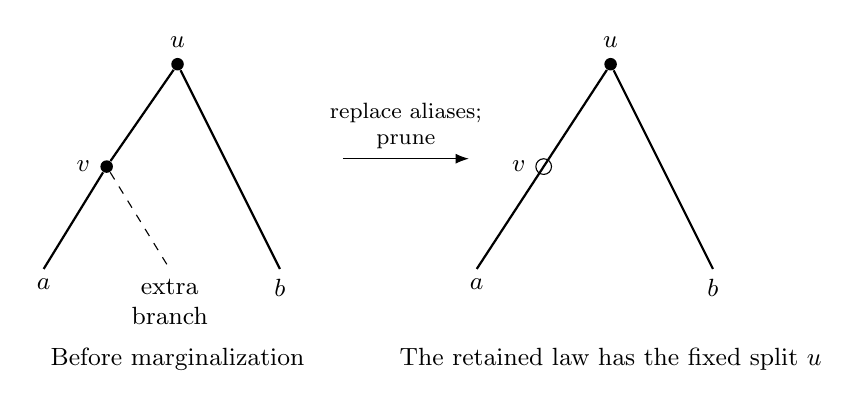
\begin{tikzpicture}[>=Latex,x=1cm,y=1cm,every node/.style={font=\small},dot/.style={circle,fill,inner sep=1.6pt}]
\node[dot,label=above:$u$] (u) at (0,2.6) {};
\node[dot,label=left:$v$] (v) at (-.9,1.3) {};
\coordinate (a) at (-1.7,0);
\coordinate (b) at (1.3,0);
\coordinate (q) at (-.1,0);
\draw[thick] (u)--(v)--(a) node[below] {$a$};
\draw[thick] (u)--(b) node[below] {$b$};
\draw[dashed] (v)--(q) node[below,align=center] {extra\\branch};
\node at (0,-1.15) {Before marginalization};
\draw[->] (2.1,1.4)--(3.7,1.4) node[midway,above,align=center,font=\footnotesize] {replace aliases;\\prune};
\node[dot,label=above:$u$] (u2) at (5.5,2.6) {};
\coordinate (a2) at (3.8,0);
\coordinate (b2) at (6.8,0);
\draw[thick] (u2)--(a2) node[below] {$a$};
\draw[thick] (u2)--(b2) node[below] {$b$};
\node[draw,circle,inner sep=2pt,label=left:$v$] at ($(u2)!.5!(a2)$) {};
\node at (5.5,-1.15) {The retained law has the fixed split $u$};
\end{tikzpicture}
\caption{The earlier-pair configuration in the centered integration argument. The pair $(a,b)$ splits at the fixed mass $u<v$. Replacing the aliases and integrating out the extra branch leaves the two paths on the right. Their joint law is independent of $v$, which now marks an evaluation point rather than a retained fork. Values at fixed projection cuts remain observables of these paths. The single-path estimate is applied under this fixed law before H\"older's inequality handles the other random factors.}
\label{fig:fixed-marginal}
\end{figure}


\Needspace{6\baselineskip}
\begin{proof}[Proof of Proposition~\ref{prop:statistics-high}]
\leavevmode\par
\paragraph{The covariance equation.}
Fix an old pair $ab$ splitting at or above $V_i$, where
$i\in\{1,2\}$, and put $P=Q_{ab}-S_{ab}$.  For every tested pair
$jk$ at or above the same threshold, define
\[
 u_{jk}=\nu[P(Q_{jk}-S_{jk})].
\]
These are pair functions on extensions of the old labels $ab$; unused
labels are ignored by marginalization.  Apply \eqref{eq:A7} at the
reference $K$, expanding $J=b\delta+bf+d$, where
$\delta=Q-S$.  Choose a fixed truncation degree large enough that
\eqref{eq:D11} makes the true Taylor remainder $O(x^K)$ for any needed
fixed $K$.  The row-deletion error remains $O(m^{-1})=O(x^6)$.
Every all-deterministic term vanishes against $P$.

Retain the high stochastic linear term on the left.  The equations
have the form
\[
 u_{jk}-\sum_{cd:\ v_{cd}\ge V_i}{\bf M}_{jk,cd}b_{cd}u_{cd}
       =R_{jk}^{\rm low}+R_{jk}^{\rm nonlinear}
                         +O(x^K)+O(x^6).
\]
The first source includes the stochastic linear term below $V_i$;
the second contains at least two insertions.  This left side is exactly
\eqref{eq:H1}, because the positive-law expectation of each inserted
pair with $P$ depends only on the indicated labels.  By \eqref{eq:P5},
its gap on retained levels is at least $c\lambda V_i^2$.  Proposition
\ref{inv:pair-inverse} therefore inverts it with cost $O(x^{-Ca_i})$,
once $p_*\ll a_i$ is chosen.  Evaluate the result at $jk=ab$.
The inverse adds only a bounded number of freely attached labels.
Their attachment densities and existing-fork weights are bounded after
removing the inverse cost; they do not turn a new low fork into a
prescribed atom.

As explained in the \hyperref[par:inverse-limits]{fixed-resolution limit argument}, these operations can first be made on resolutions keeping the tested cut and threshold. At fixed system size gaps persist on fine approximations; inverse domination with block restrictions allows replacing path expectations and coefficients outside that inverse by continuous-path ones with errors tending to zero (empty step intervals can be refined for attachment). Our bounds apply to bounded measurable topology weights from that inverse after its cost factor is removed.

Consider a nonlinear term containing a high stochastic
factor $\delta_{cd}$.  Keep $P$ and that factor untruncated.  There is
at least one further small factor: truncate it at $x^{\delta_*/2}$,
and bound all other factors uniformly.  Equation \eqref{eq:D11}
controls the discarded tails in arbitrarily high fixed moments.
Cauchy--Schwarz on the two untruncated factors gives
\[
 |\nu[P\delta_{cd}\,\hbox{remaining factors}]|
 \lesssim x^{\delta_*/2}\|P\|_2\|\delta_{cd}\|_2+O(x^K)
 \le x^{\delta_*/2}D_{ab}D_{H,i}+O(x^K).
\]
This preserves the exact second-moment factors; no higher norm
proportional to $D_{ab}$ is assumed.  Every remaining source contains
only low stochastic factors, so Lemma~\ref{lem:statistics-low-sources}
applies, including to the low linear term.

\paragraph{The coefficient of a sole low factor.}
If just one low insertion occurs at \(v\), its scalar coefficient indeed costs \(O(v)\): in every term of the finite quotient it belongs to a spin pair moment (possibly with other pairs), and all other pairs in that moment, including the tested pair if present, are high. Immediately across the low branching its two ends thus give two different groups of odd counts. Conditional on prefixes up to that cut, group expectations on independent continuations are odd smooth bounded functions (for the odd groups) with bounded gradients by the scalar source rules. Their product costs \(O(K(v))=O(v)\) using Brownian moments and bounded drift. More explicitly, the two odd group functions $F_1(z),F_2(z)$
vanish at zero and have uniformly bounded derivatives, so
$|F_1(z)F_2(z)|\le C|z|^2$.  The shared scalar prefix field at time
$K(v)$ has second moment $O(K(v))$ by its Brownian representation
with bounded drift.  Hence this scalar coefficient is $O(K(v))=O(v)$.
Additional labels and coincidences within the groups do not change
the odd parity or the derivative bound.

Combining these estimates after inversion gives
\begin{equation*}
 D_{ab}^2\lesssim_\diamond x^{-Ca_i}
       \bigl(x^{\delta_*/2}D_{ab}D_{H,i}
              +x^3\lambda^{-C}Z^2D_{ab}+x^6\bigr).
\end{equation*}
The final $x^6$ is the row-deletion contact error.  Increasing the
Taylor degree does not remove it.  Take the supremum over $ab$ and
write $D=D_{H,i}$.  Choose the power losses so that
$Cx^{\delta_*/2-Ca_i}<1/2$.  Absorption then leaves
\[
 D^2\lesssim_\diamond x^{3-Ca_i}\lambda^{-C}Z^2D
                         +x^{6-Ca_i}.
\]
If $D^2\le AD+B$ with $D\ge0$, then $D\le A+\sqrt B$ up to a fixed
constant.  Since $Z\ge1$ and $p_*\ll a_i$, the factors
$\lambda^{-C}$ and the permitted small losses can be included in a
fixed $C_Ha_i$.  This proves
$D_{H,i}\le x^{3-C_Ha_i}Z^2$ for $i=1,2$.

\paragraph{The longitudinal equation.}
For $r\ge V_1$, apply \eqref{eq:A7} without a random test.
The longitudinal identity \eqref{eq:H2} separates the linear term
into its diagonal and its integral part.  The resulting scalar equation
is
\[
 [1-b(r)\Gamma'(K(r))]f(r)
     =\Gamma'(K(r))d(r)+R_{\rm int}(r)+R_{\rm nonlinear}(r)+O(x^6).
\]
The diagonal is in field units; returning from normalized mass changes
only bounded constants.  Its lower bound is
\[
 1-b(r)\Gamma'(K(r))\ge c\lambda V_1^2.
\]
For the integral term, the post kernel bound in Section~\ref{sec:inverse}
gains the earlier time $K(u)\lesssim u$ when $u$ is small.  It gives
\[
 |R_{\rm int}(r)|\lesssim(1+M)^C\left(
       \int|d|\,du+\int_{u<V_0}u|f(u)|\,du
                          +\int_{u\ge V_0}|f(u)|\,du\right).
\]
The low dyadic envelope budget and the raw bound below $Y$ imply
$\int_{u<V_0}u|f(u)|du\lesssim_\diamond V_0Y^2$.
For the last integral use \eqref{eq:C2} and the majorant $Z_g$:
Cauchy--Schwarz, followed by a harmless weaker cutoff bound, gives
$\int_{u\ge V_0}|f(u)|du\lesssim
x^{2+c/2-a_0}Z_g$.  Thus the three terms on this right side are
\[
 O_\circ(x^3),\qquad
 O_\diamond(x^{2+a_0-p_*s_*}Z^2),\qquad
 O(x^{2+c/2-a_0}Z_g).
\]

For a nonlinear allocation with a factor at the prescribed fork $r$,
keep that factor and truncate one of the others at
$x^{\delta_*/2}$.  Its contribution is
\[
 O(x^{\delta_*/2})\bigl(|f(r)|+x^3+D_{H,1}\bigr).
\]
If no factor is pinned at $r$, integrate one factor in second norm.
The low envelope and the high comparison budget give
\[
 \int\|Q-q(u)\|_2\,du+\int|d(u)|\,du
 \lesssim_\diamond Y^2+x^{2+c/2-a_0}Z_g+x^3.
\]
A further factor contributes $x^{\delta_*/2}$ after truncation, even
when it is tied to the same vertex.  The negligible tails use a fixed
higher moment from \eqref{eq:D11}.

Divide by $c\lambda V_1^2$.  The coefficient of $|f(r)|$ is at most
$Cx^{\delta_*/2-p_*-2a_1}$, up to the fixed polynomial and small
power losses, and is absorbed.  The remaining leading exponents before
division are
\[
 3,\qquad 2+a_0-p_*s_*,\qquad
 2+c/2-a_0,\qquad 2+\delta_*/2-p_*s_*.
\]
The already proved variance bound controls the extra
$x^{\delta_*/2}D_{H,1}$ term.  Choose $a_0$ small relative to
$c,\delta_*$, then choose $b_H$ to be a sufficiently small fixed
fraction of $a_0$.  Next take $a_1$ sufficiently small, choose
$a_2\ll a_1$, and only then take $p_*$ sufficiently small that the
loss from the gap, $(1+M)^C$, and every permitted small power loss is
less than the remaining margins above $2+b_H$.
This also ensures $b_H\gg C_Ha_1$.  We obtain uniformly for $r\ge V_1$
\[
 |f(r)|\le x^{2+b_H}(Z^2+Z_g),
\]
as required.  This choice of $a_2\ll a_1$, followed by $p_*$,
preserves both this bound and the covariance absorption.
\end{proof}

\begin{remark}[The powers of the parameter majorants]\label{rem:statistics-majorants}
The parameter moment used throughout is $\mathbf E_\gamma Z^4\lesssim_\circ1$.
The direct construction uses $e=\min(r,Z^2\mathfrak h)$, whereas its
low-region size analogue incorporates $Y$ in the width and uses
$e=\min(r,\mathfrak h)$.  This is the reason for $Z_h=Z$ in the direct
integrated bounds and $Z_h=1$ in the low-region bounds: no extra power
of $Z$ is implicit in $\lesssim_\diamond$.  In particular the right side
of \eqref{eq:D8} is $x^{-C_0\delta'}z_1^0 U^2Z^4$ up to the permitted
losses.  The lower-band factor $Z^{7/4}$ is bounded by $Z^2$, and the
low-source and high-variance estimates require only $Z^2$.
The high-mean estimate additionally uses $Z_g$ with
$\mathbf E_\gamma Z_g^2\lesssim1$.  Hence the combinations needed later,
$Z^4$ and $Z_gZ^2$, are integrable by Cauchy--Schwarz.  These powers are
also valid for path parameters and site counts that vary measurably:
the majorants and all windows are chosen pointwise from deterministic
path data, before taking a positive-law expectation.
\end{remark}

\paragraph{Parameter order.}
The final-strength saving $c$ from \eqref{eq:C2} and the exponent $\delta_*$ in
\eqref{eq:D11} are fixed before the final choice of $p_*$.  Hence the row Taylor
degree in the covariance equation is fixed using $\delta_*$, and can
make the remainder, apart from $m^{-1}$ contacts, smaller than $x^6$ by
an arbitrary fixed power.  The inverse then has a fixed polynomial loss
in $(\lambda V_i^2)^{-1}$ and $1+M$.  Choose $a_0$ relative to
$c,\delta_*$, next $a_1$ relative to $a_0$, next $a_2$ relative to $a_1$,
and only then $p_*$ relative to all these gaps.  This gives
$b_H\gg C_Ha_1$ and $a_1\gg C_Ha_2$ without a degree depending on a later
choice of $p_*$.  The local strengthening depths and their power slacks
may then be fixed as in Section~\ref{sec:parameters}.  The geometric
loss exponent used in the width construction is chosen last, after the
finite moment and truncation orders have been specified.

\section{Finite pressure expansion and power count}\label{sec:expansion}

We now estimate the finite pressure polynomial that represents the
increment in Proposition~\ref{prop:increment}. The moment bounds control
its high-degree terms. For degrees two, three, and four, we must first
sum the signed scalar coefficients: the required saving appears only
after this sum and, on a size path, after applying the size derivative.

All estimates are on the stopped set. On direct strength paths we
restrict to \(Y\le x^\kappa\), since
Lemma~\ref{lem:statistics-coarse-switch} treats its complement. On size
paths we use the cap of Corollary~\ref{cor:statistics-cap}. Group masses
up to a fixed multiple of \(Y\) into one lower band, assigned scale
\(r=Y\), and use dyadic bands \(v\asymp r\) above it. Fixed changes in
these endpoints affect only constants. Write
\[
\delta=Q^*-S_v,\qquad f=S_v-q(v),\qquad \Delta=\delta+f.
\]
Here \(S_v\) is the untilted mean, used as the same deterministic
centering in both ensembles. When specified, \(Q^*\) is replaced by the
masked inner product of posterior means at a common later cut. The
allocation estimate below permits these projected factors. On size
paths we apply it only to factors in the low region of \eqref{eq:D2}.
The bounds on \(Q-q\) and \(S-q\) give the same envelope bound for
\(\delta\) by the triangle inequality; on the lower band it is \(O_p(Y)\).

\subsection{The pressure polynomial and its derivatives}

Choose a fixed Taylor degree \(J_0\), allowing different degrees for
size and direct variations. The size degree can be chosen from
\eqref{eq:D11} before any final decrease of \(p_*\). Take the size
stencil order at least this degree. Lemma~\ref{found:size-increment}
expresses the change from \(m\) to \(m+j\) as a polynomial in \(j\).
The stencil extracts its linear coefficient, which is the per-root
expectation of the whole symbol \eqref{eq:A6}. The path derivative
adds \(\partial_\theta\) of that symbol. Thus the operator for the size
increment is \({\cal O}=1+\partial_\theta\), with the unit acting on
every term. For a direct strength increment the operator is instead
\({\cal O}=\partial_{\log\lambda}\).

These operators act on formal polynomials: on a size path assign
\(\partial_\theta\Delta=-\Delta/6\), and on a direct path hold
\(\Delta\) fixed. This is the rule in Lemma~\ref{found:row-derivative},
not a derivative of a random overlap or of its law. Scalar coefficients
receive their ordinary parameter derivatives. After the exact
cancellation of the singleton cumulant with the linear counterterm,
\eqref{eq:A6} becomes, up to deterministic terms,
\[
 -\tfrac14\sum b\Delta^2+
 \sum_{j=2}^{J_0}\frac1{2^j j!}
   \sum_{\text{pairs}}\kappa_K(\tau_{a_1}\tau_{b_1},\ldots,\tau_{a_j}\tau_{b_j})
                 \prod_{i=1}^j (b\Delta+d)_{a_i b_i}.                \tag{E1}\label{eq:E3}
\]
where the pairs are ordered and off diagonal, and \(\kappa_K\) is their
joint scalar cumulant at fixed topology. We must bound the difference
of per-root positive-law expectations after applying \({\cal O}\) to
\eqref{eq:E3}. The degree counts below always refer to the base pair factors in this
polynomial. Coefficient differentiation may allocate an additional scalar
pair, whose clock weight is treated separately.

For high masses on size paths, \eqref{eq:D15} gives the needed gain.
For low masses, the remaining task is to obtain a coefficient of size
\(\lambda w^{5-j}\) for a product of \(j\) factors at scales at most
\(w\). This is why the next lemma uses that particular power of
\(w\). Its extra ratio for two distinct quadratic vertices records
the smaller split scale. We will obtain these coefficient bounds by
summing the signed scalar contributions of the polynomial; before doing
so, we prove the estimate that converts them into an increment bound.

\subsection{A centered allocation estimate}

\begin{lemma}[Centered allocation estimate]\label{exp:lem-centered-count}
Fix \(j\ge2\) pair factors. Each factor is either \(\delta\), possibly
projected, or a deterministic function bounded by
\(O_\diamond(e(v))\); use \(e=Y\) on the lower band. Fix the bands, their
order, and every projection cut. Each projection cut lies after the
split of its pair. Let \(s=1,\ldots,l\) index the distinct vertices to
which these factors are assigned, with multiplicities \(k_s\) and band
scales \(r_s\), and put \(w=\max_s r_s\). Suppose that the deterministic
weights are common to both ensembles and, on each of boundedly many
topology shapes, are bounded by
\[
 O_\diamond(\lambda w^{5-j})\ \prod_{s=1}^l dv_s/w,                    \tag{E2}\label{eq:E1}
\]
times measures of bounded volume in the other integration variables.
These are product majorants, so deterministic restrictions may be
retained. If \(j=l=2\), assume in addition the factor
\(O_\diamond(\min_s r_s/w)\). More explicitly, if \(H\) is this
deterministic weight and \(T_i^{\mathrm{tilt}},T_i^0\) are the pair
factors in the two ensembles, we estimate
\[
 \int H\left\{\nu^{\mathrm{tilt}}
       \left[\prod_{i=1}^jT_i^{\mathrm{tilt}}\right]
       -\nu^0\left[\prod_{i=1}^jT_i^0\right]\right\}.
\]
The weight, deterministic factors, cuts, and centering \(S\) are common;
only the positive law and the masked overlap vary. The absolute value
of this difference is bounded by
\[
 O_\diamond\big(\lambda Y^5(x/Y+g_B)\big)+O(x^K)                       \tag{E3}\label{eq:E2}
\]
where \(K\) can be arbitrarily large. Indeed the two contributions are
\[
 \lambda Y^5\frac{x}{Y}=x^5\lambda^{1-2s_*}Z^4,
 \qquad
 \lambda Y^5g_B=x^5\lambda^{(1-\eta)/2-s_*}Z^{7/2}.
\]
Both powers of \(\lambda\) are positive. Since
\(\mathbf E_\gamma Z^4\lesssim_\circ1\), the averaged bound is
\(O(x^{5+c'})\) for some \(c'>0\), after taking the allowed losses smaller
than these gains.
\end{lemma}

\begin{proof}
Set \(a_s=r_s/Y\), \(A=w/Y\), and \(m_{r_s}=Y/a_s\). The ratios
\(a_s\) and \(A\) are at least one. At a vertex carrying \(k\) factors,
\eqref{eq:D2} and the integrated envelope bound give
\[
 P_k=m_{r_s}^{\min(2,k)}r_s^{k-\min(2,k)}
\]
after integration in \(dv_s/r_s\). Thus one or two factors use the
first or second envelope moment, and each further factor costs \(r_s\).
Changing \(dv_s/w\) to \((r_s/w)dv_s/r_s\) in \eqref{eq:E1} shows that
the multiplier relative to \(\lambda Y^5\) is
\[
 F=A^{5-j-l}\prod a_s^{1+k_s-2\min(2,k_s)}
\]
with the additional factor \(\min_s a_s/A\) when \(j=l=2\).
The exponent of an individual \(a_s\) is \(0\) for a single factor,
\(-1\) for a double factor, and \(k_s-3\) for \(k_s\ge3\). Consequently
\[
\begin{array}{c|c}
\text{multiplicities}&F\text{ or an upper bound for }F\\ \hline
l=1&A\\
(1,2)&1/a_{\rm duplicate}\\
(1,1)&\min(a_1,a_2)\\
\text{all other cases with }l\ge2&A^{-1}.
\end{array}
\]
If an assigned vertex lies below \(x\), its integration uses only the
fraction \(x/Y\) of the lower band. In this case at least one \(a_s=1\),
and every entry in the table is at most a constant. Raw bounds in the
two ensembles therefore give the first contribution in \eqref{eq:E2}.

We may now assume that all assigned vertices are at least \(x\).
Fully deterministic products cancel, so there is a stochastic factor.
Suppose first that all stochastic factors occur at one vertex \(s\).
At that vertex, replace the overlaps by the common ancestor norm
squared and then by \(2L_v\) on a path through the fork. The alias
errors are controlled by \eqref{eq:D7}. Center the resulting polynomial
at its untilted expectation and apply \eqref{eq:D10}, treating the
other times and restrictions as deterministic coefficients. After
truncating the other factors at their envelopes, the cost is
\(O_\diamond(z_{r_s}^0r_sZ)\) times \(1\) for \(k_s=1\), or times
\(m_{r_s}r_s^{k_s-2}\) for \(k_s\ge2\). Relative to \(P_{k_s}\), this
gives at least the gain \(g_B/a_s\). On the lower band the same gain
follows from conditional averaging and the linear bound after
\eqref{eq:D9} when there is one stochastic power, and from the
integrated \(D_v^2\) bound when there are two or more. Multiplying by
the appropriate entry for \(F\) gives \(O_\diamond(g_B)\).

If stochastic factors occur at several vertices, select two of them
at scales \(aY,bY\). Their integrated second moments about \(S\), from
\eqref{eq:D7} and \eqref{eq:D9}, are bounded by
\(O_\diamond(g_BY^2/a)\) and \(O_\diamond(g_BY^2/b)\).
First apply unconditional Cauchy--Schwarz to the two selected stochastic
factors at fixed masses, and truncate the remaining factors at their
deterministic envelopes. At a selected vertex of scale \(r=aY\)
and multiplicity \(k\ge2\), Cauchy--Schwarz in mass then gives
\[
 \int e(v)^{k-1}D_v\,\frac{dv}{r}
 \lesssim r^{k-2}
    \left(\int e(v)^2\frac{dv}{r}\right)^{1/2}
    \left(\int D_v^2\frac{dv}{r}\right)^{1/2}
 \lesssim_\diamond r^{k-2}m_r
                 (g_BY^2/a)^{1/2}.
\]
Dividing by the raw budget \(P_k=m_r^2r^{k-2}\) gives the factor
\(O_\diamond(\sqrt{g_Ba})\); for \(k=1\), division of
\((\int D_v^2\,dv/r)^{1/2}\) by \(P_1=m_r\) gives the same
factor. Thus the two selected vertices improve the raw product by
\(O_\diamond(g_B\sqrt{ab})\). Since \(\sqrt{ab}\le A\),
this proves the claim whenever \(F\lesssim A^{-1}\).

There are two exceptional multiplicity patterns. For \((1,2)\), let
\(a_d\) be the duplicate scale and \(a_s\) the singleton scale. If both
factors at the duplicate are stochastic, selecting them uses
\(\int D_v^2\,dv/r\) at that vertex. Relative to its raw budget
\(m_r^2\), this gains \(O_\diamond(g_Ba_d)\), so
\(F g_Ba_d=g_B\). If only one is stochastic, selecting it together
with the singleton gives
\[
 Fg_B\sqrt{a_sa_d}=g_B\sqrt{a_s/a_d},
\]
which suffices when \(a_s\lesssim a_d\). In the remaining case the
later singleton is linear and stochastic. Integrating it as a centered
path integral gives \(g_B/A\), so the product with \(F=1/a_d\) is
again at most \(g_B\). For \((1,1)\), both factors must be stochastic.
The lower-band case has \(a_1=a_2=1\) and follows directly from
Cauchy--Schwarz. Otherwise the later linear factor has scale \(A\)
and gives \(g_B/A\); multiplying by
\(F=\min(a_1,a_2)\) gives at most \(g_B\).

For completeness, the last centered integration has a fixed marginal
law even though its fork moves. There is only one earlier stochastic
pair to retain. At most one of its leaves descends through the later
fork, so choose that leaf for the \(L\)-path when it is present. After
the alias replacement the other child of the moving fork has no
observable and integrates to one. The retained pair always splits at
its fixed earlier time. A prior projection merely evaluates these
same two paths at fixed later cuts. If neither endpoint descends
through the moving fork, choose a continuation whose separation from
the retained tree is at another fixed vertex. In either case the
moving time occurs only in the \(L\)-observable and in deterministic
kernels. Apply \eqref{eq:A2}, or its consequence \eqref{eq:D10},
unconditionally under this marginal and then apply H\"older with the
earlier random factor. This is the construction in
Remark~\ref{rem:statistics-earlier-pair}; it does not require an
inequality conditioned on that factor. Deterministic ties belong to
the kernels, and stochastic ties form one polynomial power. The
truncation and tilted-law transfers follow the conventions after
\eqref{eq:D10}. This proves \eqref{eq:E2}.
\end{proof}


\subsection{Taylor remainders and separation of the masses}

On size paths, \eqref{eq:D11} makes each insertion small in every fixed
moment. A sufficiently high fixed degree therefore bounds the Taylor
remainders using the absolute allocation measure. The differentiated
clock weights in \eqref{eq:A9} have absolute integrated norm
\(O_\circ(1)\). Their placements have bounded densities, including when
the added pair attaches to an existing integration variable; there is
no prescribed fork in this pressure calculation. Thus they cost only
a subpower factor.

The same weighted accounting applies to row contacts and normalization
errors. Since \(m\asymp N=x^{-6}\), their contribution is bounded by
\[
 O(m^{-1})\left(1+
   \|\dot b\|_{L^1}+\|\dot h\|_{L^1}
        +\|\dot K\|_{L^1}+\|\dot q\|_{L^1}\right)
       =O_\circ(x^6).
\]
Here the norms denote the absolute mass integrals with the
bounded-density allocation weights from \eqref{eq:A9}. The stencil
has finitely many fixed coefficients. Moreover,
Lemma~\ref{found:size-increment} gives a total-pressure remainder, so
no further factor \(m\) multiplies these errors. This proves that
\eqref{eq:A7}--\eqref{eq:A9} and the stencil reduce the size increment
to \eqref{eq:E3} with the required saving. On direct paths the
differentiated weights carry the additional factor
\(O_\circ(\lambda)\).

For a direct variation, start with the monotone reference
\(K_S=h+bS\). Apply \eqref{eq:A7} with insertions \(b\delta\), expanding
the pressure gradient of \eqref{eq:A9} through order \(J_0-1\).
By \eqref{eq:P8}, the test multiplying the cavity moment has degree
at most one and weight \(O_\circ(\lambda)\). In the true Taylor
remainder distinguish two cases. If at most one insertion has
\(e(v)\ge x^{\delta'}\), at least \(J_0-2\) insertions have smaller
envelope. Their moment bounds from \eqref{eq:D2} supply an arbitrarily
large fixed power of \(x\) once \(\delta'>0\) is fixed and \(J_0\) is
large enough. Choose the truncation losses first so that they do not
use up this gain.

If two insertions have \(e(v)\ge x^{\delta'}\), apply Cauchy--Schwarz
and \eqref{eq:D8} to those insertions, and bound the others uniformly.
The selected vertices have bounded absolute density even if the
insertions are tied. The one-row interpolated laws are comparable to
the genuine laws by \eqref{eq:A7}; the transfer to tilted active
components uses \eqref{eq:A4} and the stopping conventions after
Lemma~\ref{lem:statistics-centered}. Before averaging over \(\gamma\),
the cost is
\[
 O_\diamond\!\left(\lambda x^{-C_0\delta'}z_1^0Y^2Z^2\right)
 =O_\diamond\!\left(
 x^{5-C_0\delta'}\lambda^{(1-\eta)/2-s_*}Z^4\right).
\]
The fourth moment of \(Z\) therefore gives the averaged bound
\[
 O_\diamond(x^{5-C_0\delta'}\lambda^{(1-\eta)/2-s_*}),
\]
which saves a power when
\(C_0\delta'<p_*((1-\eta)/2-s_*)\), with room for the remaining
losses. We choose \(\delta'\) this small, also relative to \(\kappa\),
and then choose the direct Taylor degree.

Next expand the deterministic quotient coefficients from \(K\) to
\(K_S\), keeping the same total truncation degree. These scalar Taylor
remainders have bounded common coefficients and at least \(J_0\) pair
factors in all. Each factor is either \(K_S-K=bf+d\) or \(b\delta\).
Split the pressure-gradient test into its deterministic and linear
stochastic parts as well. We need only the difference between the two
ensembles, so Lemma~\ref{exp:lem-centered-count} applies once its
weight condition is checked. Every designated factor has its envelope
bound, and the density has prefactor \(\lambda\). With \(j\) factors
at \(l\) distinct vertices, changing to the normalized measure costs
\(w^l\). Since \(j+l\ge5\),
\[
 \prod_s dv_s=w^l\prod_s dv_s/w
       \lesssim w^{5-j}\prod_s dv_s/w.
\]
Thus the remainder has the weight \eqref{eq:E1} and is bounded by
\eqref{eq:E2}.

The retained terms recombine by Lemma~\ref{found:reference-change}.
Differentiating a scalar moment toward \(K_S\) inserts
\((K_S-K)\tau_a\tau_b/2\). Allocation symmetry permits these
insertions within products, with each scalar moment evaluated on its
own subtopology. Insertions into a unit moment sum to zero when
attached to the observed topology. Use these identities in the
unrestricted allocation sums, before dividing terms into mass bands
for estimates. The quotient retained through degree \(J_0-1\) is
therefore the quotient at \(K\) with argument
\(J=(K_S-K)+b\delta=b\Delta+d\).

By \eqref{eq:A9}, differentiating the logarithm through degree \(J_0\)
produces this gradient. Any additional highest-degree coefficient
derivatives have \(J_0\) factors and an \(O_\circ(\lambda)\) weight;
after splitting the factors into deterministic and stochastic parts,
the same calculation puts them in \eqref{eq:E1}. Pure deterministic
terms cancel. This establishes \eqref{eq:E3} on the whole remaining
direct path, including masses at which a pointwise small-insertion
argument was unavailable.

For size changes, first consider terms with a base pair at mass at
least \(V_2\). Call a base factor \emph{high} if its mass is at least
\(V_1\); recall that \(V_1<V_2\). Count the square term as two base
factors on the same pair. Expanding \(\Delta=f+\delta\), every high
deterministic factor, including \(d\) or \(\dot d\), is bounded by
\(O_\diamond(x^{2+b_H}(Z^2+Z_g))\). Stochastic high factors have the
variance bounds \eqref{eq:D15}; all factors also have the all-moment
smallness \eqref{eq:D11}. Low factors use their envelopes.

The scalar coefficients are bounded, including \(\dot b=O(1)\).
Differentiating \(K\) may add one scalar pair with weight
\(|\dot K|\). At high mass this weight is integrable separately. If
it is tied to a high base vertex, integrate against that same variable
and use the pointwise bounds \eqref{eq:D11}, \eqref{eq:D15}. At a low
mass \(v\), the inverse estimates give \(|\dot K(v)|=O(v)\).
The terms with at least one stochastic factor fall into the following
cases.
\begin{enumerate}
\item If there are two high stochastic factors, Cauchy--Schwarz gives
\(D_{H,1}^2\). If there is one high stochastic factor and a high
deterministic factor, the bound is
\(D_{H,1}x^{2+b_H}(Z^2+Z_g)\).
\item If every high factor is deterministic, extract the bound for
one of them and apply \eqref{eq:D16} to the low factors. A sole low
factor at \(v\) has the additional scalar coefficient \(O(v)\)
required there: immediately after its split, its two ends lie in
groups with odd parity, as in the proof of
Proposition~\ref{prop:statistics-high}. The square term cannot have
this configuration. An added dotted scalar pair preserves the
parity argument if it splits later than \(v\); if it splits earlier
or at \(v\), its own weight is \(O(v)\).
\item If a stochastic factor is the only high factor, it is the
factor at mass at least \(V_2\), so it costs \(D_{H,2}\). With one low
factor, the preceding parity argument gives
\(\int_{v<V_1}v e(v)\,dv\lesssim_\diamond V_1Y^2\). With two or more
low factors, integrate one using
\(\int e(v)\,dv\lesssim_\diamond Y^2\), and use \eqref{eq:D11} on
another to gain \(x^{\delta_*/2}\). Higher fixed moments and H\"older
give the same bound when these factors share a vertex.
\end{enumerate}
Here is the resulting power count, before \(\gamma\)-averaging and up
to the permitted losses. In the last two rows use
\(Y^2=x^2\lambda^{-s_*}Z^2\) and \(\lambda=x^{p_*}\).
\[
\begin{array}{l|l}
\text{selected factors}&\text{bound}\\ \hline
\text{two stochastic high}&x^{6-2C_Ha_1}Z^4\\
\text{stochastic and deterministic high}
 &x^{5+b_H-C_Ha_1}(Z^4+Z_gZ^2)\\
\text{only deterministic high}
 &x^{5+b_H-Cp_*}(Z^4+Z_gZ^2)\\
\text{sole stochastic high, one low}
 &x^{5+a_1-C_Ha_2-p_*s_*}Z^4\\
\text{sole stochastic high, two or more low}
 &x^{5+\delta_*/2-C_Ha_2-p_*s_*}Z^4.
\end{array}
\]
The hierarchy in \eqref{eq:D15} makes every exponent strictly larger
than five: it gives \(b_H\gg C_Ha_1\), \(a_1\gg C_Ha_2\), and permits
\(p_*\) to be chosen smaller than all remaining gaps. The factors
\(Z^4\) and \(Z_gZ^2\) have bounded \(\gamma\)-expectation, the latter
by Cauchy--Schwarz. Thus every displayed cost has the required
averaged saving. Products with no stochastic factor cancel outright.

On a direct path, terms whose maximum mass is bounded below by a
fixed positive constant already satisfy \eqref{eq:E1}. The dotted
weights supply \(O_\diamond(\lambda)\), and
\(|\dot d|\lesssim_\diamond\lambda r^2e\). For a quadratic term with
two distinct designated vertices, scalar parity gives the required
smaller-scale ratio. If differentiation adds a scalar pair at a
smaller mass \(v'\), its weight
\(|\partial_{\log\lambda}K(v')|\lesssim\lambda v'\) gives that ratio
instead.

All direct terms of degree \(j\ge5\) also satisfy \eqref{eq:E1} by
the normalized-measure calculation above. The same holds for the
remaining size terms of those degrees: now \(w\lesssim V_2\ll\lambda\)
and
\(\prod_s dv_s\lesssim\lambda w^{5-j}\prod_s dv_s/w\).
An extra dotted weight that is unbounded must be at a higher mass and
on a separate variable, where its absolute integral is available.
It remains to treat only low-region terms of degrees \(2,3,4\).

\begin{proposition}[Coefficients after compression]\label{exp:prop-low-coefficients}
Fix the dyadic restrictions on the base factors and a cut \(c\gg w\)
within the region where the small inverse is regular. A sufficiently
large fixed separation factor is enough; on size paths require also
\(c\lesssim\lambda\). Group base slots into blocks that share their
path through \(c\). Their split tree below \(c\) is the \emph{skeleton},
and every designated pair joins distinct blocks.

Apply the operator \({\cal O}\) defined above to the pressure
polynomial \eqref{eq:E3}: it is \(1+\partial_\theta\), with the
formal action \(\partial_\theta\Delta=-\Delta/6\), on a size path,
and \(\partial_{\log\lambda}\), holding \(\Delta\) fixed, on a
direct path. Group the resulting signed allocation coefficients by
this skeleton and sum their internal placements within each block.
The bound below concerns these differentiated, grouped coefficients.
This is a rearrangement of a signed measure. The probabilistic
expectations used to evaluate
the coefficients remain positive scalar laws on each fixed topology.
The spin-model pair tests have been projected to \(c\), or to a
neighboring smaller cut, so they depend only on the skeleton and can
be kept outside the internal sums. For \(j=2,3,4\), the resulting
coefficient, including the skeleton allocation weight, is bounded by
\[
 O_\diamond(\lambda c^{5-j})\prod_{s\ {\rm skeleton\ fork}} dv_s/c .       \tag{E4}\label{eq:E4}
\]
If \(j=2\), the designated vertices are distinct, and \(c\asymp w\),
the bound includes the further factor
\(O_\diamond(\min_s r_s/c)\). A factor \(d\) or \(\dot d\) may first
contribute \(\lambda c^2\) to the coefficient, leaving a deterministic
factor bounded by the ordinary envelope because \(r\lesssim c\).
Like \(b\) and \(\dot b\), these weights are constant during each
internal block sum.

Combine contributions only when they multiply the same product of
pair tests on the same skeleton. In particular, this combines a
repeated pair with the square counterterm. Give such terms the same
dyadic restrictions and projection cuts. The cut, shape, and mass
coordinates are fixed during coefficient differentiation. Internal
summation may then be done before or after that differentiation.
The spin tests receive only the formal action on \(\Delta\) already
specified: project the differentiated polynomial, without
differentiating a random test or a projection law.
\end{proposition}

\paragraph{Reduction to Proposition~\ref{exp:prop-low-coefficients}.}
Start with a sufficiently small fixed cut on direct paths, choosing
the low-mass threshold smaller still, and with a cut of order
\(\lambda\) on size paths. By
Corollary~\ref{cor:statistics-low-projection}, changing one pair to its
projection at \(c\) costs \(O_{p,\circ}(z_c^0c)\). Conditional on the
positive-law prefixes at that cut, a cross-block pair has exactly
its projected conditional mean. Expand a product as projected factors
plus changes. Terms with just one change have zero conditional mean,
so every error contains at least two changes.

For this first projection, bounded coefficient densities suffice.
Their prefactor is \(\lambda\) on direct paths and \(O_\circ(1)\),
including integrated dotted weights, on size paths. The respective
costs are \(O_\diamond(x^6\lambda^{-\eta})\) and
\(O_\diamond(x^6\lambda^{-C})\). Now reduce the cut by factors of two
until it is comparable to \(w\), retaining a large enough separation
factor. For a step from \(c\) to \(c/2\), first sum the coefficients
at \(c\) and apply \eqref{eq:E4}. The product error again contains at
least two changes of size \(O_{p,\circ}(z_c^0c)\); every other factor,
after extracting the defect weights allowed in the proposition, is
\(O_{p,\diamond}(c)\). Inactive masked pairs do not change. Hence the
step costs
\[
 O_\diamond(\lambda c^5(z_c^0)^2)
       =O_\diamond(x^6\lambda^{-\eta}/c)
       \lesssim_\diamond x^5\lambda^{s_*/2-\eta}
\]
because \(c\gtrsim Y\ge U\). At the final cut, \eqref{eq:E4} is
precisely \eqref{eq:E1}: the designated fork measures have the required
normalization, and the remaining skeleton variables have bounded
volumes in units of \(c\). Apply \eqref{eq:E2} to their expectation
difference. All cuts are common to the two ensembles. There are only
fixedly many degrees and shapes, and the dyadic bands and successive
cuts cost subpower factors. Thus Proposition~\ref{exp:prop-low-coefficients}
implies the remaining bounds for \eqref{eq:I}, uniformly also in the
site count, with a strict power saving.


\subsection{Scalar compression at a fixed cut}

\begin{proof}[Proof of Proposition~\ref{exp:prop-low-coefficients}]
We first evaluate the internal signed sum in \eqref{eq:E3} before
applying \({\cal O}\), and then justify commuting that operator with
the sum. Absolute values are taken only after the resulting
cancellations. Fix a cut \(c\) in the regular inverse region with
all designated pair splits strictly below it and
\(c\gtrsim w\ge Y\ge U\); on size paths also \(c\lesssim\lambda\).
Throughout coefficient differentiation, hold this cut, the skeleton
shape, its mass coordinates, and all mass restrictions fixed.

\paragraph{The objects in the compression formula.}
For a degree \(j\) term, partition its \(2j\) labeled endpoint slots
into blocks at \(c\). Let \(D\) be the number of blocks, ordered by
their first slots. The \(j\) ordered pairs form a graph on these
blocks; every edge has two distinct ends. The skeleton allocation
measure is the signed per-root measure for \(D\) ordered distinct end
labels in the hierarchy ending at \(c\), divided by \(c^D\).
Its absolute weight on each of finitely many shapes is bounded by
\[
 C_jc^{-1}\prod_{s\ {\rm skeleton\ fork}}dv_s/c.
\]
Indeed the first label has unit per-root weight, and each of the
remaining \(D-1\) placements contributes scale \(c\). Division by
\(c^D\) leaves \(c^{-1}\). After rescaling mass to \([0,1]\), the
remaining densities are bounded. Attachments at existing forks may
reuse their mass coordinates, but block identities remain distinct.
There are no prescribed old leaves or forks. Thus distinct free fork
coordinates are unequal almost everywhere, while a fork may have
more than two children.

Next let \(\pi\) be a partition of the \(j\) edges into cumulant
parts, keeping repeated edges as separately labeled slots. For a
part \(P\in\pi\), let \(k_{A,P}\) be the number of its endpoints in
block \(A\), and put
\[
 D_\pi=\sum_{P\in\pi}\#\{A:k_{A,P}>0\}.
\]
Thus \(D\) counts blocks in the full skeleton, whereas \(D_\pi\)
counts a block again each time it is used by another part. Neither
counts endpoint multiplicities.

On the fixed skeleton, let \(\zeta^A_u\), \(0\le u\le c\), be the
scalar prefix fields under the positive scalar law. They share their
Brownian driver until their skeleton separation, and thereafter use
independent transitions. Each part \(P\) uses a separate copy of this
law restricted to its blocks. The normalized source sum for \(k\)
slots inside one block is
\[
 s_k(z)=c^{-1}e^{-cV(t(c),z)}\partial_z^k e^{cV(t(c),z)}.
\]
With the explicit edge weights of \eqref{eq:E3} kept outside, the
coefficient multiplying the skeleton measure is
\[
 \sum_{\pi}(-1)^{|\pi|-1}(|\pi|-1)!\ c^{D_\pi}
       \prod_{P\in\pi}\mathbf E_{\rm low}
           \prod_{A\ {\rm in}\ P} s_{k_{A,P}}(\zeta^A_c).
                                                               \tag{E5}\label{eq:E5}
\]
The expectation \(\mathbf E_{\rm low}\) is probabilistic; the preceding
grouping of allocation coefficients by skeleton is a signed sum.

For example, take two copies of the edge \(AB\) between cut blocks.
Their original terminal labels may differ; projection makes their
spin-model pair tests identical. Abbreviate
\(s_1(\zeta^A_c)=\mathsf M_A\),
\(s_2(\zeta^A_c)=\mathsf P_A\). The one-part partition uses two
blocks, whereas the two-part partition uses each block twice. Their
combined internal coefficient is therefore
\[
 c^2\mathbf E_{\rm low}(\mathsf P_A\mathsf P_B)
   -c^4\bigl(\mathbf E_{\rm low}(\mathsf M_A\mathsf M_B)\bigr)^2.
\]
The skeleton measure contributes \(c^{-1}\), giving net powers
\(c\) and \(c^3\). There are two orientations of the second edge
for a fixed first edge, so its factor in \eqref{eq:E3} is
\(2/(2^2 2!)=1/4\). The square counterterm uses this same skeleton,
with internal coefficient \(c^2\) and weight \(-b/4\). These
normalizations will give the quadratic cancellation below.

\paragraph{The finite signed identity.}
First expand each cumulant into products of positive scalar moments
on its indicated edge sets. Once the skeleton assignments are fixed,
there is no restriction on the internal placements within a block.
A part observes only its own induced genealogy, so the internal
signed sums for different parts can be performed separately, even
when their actual terminal leaves coincide.

This factorization can be checked directly at finitely many levels
including \(c\). In the labeled product rule of
\cite[Proposition~2.5]{PE}, the coefficients choosing distinct children
are falling factorials of incoming-to-child mass ratios, and every
terminal source slot carries its terminal mass factor. Keep the
induced genealogies as discrete marks and first take the successive
ratios, including an auxiliary root ratio, to be sufficiently large
positive integers. The coefficients then count child identities.
After distinct block identities have been assigned at \(c\), the
choices for disjoint sets of slots inside a block are independent
counts, with terminal slots chosen with replacement. Their counts
therefore multiply. The resulting rational coefficient identity
extends by polynomial identity to the real masses, keeping terminal
mass fixed and dividing by the root mass before its zero limit.
This argument concerns only the coefficients; it does not extend
spin tests or probability laws from integer ratios.

\paragraph{Evaluation of the internal source sums.}
For one part, the positive scalar prefix law on its restricted
skeleton is independent of the internal placements after \(c\).
Conditional on these prefix fields, the source product rule sums
\(k\) internal slots in a block to
\(e^{-cV}\partial_z^k e^{cV}=c s_k\). Different blocks use independent
future kernels. Thus every used block contributes one factor \(c\),
giving \(c^{D_\pi}\), and the cumulant partition formula gives
\eqref{eq:E5}. Signed path limits and bounded fixed-order derivatives,
as supplied by PE, pass this finite-level identity to the continuous
paths. Equivalently, one may fix the prefix fields and approximate
only the future clocks within the blocks. There are no prescribed
internal split times to preserve in that approximation.

\paragraph{Differentiation at a fixed skeleton.}
The cut and skeleton measure stay fixed. Differentiating the scalar
moments adds one covariance pair with weight \(\dot K\). By
\eqref{eq:P8}, its absolute integrated weight is finite; its
non-atomic placements have bounded density for fixed cut and label
count. The same bound holds along affine comparison chords of the
clocks, so the finite signed differentiation rule and Fubini apply
to the internal sums.

To pass from chords to ordinary derivatives, fix \(N\). The
clock difference quotients are uniformly bounded in mass: for size
paths this follows from the smoothing floor and clipping, and for
direct paths from the localized smooth inverse perturbation. For
almost every parameter they converge at every mass in the low
region and at almost every other mass. The scalar kernels converge
by fixed-size path continuity. Dominated convergence therefore
passes the divided covariance insertions to the dotted insertions,
also for almost every fixed skeleton. A reused split is either one
of these integration coordinates or a prescribed low skeleton mass,
where convergence is pointwise; constant diagonals still cancel.
This proves that internal summation and a.e. coefficient
differentiation commute. We may choose the low-region partition
separately at each parameter when estimating the result: the
coefficient has already been differentiated, so no moving indicator
or cut is being differentiated.

\paragraph{Scalar jets and common-prefix estimates.}
Write
\(\chi=V_{zz}(0,0)\), \(g=V_{zzzz}(0,0)\),
\(k_0=t'(0+)>0\), and \(G(u,z)=V(t(u),z)\).
The notation \(O_*(A)\) controls both the value and the parameter
derivative: on size paths the derivative is \(\partial_\theta\),
and on direct paths it is \(\lambda^{-1}\partial_{\log\lambda}\).
The same convention applies to fixed \(L^p\) norms when fields are
coupled by common Brownian drivers in mass coordinates. Derivatives
of the explicit weights \(b,d\) will be handled separately.

By \eqref{eq:P1}--\eqref{eq:P2}, the inverse \(t\) is smooth here,
with \(t'\) bounded above and below and with the required higher
derivatives bounded. The positive-order spatial derivatives of \(G\)
also have bounded mass and spatial derivatives of every required
fixed order, allowing polynomial growth in \(z\) after parameter
differentiation. To see the mass derivatives, use
\[
 \partial_uG=-\tfrac12t'(G_{zz}+uG_z^2).
\]
For direct derivatives, differentiate the scalar PDE in \(\lambda\)
at fixed normalized time, as in the lift proof, and then compose with
the regular inverse. For size derivatives, use the rescaled scalar
jets, including the terminal-mass derivative already estimated in
Section~\ref{sec:paths}. These operations preserve evenness in the
field. In particular, on size paths,
\[
 \partial_\theta k_0=-3 k_0/6,\qquad
 \partial_\theta\chi=\chi/6+O(e^{-\Omega(M)}),\qquad
 \partial_\theta g=3g/6+O(e^{-\Omega(M)}).                              \tag{E6}\label{eq:E6}
\]
The normalized inverse slope and initial spatial derivatives are
constant under this rescaling, up to the exponentially small terminal
effect. This gives \eqref{eq:E6}. Moreover, \(\chi\) is uniformly
bounded above and away from zero. At every designated split,
\[
 b=b_\circ+O(\lambda c^2),\qquad b_\circ=\chi^{-2},
\]
and the error has the same bound under unscaled parameter
differentiation. By \eqref{eq:D2}, each \(d\) or \(\dot d\) can
likewise contribute \(O_\diamond(\lambda c^2)\) to the coefficient,
leaving its ordinary envelope factor.

The low prefix equation is
\[
 d\zeta=\sqrt{t'}\,dB+u t'G_z(u,\zeta)du.
\]
Starting from zero, this equation gives
\(\zeta_u=O_*(\sqrt u)\) and
\(\zeta_u-\sqrt{k_0}B_u=O_*(u^{3/2})\) in every fixed moment.
For a conditional evolution starting at \(z\), the field and its
parameter derivative have norms at most
\(C_p(|z|+\sqrt c)(1+|z|)^C\). Its spatial flow derivatives have
bounded moments, allowing polynomial growth in \(z\). These bounds
follow by differentiating the additive-noise equation: the drift is
smooth with bounded spatial derivatives, the differentiated
coefficients have polynomial growth, and each odd differentiated
drift vanishes at zero.

Evaluate the block observables at their fields at \(c\), unless
another time is specified. Taylor expansion, together with even/odd
parity and the definition of \(s_k\), gives
\[
\begin{split}
 \mathsf M_A := s_1(\zeta^A_c)&=G_z(c,\zeta^A_c)=\chi\zeta^A_c+O_*(c^{3/2}),\\
 \mathsf P_A:=s_2(\zeta^A_c)&=G_{zz}(c,\zeta^A_c)+c(G_z(c,\zeta^A_c))^2
                        =\chi+O_*(c),\\
 s_3(\zeta^A_c)&=g\zeta^A_c+O_*(c^{3/2}),\qquad
 s_4(\zeta^A_c)=g+O_*(c).
\end{split}                                                            \tag{E7}\label{eq:E7}
\]
For blocks \(A,B\) splitting at \(v_{AB}<c\), the martingale
property of \(G_z\) reduces their product expectation to the common
prefix at \(v_{AB}\). Thus
\[
 \mathbf E_{\rm low} \mathsf M_A\mathsf M_B=\chi^2 k_0 v_{AB}+O_*(v_{AB}^2).
\]
We also need
\[
 \mathbf E_{\rm low} \mathsf P_A\mathsf P_B
   =\chi^2+\chi^3 k_0 c^2+\tfrac12 g^2 k_0^2 v_{AB}^2+O_*(c^3).       \tag{E8}\label{eq:E8}
\]
To obtain \eqref{eq:E8}, keep the terminal cut \(c\) fixed and set
\(H_u=G_{zz}(u,\zeta_u)+cG_z(u,\zeta_u)^2\). The PDE and It\^o's
formula give drift \((c-u)t'G_{zz}^2\) and diffusion coefficient
\(\sqrt{t'}(G_{zzz}+2cG_zG_{zz})\). In the product of the two block
processes, the two drift integrals sum to
\(\chi^3k_0c^2+O_*(c^3)\), by \eqref{eq:E7}. Their common quadratic
variation stops at \(v_{AB}\); its expected rate before that time is
\(g^2k_0^2u+O_*(cu)\). Its integral is the term
\(\tfrac12g^2k_0^2v_{AB}^2\), with an error of order \(O_*(c^3)\).

For three blocks we use
\[
 \mathbf E_{\rm low} \mathsf P_A \mathsf M_B\mathsf M_C=\chi^3 k_0 v_{BC}+O_*(c^2).
                                                                        \tag{E9}\label{eq:E9}
\]
When the designated splits are distinct, this estimate retains the
earlier mass. Suppose \(v_{AB}=h'<v_{AC}\), so that \(v_{BC}=h'\).
Condition at \(h'\) on the common field \(z\). After subtracting
\(\chi\mathsf M_B\mathsf M_C\), the conditional expectation on the
\(A,C\) side is that of \((\mathsf P_A-\chi)\mathsf M_C\). It is an
odd function of \(z\), with spatial derivative bounded by
\(C(c+z^2)(1+|z|)^C\), also after parameter differentiation at fixed
\(z\). Indeed \(\mathsf P-\chi=O(c+|\zeta_c|^2)\), its spatial
derivative is \(O(|\zeta_c|)\), and \(\mathsf M=O(|\zeta_c|)\)
with bounded derivative; apply the conditional flow bounds and
H\"older to their product.

The \(B\)-side conditional mean is \(G_z(h',z)\), of size
\(O_*(|z|(1+|z|)^C)\). Substituting the common prefix field
\(z=O_*(\sqrt{h'})\) therefore bounds the error in \eqref{eq:E9}
by \(O_*(ch')\). The other ordering is identical after exchanging
\(B,C\). Without a designated earlier split, \eqref{eq:E7} gives
the stated \(O_*(c^2)\) error.

\paragraph{The coefficients canceled by size rescaling.}
For a pure degree \(j\) term with no defect factors, the formal
rule \(\partial_\theta\Delta=-\Delta/6\) makes the size operator on
its coefficient equal to \(1-j/6+\partial_\theta\). Since
\(\ell=e^{\theta/6}\),
\[
 \left(1-\frac j6+\partial_\theta\right)
       \ell^{-(6-j)}=0.
\]
Equation~\eqref{eq:E6} and \(b_\circ=\chi^{-2}\) identify exactly
the coefficients with this scaling:
\[
\begin{array}{c|c|c}
 j&\text{coefficient monomials}&\text{size scaling}\\ \hline
 2&b_\circ^2\chi^3k_0,\quad b_\circ^2g^2k_0^2&\ell^{-4}\\
 3&b_\circ^3g^2k_0,\quad b_\circ^3\chi^3&\ell^{-3}\\
 4&b_\circ^4g^2&\ell^{-2}.
\end{array}
\]
The masses multiplying these monomials are held fixed. Exponentially
small terminal errors will be retained until the end. On direct
paths, the operator is only \(\partial_{\log\lambda}\), and the
\(O_*\) convention already supplies the factor \(\lambda\).
For a term with a defect, use the product rule and extract at least
one factor \(\lambda c^2\) as above. In the remaining case analysis
we include the net factor \(c^{D_\pi-1}\); the normalized skeleton
fork measure in \eqref{eq:E4} is left outside.

\Needspace{8\baselineskip}
\paragraph{The low-degree cases.}
\begin{enumerate}
\item Suppose \(j=2\) and \(D=2\). The two edges join the same
blocks, so use the repeated-edge calculation following \eqref{eq:E5}.
Its coefficient combines with the square counterterm because both
multiply the same projected pair square. After extracting the common
skeleton measure and \(c^2/4\), their coefficient before
differentiation is
\[
 b^2\left\{\mathbf E_{\rm low}\mathsf P_A\mathsf P_B
       -c^2(\mathbf E_{\rm low}\mathsf M_A\mathsf M_B)^2\right\}-b.
\]
The constant term \(b^2\chi^2-b\), and its unscaled derivatives, are
\(O(\lambda c^2)\) because \(b_\circ\chi^2=1\) and
\(b-b_\circ=O(\lambda c^2)\). The next two terms from \eqref{eq:E8},
after replacing \(b\) by \(b_\circ\), are
\[
 b_\circ^2\chi^3k_0c^2,
 \qquad \tfrac12b_\circ^2g^2k_0^2v_{AB}^2.
\]
Their direct derivatives are \(O(\lambda c^2)\); their size
contributions cancel by the \(j=2\) row of the table. Substitution
errors from \(b-b_\circ\) have the required bound. The remaining
\(O_*(c^3)\) errors, including the smaller product-of-means term,
contribute \(O(c^4)\) after the net compression factor \(c\).
On size paths this is \(O(\lambda c^3)\) because \(c\lesssim\lambda\);
on direct paths the derivative supplies \(\lambda\) itself.
Thus \eqref{eq:E4} holds. A defect factor supplies
\(\lambda c^2\) directly and gives the same bound, with the allowed
\(O_\diamond(1)\) loss.

\item Suppose \(j=2\) and \(D=3\), with edges \(AB,AC\).
For the one-part partition, \eqref{eq:E9} gives the leading
coefficient \(b_\circ^2\chi^3k_0v_{BC}\), with net compression
factor \(c^2\). Its size contribution cancels by the same row of
the table; its direct derivative costs \(O(\lambda c^3)\), or
\(O(\lambda c^2h')\) when \(v_{BC}=h'\) is the earlier split.
The error is \(O_*(c^2)\), or \(O_*(ch')\) when the designated
vertices are distinct and their earlier mass is \(h'\).
Multiplication by \(c^2\), followed on size paths by
\(c\lesssim\lambda\), gives respectively
\(O(\lambda c^3)\) and \(O(\lambda c^2h')\). The errors from
\(b-b_\circ\) and any defect factors satisfy these same bounds.
For the two-part partition the product of pair moments is
\(O_*(v_{AB}v_{AC})\), with net factor \(c^3\), which is smaller
still. Since \(h'\lesssim\min_s r_s\), the refined bound gives the
extra ratio required in \eqref{eq:E4}.

\item Suppose \(j=2\) and \(D=4\). Both partitions have net
factor \(c^3\), and their products of moments are \(O_*(c^2)\).
When the designated vertices are distinct with earlier mass \(h'\),
these products are also \(O_*(h')\). For a product of two pair
moments this follows at once from their individual bounds. For the
four-spin moment, condition on the prefixes at \(h'\). The earlier
edge has separated ends, while the ends of the later edge are still
together. Hence at least two of the independent future groups have
odd parity. Each such group's conditional expectation vanishes at
zero starting field and has a polynomially bounded spatial
derivative, also after parameter differentiation. The common prefix
fields have size \(O_*(\sqrt{h'})\), so the product of these two
odd expectations gives \(O_*(h')\).

On size paths the refined contribution is therefore
\(O(c^3h')\le O(\lambda c^2h')\), exactly the required smaller-scale
bound. On direct paths the derivative supplies \(\lambda\).
The unrefined \(O_*(c^2)\) estimate gives \eqref{eq:E4} without the
ratio. Extracting defect factors preserves both conclusions.

\item Suppose \(j=3\), for which the target is
\(O_\diamond(\lambda c^2)\). Terms with defects or with
\(D_\pi\ge4\) already have enough powers of \(c\): on a size
path one extra power is bounded by \(\lambda\), and on a direct
path the derivative supplies \(\lambda\). It remains to consider
one-part partitions with two or three blocks.
For \(D=2\), each block has degree three and \eqref{eq:E7} gives
\(g^2k_0v_{AB}+O_*(c^2)\). For \(D=3\), an odd block degree gives
\(O_*(c)\); otherwise all three degrees are two, giving
\(\chi^3+O_*(c)\). The two leading monomials after multiplication
by \(b_\circ^3\) are precisely those in the \(j=3\) row of the
table, so their size contributions cancel. With net factors \(c\)
and \(c^2\), respectively, the remaining errors are \(O(c^3)\),
which is at most \(O(\lambda c^2)\). Direct derivatives give the
same target without this cancellation.

\item Suppose \(j=4\), for which the target is
\(O_\diamond(\lambda c)\). Only size terms with no defect and
\(D_\pi=2\) lack the required power before cancellation. Such a
term has one part, on two blocks of degree four each. Its moment is
\(g^2+O_*(c)\). Multiplication by \(b_\circ^4\) gives the last
row of the table, so the leading size contribution cancels. The
remainder with net factor \(c\) is \(O(c^2)\), at most
\(O(\lambda c)\). All other terms have an additional compression
power, a defect factor, or the direct derivative factor
\(\lambda\).
\end{enumerate}
The exponentially small terminal errors retain the mass factors of
their corresponding main terms. Since \(M=\log^3(1/x)\), they are
smaller than every fixed power of \(x\). This proves \eqref{eq:E4}.
\end{proof}

The row expansion, the high-mass estimates, and the low-degree
coefficient bound now give both increments required in
Proposition~\ref{prop:increment}. The final parameter choice in
Section~\ref{sec:parameters} makes their savings simultaneous and
justifies the stated uniformity for moving site weights.

\section{Parameter choices and completion of the proof}\label{sec:parameters}

Recall that \(x=N^{-1/6}\) and
\(x^{12}\le\lambda\le x^{p_*}\).  The parameters below are fixed
independently of \(N\).  We first choose the savings used to control
size changes, then the final-strength exponent \(p_*\), and only then
the truncation and loss parameters for direct changes. The essential
order is that the size Taylor degrees determine the polynomial loss
constants before the cutoffs and \(p_*\) are selected. Direct Taylor
degrees may be larger, because their estimates do not enter that size
choice. Every degree, moment order, and loss exponent below is fixed
before \(N\to\infty\).

\begin{enumerate}
\item Fix \(T>1\) and the neighborhoods, tapers, and constants
\(c_1,c_b\) in \eqref{eq:P1}--\eqref{eq:P7}, leaving strict room in
the admissibility and derivative bounds.  The global saving \(c_G\)
in \eqref{eq:G1} is available before choosing \(s_*\) near \(1/2\)
or the ultimate small \(p_*\).  In its proof, the coarse clock estimate
\eqref{eq:G3} supplies a fixed saving first.  Choose \(a_g\) below
that saving, then \(d_g\) small enough to absorb the fixed
inverse-kernel loss in the covariance estimate following
\eqref{eq:G4}, and finally the PE power slack
for this global comparison small relative to \(d_g\).  The endpoint
condition \eqref{eq:P9} uses the common base temperature as explained
in Section~\ref{sec:global}.  It requires \(\lambda\to0\), without
requiring \(\lambda\le x^{a_g}\).  Thus later decreases of \(p_*\)
do not decrease \(c_G\).

\item Set \(k_c=0.03\).  Choose
\(\tau\ll\min(10^{-4},c_G)\), put \(s_*=1/2-\tau\), and then
choose \(\eta\ll\tau\) and \(\tau_0\ll\eta\), with
\(s_0=s_*-\tau_0\), as in \eqref{eq:C1}--\eqref{eq:C2}.
Choose \(b_s>0\) so that
\[
 2(\tau+\tau_0)+b_s<\min(c_G/12,k_c/3),\qquad
 b_s<2(\eta-\tau_0),
\]
and then \(b_\ell\ll b_s\).  These inequalities leave room for the
local comparison errors throughout \(\lambda\ge x^{12}\).
Choose also \(h_e\ll\min(1,c_G)\).

Both final-strength estimates in \eqref{eq:C2} now have a fixed
saving \(c>0\) for every sufficiently small \(p_*\).  Indeed, with
\(\lambda=x^{p_*}\), \(U=x\lambda^{-s_*/2}\), and the edge seed
off, the differentiated bound in its proof has powers
\[
 4+c_G-p_*,\qquad 5+p_*(2\eta-5s_*/2),\qquad 6-2p_*.
\]
All remain separated above \(4\) as \(p_*\) decreases.  The
smoothing error \(O(x^{5+c'})\) in \eqref{eq:P11}, divided by
\(\lambda\), has exponent \(5+c'-p_*>4\) as well.
Likewise \eqref{eq:D11} supplies a fixed
\(\delta_*>0\), for example \((1/200)/50\), under the preliminary
restriction \(p_*<(1/200)/100\).  Neither saving depends on the
remaining choice of \(p_*\).

\item Fix the size row and pressure Taylor degrees using
\(\delta_*\).  In the covariance equation proving \eqref{eq:D15},
choose the row degree so that the Taylor remainder before inversion,
apart from the \(O(m^{-1})\) contacts, is smaller than \(x^6\) by
a fixed power.  This is possible by \eqref{eq:D11} and requires no
further information about \(p_*\).  For these fixed degrees the
inverse has fixed polynomial losses in
\((\lambda V_i^2)^{-1}\) and \(1+M\); the low sources have a fixed
loss \(\lambda^{-C}\).  Fix constants bounding these losses before
choosing the cutoffs, large enough to cover all the estimates below.

Now choose \(a_0\) small relative to \(c,\delta_*\), take \(b_H\)
to be a sufficiently small fixed fraction of \(a_0\), then choose
\(a_1\) small relative to \(a_0,b_H\), and \(a_2\) small relative
to \(a_1\).  Finally choose \(p_*\) small relative to these gaps and
to \(h_e\), including the restriction needed for the cap on \(Y\)
after \eqref{eq:D11}.  With \(V_i=x^{a_i}\), the high-mass terms
of \eqref{eq:E3} then have the following positive margins over
\(x^5\):
\[
\begin{gathered}
 1-2C_Ha_1>0,\qquad b_H-C_Ha_1>0,\qquad b_H-Cp_*>0,\\
 a_1-C_Ha_2-p_*s_*>0,\qquad
 \delta_*/2-C_Ha_2-p_*s_*>0.
\end{gathered}
\]
The first two margins cover two high stochastic factors and a high
stochastic factor paired with a high deterministic factor.  The third
covers a high deterministic factor times the low-source estimate
\eqref{eq:D16}.  The last two cover a sole high stochastic factor,
using respectively the parity-weighted integral \(V_1Y^2\) or a
further factor \(x^{\delta_*/2}Y^2\).  In both cases
\(Y^2=x^2\lambda^{-s_*}Z^2\).  The size projection errors
\(x^6\lambda^{-C}=x^{6-Cp_*}\) also have the positive margin
\(1-Cp_*\).  No subsequent step decreases \(p_*\).

\item Fix the number of strengthening stages in \eqref{eq:C11}.
Choose \(\zeta\) small relative to the power margins in
Section~\ref{sec:budgets}; in particular, it is smaller than \(p_*\)
times each required gap in a \(\lambda\)-exponent, including the gaps
involving \(b_\ell\) and \(\tau_0\).  Then choose the local PE
power slacks small relative to \(\zeta\), and the buffer exponent
\(\rho\) small enough for \eqref{eq:C18}.  The remaining finite
profile and moment iterations, and their subpower losses, can be
chosen with these parameters fixed.

The extra optimized excess
\(O(x^{4-2\zeta}u\Lambda^{1/3})\) fits the budget at
\eqref{eq:C3}: after division by \(\lambda u\), its ratio to
\(x^4\lambda^{-2s_0}\) is
\(x^{-2\zeta}\lambda^{k_c/3-1+2s_0}\), which is power small by
these choices.  The final-strength switch error
\(O(x^{5+c'})\) from \eqref{eq:P11} also fits after division by
\(\lambda u\).  At the smallest dyad \(u\asymp U\), its ratio
to \(U^4\) is at most
\(x^{c'}\lambda^{5s_*/2-1}\); larger dyads improve this bound.
Both exponents are positive, so the switch leaves room for the
remaining losses.

\item For the direct paths, choose the coarse cutoff exponent
\(\kappa>0\) small relative to the gains in
Lemma~\ref{lem:statistics-coarse-switch}.  More precisely, its
large-\(Y\) event costs \(x^{-4\kappa}\), so choose
\[
 4\kappa<\min\left\{p_*(1-2s_*),\,
                       (1-\eta)/s_*-2\right\}.
\]
Both quantities on the right are positive by the choices of
\(s_*,\eta\).  The gains used in the
remaining direct expansion are
\[
 1-2s_*=2\tau>0,\qquad
 (1-\eta)/2-s_*=\tau-\eta/2>0,\qquad
 s_*/2-\eta>0.
\]
A factor \(\lambda^g\) with any of these exponents \(g>0\) is at
most \(x^{p_*g}\).  Choose \(\delta'>0\) smaller than \(\kappa\)
and small enough that
\[
 C_0\delta'<p_*\bigl((1-\eta)/2-s_*\bigr),
\]
with strict room for the later losses.  Thus the direct Taylor error
\(x^{5-C_0\delta'}\lambda^{(1-\eta)/2-s_*}\) saves a power over
\(x^5\).  Now fix the direct pressure Taylor degree large enough
also for this \(\delta'\).  The initial direct projection cost
satisfies
\(x^6\lambda^{-\eta}\le x^{6-12\eta}\), so its margin over
\(x^5\) is \(1-12\eta>0\).

Choose the fixed moment and change-of-measure orders large enough
that truncation and transfer lose only small fractions of the margins
just retained.  Then choose the geometric loss in \eqref{eq:D1} and
\eqref{eq:D10}, and the subpower losses, still smaller.  The smooth
density comparisons on intervals of length \(O(b_\epsilon)\) may
require higher fixed orders after this geometric choice; they change
constants only.  Finally take the stencil order large enough for
both the fixed size pressure polynomial and the site-weight smoothing
in Section~\ref{sec:reduction}.  Enlarging this order does not require
enlarging the size Taylor degree.
\end{enumerate}

These choices give a common positive saving in the stopped increment
bounds.  For a direct strength sweep, Lemma~\ref{lem:statistics-coarse-switch}
handles \(Y>x^\kappa\); on the complement apply the allocation
and compression estimates \eqref{eq:E2}, \eqref{eq:E4} to the
pressure polynomial \eqref{eq:E3}. The two multiplier sweeps use the
separate switch bounds of the same lemma. The size sweep uses the
capped low statistics, \eqref{eq:D15}, and the size versions of these
polynomial estimates.  Integrating the direct strength
parameter costs only \(O(\log(1/x))\).  The size segment has bounded
length, and the multiplier bound has at most the integrable endpoint
factor \(\chi_e^{-1/2}\).  The fixed-degree dyadic and projection-cut
sums cost subpower factors.  Decreasing the common saving absorbs
these integration and summation costs.

We spell out the uniformity needed when the site count varies.  At
each fixed size-path point \(\theta\), every estimate above is
applied to the particular integer \(m\) being tested, uniformly for
\(N/2\le m\le3N\).  In particular, the averaging in
\eqref{eq:C1}--\eqref{eq:C2} is over \(\gamma\) at this fixed
\((\theta,m)\).  The physical clocks are common to these site
counts.  Their absolute dotted-clock norms are bounded up to subpower
loss as explained after \eqref{eq:P8}; integrating any remaining
dotted weight in mass therefore gives a common integrable envelope
in \(\theta\).  Thus the bound is uniform in \(m\) before
integrating \(\theta\).

Let \(w_m(\theta)\ge0\) be measurable probability weights on the
allowed integers.  Multiplying the parameter-averaged bound at
\((\theta,m)\) by \(w_m(\theta)\) and summing preserves its
common envelope, since \(\sum_m w_m(\theta)=1\).  A measurable
choice of a single \(m(\theta)\) is the special case of a point
mass.  Fixed-size path approximation makes the pressure tests and
statistics measurable, and absolute continuity supplies their a.e.
path derivatives.  Fubini first removes a null set of \(\theta\)
for each parameter-averaged estimate.  At fixed \(N\) there are only
finitely many allowed \(m\), so their exceptional sets can then be
united into one null set before weighting and integrating.

For each summand the change of measure is used only on the central
stop \(\mathcal K_m(s)\le3x^\varepsilon\).  The comparisons with
finitely many added rows in \eqref{eq:A6}--\eqref{eq:A9} have bounded
covariance changes and estimate their remainders with moments of the
original \(m\)-site system.  They therefore require this same stop,
without a new stopping condition for the added-row systems.  Fix the
common saving before taking the small Laplace exponent
\(\varepsilon\) in Section~\ref{sec:reduction}; this exponent is
distinct from the geometric slack. The density bounds on the stop hold
for every fixed finite order, so they cover all transfer orders chosen
above, for every sufficiently small fixed \(\varepsilon>0\) and each
fixed test coefficient \(q>0\) in \(s=qx^{1+\varepsilon}\).

For one such test, the same parameter bounds cover the finitely many
segments in the comparison from \(N\) to any \(N'\in[N,2N]\).
Summing their stopped bounds and then choosing \(\gamma\) gives the
single route used in Section~\ref{sec:reduction}. Different tests may
choose different routes: their bare endpoint laws are independent of
\(\gamma\). Thus the later interpolation at finitely many Laplace
tests requires no parameter choice uniform over an infinite test family.

This proves Proposition~\ref{prop:increment}, including its version
with a measurably varying site count or site weights.
Section~\ref{sec:reduction} then proves Theorem~\ref{thm:moments}
and proves Proposition~\ref{def:law}.  Removing the independent
Gaussian completion and dividing by the exact finite-size standard
deviation, as done there, proves Theorem~\ref{thm:main} for every
fixed \(\beta>1\).

\section{Proofs of the fluctuation and disorder-chaos corollaries}
\label{sec:consequences}

The two consequences in the introduction now follow from the main
variance asymptotic and existing comparison inequalities. We keep the
finite-size normalizations explicit.

\subsection{The SK--Curie--Weiss comparison}

\begin{proof}[Proof of Corollary~\ref{cor:skcw}]
Abbreviate $F_n^{\mathrm{CW}}=F_n^{\mathrm{CW}}(\beta,\gamma)$ and
couple it with $F_n(\beta)$ using the same disorder. For
$\Delta_n=F_n^{\mathrm{CW}}-F_n(\beta)$, \cite[Proposition~1.5]{DeyKang2026} gives
$\Delta_n\ge0$ and, for every $u\ge0$ and $n$,
\[
 \mathbb P(\Delta_n\ge u)\le C_\gamma e^{-u},
 \qquad C_\gamma=(1-\gamma)^{-1/2}.
\]
Integrating the tail yields the uniform bounds
\[
 \begin{gathered}
 \mathbb E\Delta_n^2
 =2\int_0^\infty u\,\mathbb P(\Delta_n>u)\,du
 \le2C_\gamma,\\
 \|\Delta_n-\mathbb E\Delta_n\|_2
 \le K_\gamma:=\sqrt{2C_\gamma}.
 \end{gathered}
\]
In particular the perturbed mean and variance are finite. Let
$t_n=\sqrt{\Var F_n^{\mathrm{CW}}}$. The reverse triangle inequality
in $L^2$ gives
\[
 |t_n-s_n(\beta)|
 \le\|\Delta_n-\mathbb E\Delta_n\|_2\le K_\gamma.
\]
Since $s_n(\beta)\sim\sqrt{a_2(\beta)}n^{1/6}\to\infty$, we have
$t_n/s_n(\beta)\to1$, which proves the variance asymptotic and makes
$t_n$ positive for all sufficiently large $n$. For those $n$, using
$\|X_n(\beta)\|_2=1$,
\[
 \left\|\frac{F_n^{\mathrm{CW}}-\mathbb E F_n^{\mathrm{CW}}}{t_n}
             -X_n(\beta)\right\|_2
 \le\frac{K_\gamma}{t_n}
   +\left|\frac{s_n(\beta)}{t_n}-1\right|
 \le\frac{2K_\gamma}{t_n}\longrightarrow0.
\]
Theorem~\ref{thm:main} and Slutsky's theorem now give the asserted law.
\end{proof}

\subsection{Disorder chaos in the zero-field model}

\begin{proof}[Proof of Corollary~\ref{cor:disorder-chaos}]
For the Gaussian field in \eqref{eq:model},
\[
 \rho(\sigma,\tau):=\Cov(H_n(\sigma),H_n(\tau))
 =\frac1n\sum_{i<j}(\sigma_i\tau_i)(\sigma_j\tau_j)
 =\frac{nR^2-1}{2}.
\]
Writing a single subscript for one Gibbs average, set
\[
 q(t)=\mathbb E\langle\rho\rangle_{g,g^t}
 =\frac1n\sum_{i<j}
 \mathbb E\big[\langle\sigma_i\sigma_j\rangle_g
               \langle\sigma_i\sigma_j\rangle_{g^t}\big].
\]
These Gibbs means are smooth with all derivatives bounded. Applying
\cite[Lemma~3.3]{Chatterjee2009} to them at its two-sided time $t/2$
shows that $q$ is nonnegative and nonincreasing. The variance identity
\cite[Theorem~3.8]{Chatterjee2009}, applied to $F_n/\beta$, gives
\[
 \frac{\Var F_n(\beta)}{\beta^2}
 =\int_0^\infty e^{-s}q(s)\,ds
 \ge (1-e^{-t})q(t).
\]
Since $q(t)=(n\mathbb E\langle R^2\rangle_{g,g^t}-1)/2$, this proves
\eqref{eq:chaos-ou}.

For replacement, apply \cite[Theorem~3.14]{Chatterjee2009} directly to
the $M$ independent coordinates, regarding
$f=F_n(\beta)/(\beta\sqrt n)$ as a function of $g$. For
$\partial_{ij}=\partial/\partial g_{ij}$, throughout $\mathbb R^M$,
\[
 \partial_{ij}f=n^{-1}\langle\sigma_i\sigma_j\rangle_g,\qquad
 |\partial_{ij}f|\le n^{-1},\qquad
 |\partial_{ij}^2f|\le\beta n^{-3/2}.
\]
The Gaussian third absolute difference moment is bounded, so the
theorem's remainder is $O(M\beta n^{-5/2})=O_\beta(n^{-1/2})$,
uniformly in $k$. Its left side and variance term give
\[
 \begin{aligned}
 \frac12\left(\mathbb E\langle R^2\rangle_{g,g^A}-\frac1n\right)
 &=\mathbb E\sum_{i<j}\partial_{ij}f(g)\partial_{ij}f(g^A)\\
 &\le\frac{M+1}{k+1}\frac{\Var F_n(\beta)}{\beta^2n}
       +O_\beta(n^{-1/2}).
 \end{aligned}
\]
This proves \eqref{eq:chaos-replacement}. Finally, the variance
asymptotic in the introduction gives $\Var F_n(\beta)=O_\beta(n^{1/3})$.
Use $1-e^{-t}\ge(1-e^{-1})\min\{t,1\}$ for the first scale and
$(M+1)/(k+1)\le M/k$ for $k\ge1$ for the second. The stated sequence
conditions make the resulting bounds tend to zero.
\end{proof}

\appendix
\section{Inputs from the fluctuation-scale companion}
\label{sec:companion-interface}

We collect the inputs from \cite{PE}, with their conventions and their
uses in this paper. The moment and comparison estimates are separate inputs
from the exponent theorem. The target temperature is fixed in $(1,\infty)$; the auxiliary common
bases $T_m\to T>1$ are treated below. All replica tests have a fixed finite number of labels, and all moment,
Taylor and recursion orders are fixed before the system size tends to infinity.

\subsection{Covariance and mass normalization}

The Hamiltonian in \eqref{eq:model}, multiplied by $\beta$, has covariance
$mTQ^2/2-T/2$. Adding the independent spin-constant Gaussian of variance
$T/2$ in \eqref{eq:completed-free-energy} gives $mTQ^2/2$, exactly the
covariance of \cite{PE}. The probability spin prior subtracts $m\log2$.
Consequently the centered completed variable in the companion is our
$F_m^c-\mathbf E F_m^c$.

Here is the conversion from our terminal mass $a$ to terminal mass one.
For $u=v/a$, put
\[
 \widetilde b(u)=a^2b(au),\qquad
 \widetilde h(u)=a^2h(au),\qquad
 \widetilde F=aF.
\]
The terminal expression becomes $\log\int e^{aH}$; at an intermediate
mass $v=au$, multiplying the continuation by $a$ changes its power mean
to the one of exponent $u$. Thus, including self corrections,
\[
 f_m^{\rm PE}(\widetilde b,\widetilde h)=a f_m(b,h),\qquad
 \widetilde X_u=X_{au},\quad \widetilde C_u=C_{au},\quad
 H_{au}=a\widetilde H_u,\quad W_{au}=a\widetilde W_u.
\]
In particular $vC_v\preceq H_v\preceq aC_v$. The projection denominator
is unchanged:
\[
 (v/a)\sqrt{m(a^2\Delta h)}=v\sqrt{m\Delta h}.
\]
The same change of variables passes the deterministic-weight pinned
inequality to $dv$ with precisely the right side in \eqref{eq:A1}.
At a bare size endpoint $a=\ell$, $b=T/\ell^2$, the total continuation
is $F_m^c/\ell$, so $x/\ell=m^{-1/6}$ when $m=N e^\theta$.

\subsection{Finite-tree calculus and its probability laws}

The following list specifies both the source statement and the additional
conditions retained when it is used.
\begin{enumerate}
\item \cite[Lemmas~2.1--2.3, equation~(1)]{PE} give the source Hessian,
pressure variation, clock inequality, and single-spin pinned moments in
Lemma~\ref{found:estimates}. The pinned estimate requires zero deterministic
external field, deterministic weights, and the full single-path law. If
other branches are present, their normalized kernels are first marginalized;
remaining random factors are treated afterwards by unconditional H\"older.
The polynomial form \eqref{eq:A2} is stated and proved in
\cite[Appendix, ``Source and pressure calculus; the scope of pinned
moments'']{PE}. Section~\ref{sec:foundations} recalls its proof in our
normalization: for fixed terminal spin the gradient of $P_v(L_v)$ is
$P'_v(L_v)$ times the original gradient. The same block-Hessian
inequality and Brascamp--Lieb argument apply, and gauge symmetry removes
the pin without changing the centering. The coefficients of $P_v$ are
deterministic under the positive path law. This estimate is used in
Lemma~\ref{lem:statistics-centered}.

\item \cite[Lemma~3.5, equation~(13)]{PE} supplies \eqref{eq:A3}.
The anchor is determined by the prefix and branches exterior to the
future being projected. Conditional on those data, that future must
retain its normalized positive kernel. The traversed field length and
its positive lower mass are bounded below by inverse powers of size.
In every application here, the total clocks are at most a fixed power
of $\log m$, as stipulated in Section~\ref{sec:foundations}; hence the
coefficient ratios in the finite projection iteration are polynomial
in the size. The lemma itself does not require the optimized constraints
of PE.
The layer estimates in Sections~\ref{sec:global}--\ref{sec:statistics}
use this version with unit-normalized anchors and then integrate the
anchor magnitude. Their Hessian blocking is the calculation in
\cite[proof of Proposition~3.4, preceding equation~(15)]{PE}.

\item \cite[Proposition~2.5, Lemmas~2.6, 2.8 and~2.9, equation~(2)]{PE}
give the real-power allocation rule, row sums, bounded split densities,
and fixed-order Taylor estimates. Each independent Gaussian increment
covariance remains positive semidefinite throughout each interpolation.
Spin tests and their scalar centers
are held fixed during these interpolations; a varying test requires its
own product-rule derivatives. These are the inputs to
Lemmas~\ref{found:cavity-quotient}--\ref{found:size-increment}, the
coefficient algebra in Proposition~\ref{inv:pair-inverse}, and the
compression identity \eqref{eq:E5}. A row collapses only after its
summand is independent of the new label's detailed attachment.
Allocation order is changed before absolute values are taken. A reused
fork retains its atom; a new fork has a continuous mass variable.

\item \cite[Corollary~2.10]{PE} bounds fixed-order source derivatives.
The terminal-datum derivatives in Lemma~\ref{paths:parameter-regularity} are treated
by its diffusion representation with one bounded smooth insertion;
the source bounds control the remaining fixed derivative slots.
The scalar time identities are those of \cite[Lemma~5.3]{PE}, converted
from time $K/T$ to variance time $K$. They are also used for the
single-coordinate freezing estimate in \eqref{eq:D11}.

\item \cite[Proposition~2.14]{PE} is a limit at each fixed system size,
with fixed finite observed topology. Terminal clocks and every prescribed
cut or revelation side are retained. No rate uniform in system size is
inferred. At a simultaneous jump we choose the joint linear filling
\[
 (b_-,h_-)+t(\Delta b,\Delta h),\qquad 0\le t\le1.
\]
If an intermediate filled revelation is observed, approximations preserve
this filling and its specified observations. Integrated clock identities
refer to that chosen filling; only endpoint laws are independent of it.
Nonnegative contributions of filled jumps can be discarded in trace
upper bounds. Fixed-size limits are used in Lemma~\ref{found:estimates},
the scalar path construction, Lemma~\ref{red:lem-augmentation}, and the
finite-resolution passage in Proposition~\ref{inv:pair-inverse}.
The latter first uses the inverse at a finite resolution with its
uniform absolute attachment bound; it does not require convergence of
the inverse kernels themselves.
\end{enumerate}

\Needspace{4\baselineskip}
For the centered-coupling argument of \cite[Lemmas~2.11--2.13 and~4.5]{PE},
the conditioning sigma-field is generated by the common prefix, the
unaffected exterior branches, and the fixed topology. It contains no
observation of the affected future. This preserves the two separate
conditional marginals. The weighted exterior anchor in
\cite[Lemma~4.8]{PE} averages the exterior joint law rather than
conditioning on its terminal spins. The applications here retain these
conditions. In particular Lemma~\ref{lem:statistics-low-sources} and
Remark~\ref{rem:statistics-earlier-pair} explicitly construct a marginal
law independent of the moving fork before using a centered integral.

\subsection{Optimized comparisons and changed constraints}

The all-mass calls in Sections~\ref{sec:global} and~\ref{sec:budgets}
use \cite[Definition~6.1 and Proposition~6.6]{PE}, with data (3)--(6)
there. Writing $m$ for the site count and $\epsilon_{\rm PE}>0$ for
its fixed power slack, the error parameter obeys
\[
 m^{-2/3+\epsilon_{\rm PE}}d_{\rm PE}\lesssim E
 \le m^{-1/2}d_{\rm PE}^2.
\]
The bare paths and all changed competitors are admissible, total clocks
are uniformly bounded, and a fixed positive matrix margin remains after
the comparison. The upper bound for $d_{\rm PE}^2$ has a fixed positive
gap below the limiting $T$. The endpoint condition is (4) of PE on
every required comparable mass band, with the common base $T_m$ of
\eqref{eq:P9}. The common-base extension is stated and proved in
\cite[Appendix, ``A common prelimit temperature'']{PE}.
Section~\ref{sec:global} verifies its use here and recalls the
substitutions $J_0=T_m\chi^2-1$ in PE (26)--(27) and time $K/T_m$
in PE Lemmas~5.4--5.5. This base stays fixed through each finite
parent/child tree. The macroscopic limit is at the fixed
$T>1$, so \cite[Lemma~5.8 and Proposition~5.9]{PE} apply at that limit.
No uniform assertion near the critical temperature is required.

For clarity, the further source inputs to the modified local optimization
are as follows.
\begin{enumerate}
\item The geometry of \cite[Lemma~3.3, equations~(9)--(10)]{PE} is
rederived for the prescribed density box in Lemma~\ref{bud:geometry}.
The first variation has no state-dependent integrating factor in this
box. The original PE density cap is not assumed for its minimizers.

\item Under the stated outer-regularity hypotheses,
Lemmas~\ref{bud:outer-moments} and~\ref{bud:outer-second} establish
the replacement raw and projection estimates \eqref{eq:C8}--\eqref{eq:C9}
and second moments \eqref{eq:C10}, including the enhanced floor.
Under the additional strong-removal hypotheses, Lemma~\ref{bud:common-star}
gives separate mass and radius estimates and one good calibration cut
for all fixed moment orders. For cap/contact
units these proofs use \cite[Lemmas~3.11--3.12, equations~(20)--(21)]{PE}:
whole-cap trace bounds, controlled mean oscillation, deterministic
weights, and comparable masses. Broad caps are sliced with their
additional trace cost retained. These same inputs are used in
Lemmas~\ref{bud:box-moments}, \ref{bud:free-forks} and
\ref{bud:high-primitive}. The enhanced floor is treated separately by
radius slides; small physical floor mass is never used to discard
radius intervals.

\item The weak-removal argument uses the child-data proof of
\cite[Lemma~6.2]{PE}, the movement inequality of
\cite[Lemma~6.3]{PE}, and feasible-barrier arguments of
\cite[Lemma~6.4]{PE}. The child has the ordinary PE constraints.
The parent movements are proved feasible for the new density box
before using movement. Child success gives agreement and then outer
regularity for the child, as in \cite[Lemma~6.5]{PE}; only then are
\cite[Theorem~5.1 and Proposition~5.9]{PE} used.

\item Proposition~\ref{bud:modified-closure}, used in the strong-removal
argument, reuses the proof of
\cite[Proposition~4.1]{PE}, rather than applying its original
optimization hypotheses to the new density box. The preceding
analytic estimates replace PE (12)--(13), (16)--(19). Fixed-degree
tests remain those of \cite[Definition~4.2]{PE}; bounded row changes,
observed-block truncation, boundary covariance, test-family closure,
and projected replacements are \cite[Lemmas~4.3--4.8]{PE}.
The finite-depth cancellation and calibration are
\cite[Lemmas~4.9--4.10, equations~(23)--(27)]{PE}.
The division is by $\chi K_*\asymp W$, not by a stability gap.
One common good cut is used for the fixed finite recursion and its
required moment orders; these orders are fixed before the size limit.
The resulting moving-target estimate is stated explicitly in
\eqref{eq:bud-coarse-closure}; \eqref{eq:bud-coarse-closure-integrals}
gives its two integrated forms, with the mass and radius normalizations
kept separate. These are the versions of PE (22) used here.
The profile proof is then repeated using \cite[Lemmas~5.3--5.6]{PE}
and PE (28)--(29). Identification of its slope uses
\cite[Lemma~5.8 and Proposition~5.9]{PE} and the macroscopic transfer
in Proposition~\ref{bud:coarse-profile}.
\end{enumerate}

The coarse scalar trial used for \eqref{eq:G3} comes from the bounds
in the proof of \cite[Lemma~5.7]{PE}, with the explicit floor, cap,
and cutoff choices given in Section~\ref{sec:global}. Its proof is
used quantitatively; the limiting variational statement alone would
not provide the needed power saving. The scalar control representation
used for coercivity and pair-kernel positivity is proved in
\cite[proof of Lemma~5.8]{PE} by completing the square in It\^o's
formula.

\subsection{The exponent and the one-dimensional input}

The fixed-temperature exponent theorem \cite[Theorem~1.1]{PE} is
used twice in Section~\ref{sec:reduction}: to initialize the stopped
small-positive-Laplace comparison, and to rule out zero limiting
variance after a power rate of variance convergence has been obtained.
The first use combines the exponent with
\cite[Lemmas~7.6--7.7]{PE}; along the nonbare physical paths the
appropriate exponential augmentation is instead proved in
Lemma~\ref{red:lem-augmentation} from the telescoped pinned density.
That proof uses the full joint positive law and then gauge symmetry.
The one-dimensional tail, positive-tail-mass and small-Laplace bounds
are exactly \cite[Lemma~7.7]{PE}.

The exponent supplies neither a variance prefactor nor a limiting law.
Those conclusions use the summable increment estimate of this paper.
Finally $\operatorname{Var}F_m^c=\operatorname{Var}F_m+T/2$; the common
Gaussian therefore disappears after division by $m^{1/6}$. The theorem
is stated for log partition functions. For the physical total free
energy $-F_m/\beta$, the variance constant is divided by $\beta^2$
and the standardized limiting law is reflected.

\section{Guide to shared notation}
\label{sec:notation-guide}

This table collects notation used across several sections. Local scale
ratios, optimizer profiles, and rescaled discrepancy functions are defined
in the arguments where they occur.
\begingroup
\small
\renewcommand{\arraystretch}{1.12}
\begin{longtable}{@{}p{0.23\linewidth}p{0.71\linewidth}@{}}
\toprule
Notation & Meaning and defining location \\
\midrule
\endhead
\(F_n^c,Y_n,a_k\)
 & Completed free energy, scaled centered free energy, and limiting
 moments; \eqref{eq:completed-free-energy} and Proposition~\ref{def:law}. \\
\(N,m,n,x\)
 & Dyadic reference size \(N\), integer size indices \(m,n\), and
 \(x=N^{-1/6}\). Section~\ref{sec:reduction} temporarily also uses
 \(n=Ne^\theta\) as a real mollification center. \\
\(\theta,\ell,a\)
 & Size coordinate, \(\ell=e^{\theta/6}\), and terminal mass:
 \(a=\ell\) on direct paths and \(a=4\) on smoothed paths;
 Section~\ref{sec:paths}. \\
\(v,t=K(v),\xi\)
 & Replica mass, scalar variance time, and normalized scalar time
 \(\xi=\ell^2t\); Sections~\ref{sec:foundations}--\ref{sec:paths}. \\
\(b,h,K,q\)
 & Matrix and field clocks, scalar reference clock, and response
 \(q(v)=\Gamma(K(v))\); Section~\ref{sec:foundations}. \\
\(h_*,d,J\)
 & Reference field \(h_*=K-bq\), field defect \(d=h-h_*\),
 and row mismatch \(J=b\Delta+d\); Section~\ref{sec:foundations}. \\
\(Q,Q^*,\Delta,\delta\)
 & Overlap, tilt-masked overlap, and error \(\Delta=Q^*-q\).
 Section~\ref{sec:expansion} also uses \(\delta=Q^*-S_v\), so
 \(\Delta=\delta+(S_v-q)\);
 \eqref{eq:A4}. \\
\(X_v,C_v,H_v\)
 & Posterior spin mean, conditional covariance, and source Hessian;
 Section~\ref{sec:foundations}. \\
\(S_v,B_v,D_v,L_v,W_v\)
 & Deterministic overlap statistics and single-path fluctuation
 observables; Section~\ref{sec:foundations} and \eqref{eq:A1}. \\
\(\psi_m(s),\mathcal K_m(s)\)
 & Difference of pressure tests and centered log Laplace transform
 \(\mathcal K_m(s)=sm\psi_m(s)\); \eqref{eq:A4}. \\
\(\lambda,U,\gamma\)
 & Regularization strength, low scale, and deterministic path parameters;
 \eqref{eq:P1} and \eqref{eq:P3}. \\
\(Z,Z_g,e,Y=UZ\)
 & Parameter-dependent majorants, deterministic error envelope, and
 derived scale; \eqref{eq:D1} and Propositions~\ref{prop:statistics-pointwise}
 and~\ref{prop:statistics-high}. \\
\(\nu,\mathbf E_v,\mathbf E_\gamma\)
 & Positive-tree expectation, conditioning on the revealed prefix, and
 averaging over path parameters; Sections~\ref{sec:foundations}
 and~\ref{sec:reduction}. \\
\((\cdot)_\#\)
 & Signed allocation per root mass; Section~\ref{sec:foundations}. \\
\(\lesssim_\circ,\lesssim_\diamond\)
 & Subpower losses and the stated arbitrarily small geometric power
 losses; Sections~\ref{sec:foundations} and~\ref{sec:statistics}. \\
\bottomrule
\end{longtable}
\endgroup

\begingroup
\raggedright
\bibliographystyle{plain}
\bibliography{references}
\endgroup
\end{document}
